\documentclass{report}

\usepackage{graphicx}
\usepackage{makeidx}
\usepackage{html}
\usepackage{color}

\newtheorem{QandA}{Question}[chapter]
\newtheorem{Example}{Example}[chapter]
\def\Rubyt#1#2{
  \mbox{$\displaystyle \mathop{\mbox{#1}}^{\mbox{\tiny #2}}$}
}

\def\MARU#1{\leavevmode \setbox0\hbox{$\bigcirc$}
\copy0\kern-\wd0 \hbox to\wd0{\hfil{#1}\hfil}}

\makeindex

\begin{document}

\title{C Compiler}

\author{Kei Hasegawa}

\date{May 15, 2019}

\maketitle

\section*{Part to be read}

\subsection*{Person who wants to develop backend}

\begin{itemize}
\item Chapter 1
\item Interface between frontend and backend
\begin{verbatim}
http://khasegawa.html.xdomain.jp/c_compiler/00_backend_interface_e.ppt
\end{verbatim}
\item Chapter 4
\item Contents
\end{itemize}

\subsection*{Boring and excuse argument part}
\begin{itemize}
\item \ref{decl_e005} Initializer
\item Too many example at \ref{optimize_e_assign} Assignment and common expression
\end{itemize}


\tableofcontents

\chapter{Frontend \& backend}

\label{front_back_e000}

\begin{figure}[htbp]
\begin{center}
\begin{latexonly}
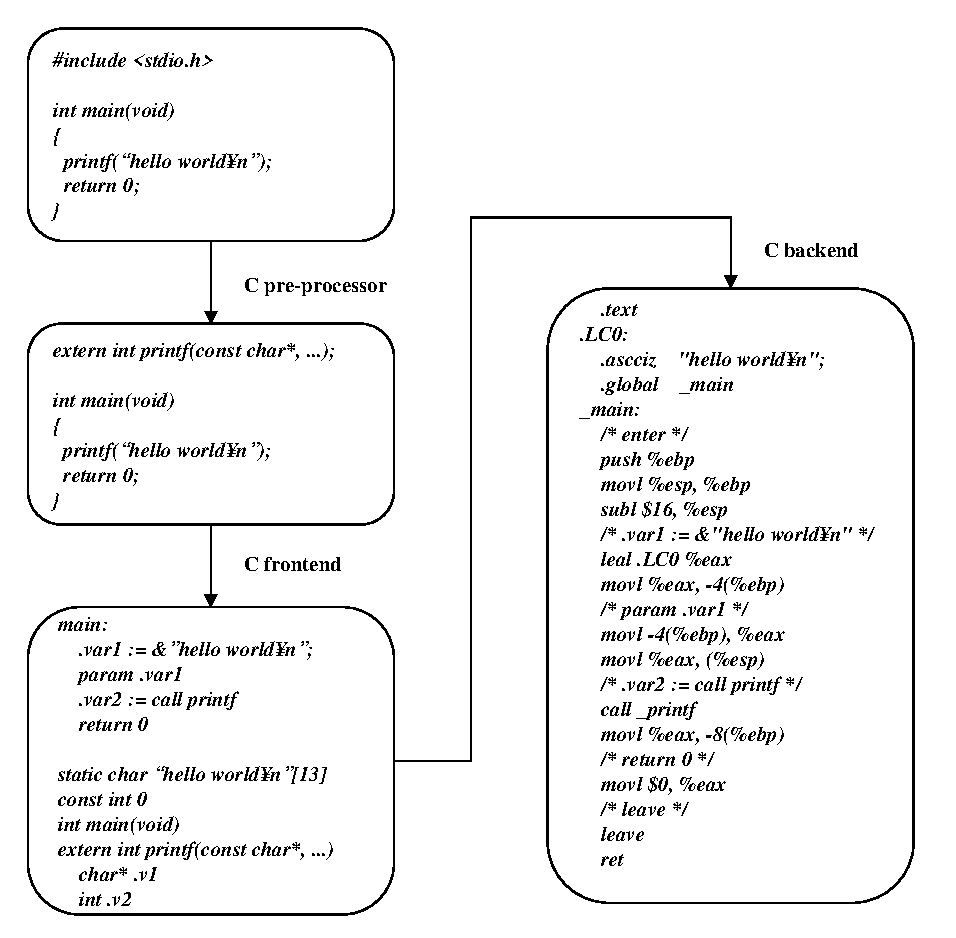
\includegraphics[width=1.0\linewidth,height=1.2\linewidth]{front_back_e.eps}
\end{latexonly}
\begin{htmlonly}
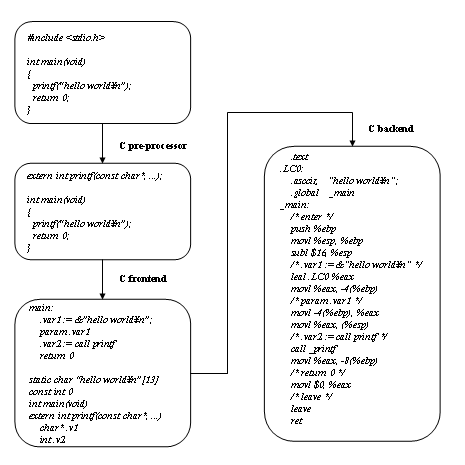
\includegraphics[width=1.2\linewidth,height=1.2\linewidth]{front_back_e.png}
\end{htmlonly}
\caption{frontend \& backend}
\label{front_back_e007}
\end{center}
\end{figure}
%% How to convert Power Point file to EPS file
%% http://keijisaito.info/arc/TeX/ve_ppfi_pdf.htm
%% ->
%% Changed. Use Metafile converter
%% Metafile to EPS Converter
%% https://wiki.lyx.org/Windows/MetafileToEPSConverter

To implement compilers for the various target processors, 
bibliography \cite{doragon} says that compilers should be devided into
 frontend \& backend.
Frontend is independent of target processsors
(depend on programming language), and backend is depend on
target processor. Figure \ref{front_back_e007} shows how they work
at programming language C `hello world'.

Frontend converts program to 3 address code and symbol table.
Backend converts outputs of frontend to target code(here, Windows/Intel code).

3 address code outputed by frontend is very simple for backend to
convert to target assembler code. Each operand of 3 address code
is an entry of symbol table, which contains name, type and storage class
or other infomation.

\begin{QandA}
Why is not Figure \ref{front_back_e007} target code optimized.

Answer : Mainly because backend which converts 3 address code to target code
doesn't optimize.

In compiler which constitute from frontend \& backend, each part
optimization makes optimized code.

This backend converts to about 3 instruction for an 3 address code.
Bibliography \cite{doragon} says that ``But if you convert 3 address code
 indiviually, you can only generate poor code'' at 9.1
(Sorry, but as you know, I just only read Japanese edition doragon book).
\end{QandA}

\begin{QandA}
\label{front_back_e003}
In figure \ref{front_back_e007} target code, address of string is saved
temporary variable. But generally, as a 3 address code,
\begin{verbatim}
param &y
\end{verbatim}
Is it allowable?

Answer : It should not be. We have to distinguish \tt{param y} and
\tt{param \&y}. And this 3 address code set including \tt{param \&y} is
redundant. On the other hand, at compile time, address of
variable, function or string literal is referenced as offset from
frame pointer or stack pointer, or label. This means target code
for \tt{param \&y} is better than obvious target code for
\begin{verbatim}
t0 := &y
...
param t0
\end{verbatim}
But it's possible to generate the same target code.
\end{QandA}

\begin{QandA}
In figure \ref{front_back_e007}, the return value of {\tt{printf}} 
is not used. It can be discarded?

Answer : It can be done at optimiezation phase.
\end{QandA}



\chapter{Lexical analisis \& syntax analisis}

\label{lex_yacc_e000}
\index{lexical analizer@lexical analizer}
\index{syntactic analysis@syntactic analysis}
As described in chpater \ref{front_back_e000}, frontend
converts program to 3 address code and symbol table.
Before this converting, frontend does lexixcal analisis
and syntax analisis. Here we described about these.

Bibliography \cite{doragon} illustrates precicely
the way of lexical analisis and syntax analisis.
Now we'll use {\tt{lex}} and {\tt{yacc}} because
they are very useful.

We can find the C language grammer in bibliography \cite{ISO}.
In bibliography \cite{KR}, \cite{SGS}, you can find 
the same kind of description.
And it is very simple to convert {\tt{yacc}} program text.
We also can find the C laugage lexicograph in bibliography \cite{ISO}.
Unfortunately, it's not simple to convert {\tt{lex}} program text, so,
it's necessary to convert it to regular expression.
\begin{htmlonly}
There are  {\tt{lex}} program text and {\tt{yacc}} program text.
in \ref{grammer_e000}.
\end{htmlonly}

\section{Syntax analisis using {\tt{yacc}} }

\label{lex_yacc_e003}
You can find that {\tt{yacc}} just report shift/reduce conflict about
{\tt{if else}}. And this conflict is recognized as `shift', and it doesn't
matter.

In the process of upper syntax analisis, we'll just make
syntax tree. For example, about {\tt{additive-expression}}

\begin{verbatim}
/* yacc program text */
%type<expr> multiplicative_expression additive_expression
...
additive_expression
  : multiplicative_expression
  | additive_expression '+' multiplicative_expression
    { $$ = new bin_expr('+',$1,$3); }
  | additive_expression '-' multiplicative_expression
    { $$ = new bin_expr('-',$1,$3); }
  ;

// Node for expression
class expr {
  ...
  // Interface for generating 3 address code
  virtual var* eval() = 0;
};

// Node for binary expression
class bin_expr : public expr {
  ...
  bin_expr(int op, expr* left, expr* right);
  var* eval();
};
\end{verbatim}

\begin{QandA}
Generally, for grammer ``A $\rightarrow$ B $|$ C D'', define
structure Sa, Sb, Sc like bellow
\begin{verbatim}
struct Sb;
struct Sc;
struct Sd;
struct Sa {
  Sb* m_Sb;
  Sc* m_Sc;
  Sd* m_Sd;
  Sa(Sb* b) : m_Sb(b), m_Sc(0), m_Sd(0) {}
  Sa(Sc* c, Sd* d) : m_Sb(0), m_Sc(c), m_Sd(d) {}
};

A : B   { $$ = new Sa($1); }
  | C D { $$ = new Sa($1,$2); }
  ;
\end{verbatim}
This way for generating syntax tree is simple and automatic.
Does it work?

Answer : It works but please take care if grammer is defined
recursively like programming lauguage C expression. For example,
a + b syntax tree contains many empty node. That is, in above
grammer, almost all are ``A $\rightarrow$ B''.
It cause use of large heap and then compiler cannot run fast.
\end{QandA}

\begin{QandA}
\label{lex_yacc_e001}
Is it OK not to generate syntax tree but to generate 3 address
code immediately in the process of upper syntax analisis.

Answer : It's OK. But in this case, you must move a 
group of 3 address codes. For example, {\tt{for}} statement
code generation is implemented like bellow if you generate
syntax tree in the process of upper syntax analisis.

\begin{verbatim}
/* yacc program */
for_statement
  : ...
  | FOR '(' expression ';' expression ';' expression ')' statement
    { $$ = new for_stmt($3,$5,$7,$9); }
  ;

// for statement code generation
void for_stmt::gen()
{
  generate 3 address code of $3
  label("begin");
  generate 3 address code of $5
  generate if result of $5 == 0 goto "end"
  generate 3 address code of $9
  generate 3 address code of $7
  generate goto "begin"
  label("end);
}
\end{verbatim}

On the other hand, if you generate 3 address code immediately in the
process of upper syntax analisis,
you must replace 3 address code of {\tt{\$7}}
and that of {\tt{\$9}}.
\end{QandA}

\section{Lexical analisis using {\tt{lex}}}
\label{lex_yacc_e004}
As described in \ref{lex_yacc_e003}, if we can use  {\tt{yacc}},
syntax analisis of C programming lauguage is not so difficult.
But please remember that lexical analizer must work well for it.
The lexical analisis point is to chose a correct token
for a lexicography which matches
regular expression
\begin{verbatim}
{nondigit}({nondigit}|{digit})*
\end{verbatim}
For this, compiler must reference symbol table at least. For example,

\begin{verbatim}
typedef int A;    /* insert `A' into symbol table. */
A a;              /* `A' isn't identifier. It's 
                     typedef-name. */

void f(void)
{
  A A = A;        /* 1st `A' is typedef-name. */
                  /* 2nd `A' isn't typedef-name. It's
                     identifier. In this case, compiler
                     doesn't look up symbol table. */
                  /* For 3rd `A', compiler looks up 
                     symbol table, and it's identifier. */
  ...
}
\end{verbatim}
When compiler detects the minimum unit of declaration,
compiler must insert it into symbol table.

\begin{verbatim}
declaration
  : declaration_specifiers init_declarator_list ';'
    { /* incorrect timing. */ }
  | ...
  ;
...
init_declarator
  : declarator     { /* Now insert symbol table. */ }
  | declarator '=' { /* Now insert symbol table. */ } initializer
  ;
...
\end{verbatim}
When compiler choses a correct token, compiler looks up symbol
table, so, the attribute of lexicography {\tt{identifier}}, {\tt{typedef-name}}
should be an entry of symbol table.
Note that compiler doesn't have to look up in {\tt{yacc}} action part.
Please reference bibliography \cite{doragon} about the attribute
of lexicography.

\begin{QandA}
Bibliography \cite{doragon} says that
the attribute of lexicography {\tt{constant}}
should be an correspond constant. But in figure
\ref{front_back_e007}, constant integer {\tt{0}}
and string literal {\tt{``hello world\verb|\|n''}}
are in symbol table. Is it necessary? What attribute 
should be for {\tt{constant}}?

Answer : {\tt{constant}} has it's type in C launguage.
And string literal storage class is {\tt{static}}.
Please reference bibliography \cite{ISO} about these.
Every constant has it's name and type, so it is natural
that compiler inserts constant into symbol table.
The attribute of lexicography {\tt{constant}} 
should be an entry of symbol table like {\tt{identifier}}
or {\tt{typedef-name}}.
\end{QandA}

\subsection{Lexical analyzer and symbol table}
\label{lex_yacc007_e}
In \ref{lex_yacc_e004}, we described that comiler must
look up symbol table for a lexicography
which matches to regular expression
\begin{verbatim}
{nondigit}({nondigit}|{digit})*
\end{verbatim}
in some cases. If you use the grammer of bibliography \cite{ISO},
{\tt identifier} and {\tt typedef-name} matches to this regular
expression. But not only variable and typedef name are in symbol table.
Tag name of structure, union and enumeration are also in symbol table.
So we'll let {\tt tag-name} be a terminal symbol and change the
grammer of bibliography \cite{ISO} like bellow.

\begin{verbatim}
struct-or-union-specifier :
  struct-or-union identifier { struct_declaration_list }
  struct-or-union { struct-declaration-list }
  struct-or-union identifier
  struct-or-union tag-name              # This rule is added.
...
enum-specifier:
  enum identifier { enumerator-list }
  enum            { enumerator-list }
  enum identifier { enumerator-list , }
  enum            { enumerator-list , }
  enum identifier
  enum tag-name                         # This rule is added.
\end{verbatim}
In the rules of {\tt struct-or-union-specifier },
1st and 2nd rule are the declaration of complete structure or union,
3rd rurle is the declaration of incomplete structure or union,
4th rule is the reference of already defined structure or union.
In the bellow example, we'll know that compiler must look up
symbol table only in necessary case.
\begin{verbatim}
typedef int T;  /* Not look up. `T' is identifier. */

T t;  /* Look up and decide `T' is typedef-name. */

struct T {  /* Not look up. `T' is identifier. */
  ...
};

void f(void)
{
  struct T t; /* Look up and decide `T' is tag-name. */
  struct T {  /* Not look up. `T' is identifier. */ 
    ...
  };
}
\end{verbatim}
Here, we'll think the case compiler should look up symbol table
or not when a lexicography matches to regular expression
{\tt \{nondigit\}(\{nondigit\}|\{digit\})*}.

\newtheorem{Method}{Method}[chapter]

\begin{Method}
\label{lex_yacc_e002}
Judge from previous token.

\begin{verbatim}
int a;          /* previous is int, so not look up.
                   `a' is identifier. */
typedef int A;  /* previous is int, so not look up.
                   `A' is identifier. */
A aa;           /* previous is ';', so look up and
                   `A' is typedef-name. */
                /* previous is typedef-name, so not look up.
                   `aa' is identifier. */
\end{verbatim}

If previous token is one of
\begin{verbatim}
void char int float double short long signed unsigned
typdef-name tag-name . -> goto
\end{verbatim}
then not look up and make it  {\tt{identifier}}.
\end{Method}

There are some problems in method \ref{lex_yacc_e002} because
compiler cannot decide to look up or not from
previous token.

\begin{verbatim}
int const a;  /* previous is const,
                 not look up?  */
typedef int A;
const A b;    /* Not good in this case. For `A',
                 compiler must look up. */
\end{verbatim}
If previous token is one of
\begin{verbatim}
volatile restrict typedef extern static register auto inline
\end{verbatim}
the same problem with {\tt{const}} occurs.

Other problem will occur when the token
should be {\tt{tag-name}}.

\begin{verbatim}
struct S {  /* previous is struct, not look up? */
  ...
};

struct S s; /* Not good. For `S', compiler must look up. */
\end{verbatim}


\begin{Method}
\label{lex_yacc_e005}
Samely as Method \ref{lex_yacc_e002}, remember previous token.
And also remember the return values of lexical analyzer
which is one of
\begin{verbatim}
void char int float double short long signed unsigned
typdef-name tag-name
const volatile restrict
typedef extern static register auto inline
\end{verbatim}
For these token, prepare global container like bellow.
\begin{verbatim}
vector<int> lexed_spec;
\end{verbatim}
This container must be cleared when one of
\begin{verbatim}
declaration
struct-declaration
parameter-declaration
\end{verbatim}
is reduced.

Bellow function tells us whether compiler should lookup
symbol table or not.
\begin{verbatim}
bool should_lookup()
{
  if ( prev == STRUCT || prev == UNION || prev == ENUM )
    return peek() != '{';

  if ( lexed_spec.empty() )
    return prev != '.' && prev != ARROW && prev != GOTO;

  return find_if(lexed_spec.begin(),lexed_spec.end(),enough)
    == lexed_spec.end();
}

bool enough(int n)
{
  If n is one of bellow, return true.
  void char int float double short long signed unsigned
  typdef-name tag-name

  If not, return false. i.e. n is one of 
  const volatile restrict
  typedef extern static register auto inline
}
\end{verbatim}
\end{Method}

There are some problems in method \ref{lex_yacc_e005}.

\begin{verbatim}
int typedef A;      /* A : Not look up because int and typedef
                       are in lexed_spec. */

A a[sizeof(const A)], b;
                    /* 1st `A' : Look up because lexed_spec is empty
                       and previous token is ';'. */
                    /* `a' : Not look up because typedef-name is
                       in lexed_spec. */
                    /* 2nd `A' : Not good. Compiler should have
                       looked up. typedef-name and const are
                       in lexed_spec. */
                    /* `b' : Not look up because typedef-name
                        and const are in lexed_spec. This is OK,
                        but type of `b' becomes const A. */

void f(A a);        /* `f' : Not look up because void is in lexed_spec. */
                    /* `A' : Not good. Compiler should have looked up.
                        void is in lexed_spec. */
                    /* `a' : Not look up because void is in lexed_spec.
                       This is OK, but type of `a' becomes void. */
\end{verbatim}

\begin{Method}
\label{lex_yacc_e006}
Samely as \ref{lex_yacc_e002}, remember previous token.
And samely as \ref{lex_yacc_e005}, remember {\tt{lexed\_spec}}.
And more, remember bellow infomation.
\begin{verbatim}
struct spec {
  type* m_type; // remember type
  int m_other;  // remember storage class or function specifier
};
stack<spec*> spec_stack;
\end{verbatim}
Before clearing {\tt{lexed\_spec}}, 
push {\tt{spec}} whihch is same with {\tt{lexed\_spec}}
to {\tt{spec\_stack}}.
And then push 0.
Bellow example shows the timing of clear, push and pop.

\begin{verbatim}
typedef short int A[3];
static int n =
/* push (static, int). clear lexed_spec. push 0. */
sizeof(A), /* `A' : Look up. pop. */
m    /* Reference spec_stack.top() */
;    /* pop. */

struct S {
  unsigned int a :
  /* push (unsigned int). clear lexed_spec. push 0. */
  sizeof(A), /* `A' : Look up. pop. */
  b[5]  /* Reference spec_stack.top() */
  ;     /* pop. */
};

int b[  /* push (int). clear lexed_spec. push 0. */
     sizeof(A)  /* `A' : Look up. */
     ]  /* pop */
     , c /* Reference spec_stack.top(). */
     ;     /* pop. */

inline void f(a,b,c)
  /* push (inline, void ()). clear lexed_spec. push 0. */
  int a;    /* `a' : Not look up because int is in lexed_spec. */
  double b; /* `b' : Not look up because double is in lexed_spec. */
  char* c;  /* `c' : Not look up because spec_stack.top() has infomation. */
  /* pop */
{
  ...
}

static void g(
/* push (static, void). clear lexed_spec. push 0. */
  FILE  /* Look up because spec_stack.top() is 0. */
  *
  fp    /* Not look up because spec_stack.top() is FILE*.  */
  /* pop */
);
\end{verbatim}

Now, we can rewrite function {\tt{should\_lookup}} like bellow.
\begin{verbatim}
bool should_lookup()
{
  if ( prev == STRUCT || prev == UNION || prev == ENUM )
    return peek() != '{';

  if ( !lexed_spec.empty() ) {
    return find_if(lexed_spec.begin(),lexed_spec.end(),enough)
      == lexed_spec.end();
  }

  if ( !spec_stack.empty() )
    return !spec_stack.top();

  return prev != '.' && prev != ARROW && prev != GOTO;
}
\end{verbatim}
\end{Method}

There is a problem about {\tt{abstract-declarator}}
in method \ref{lex_yacc_e006}.
\begin{verbatim}
typedef int T;
T f(T (T));
\end{verbatim}
where {\tt{f}} should not be same with
\begin{verbatim}
T f(T);
\end{verbatim}
But {\tt{f}} should be same with
\begin{verbatim}
T f(T (*)(T));
\end{verbatim}
In 1st declaration of {\tt{f}}, 3rd {\tt{T}} should have been
looked up and decided it {\tt{typedef-name}}.
Please note that the declaration
\begin{verbatim}
T f(T (a));
\end{verbatim}
is equivalent to
\begin{verbatim}
T f(T);
\end{verbatim}
And also, please note that
\begin{verbatim}
T (T);  // T (T) out side of parameter
\end{verbatim}
is equivalent to
\begin{verbatim}
int T;
\end{verbatim}
and
\begin{verbatim}
T f(T (T));  // T (T) at parameter scope
\end{verbatim}
is equivalent to
\begin{verbatim}
int f(int (*pf)(int));
\end{verbatim}

Above example shows that
we cannot decide whether compiler should look up or not.
But we decide like bellow.
If previous token is '(' and compiler analyzes
in parameter scope, then look up the symbol. And
if it is {\tt{typedef-name}}, its token is {\tt{typedef-name}}.
That is,

\begin{verbatim}
/* lex program */
{nondigit}({nondigit}|{digit})*   { return judge(yytext); }

// Decide token of name. identifier, typedef-name or tag-name.
int judge(string name)
{
  if ( prev == STRUCT || prev == UNION || prev == ENUM ) {
    if ( peek() == '{'; )
      return IDENTIFIER;
    if ( int r = lookup(name) )  // Only look up tag name
      return r;
    return IDENTIFIER;
  }

  if ( !lexed_spec.empty() ) {
    p = find_if(lexed_spec.begin(),lexed_spec.end(),enough);
    if ( p != lexed_spec.end() )
      return IDENTIFIER;
    if ( int r = lookup(name) )
      return r;
    return IDENTIFIER; // If not exists, not error.
  }

  if ( !spec_stack.empty() ) {
    if ( prev == '(' && analyzing parameter scope ) {
      int r = lookup(name);
      if ( r && r == TYPEDEF_NAME )
        return TYPEDEF_NAME;
      return IDENTIFIER; // If not exists, not error.
    }

    if ( spec_stack.top() )
      return IDENTIFIER;

    if ( int r = lookup(name) )
      return r;   

    return IDENTIFIER; // Maybe error, but cannot decide here.
  }

  if ( prev == '.' || prev == ARROW || prev == GOTO )
    return IDENTIFIER;

  if ( int r = lookup(name) )
    return r;

  return IDENTIFIER; // Maybe error, but cannot decide here.
}
\end{verbatim}

Compiler cannot make it error immediately even if the symbol is not in
symbol table.
\begin{verbatim}
main()  /* Not specified return type or storage class of `main'.
           lexed_spec is empty and spec_stack is empty.
           previous token is meaningless. Compiler looks up
           but not in symbol table. */
{
  printf("hello world\n");
  /* call function which is not declared.
     lexed_spec is empty and spec_stack is
     empty. previous token is '{'. Compiler looks up
     but not in symbol table. */

label:   /* Look up but not in symbol table. */
  ;

  int f(a,b,c);  /* For `a', `b', `c',
                    look up but not in symbol table. */
}
\end{verbatim}
In some cases, undeclared variable reference in expression 
must be dealt when compiler generates 3 address code.

\begin{verbatim}
int f();

int g(int a)
{
  // ...
label:      // Should be looked up `label'?
  f();

  // ...
  a ? --a : g(++a);   // ':' apears here

  struct S {
    int a : sizeof f();  // And ':' apears here too.

    // ...
  };

f:   // should be look up `f'?
  g(f());

  // ...
}
\end{verbatim}
Finaly, please consider that it sould be looked up identifier
before ':'.
The rules we discussed at this section specify that:
\begin{itemize}
\item
look up `a' at expr1 ? a : expr2 
\item
not look up `a' at int a : sizeof f();
\end{itemize}

I don't want to, if it's possible, look up label at
labeled-statement. But if it's difficult to judge,
just looking up may be simple because
we can change the way to deal with the label
at code generation routine of labeled-statement,
according to the label entried at symbol table or not.


\chapter{Symbol table}

\label{symtab_e002}

\section{Data structure of symbol table and look up}
Scope of C language constructs hierarchy as described in
bibliography \cite{ISO} 6.1.2.1 Scopes of identifiers and
6.1.2.3 Name spaces of identifiers.

We mentioned in \ref{lex_yacc_e004} that lexical analizer must look up
symbol table. For getting an entry from string, we'll use
structure like bellow.

\label{symtab_e000}
\begin{verbatim}
struct usr;  // variable in program
struct tag;  // tag in program

struct scope {
  scope* m_parent;            // outer scope
  vector<scope*> m_children;  // inner scope
  map<string,usr*> m_usrs;    // get an entry from string
  map<string,tag*> m_tags;    // get an entry from string
  static scope* current;
  static scope root;
};
\end{verbatim}
\index{scope@scope}
\index{tag@tag}
\index{usr@usr}
\index{scope@scope}

It's necessary that compiler creates a new {\tt{scope}} or sets
{\tt{scope::current}} suitably while syntax analisysing.
And it's also neccessary that compiler sets {\tt{scope::current}} suitably
while generating 3 address code.
For this, we'll change grammer described in chapter \ref{lex_yacc_e000}
like bellow.

\begin{verbatim}
compound_statement
  : '{' enter_block block_item_list leave_block '}'
  | ...
  ;

enter_block
  : {
      ...
      vector<scope*>& children = scope::current->m_children;
      scope* tmp = new scope;
      tmp->m_parent = scope::current;
      children.push_back(tmp);
      scope::current = tmp;
    }
  ;

leave_block
  : { scope::current = scope::current->m_parent; ... ; }
  ;
\end{verbatim}

It's necessary that compiler remembers the order of parameters in
parameter scope.
\begin{verbatim}
struct param_scope : scope {
  vector<usr*> m_order;   // remember the order
};

direct_declarator
  : ...
  | direct_declarator '(' enter_param_scope
                          parameter_type_list
                          leave_param_scope ')'
  | ...
  ;

enter_param_scope
  : {
      vector<scope*>& children = scope::current->m_children;
      scope* param = new param_scope;
      param->m_parent = scope::current;
      children.push_back(param);
      scope::current = param;
    }
  ;

leave_param_scope
  : { scope::current = scope::current->m_parent; ... ; }
  ;
\end{verbatim}

Now, we can write  {\tt{lookup}} of \ref{lex_yacc_e004} like bellow.
\begin{verbatim}
int lookup(string name, scope* ptr = scope::current)
{
  if ( prev == STRUCT || prev == UNION || prev == ENUM ) {
    // previous token is one of struct, union or enum
    const map<string, tag*>& tags = ptr->m_tags;
    p = tags.find(name);
    if ( p != tags.end() )
      return TAG_NAME; // found
  }
  else {
    const map<string, usr*>& usrs = ptr->m_usrs;
    p = usrs.find(name);
    if ( p != usrs.end() ) {
      // found
      if ( p->second is typedefed )
        return TYPEDEF_NAME;
      return IDENTIFIER;
    }
  }

  if ( ptr->m_parent )
    return lookup(name,ptr->m_parent); // lookup outer scope

  return 0; // not found
}
\end{verbatim}

\begin{QandA}
Variables which share the same name are defined or declared
in the same scope multiply and validly. From that, for getting
entrys from string, bellow structure is correct. Is it true?
\begin{verbatim}
struct scope {
  ...
  map<string,vector<usr*> > m_usrs;  // correspond the plural
  ...
};
\end{verbatim}

Answer : That's right. For example, it's ncessary that
we change {\tt {scope}} like above for generating correct
code for bellow program piece.
\begin{verbatim}
void f(void)
{
  void g(int);
  extern int a;
  g(a);  // reference global `a'
  int a; // hide global `a'
  g(a);  // reference local `a'
}
\end{verbatim}
`{\tt{lookup}}' decides the last entry as a attribute of token.
\end{QandA}

\begin{QandA}
I think medium variables generated by compiler are in symbol table.

Answer : You're right. But comiler doesn't have to look up symbol table
for them, so we should distingish them. Also note that medium variables
can be in restricted scope. We define new {\tt{scope}} as a derived
class like bellow.
\begin{verbatim}
struct var;  // medium variable

struct block : scope {
  vector<var*> m_vars;
};

/* yacc program text */
enter_block
  : {
      ...
      vector<scope*>& children = scope::current->m_children;
      scope* tmp = new block;  /* change to `block' */
      tmp->m_parent = scope::current;
      children.push_back(tmp);
      scope::current = tmp;
    }
  ;
\end{verbatim}
\end{QandA}

\begin{QandA}
\label{symtab_e001}
What is {\tt{tag}}? How do we can defined {\tt{tag}}?

Answer : Structre, union, enumeration and incomplete of them
are named by programmer. Here, we call it {\tt{tag}}.
The name of {\tt{tag}} and that of variable are not conflict
event thought they have the same name.

\begin{verbatim}
struct tag {
  int m_kind;  // one of struct, union and enum
  string m_name;
  const type* m_type;
  file_t m_file;
  scope* m_scope;
};
\end{verbatim}
\end{QandA}
\index{tag@tag}

\begin{QandA}
Is it necessary that {\tt{tag}} is derived from {\tt{scope}}?

Answer : It's not ncessary in C compiler, but
necessary in C++ compiler. For example,
\begin{verbatim}
struct outer {
  struct inner {
    ...
  }
  ...
};

struct inner x; /* OK in C, error in C++. */
outer::inner y; // Specify name specifier in C++
\end{verbatim}
This example shows that structure or union creates
a new {\tt{scope}} in C++ and doesn't create in C.
There is also difference in generating 3 address code.
\begin{verbatim}
struct T {
  int x;
};

struct T t;
t.x;  // In C++, member reference operator . changes scope::current
      // to `T'.
      /* In C, because type of `t' is structure, reference the offset
         and type of member `x' */
\end{verbatim}
\end{QandA}
\index{tag@tag}

\begin{QandA}
In function definition and function declaration that is not definition,
I want to distingish whether creating a new parameter scope or not.
How can I do so?

Answer : Sorry but we cannot show the elegant method.
We think that we always create a new parameter scope in
function definition and declaration, and destroy it
if it isn't necessary any more.

It may be possible by changing grammer, and the {\tt{yacc}} action part
of {\tt{enter\_param\_scope}} or {\tt{leave\_param\_scope}} 
runs if necessary.
It may be also possible by some way, and you create a new parameter
scope when reducing {\tt{enter\_param\_scope}} if and only if it is
necessary.

The way of changing grammer may not work because of complexity of
grammer, we think. For example, consider bellow.

\begin{verbatim}
function_definition
  : function_definition_begin compound_statement
  ;

function_definition_begin
  : ...
  | declaration_specifiers declarator '(' enter_param_scope
                                          type_parameter_list
                                          leave_param_scope ')'
  | ...
  ;
\end{verbatim}
Other than {\tt{yacc}} will reports conflicts,
note that function declaration can be nested.
\begin{verbatim}
int (*f(int (*a)(double b)))(double c)
/* In above grammer, the parameter scope of `f' will be the scope
   where `c' declared. */
{
  return a;  /* This will be error in spite of OK. */
}
\end{verbatim}

On the other hand, create always a new {\tt{param\_scope}}
when {\tt{enter\_param\_scope}} is reducing. The order of
creation is like bellow.
\[
{\tt{int\,\,\,(\,*f(
\underbrace{{\tt{\,int\,\,\,(*a)(
\overbrace{\tt{\,double\,\,\,b\,}}^{2})\,}}}_{1})\,)
(\underbrace{\tt{\,double\,\,\,c}\,}_{3})}}
\]
Here,  {\tt{param\_scope}} 2 and 3 should be destroyed
when leaving the scope.
\end{QandA}

\section{Variable in program and medium variable}
\label{symtab_e003}
We mentioned about {\tt{tag}} in Question \ref{symtab_e001}, but
didn't about {\tt{usr}} or {\tt{var}} which denotes
variable in program text or medium variable, respectively.
Because {\tt{var}} is based class and {\tt{usr}} is derived class,
and there are many calsses derived from {\tt{var}}.
Here, we simply show the correspond structure.

At least, {\tt{var}} must has its type infomation.
A type infomation will be referenced by frontend while generating
3 address code. For example, if frontend detects the addition of
{\tt{i}} whose type is {\tt{int}} and {\tt{d}} whose type is
{\tt{double}}, frontend generates bellow 3 address code.
\begin{verbatim}
  t0 := (double)i  # convert to double
  t1 := t0 + d     # addition of double
\end{verbatim}
And then, when backend converts to target code,
backend allocates memory or register suitably for
{\tt{i}}, {\tt{d}}, {\tt{t0}} and {\tt{t1}}.

The operands of 3 address code are {\tt{var}}. And it is
possible that variables in program text are the operand of 3 address code.
So, we define {\tt{var}} and {\tt{usr}} like bellow.
\begin{verbatim}
struct var {
  const type* m_type;  // contain its type infomation
  ...
};

struct usr : var {  // derived from var
  string m_name;    // name in program text
  flag_t m_flag;    // storage class or other infomation
  file_t m_file;    // file position
  ...
};
\end{verbatim}
Please reference later chapter about {\tt{var}} more
precicely.



\chapter{3 address code}

\label{_3ac_e001}
Chapter 8 of bibliography \cite{doragon} says that
which kinds of 3 address code are necessary.
Here, we'll think about the set of 3 address code for C compiler.
3 address code can be coded like below structure.
\index{3 address code@3 address code}
\begin{verbatim}
struct var;  // variable. entry of symbol table.

struct tac {
  var* x;
  var* y;
  var* z;
  tac(var* xx, var* yy, var* z) : x(xx), y(yy), z(zz) {}
};
\end{verbatim}
For examle, 3 address code of addition is
derived from {\tt{tac}} like below.
\begin{verbatim}
struct add3ac : tac {
  add3ac(var* x, var* y, var* z) : tac(x,y,z) {}
};
\end{verbatim}
Chapter 8 of bibliography \cite{doragon} says that
it's necessary to distinguish floating-point addition and
integer addition. In our case, it's possible to distinguish
them from {\tt {m\_type}} member of operand. i.e.
\begin{verbatim}
void f(add3ac* p)
{
  const type* T = p->x->m_type;
  if ( T->real() )
    ...  // floating-point addtion
  else
    ...  // integer addtion
}
\end{verbatim}
So, we'll generate {\tt{add3ac}} for both floating-point addition
and integer addition. Frontend must generate 3 address code
of which operands make sense.

When {\tt{function-definition}} is reduced, frontend generates
3 address codes. For example, for a piece of program code
\begin{verbatim}
extern int printf(const char*, ...);

int f(void)
{
   int a = 1;
   a = (a + 2) * 3;
   return printf("a = %d\n",a);
}
\end{verbatim}
frontend generates 3 address codes like below.
\begin{verbatim}
f:
        a := 1
        t0 := a + 2
        t1 := t0 * 3
        a := t1
        t2 := &"a = %d\n"
        param t2
        param a
        t3 := call printf
        return t3
\end{verbatim}

\begin{QandA}
How do we use members of {\tt{tac}}?

Answer : In optimization phase of 3 address codes, we want to
investigate usage or definition of operands. See chapter 10 in
bibliography \cite{doragon} about ud-chain and du-chain.
{\tt{x}} denotes the definition and {\tt{y, z}} denote the usage.
\end{QandA}

\begin{QandA}
I want add virtual function into {\tt{tac}} for generating target
code. Is it OK?

Answer : Sorry, but it isn't OK because frontend doesn't have to
generate target code and frontend and backend must be build in
implementation. I think you want to do like below.
\begin{verbatim}
struct tac {
  ...
  virtual void gen_target() const = 0;
};

void backend::tac2target(const vector<tac*>& code)
{
  // convert a 3 address code to some target codes automatically.
  for_each(code.begin(),code.end(),mem_fun(&tac::gen_target));
}
\end{verbatim}
Instead of above, you can code like below.
\begin{verbatim}
struct backend::table : map<string, void (*)(const tac*)> {
  table()
  {
    (*this)[typeid(assign3ac).name()] = assign;
    (*this)[typeid(add3ac).name()] = add;
    (*this)[typeid(sub3ac).name()] = sub;
    (*this)[typeid(mul3ac).name()] = mul;
    ...
  }
};

void backend::tac2target(const vector<tac*>& code)
{
  for_each(code.begin(),code.end(),gencode);
}

void backend::gencode(const tac* p)
{
  table[typeid(*p).name()](p);
}

void backend::assign(const tac* p)
{
  // Do the same work with assign::gen_target, please.
}
\end{verbatim}
\end{QandA}

\section{{\tt{x := y}}}

A class coresspond to {\tt{x := y}} can be defined like below.
\begin{verbatim}
struct assign3ac : tac {
  assign3ac(var* x, var* y) : tac(x,y,0) {}
};
\end{verbatim}
The type of operand is one of scalar, structure or union. But not
array because assignment of array is not defined in C language.
Backend can distingish various assignments from the type of {\tt{x}}.
Frontend must generates {\tt{x := y}} of which operands make sense.

\section{{\tt{x := y * z}}}

Multiplications in C language are defined for arithmetic type operands.
So the type of {\tt{y}} or {\tt{z}} must be arithmetic.
Backend can distingish various multiplications from the type of {\tt{x}}.
Frontend must generates {\tt{x := y * z}} of which operands make sense.

\section{{\tt{x := y / z}}}

For divisions, samely as multiplications,
backend can distingish various divisions from the type of {\tt{x}}.
Frontend must generates {\tt{x := y / z}} of which operands make sense.

\begin{QandA}
For {\tt{x := y}}, is the type of {\tt{x}} {\it compatible}
\index{compatible@compatible}
with that of {\tt{y}}?  Samely, for 
{\tt{x := y * z}} and {\tt{x := y / z}},
the types of {\tt{x}}, {\tt{y}} and {\tt{z}} are
{\it compatible} with each other?

Answer : It's not, because the none-{\it compatible} condition
is effective considering optimization. For example,
\begin{verbatim}
long int f(unsigned int a, int b){ return a * b; }
\end{verbatim}
For above function, fronend may generate 3 address codes
like below.
\begin{verbatim}
f:
    t0 := (unsigned int)b    # t0 : unsigned int
    t1 := a * t0             # t1 : unsigned int
    t2 := (long int)t1       # t2 : long int
    return t2
\end{verbatim}
According to the specification of C language,
arithmetic conversion and {\tt{return}} statement conversion
will be ocurred, and above 3 address codes are correct.
But frontend can know that converion from {\tt{int}} to {\tt{unsigned int}}
is equivalent to assignment, and the existence of sign
does not affect the resut of integer multiplication.
And frontend can eliminate first conversion code.
And more, if backend assigns the same space
to {\tt {int}} and {\tt {long int}}, and if frontend can know
that, third converions code can be eliminated.
In this case, optimized 3 address codes are like below.
\begin{verbatim}
f:
    t1 := a * b             # t1 : unsigned int
    return t1
\end{verbatim}
But please take care if {\tt{f}} returns the result of division
instead of multiplication. In this case, frontend cannot convert
samely. Generally, not only operand size, but
also the existence of sign affects the result of integer
division. If backend assigns the same space
to {\tt {int}} and {\tt {long int}}, and if frontend can know
that, frontend can eliminate arithmetic conversion
for division {\tt {int}} and {\tt {long int}}.
\end{QandA}

\section{{\tt{x := y \% z}}}

Moduli are defined for integer operand.
Backend can distingish various moduli from the type of {\tt{x}}.
Frontend must generates {\tt{x := y \% z}} of which operands make sense.

\section{{\tt{x := y + z}}}

Additions are defined for arithmetic type operands.
And also defined for pointer to object type
and integer, and integer and pointer to object type.
In this case, the result of addition is the pointer type.
Frontend must generates {\tt{x := y + z}} of which operands make sense.

\section{{\tt{x := y - z}}}

Subtraction are defined for arithmetic type operands.
And also defined for pointer to object type
and integer. But not defined for integer and pointer to object type.
And more, defined for pointer to object type and pointer that is
compatible with it. The result type is {\tt{long int}}.

\section{{\tt{x := y << z}}, {\tt{x := y >> z}}}

Left shift first operand is integer type. Second operand is {\tt{int}}.
Normal arithmetic conversion is not applied to left shift.
The result type is the same type of first operand.

Right shift operands are restricted samely with left shift.
Normally, if first operand type has sign, right shift 
is implemented as arithmetic shift. otherwise right shift
is equal to logical shift. But it depends on implementation.

\section{{\tt{x := y \& z}}, {\tt{x := y \^{} z}}, {\tt{x := y | z}}}

Bitwise and, exclusive-or, or are defined for integer operands.

\section{{\tt{x := -y}}, {\tt{x := \~{}y}}}

Unary minus is defined for arithmetic operand.
Bitwise-not is defined for integer operand.

\section{{\tt{x := (type)y}}}

The class according to 3 address code for type conversion is like
below.
\begin{verbatim}
struct cast3ac : tac {
  const type* m_type;   // contain type
  cast3ac(var* x, var* y, const type* t) : tac(x,y,0), m_type(t) {}
};  
\end{verbatim}

\section{{\tt{x := \&y}}}

The type of {\tt{x}} is pointer to the type of {\tt{y}}.

\begin{QandA}
Unary {\tt{\&}} operator is defined for {\it lvalue}.
Does {\tt {y}} have {\it lvalue} in {\tt{x := \&y}}?

Answer : No. First, note that 3 address code is not
equal to programming language C. For other programming
languages, the same 3 addres code set described here
can be used for implementing compiler. Frontend generates
3 address code of which operands make sense, in every case.
For medium variable {\tt{y}} which doesn't have {\it lvaue},
compiler may generate {\tt{x := \&y}}.
\end{QandA}

\section{{\tt{x := *y}}}

The type of {\tt{y}} must be pointer to object type,
and the type of {\tt{x}} is the object type.
Backend can distingish various {\tt{x := *y}} from the type of {\tt{x}}.

\section{{\tt{*y := z}}}

For both operand {\tt{y}} and {\tt{z}}, we regard source operands.
The structure according this 3 address code is like below.
\begin{verbatim}
struct invladdr3ac : public tac {
  invladdr3ac(var* y, var* z) : tac(0,y,z) {}
};
\end{verbatim}
The type of {\tt{y}} must be pointer to object type,
and the type of {\tt{z}} is the object type.
Backend can distingish various {\tt{*y := z}} from the type of {\tt{z}}.

\section{\tt{x[y] := z}, \tt{x := y[z]}}
\label{3ac_e004}
For {\tt{x[y] := z}}, the type of {\tt{x}} is aggregate, i.e.
one of structure, union and array.
Samely, for {\tt{x := y[z]}}, the type of {\tt{y}} is aggregate.
These 3 addres codes may be
generated for member reference or subscripting operator for array.
Backend can distingish various {\tt{x[y] := z}} from the type of
{\tt{z}}, and {\tt{x := y[z]}} from the type of {\tt{x}}.

\section{{\tt{x := call y}}, {\tt{call y}}, {\tt{param y}}}

\label{_3ac_e000} These are 3 address code for function call.
The structure according to these are like below.
\begin{verbatim}
struct param3ac : tac {
  param3ac(var* y) : tac(0,y,0) {}
};

struct call3ac : tac {
  call3ac(var* x, var* y) : tac(x,y,0) {}
};
\end{verbatim}
Frontend must generate {\tt{param}} or {\tt{param}}s continually
which is or are referenced by {\tt{call}}, just before generating
{\tt{call}}.

For {\tt{x := call y}}, the type of {\tt{x}} is one
of scalar, structure or union.
The type of {\tt{y}} is function or pointer to function.
If member {\tt{x}} is zero-pointer, it denotes that
function return value is not used.

For {\tt {param y}}, the type of {\tt{y}} is one of
scalar, structure or union.

Backend can distingish various 
{\tt{x := call y}}, {\tt{call y}} or {\tt{param y}}
from the type of operands.

\section{{\tt{return}}, {\tt{return y}}}

The type of {\tt{y}} is one of scalar, structure or union.

\section{{\tt{goto label}}, {\tt{if y op z then goto label}}, {\tt{label:}}}
\label{_3ac_e002}
These represents unconditional jump, conditional jump and
jump address,  respectively. The structure according to these are
like below.
\begin{verbatim}
struct goto3ac : tac {
  to3ac* m_to;  // contain jump address
  enum op { NONE, EQ, NE, LE, GE, LT, GT };
  op m_op;
  goto3ac() : tac(0,0,0), m_to(0), m_op(NONE) {}
  goto3ac(op op, var* y, var* z) : tac(0,y,z), m_to(0), m_op(op) {}
};

struct to3ac : tac {
  vector<goto3ac*> m_goto;  // contain referencing jumps
  to3ac() : tac(0,0,0) {}
};
\end{verbatim}
Unconditional jump are treated as special case of conditional jump.
Conditional jump operators (above {\tt{enum op}} member) 
are the same meaning with 
{\tt{==}}, {\tt{!=}}, {\tt{<=}}, {\tt{>=}}, {\tt{<}}, {\tt{>}}
in C language.
Frontend must generates these 3 address codes of which operands make sense.
Backend can distingish various {\tt{if y $op$ z then goto label}}
from the type of {\tt{y}}.

\begin{QandA}
Why is jump address implemented as 3 address code?

Answer : In optimization phase, we'll want to invesigate
the infomation described in above structure. So, for example,
{\tt{string}} is not enough to express jump address.
\end{QandA}

\section{ {\tt{x := va\_start y}}, {\tt{x := va\_arg y, type}}, {\tt{va\_end3ac}}}

In some implementations of backend,
these are implemented as C preprocessor macro.
But in other implementations, it's difficult to implement just using
C preprocessor macro. If backend can generate target code
for these 3 address code, it is simple.

\section{alloca x, y}
\label{_3ac_e003}
Variable length array in specification ISO C. 
\begin{verbatim}
void f(int n)
{
  int a[n];  /* variable length arrray */
  ...
}
\end{verbatim}
3 address code for this program is like below
\begin{verbatim}
f:
    t0 := 4 * n    # assume sizeof(int) = 4
    alloca a, t0   # assign t0 bytes memory for `a'
    ...
\end{verbatim}

\section{asm ``string''}

{\tt{asm-declaration}} is in ISO C++ but not in C.
Not necessary but we can change grammer.




\chapter{Type}

\label{type_e001}
We mentioned in chapter \ref{symtab_e002} that
frontend inserts a variable in program text into symbol table
for the declaration. One of attributes of a variable is it's type.
And we also mentioned in chapter \ref{_3ac_e001} that
frontend must generates every 3 address code of which operands make
sense, especially its type.

In this chapter, we'll think about the way to express types.
Bibliography \cite{doragon} chapter 6 suggests that we
use {\em type expression} for this purpose. For example,
\begin{verbatim}
void (*signal(int, void (*)(int)))(int);
\end{verbatim}
{\em Type expression} for this declaration becomes figure
\ref{type_e006}.

\hspace{0.5cm}
\begin{figure}[htbp]
\begin{center}
%%\begin{latexonly}
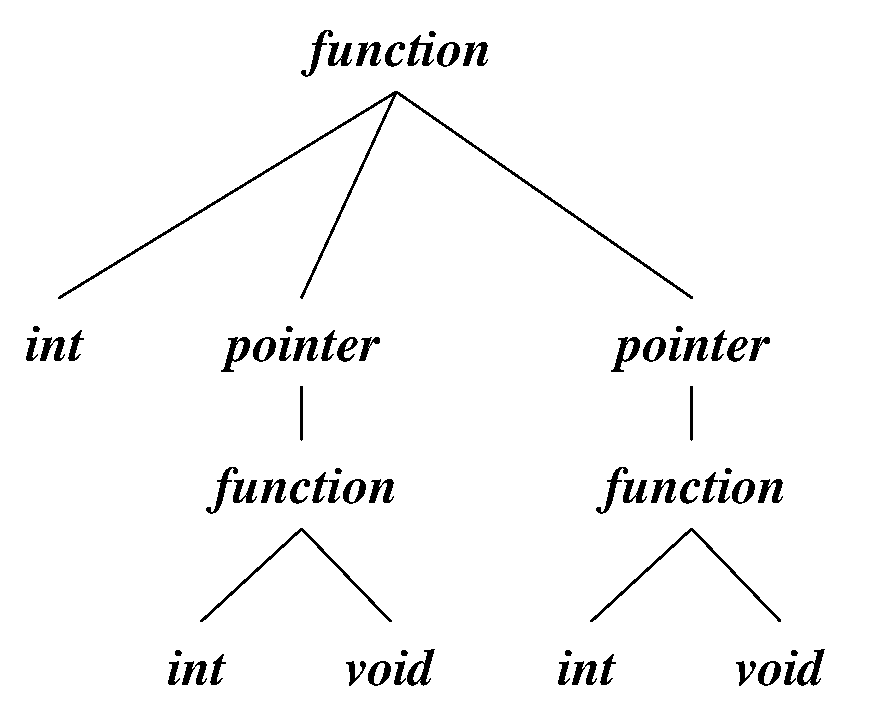
\includegraphics[width=0.5\linewidth,height=0.5\linewidth]{type_expr.eps}
%%\end{latexonly}
%%\begin{htmlonly}
%%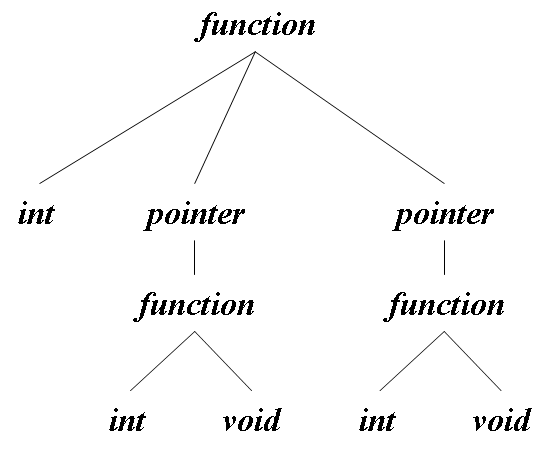
\includegraphics{type_expr.png}
%%\end{htmlonly}
\caption{{\em Type expression} of {\tt{signal}}}
\label{type_e006}
\end{center}
\end{figure}

That is, type can be expressed by tree.

Bibliography \cite{doragon} chapter 6 says that
{\em type expression} should be expressed by {\em dag}
(direct acyclic graph) not normal tree, because
compiler can judge equivalency of type easily. Frontend of C compiler
must also judge whether type $T_1$ is {\it compatible} with
type $T_2$, so we'll use {\em dag}. Figure \ref{type_e000}
shows {\em dag} for {\tt{signal}}.

\hspace{0.5cm}
\begin{figure}[htbp]
\begin{center}
%%\begin{latexonly}
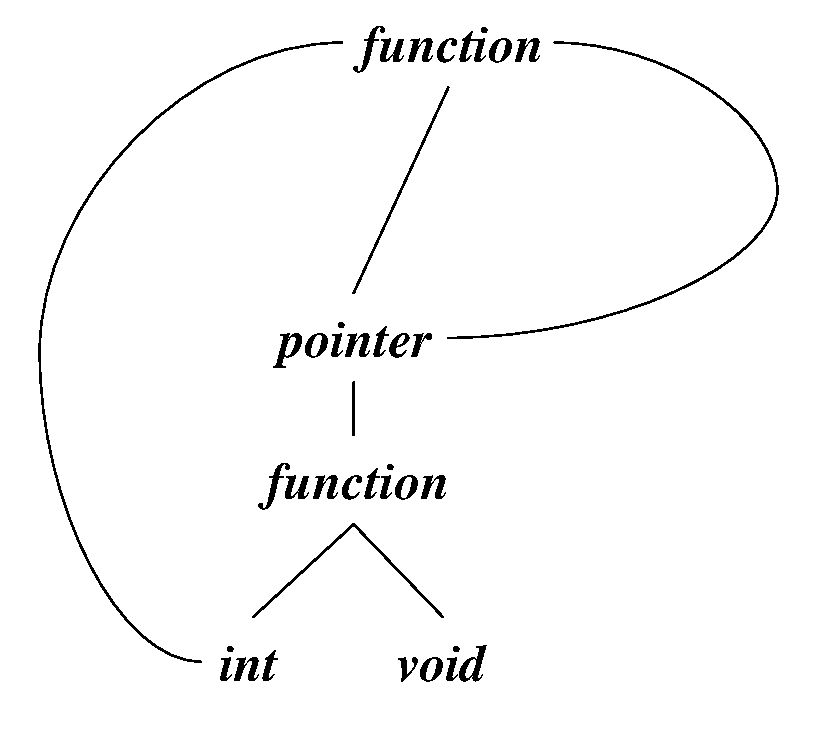
\includegraphics[width=0.5\linewidth,height=0.5\linewidth]{dag.eps}
%%\end{latexonly}
%%\begin{htmlonly}
%%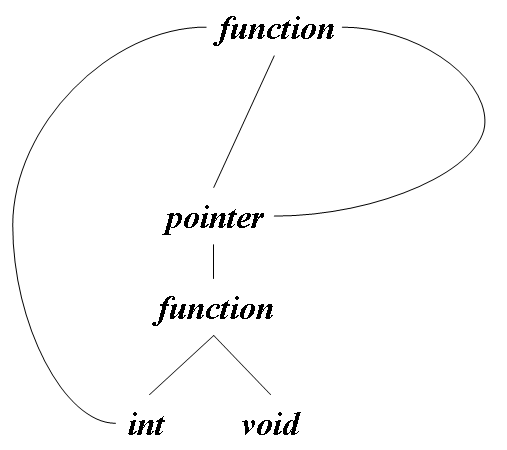
\includegraphics[width=0.3\linewidth,height=0.3\linewidth]{dag.png}
%%\end{htmlonly} 
\caption{{\em dag} of {\tt{signal}}}
\label{type_e000}
\end{center}
\end{figure}

Now, we'll define base class to judge {\it compatibility}.
\begin{verbatim}
class type {
public:
  ...
  virtual bool compatible(const type* that) const
  {
    return this == that->unqualified();
  }
  ...
};
\end{verbatim}
Please note that the equality of type can be judged by
comparing the address of types.
Other many virtual function for {\tt{type}} are necessary,
but in this chapter, we just think about {\it compatiblity} of type.

\section{Basic type}

Below table shows C language basic type and its class.

%%\begin{latexonly}
\vspace{0.5cm}
%%\end{latexonly}

\begin{tabular}{|l|l|} \hline
C language & its class \\ \hline
{\tt{void}} & {\tt{void\_type}} \\ \hline
{\tt{char}} & {\tt{char\_type}} \\  \hline
{\tt{signed char}} & {\tt{schar\_type}} \\  \hline
{\tt{unsigned char}} & {\tt{uchar\_type}} \\  \hline
{\tt{short int}} & {\tt{short\_type}} \\  \hline
{\tt{unsigned short int}} & {\tt{ushort\_type}} \\  \hline
{\tt{int}} & {\tt{int\_type}} \\ \hline
{\tt{unsigned int}} & {\tt{uint\_type}} \\  \hline
{\tt{long int}} & {\tt{long\_type}} \\ \hline
{\tt{unsigned long int}} & {\tt{ulong\_type}} \\ \hline
{\tt{long long int}} & {\tt{long\_long\_type}} \\ \hline
{\tt{unsigned long long int}} & {\tt{ulong\_long\_type}} \\ \hline
{\tt{float}} & {\tt{float\_type}} \\ \hline
{\tt{double}} & {\tt{double\_type}} \\ \hline
{\tt{long double}} & {\tt{long\_double\_type}} \\ \hline
\end{tabular}

%%\begin{latexonly}
\vspace{0.5cm}
%%\end{latexonly}

For example, {\tt{int\_type}} is defined like below.
\begin{verbatim}
class int_type : public type {
  static int_type obj;  // Only object
  int_type(){}          // private constructor
public:
  static const int_type* create(){ return &obj; }
};
\end{verbatim}

\section{Pointer}
\label{type_e003}
Pointer can be defined like below.
\begin{verbatim}
class pointer_type : public type {
  const type* m_T;  // referenced type
  pointer_type(const type* T) : m_T(T) {}
  typedef map<const type*, const pointer_type*> table_t;
  static table_t table;
public:
  static const pointer_type* create(const type* T)
  {
    table_t::const_iterator p = table.find(T);
    if (p != table.end())
      return p->second;  // already exists, return it.
    else
      return table[T] = new pointer_type(T);
  }
  bool compatible(const type* T) const
  {
    typedef const pointer_type PT;
    PT* that = dyanmic_cast<PT*>(T);
    if (!that)
      return false;
    return this->m_T->compatible(that->m_T);
  }
  ...
};
\end{verbatim}

\section{Qualifier}
\label{type_e002}
There are 3 qualifiers {\tt{const}}, {\tt{volatile}} and {\tt{restrict}}
in C language.
For example, {\tt{const}} can be expressed like below.
\begin{verbatim}
class const_type : public type {
  const type* m_T;  // qualified type
  const_type(const type* T) : m_T(T) {}
  static map<const type*, const const_type*> table;
public:
  // Return type is not const const_type*. It's const type*.
  static const type* create(const type* T);

  // Same with pointer_type::compatible
  bool compatible(const type* T) const;
  ...
};
\end{verbatim}
Someone may want to implement \tt{const\_type::create}
like {\tt{pointer\_type::create}}. But see below example:
\begin{verbatim}
typedef const int CI;     // const_type(int_type)
typedef volatile int VI;  // volatile_type(int_type)
volatile CI vci;  // volatile_type(const_type(int_type))
const VI cvi; // Not const_type(volatile_type(int_type))
              // Make it volatile_type(const_type(int_type))
const CI cci;  // Not cosnst_type(const_type(int_type))
               // Make it same with type of CI
\end{verbatim}
This example illustrates it's necessary to make more effort
to implement \tt{const\_type::create}. Other implementation
may chose a class which expresses all qualifier. It's necessary
to use same type object to express same type. If not,
{\it dag} implementation should be reviewed.

\section{Array}

Array has its element type and dimension, so can be defined like below.

\begin{verbatim}
class array_type : public type {
  const type* m_T;  // element type
  int m_dim;        // dimension
  array_type(const type* T, int dim) : m_T(T), m_dim(dim) {}
  ...
public:
  bool compatible(const type* T) const
  {
    typedef const array_type AT;
    AT* that = dynamic_cast<AT*>(T);
    if (!that)
      return false;
    if (!this->m_T->compatible(that->m_T))
      return false;
    if ( this->m_dim && that->m_dim )
      return this->m_dim == that->m_dim;
    return true;  // one is, or both are incomplete array.
  }
  ...
};
\end{verbatim}
See below declarations:
\begin{verbatim}
int a[10];
...
extern int a[];
\end{verbatim}
In 1st declaration, type of \tt{a} is
\tt{array\_type(int\_type, 10)} and 2nd declaration,
\tt{array\_type(int\_type, 0)}. 2 types are not
same, but are compatible, so 2nd declaration is
not error. Frontend may register the type of \tt{a}
as \tt{array\_type(int\_type, 10)} not
\tt{array\_type(int\_type, 0)}.

To digress a little, array cannot or should not be qualified.
For the declarations
\begin{verbatim}
typedef int A[10][20];
const A a;
\end{verbatim}
frontend should constitute {\em type expression} of {\t{a}}
like figure \ref{type007}. Figure \ref{type008} is not fine.
\begin{figure}[htbp]
\begin{center}
%%\begin{latexonly}
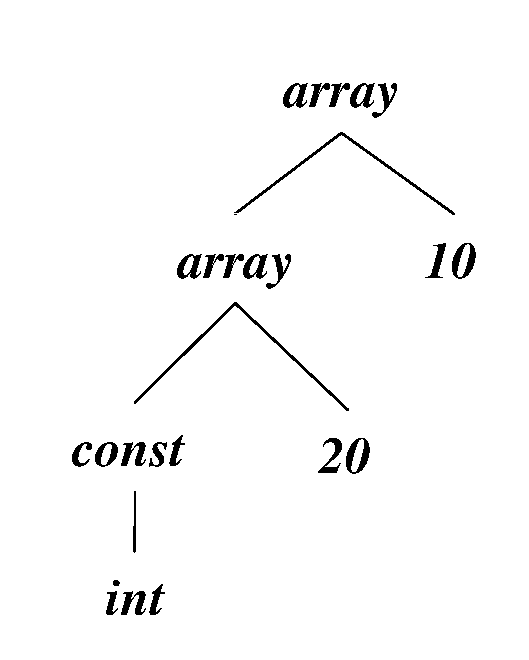
\includegraphics[width=0.4\linewidth,height=0.5\linewidth]{correct_array.eps}
%%\end{latexonly}
%%\begin{htmlonly}
%%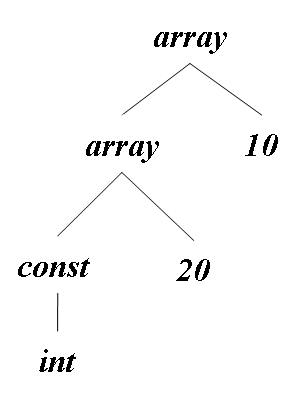
\includegraphics{correct_array.png}
%%\end{htmlonly}
\caption{correct {\em type expression} of {\tt{a}}}
\label{type007}
\end{center}
\end{figure}
\begin{figure}[htbp]
\begin{center}
%%\begin{latexonly}
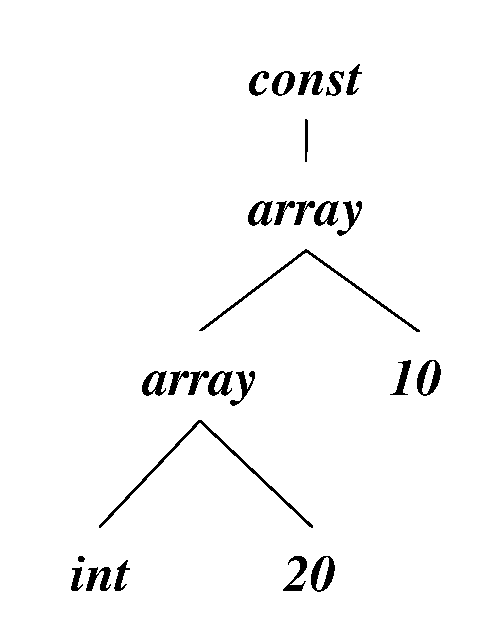
\includegraphics[width=0.4\linewidth,height=0.5\linewidth]{incorrect_array.eps}
%%\end{latexonly}
%%\begin{htmlonly}
%%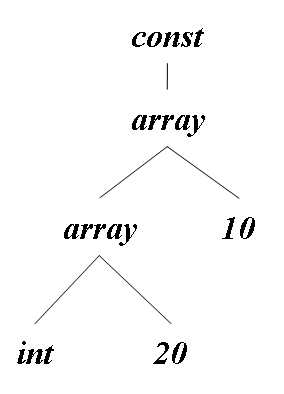
\includegraphics{incorrect_array.png}
%%\end{htmlonly}
\caption{incorrect {\em type expression} of {\tt{a}}}
\label{type008}
\end{center}
\end{figure}

\section{Function}

Function can be defined like below.
\begin{verbatim}
class func_type : public type {
  const type* m_T;              // return type
  vector<const type*> m_param;  // parameter types
  ...
public:
  bool compatible(const type*) const;
}
\end{verbatim}

Override member function {\tt{func\_type::compatible}}
becomes a little complicated.

\begin{verbatim}
bool func_type::compatible(const type* T) const
{
  typedef const func_type FT;
  FT* that = dynamic_cast<FT*>(T);
  if (!that)
    return false;  // not function
  if (!this->m_T->compatible(that->m_T))
    return false;  // not compatible return type
  if (this->m_param.size() != that->m_param.size()) {
    // possible old style, but here simply return false
    return false;
  }
  vector<const type*>& u = this->m_param;
  vector<const type*>& v = that->m_param;
  pair<IT,IT> p = mismatch(u.begin(),u.end(),v.begin(),::compatible);
  return p == make_pair(u.end(),v.end());
}
\end{verbatim}

\subsection{Variable arguments}
\label{type_e004}
In C language, function can take variable arguments.
We denotes class {\tt{ellipsis\_type}} to be ellipsis ( \tt{...}).
For example, the declaration in {\tt{stdio.h}},
\begin{verbatim}
extern int printf(const char* fmt, ...);
\end{verbatim}
for this declaration, frontend constructs {\em type expression}
like figure \ref{type_e009}.
\begin{figure}[htbp]
\begin{center}
%%\begin{latexonly}
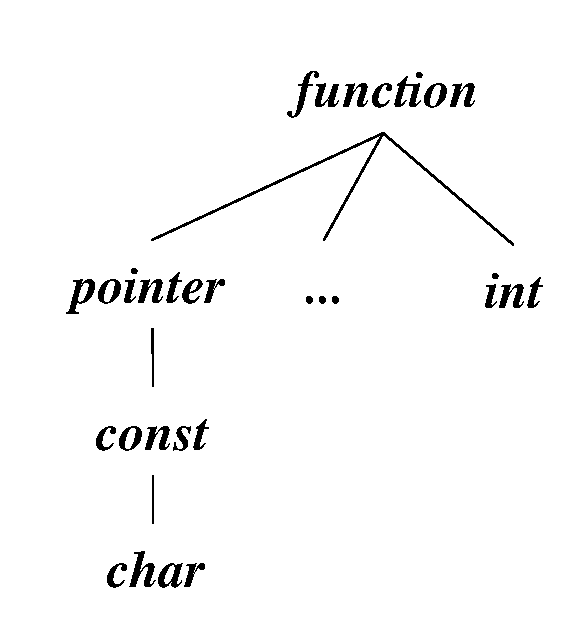
\includegraphics[width=0.5\linewidth,height=0.5\linewidth]{ellipsis_type.eps}
%%\end{latexonly}
%%\begin{htmlonly}
%%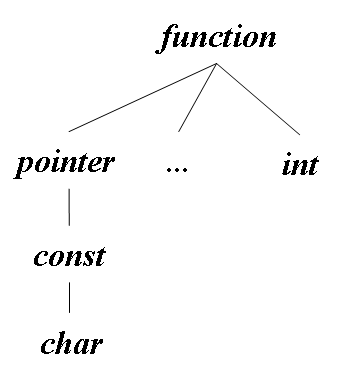
\includegraphics{ellipsis_type.png}
%%\end{htmlonly}
\caption{{\em type expression} of {\tt{printf}}}
\label{type_e009}
\end{center}
\end{figure}

\section{Tagged types}
\label{type_e010}
In C language, sturcture, union or enumeration is
associated with its tag. And its tag is associated
with its type, too. Here, we'll think about such types.
For example,
\begin{verbatim}
struct S { int m; } a;
void f(void)
{
  struct S { int m; } b;
  a = b; /* error */
}
\end{verbatim}
Compiler outputs error message like the assignment is applied for 
not compatible structure objects. This example shows
that structure is associated with its tag, not object layout.

\subsection{Structure, union}

Structure or union are referenced its member offset and type by name.
Not only tag and members, but also layout infomation should be
contained.

\begin{verbatim}
class record_type : public type {
  tag* m_tag;  // tag
  vector<usr*> m_member;  // member

  // layout infomation of structure or union
  map<string, pair<int, const type*> > m_layout;
  ...
public:
  bool compatible(const type* that) const
  {
    typedef const record_type RT;
    RT* that = dynamic_cast<RT*>(T);
    if (this == that)
      return true;
    typedef const const incomplete_tagged_type ITT;
    ITT* itt = dynamic_cast<ITT*>(T);
    if (!itt)
      return false;
    return m_tag == itt->get_tag();
  }
  ...
};
\end{verbatim}

\subsection{Enumeration}

Frontend must add enumeration members into symbol table, not into
its type. This is different with structure or union. 
\begin{verbatim}
class enum_type : public type {
  tag* m_tag;
  ...
public:
  // judge samely with record_type::compatible
  bool compatible(const type* T) const;
  ...
};
\end{verbatim}

\subsection{Incomplete tagged type}

It's possible to declare structure, union and enumeration without
members in C language. But please note that incomplete tagged type
is necessary for parsing or analising
complete structure, union and enumeration type.
For example,
\begin{verbatim}
struct tree {  /* add tag for struct tree into symbol table */

  struct tree* left;  /* lookup symbol table and know struct tree
                         is incomplete structure type */
  struct tree* right;
  int v;
}; /* struct tree becomes complete structure type */

enum E { /* add tag for enum E into symbol table */

   a = sizeof(enum E), /* lookup symbol table and know enum E
                          is incomplete type. This is error */
   b,
};
\end{verbatim}

Incomplete tagged type is defined like below.
\begin{verbatim}
class incomplete_tagged_type : public type {
  tag* m_tag;
  ...
public:
  // judge samely with record_type::compatible
  bool compatible(const type* T) const;
  ...
};
\end{verbatim}

\section{Bit field}

We don't have to search if bit field is compatible
to type $T$, because bit field is member of structure
or union. Structure or union {\it compatiblity} is
depend its tag. But it's necessary to remember
the member is bit field.

\begin{verbatim}
class bit_field_type : public type {
  int m_bit;          // number of bit
  const type* m_T;    // integer type
  ...
};
\end{verbatim}


\chapter{Declaration}

\section{Calcuration {\em type expression}}
We described how to express type in chapter \ref{type_e001}.
In this chapter, we'll think about how to calcurate
{\em type expression} from declaration of C language.

First, we'll start to think about below declaration, specifically.
\begin{verbatim}
int f(double (*)(void));
\end{verbatim}
Figure \ref{decl_e001} shows syntax tree of this declaration.
\begin{figure}[htbp]
\begin{center}
\begin{htmlonly}
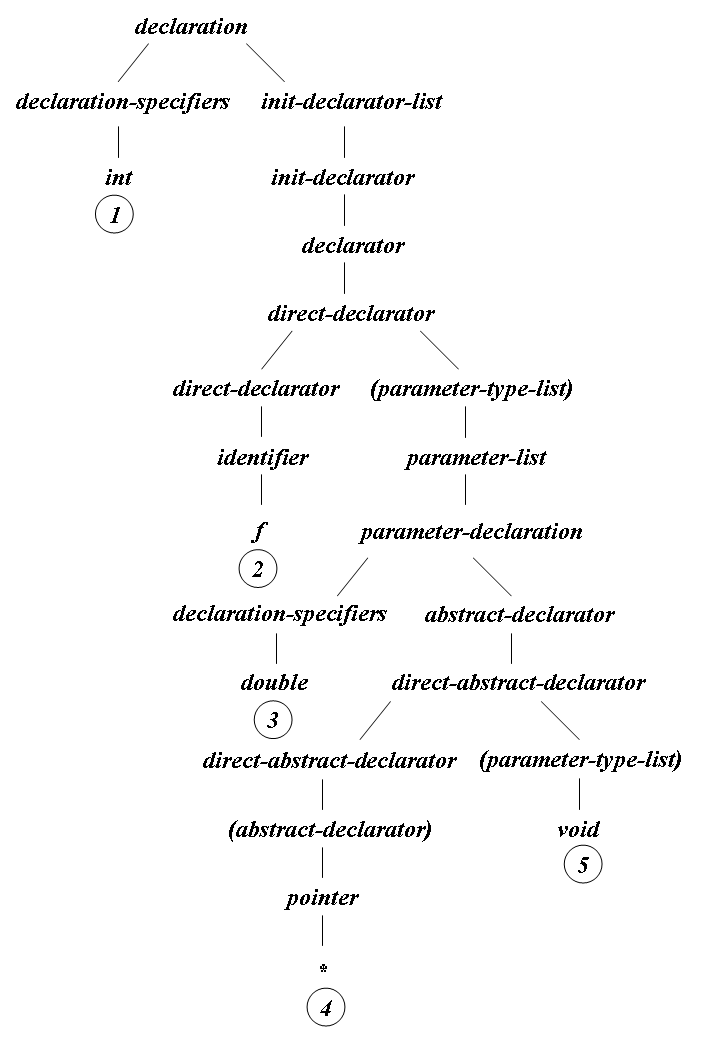
\includegraphics[width=1.0125\linewidth,height=1.4175\linewidth]{decl001.png}
\end{htmlonly}
\begin{latexonly}
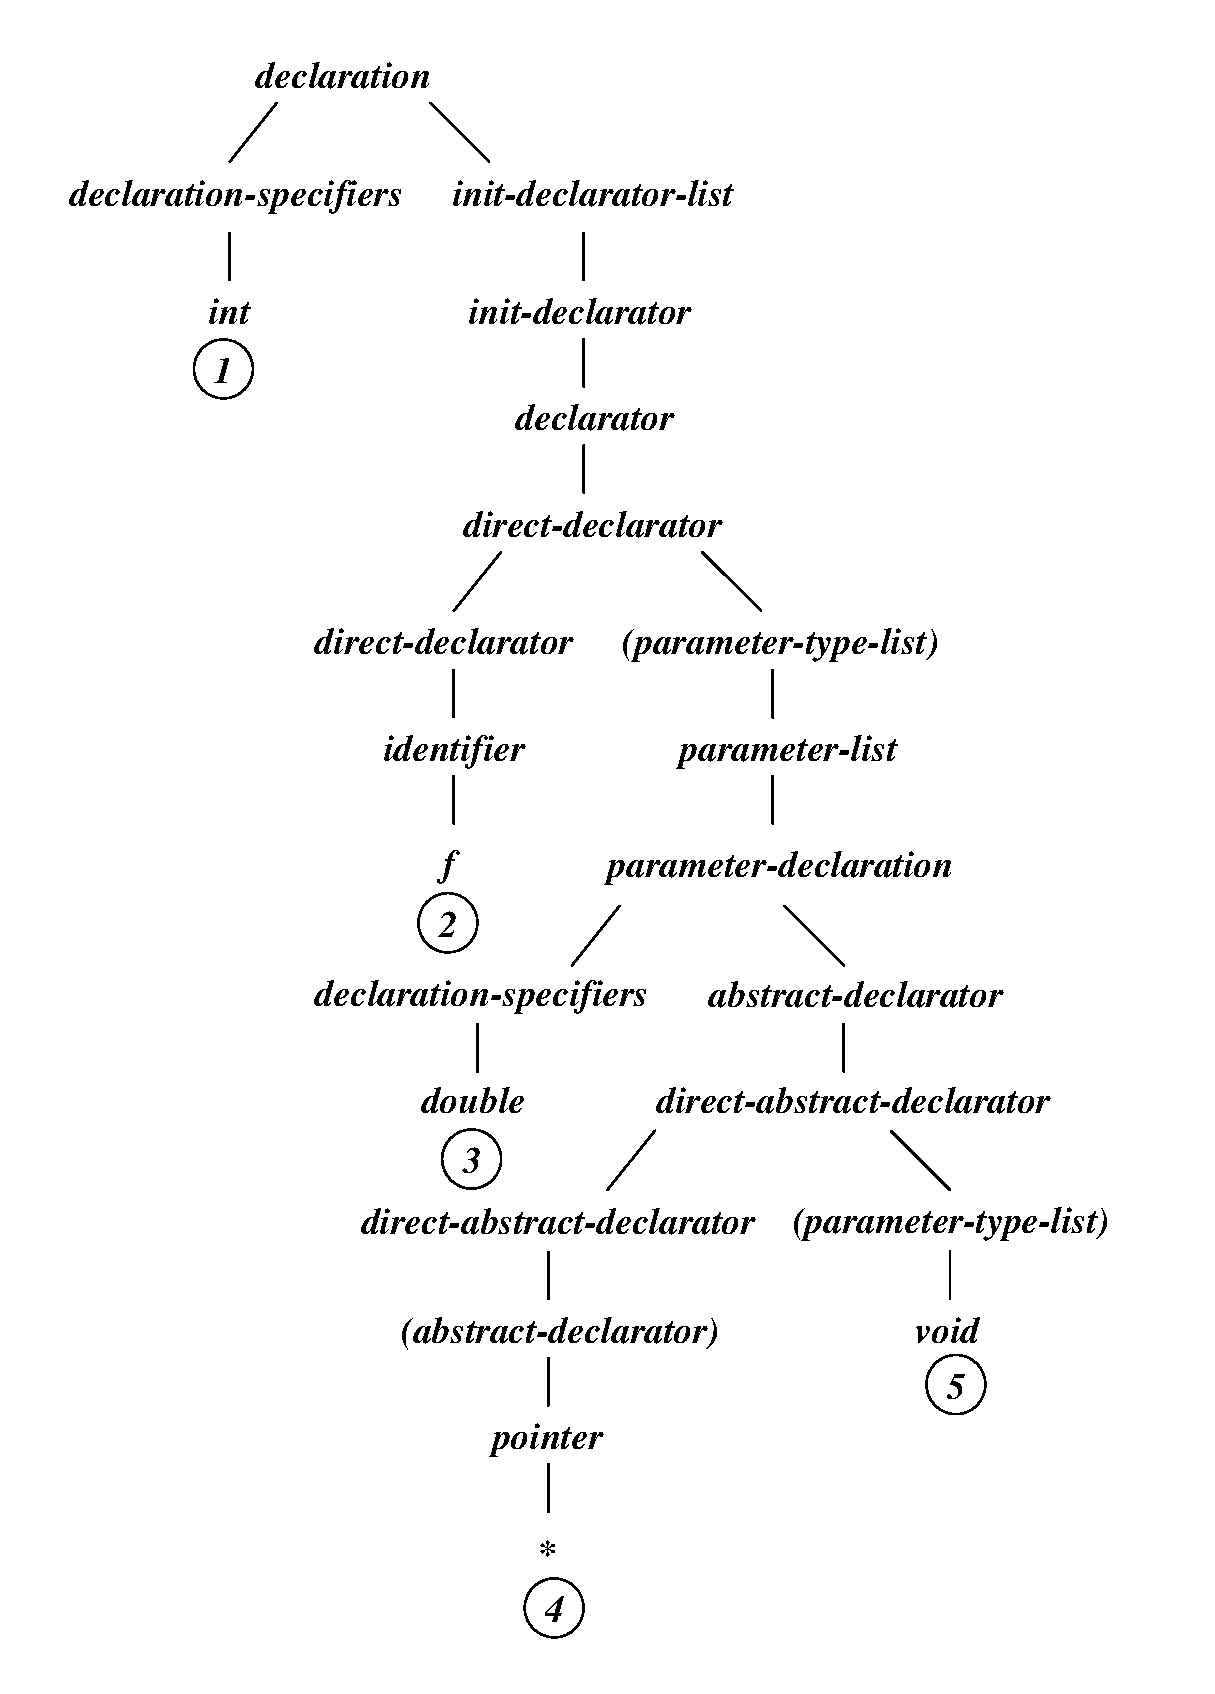
\includegraphics[width=1.0125\linewidth,height=1.4175\linewidth]{decl001.eps}
\end{latexonly}
\caption{syntax tree of {\tt{int f(double (*)(void));}}}
\label{decl_e001}
\end{center}
\end{figure}
Circled numbers in figure \ref{decl_e001} are reducing order
while bottom-up parsing. Frontend adds the entry according to `{\tt{f}}'
for this declaration, and the type attribute of this entry becomes
like figurue \ref{decl_e002}

\begin{figure}[htbp]
\begin{center}
\begin{htmlonly}
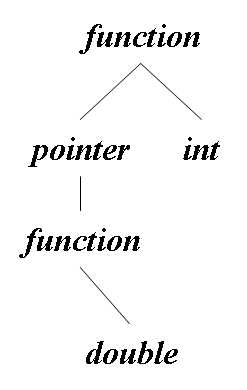
\includegraphics[width=0.5\linewidth,height=0.6\linewidth]{decl002.png}
\end{htmlonly} 
\begin{latexonly}
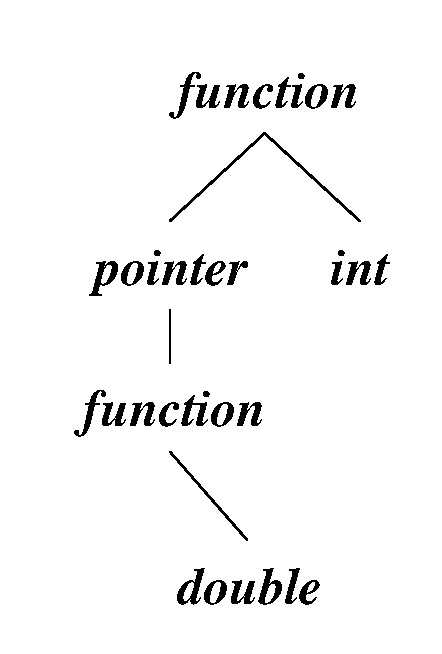
\includegraphics[width=0.5\linewidth,height=0.6\linewidth]{decl002.eps}
\end{latexonly}
\caption{{\em type expression} of {\tt{int f(double (*)(void));}}}
\label{decl_e002}
\end{center}
\end{figure}

Please note that when grammer symbol {\tt{pointer}} is reduced, frontend 
must create {\em type expression} ``pointer to $x$'',
and later, frontend must replace $x$ to {\em type expression} 
``function returing {\tt{double}} whick does not take argument''.

The reason of later replacing is that
grammer symbol {\tt{pointer}} is reduced
 (${\MARU{\tt 4}}$ on figure \ref{decl_e001})
and then {\tt{void}} or grammer symbol {\tt{parameter-type-list}} 
is reduced(${\MARU{\tt 5}}$ on figure \ref{decl_e001}).

Second, we'll think about below declaration, specifically.
\begin{verbatim}
int (*a[])();
\end{verbatim}
Figure \ref{decl_e003} shows syntax tree of this declaration
and circled numbers in figure \ref{decl_e003} are reducing order
while bottom-up parsing, samely.
\begin{figure}[htbp]
\begin{center}
\begin{htmlonly}
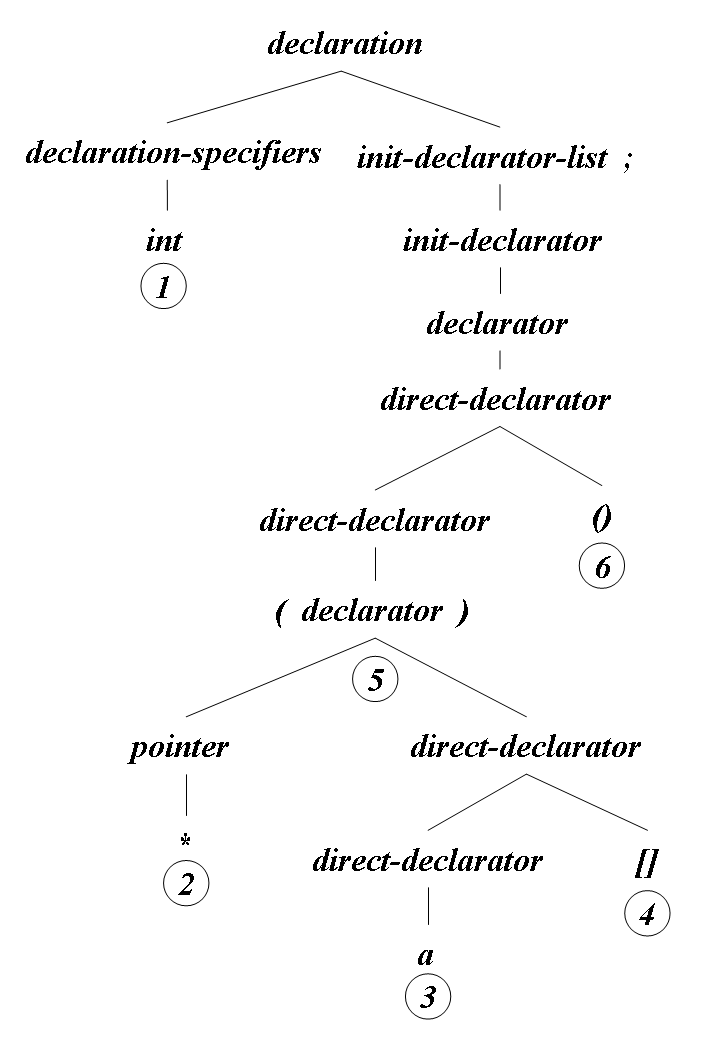
\includegraphics[width=1.0125\linewidth,height=1.4175\linewidth]{decl003.png}
\end{htmlonly} 
\begin{latexonly}
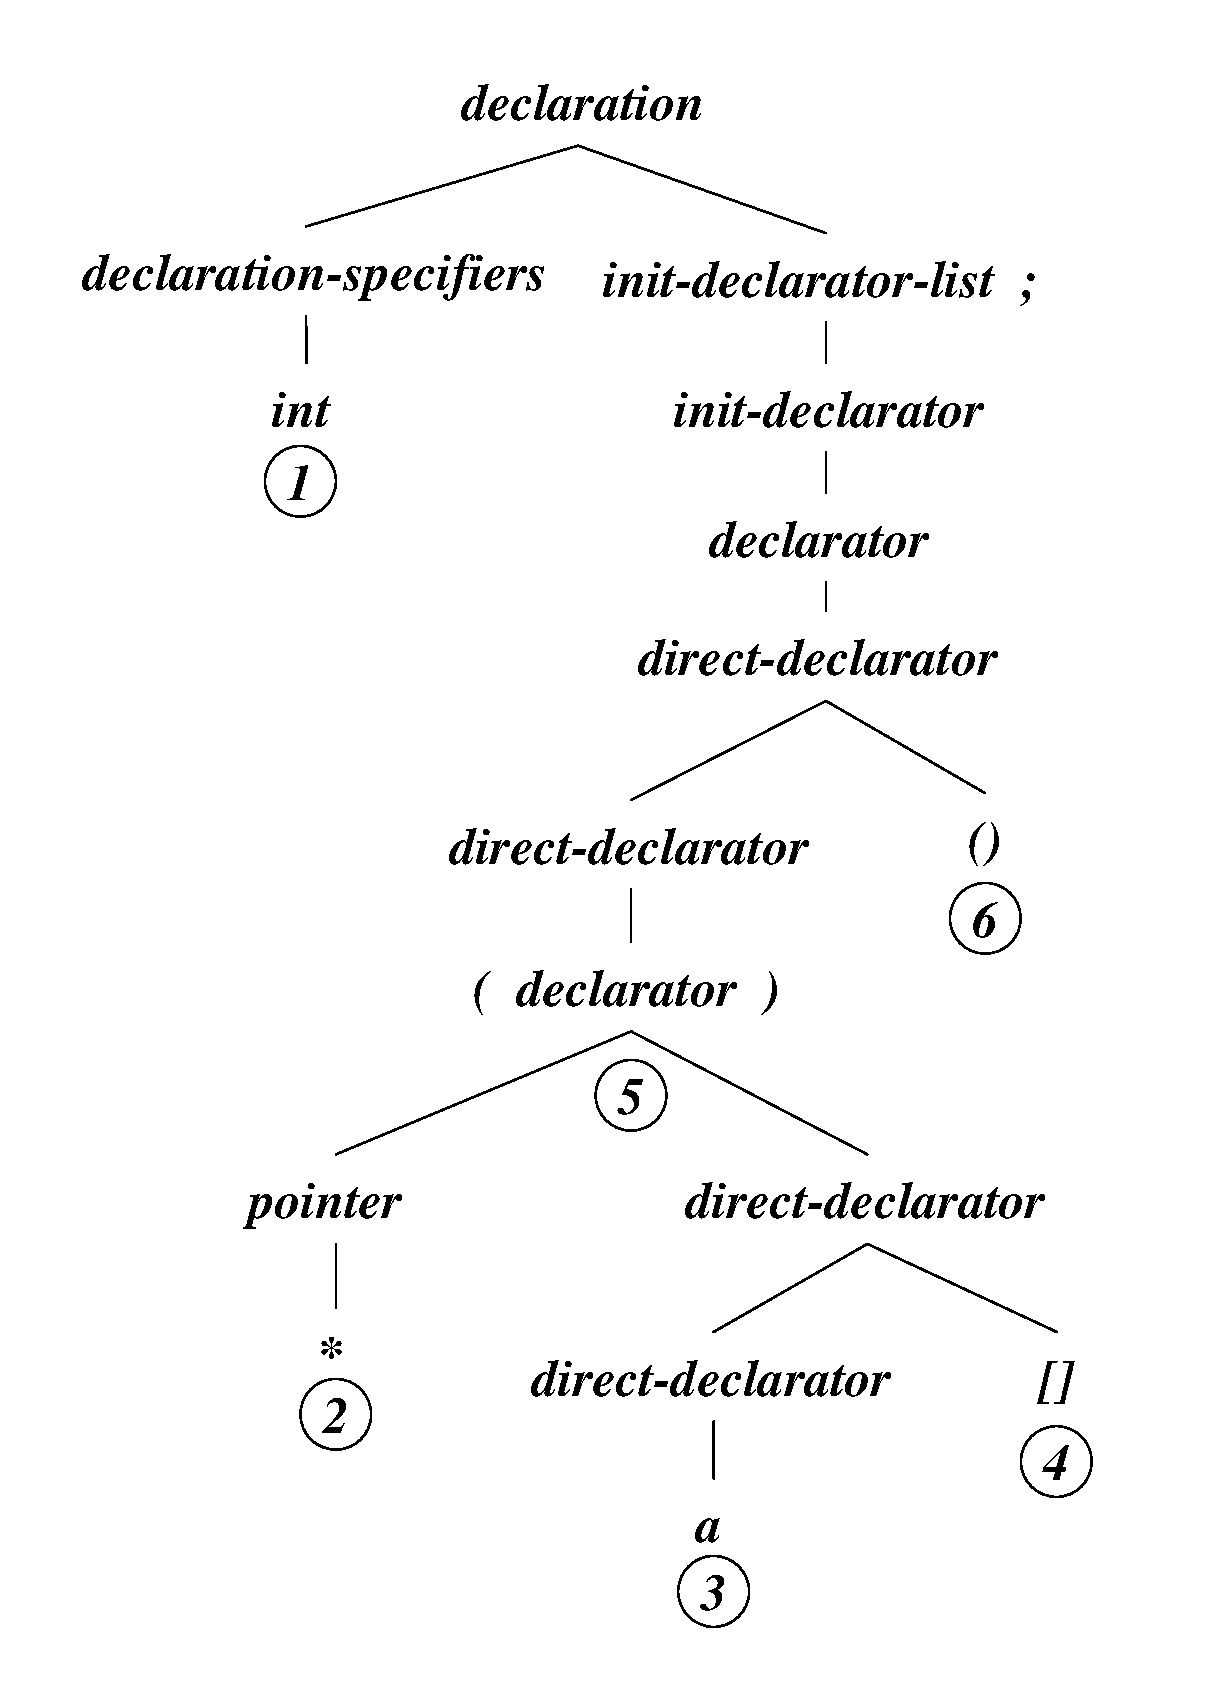
\includegraphics[width=1.0125\linewidth,height=1.4175\linewidth]{decl003.eps}
\end{latexonly}
\caption{syntax tree of {tt{int (*a[])()}}}
\label{decl_e003}
\end{center}
\end{figure}
 Frontend adds the entry according to `{\tt{a}}'
for this declaration, and the type attribute of this entry becomes
like figurue \ref{decl_e004}
\begin{figure}[htbp]
\begin{center}
\begin{htmlonly}
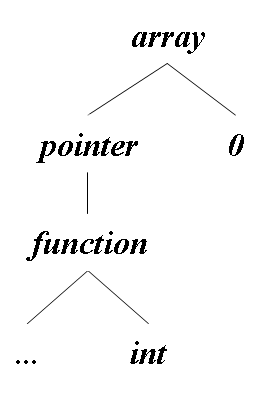
\includegraphics[width=0.5\linewidth,height=0.6\linewidth]{decl004.png}
\end{htmlonly} 
\begin{latexonly}
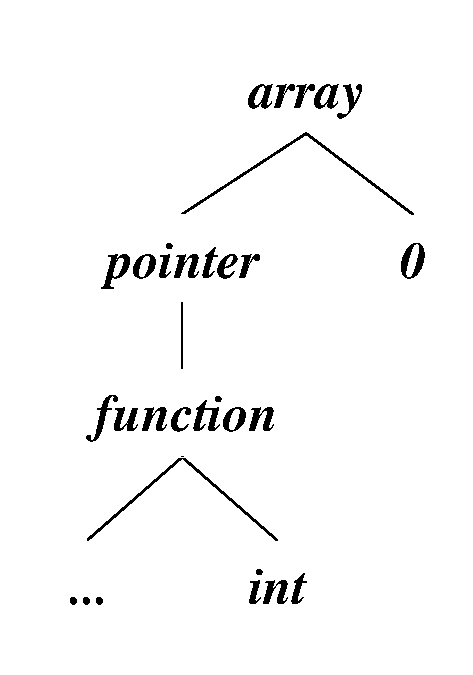
\includegraphics[width=0.5\linewidth,height=0.6\linewidth]{decl004.eps}
\end{latexonly}
\caption{{\em type expression} of {\tt{int (*a[])();}}}
\label{decl_e004}
\end{center}
\end{figure}

At ${\MARU{\tt 5}}$ on figure \ref{decl_e003}
\begin{verbatim}
declarator : pointer direct-declarator
\end{verbatim}
Above grammer is reduced. In this point, frontned calcurates
the type attribute of {\tt{declarator}} like below:

The type attribute of grammer symbol {\tt{pointer}} 
is ``pointer to $x$'', and that of grammer symbol
{\tt{direct-declarator}} is ``array of $y$''.
Now, $y$ is replaced to ``point to $x$'',
then, that of {\tt{declarator}} becomes
``array of pointer to $x$''.

And more, at ${\MARU{\tt 6}}$ on figure \ref{decl_e003}
\begin{verbatim}
direct-declarator : direct-declarator ()
\end{verbatim}
Above grammer is reduced. In this point, frontned calcurates
the type attribute of {\tt{direct-declarator}} like below:

The type attribute of right hand grammer symbol {\tt{direct-declarator}}
is ``array of pointer to $x$''.
Now, $x$ is replaced to ``function returing $z$'',
then, that of {\tt{direct-declarator}} becomes
``array of pointer to function returning $z$''.

Here, please remeber that if below grammer
\begin{verbatim}
direct-declarator : direct-declarator [ ]
\end{verbatim}
is reduced, the type attribute of left hand doesn't always become
array. And samely, if below grammer
\begin{verbatim}
direct-declarator : direct-declarator ( )
\end{verbatim}
is reduced, the type attribute of left hand doesn't always become
function.
Below declarations
\begin{verbatim}
int f()[];
int a[]();
\end{verbatim}
are error in C language, but we'll show how to calcurate
{\em type expression}. 

\begin{tabular}{cccccl}
           & {\tt{f}} &           &           &    &
                 type of {\tt{f}} is $x$                       \\
           & {\tt{f}} & {\tt{()}} &           &    &
                 type of {\tt{f}} is ``function returing $x$'' \\
           & {\tt{f}} & {\tt{()}} & {\tt{[]}} &    &
                 type of {\tt{f}} is ``function returning array of $x$'' \\
{\tt{int}} & {\tt{f}} & {\tt{()}} & {\tt{[]}} &    &
            type of {\tt{f}} is ``function returning array of {\tt{int}}'' \\
           &          &           &           &    &
                                                         \\
           & {\tt{a}} &           &           &    &
                 type of {\tt{a}} is $x$                       \\
           & {\tt{a}} & {\tt{[]}} &           &    &
                 type of {\tt{a}} is ``array of $x$'' \\
           & {\tt{a}} & {\tt{[]}} & {\tt{()}} &    &
            type of {\tt{a}} is ``array of function returing $x$'' \\
{\tt{int}} & {\tt{a}} & {\tt{[]}} & {\tt{()}} &    &
            type of {\tt{a}} is ``array of function returing {\tt{int}}'' \\
\end{tabular}

\begin{QandA}
When calcurating type expression from C language declaration,
type $x$ is replaced to type $y$. But is it necessary in different sense to
replace
some type to another type for calcurating type expression
from below declarations?

\begin{verbatim}
typedef int A[10];
const A a;  /* incorrect : const(array(int,10)) */
            /* correct : array(const(int),10) */

typedef int* pi;
const pi cpi;  /* correct : const(pointer(int)) */
               /* incorrect : pointer(const(int)) */
\end{verbatim}

Answer : Yes. In the different sense, it is necesssary
to replace because type qualifier
 {\tt{const}}, {\tt{volatile}}, {\tt{restrict}}
cannot qualify array or function type.
\end{QandA}

\section{Initializer}
\label{decl_e005}
Initializer is a part of declaration.
Not only it specifies the values of declared variable, but also
decides the type if declared variable has incomplete array type.
For example,
\begin{verbatim}
int a;
...
{
  int a[] = { sizeof a };  /* error : a[0] is not sizoef(int) */

  int b[] = { 0, 1, 2 };  /* int b[3]  */
}
\end{verbatim}
As described in \ref{lex_yacc_e004},
when compiler detects the minimum unit of declaration,
compiler must insert it into symbol table.

In this section, we'll think about the way to recognize
initializer. The following infomation is updated
while recognizing initializer.
\begin{itemize}
\item Initialized object type $T$
\item Set of initial value $V$, whose element is pair of offset and value.
\item Offset and max value of it $({\delta},{\delta}_{\tt{max}})$
\item The order and max value of it $(n,n_{\tt{max}})$.
      $n$ means the order in {\tt{initializer-list}} for initialized
      object type $T$.
\item The order and length of {\tt{initializer-list}} $(m,M)$.
      $m$ doesn't depend on initialized object type $T$,
      $m$ just means the position
      at {\tt{initializer-list}}. 
\end{itemize}
This infomation is denoted like below pair
\[
I \equiv (T,V,({\delta},{\delta}_{\tt{max}}),(n,n_{\tt{max}}),(m,M)) 
\]
And if we want to refer about $\delta_{\max}$ of $I$, we'll
use  $I.\delta_{\max}$ notation.

\begin{quotation}
{\bf Algorithm for initializer}
\begin{description}
When the token {\tt{=}} which is followed by
grammer symbol {\tt{initializer}} is reduced,
apply below {\bf procedure for initializer} for
\[
I \equiv (T,V,(0,0),(-1,-1),(-1,-1))
\]
where, $T$ is the type of initialized variable
which is specified {\tt{= initializer}}.
$V$ is empty set. And $-1$ denotes that
frontend doesn't work for {\tt{initializer-list}}.

\item[procedure for initializer]

\

If {\tt{initializer}} is reduced from {\tt{assignmet-expression}},
apply {\bf procedure for assignmet-expression} for input of this
procedure $I$. Otherwise apply for
{\bf procedure for initializer-list} for $I$.




\item[procedure for assignmet-expression]

\

\begin{enumerate}
\item Calcurate value of {\tt assignment-expression}. Let $y$ denote
      the value. 
\item \label{initializer010}
      If this initialization is charcter array initialization,
      do it, and terminate this procedure.
\item \label{initializer004}
      If $I.n \ge 0$, get $I.n$ th offset (${\delta}'$) and type ($T'$)
      for initialized object type $I.T$.
      If $T'$ is not scalar type and the type of $y$ is scalar type,
      apply below {\bf procedure for assignment-expression special case}
      for $I$. And terminate this procedure. 
\item If not, i.e. $I.n < 0$,
      ${\delta}' = I.\delta$ , $T' = I.T$.
\item Judge assignment $y$ to $T'$. If it is not valid, this
      initialization is error. Terminate this procedure.
\item If it is necessary to cast $y$ with type $T'$,
      let $y'$ the result of cast.
\item Insert $({\delta}', y')$ into $I.V$.
\item $I.\delta = {\delta}' + {\tt sizeof}(T')$,
      ${I.\delta}_{\tt{max}} = \max({I.\delta}_{\tt{max}}, I.{\delta})$.
\item If $I.n \ge 0$ , $I.n = I.n + 1$,
       $I.n_{\tt{max}} = \max(I.n_{\tt{max}}, I.n)$.
\end{enumerate}

\item[procedure for assignment-expression special case]

\

\begin{enumerate}
      \item
      Get $I.n$ th offset (${\delta}'$) and type ($T'$)
      for initialized object type $I.T$.

      \item
      Apply again {\bf procedure for assignment-expresion} for
\begin{eqnarray*}
I' & \equiv & (T',V',(\hat{\delta},\hat{\delta}),(n',n'),(I.m,I.M)) \\
\hat{\delta} & \equiv & I.\delta \, \verb|%|\,{\tt{sizeof}}(T') \\
n' & \equiv &\left\{ \begin{array}{l}
\hat{\delta}\,\,/\,\,{\tt{sizeof}}(\hat{T})
{\mbox{ if }}T'{\mbox{ is array of }}\hat{T} \\
{\mbox{The order of the member }} x {\mbox{ in }} T' \\
{\mbox{ if }}T'{\mbox{ is structure or union, let }} x 
{\mbox{ member of }} T' \\
{\mbox{ whose offset is }}  \hat{\delta}
\end{array} \right.
\end{eqnarray*}
      where $V'$ is empty set of initial value.
      \item \label{initializer008}
      Apply {\bf procedure zero initialization} for $I'$.
      \item  \label{initializer011}
      Copy $V'$ to $I.V$ with adding offset $\delta'$.
      \item  \label{initializer012}
      If $T'$ is array type and the dimension is equal to $n'$, 
      or if $T'$ is structure or union and the number of member
      is equal to $n'$, increment $I.n$,
      $I.n_{\tt{max}} = \max(I.n_{\tt{max}}, I.n)$, $I'.\delta = 0$
      \item $I.\delta = I.\delta + {\tt{sizeof}(T')}* I.n + I'.\delta$,
      $I.\delta_{\max} = \max(I.\delta_{\max}, I.\delta)$. 
\end{enumerate}

\item[procedure zero initialization]

\

\begin{enumerate}
\item If $I.m < 0$ or $I.m \ne I.M$, i.e.
      it is not the end of {\tt{initializer-list}},
      terminate this procedure.

\item If $I.\delta_{\tt{max}} = {\tt sizeof}(I.T)$, i.e.
      all are initialized, teminate this procedure.

\item Initialized object type $I.T$ is incomplete array type,
      teminate this procedure.

\item \label{initializer014} 
      Get $I.n_{\max}$ th offset and type. If not, terminate
      this procedure.

\item Update $I.\delta$ to offset at \ref{initializer014},
      $I.\delta_{\max} = {\max}({I.\delta}_{\max},I.{\delta})$.

\item Type $T'$ at \ref{initializer014} is scalar type,
      add $(I.\delta,z)$ into $I.V$, where $z$ is the result of
      cast $0$ to $T'$.
      $I.\delta = I.\delta + {\tt{sizeof}}(T')$,
       $I.\delta_{\max} = {\max}(I.{\delta}_{\max},I.{\delta})$.

\item Otherwise, i.e. type $T'$ at \ref{initializer014} is not scalar
      type, apply {\bf procedure zero initialization} for
\[
 I' \equiv (T',V',(0,0),(0,0),(0,0))
\]
And copy $V'$ to $V$ with adding offset $I.\delta$.
$I.\delta = I.\delta + I'.{\delta_{\max}}$,
$I.\delta_{\max} = {\max}(I.\delta_{\max},I.\delta)$.

\item $I.n_{\max} = I.n_{\max} + 1$, $I.n = I.n_{\max}$,
Go to \ref{initializer014}.
\end{enumerate}


\item[procedure for initializer-list]

\

\begin{enumerate}
\item \label{initializer005}
      If $I.n \ge 0$, get $I.n$ th offset ${\delta}'$ and
      type $T'$ for initialized object type $I.T$.
      If $I.n < 0$, ${\delta}' = I.{\delta}$, $T' = I.T$.
\item An empty initial value set $V'$ and the length of
      {\tt{initializer-list}} $M$,
\[
 I' \equiv (T',V',(0,0),(0,0),(0,M))
\]
Apply below for $I'$

\item \label{initializer009}

For each element of {\tt{initializer-list}}
\begin{enumerate}
\item If {\tt{designation}} exists,
      apply {\bf procedure for desination}, and go to \ref{initializer009}.
\item Otherwise apply {\bf procedure for initializer} for $I'$.
\end{enumerate}

\item \label{initializer006}
      Apply {\bf procedure zero initialization} for $I'$.

\item Copy $V'$ to $I.V$ with adding offset ${\delta}'$.

\item If $I.n \ge 0$,
$I.n = I.n + 1$, $I.n_{\max} = \max(I.n_{\max},I.n)$.

\item $I.\delta = {\delta}' + I'.{\delta}_{\max}$,
      $I.\delta_{\tt{max}} = {\max}(I.\delta_{\tt{max}},\delta)$.

\item $I'.m = I.m + 1$.

\end{enumerate}

\item[procedure for designation]

\

\begin{enumerate}
\item Let $T' = I.T$, and $V'$ is an empty initial value set.
For each element of  {\tt{designation}},
apply 
below {\bf procedure for designator} for
\[
 I' \equiv (T',V',(0,0),(-1,-1),(-1,-1))
\]

\item Erase elements whose offset is less than $I.{\delta}_{\max}$
from $V'$. 

\item Copy $V'$ to $I.V$.

\item $I.n = I'.n + 1$, $I.n = {\max}(I.n_{\max},I.n)$.

\item $I.m = I.m + 1$.

\item Let $T'' = T'$, and $V''$ is an empty initial value set.
Apply  {\bf procedure for initializer} for
\[
 I'' \equiv (T'', V'', (0,0),(-1,-1),(I.m,I.M))
\]

\item Copy $V''$ to $I.V$ with adding offset $I'.{\delta}$.

\item $I.{\delta} = I'.{\delta} + I''.{\delta}$, 
      $I.{\delta}_{\max} = {\max}(I.{\delta}_{\max},I.\delta)$.

\item If $I.T$ is incomplete array type, let $E$ denote element type of
      the array type.
      If ${\tt{sizeof}(E)}\,\verb|%|\,I.\delta_{\max}$ is not equal to $0$,
      Let $T'''$ to be array of $E$ whose dimension is $s /
      I.\delta_{\max} + 1$.
      Otherwise, $T''' = I.T$.
      
\item \label{initializer015}
Let $V'''$ to be an empty initial value set.
Apply {\bf procedure zero initialization} for
\[
 I''' \equiv (T''',V''',0,0,0,0,I.m,I.M)
\]

\item Erase elements whose offset is less than $I.{\delta}_{\max}$
from $V'''$. 

\item Copy $V'''$ to $I.V$.

\item If $I'''.\delta > 0$,
$I.\delta = I'''.\delta$,
$I.\delta_{\max} = \max(I.\delta_{\max},I.\delta)$.

\end{enumerate}

\item[procedure for designator]

\

If the {\tt{designator}} is subscripting designator,
apply below {\bf procedure for subscripting designator}.
Otherwise apply below {\bf procedure for member designator}.

\item[procedure for subscripting designator]

\

\begin{enumerate}
\item If the initialized object type is not array, make it error.
      Otherwise let $A$ denote the array type.
\item Get the subscripting value. If it is not integer constant,
      make it error. Otherwise let $n'$ denote the value.
\item Let $T'$ denote the array of the type which is the element type of
      $A$, and whose dimension is $n'$. And let $V'$ denote an empty
      initial value set. For

\[
 I' \equiv (T',V',0,0,0,0,0,0) 
\]
apply {\bf procedure zero initialization}.

\item Copy $V'$ to $I.V$ with adding offset $I.\delta$.

\item Update $I.T$ to the element type of $A$.
\item $I.\delta = I.\delta + I'.{\delta_{\max}}$,  
      $I.{\delta_{\max}} = {\max}(I.{\delta_{\max}},I.\delta)$.
\item $I.n = I'.n_{\max}$,
      $I.n_{\max} = {\max}(I.n_{\max},I.n)$.
\end{enumerate}

\item[procedure for member designator]

\

\begin{enumerate}
\item If the unqualified initialized object type is neither
      structure nor union, make it error. Otherwise
      let $R$ denote the type.
\item If $R$ doesn't contain the member, make it error.
      Otherwise let ${\delta}'$ and $T'$ denote the member offset
      and the type of member, respectively. Let $n'$
      denote the order of member in $R$.
\item Let $V'$ denote an empty
      initial value set. For
\[
 I' \equiv (R,V',0,0,0,0,0,0)
\]
apply {\bf procedure zero initialization}.

\item Erase elements whose offset is less than ${\delta}'$
from $V'$. 

\item Copy $V'$ to $I.V$ with adding offset $I.\delta$.

\item Update $I.T$ to be $T'$.
\item $I.\delta = I.\delta + \delta'$,
      $I.{\delta_{\max}} = {\max}(I.{\delta_{\max}},I.{\delta})$.
\item $I.n = n'$, $I.n_{\max} = \max(I.n_{\max},I.n)$.
\end{enumerate}

\end{description}
\end{quotation}

If the initializer is specified to static variable,
all value of the element of the initial value set must be 
constant or address of some variable or function.
Otherwise, frontend generates 3 address code
{\tt{x}}[$\delta$] := $y$, 
for each element $(\delta,y)$ of the initial value set.

In the below examples, we'll investigate how the algorithm
works. For easy, assume that {\tt{sizeof(int)}} is equalt to 4,
 {\tt{sizeof(double)}} is equal to 8, and the alignment in 
structure is 4, 8, respectively.

\begin{Example}
\label{initializer000}
{{\tt int a \Rubyt{=}{\MARU{\tt 1}} 1;}}

\noindent
At $\MARU{\tt 1}$, for
\[
I \equiv ({\tt{int}},V,(0,0),(-1,-1),(-1,-1))
\]
apply the algorithm. Initializer {\tt 1}
is {\tt assignment-expression}, so,
apply  {\bf procedure for assignmet-expression} for $I$.
The value and type of \\
{\tt assignment-expression} is $1$ and {\tt{int}},
respectively, and assignment is valid for $I.T = {\tt{int}}$.
The result of the algorithm is
\begin{eqnarray*}
I & = & ({\tt{int}},V,(4,4),(-1,-1),(-1,-1)) \\
V & = & \{(0,1)\}
\end{eqnarray*}
\end{Example}

\begin{Example}
\label{initializer001}
{{\tt int a \Rubyt{=}{\MARU{\tt 1}}\Rubyt{\{}{\MARU{\tt 2}}
\Rubyt{2}{\MARU{\tt 3}}
\Rubyt{\}}{\MARU{\tt 4}};}}

\noindent
At $\MARU{\tt 1}$, for
\[
I_0 \equiv ({\tt{int}},V_0,(0,0),(-1,-1),(-1,-1))
\]
apply the algorithm. 
Initializer {\tt \{ 2 \}}
is {\tt initializer-list}, so, apply
 {\bf procedure for initializer-list} for $I$.

\noindent
At $\MARU{\tt 2}$, for
\[
I_1 \equiv ({\tt{int}},V_1,(0,0),(0,0),(0,1))
\]
apply {\bf procedure for initializer-list} \ref{initializer009}.

\noindent
At $\MARU{\tt 3}$, {\bf procedure for assignmet-expression}
\ref{initializer004} judges that 
{\tt{0}}th offset and type for {\tt{int}} is $(0,{\tt{int}})$. 
After $\MARU{\tt 3}$, the result is
\begin{eqnarray*}
I_1 & = & ({\tt{int}},V_1,(4,4),(1,1),(1,1)) \\
V_1 & = & \{(0,2)\}
\end{eqnarray*}

\noindent
At $\MARU{\tt 4}$,
copy $V_1$ to  $V_0$ with adding offset $I_1.\delta = 0$.
After $\MARU{\tt 4}$, the result is
\begin{eqnarray*}
I_0 & = & ({\tt{int}},V_1,(4,4),(-1,-1),(-1,-1)) \\
V_0 & = & \{(0,2)\}
\end{eqnarray*}
\end{Example}

\begin{Example}
\label{initializer002}
{\tt int a[] \Rubyt{=}{\MARU{\tt 1}} 
\Rubyt{\{}{\MARU{\tt 2}}
\Rubyt{1}{\MARU{\tt 3}},
\Rubyt{2}{\MARU{\tt 4}},
\Rubyt{3}{\MARU{\tt 5}}
\Rubyt{\}}{\MARU{\tt 6}}
;}

\noindent
At $\MARU{\tt 1}$, for
\[
I_0 \equiv ({\tt int\,\,[]}, V_0, (0,0),(-1,-1),(-1,-1))
\]
apply the algorithm.

\noindent
At $\MARU{\tt 2}$, for
\[
I_1 \equiv ({\tt int\,\,[]}, V_1, (0,0),(0,0),(0,3))
\]
apply {\bf procedure for initializer-list} \ref{initializer009}.

\noindent
At $\MARU{\tt 3}$ , $\MARU{\tt 4}$ , $\MARU{\tt 5}$,
{\bf procedure for assignmet-expression} \ref{initializer004} 
judges that {\tt{0}}th, {\tt{1}}st and {\tt{2}}nd
offset and type for {\tt int []} is 
{\tt (0,int)}, {\tt (4,int)} and {\tt (8,int)}, respectively.
So, insert {\tt (0,1)}, {\tt (4,2)} and {\tt (8,3)} into $V_1$ respectively.
After $\MARU{\tt 5}$, the result is
\begin{eqnarray*}
I_1 & = & ({\tt{int\,\,[]}},V_1,(12,12),(3,3),(3,3)) \\
V_1 & = & \{(0,1), (4,2), (8,3)\}
\end{eqnarray*}

\noindent
At $\MARU{\tt 6}$, copy $V_1$ to  $V_0$ with adding offset $0$.
After $\MARU{\tt 6}$, the result is
\begin{eqnarray*}
I_0 & = & ({\tt{int\,\,[]}},V_0,(12,12),(-1,-1),(-1,-1)) \\
V_0 & = & \{(0,1), (4,2), (8,3)\}
\end{eqnarray*}
\end{Example}

After applying the algorithm, frontend changes the type of
{\tt{a}} from {\tt{int []}} to {\tt{int [3]}}.

\begin{Example}
{\tt int a[]
\Rubyt{=}{\MARU{\tt 1}}
\Rubyt{1}{\MARU{\tt 2}}
;
}

\noindent
At $\MARU{\tt 1}$, for
\[
I \equiv ({\tt{int\,\,[]}},V,(0,0),(-1,-1),(-1,-1)) 
\]
apply the algorithm.

\noindent
At $\MARU{\tt 2}$, {\bf procedure for assignmet-expression}
 \ref{initializer004} sets $0$ to ${\delta}'$ and 
{\tt{int []}} to $T'$ because  
$n = -1$. So the initialized object type is {\tt int []},
the assignment is not valid, it's error.
\end{Example}

\begin{Example}

\

{\tt struct S \{ int a; int b; \};}

{\tt struct S s \Rubyt{=}{\MARU{\tt 1}}
\Rubyt{\{}{\MARU{\tt 2}}
\Rubyt{1}{\MARU{\tt 3}},
\Rubyt{2}{\MARU{\tt 4}}
\Rubyt{\}}{\MARU{\tt 5}};
}

\noindent
At $\MARU{\tt 1}$, for
\[
I_0 \equiv ({\tt{struct\,\,S}},V_0,(0,0),(-1,-1),(-1,-1)) 
\]
apply the algorithm.

\noindent
At $\MARU{\tt 2}$, for
\[
I_1 \equiv ({\tt{struct\,\,S}},V_1,(0,0),(0,0),(0,2))
\]
apply {\bf procedure for initializer-list} \ref{initializer009}.


\noindent
At $\MARU{\tt 3}$, $\MARU{\tt 4}$,
{\bf procedure for assignmet-expression}
 \ref{initializer004} judges that
{\tt{0}}th, {\tt{1}}st 
offset and type for {\tt struct S} is 
{\tt (0,int)}, {\tt (4,int)},  respectively.
Insert {\tt (0,1), (4,2)} into $V_1$, respectively.
After $\MARU{\tt 4}$, the result is
\begin{eqnarray*}
I_1 & = & ({\tt{struct\,\,S}},V_1,(8,8),(2,2),(2,2)) \\
V_1 & = & \{(0,1), (4,2)\}
\end{eqnarray*}

\noindent
At $\MARU{\tt 5}$,
copy $V_1$ to $V_0$ with adding offset $0$.
After $\MARU{\tt 5}$, the result is
\begin{eqnarray*}
I_0 & = & ({\tt{struct\,\,S}},V_0,(8,8),(-1,-1),(-1,-1)) \\
V_0 & = & \{(0,1), (4,2)\}
\end{eqnarray*}
\end{Example}

\begin{Example}

\

{\tt struct S \{ int a; char b[5]; double c;\};}

{\tt struct S s \Rubyt{=}{\MARU{\tt 1}} 
\Rubyt{\{}{\MARU{\tt 2}}
\Rubyt{1}{\MARU{\tt 3}},
\Rubyt{"foo"}{\MARU{\tt 4}},
\Rubyt{2.0}{\MARU{\tt 5}}
\Rubyt{\}}{\MARU{\tt 6}};
}

\noindent
At $\MARU{\tt 1}$, for
\[
I_0 \equiv ({\tt{struct\,\,S}},V_0,(0,0),(-1,-1),(-1,-1)) 
\]
apply the algorithm.

\noindent
At $\MARU{\tt 2}$, for
\[
I_1 \equiv ({\tt{struct\,\,S}},V_1,(0,0),(0,0),(0,3))
\]
apply {\bf procedure for initializer-list} \ref{initializer009}.

\noindent
At $\MARU{\tt 3}$,
{\bf procedure for assignmet-expression} \ref{initializer004} judges
that 
{\tt{0}}th offset and type for {\tt{struct S}} is $(0,{\tt{int}})$.
Insert {\tt (0,1)} into $V_1$. After $\MARU{\tt 3}$, the result is
\begin{eqnarray*}
I_1 & = & ({\tt{struct\,\,S}},V_1,(4,4),(1,1),(1,3)) \\
V_1 & = & \{(0,1)\}
\end{eqnarray*}

\noindent
At $\MARU{\tt 4}$,
{\bf procedure for assignmet-expression} \ref{initializer004} judges
that
{\tt{1}}st offset and type for {\tt{struct S}} is $(4,{\tt{char\,\,[5]}})$.
Insert {\tt{(4,'f')}},
{\tt{(5,'o')}},
{\tt{(6,'o')}},
{\tt{(7,'\verb|\|0')}},
{\tt{(8,'\verb|\|0')}}
into $V_1$.
After $\MARU{\tt 4}$, the result is
\begin{eqnarray*}
I_1 & = & ({\tt{struct\,\,S}},V_1,(9,9),(2,2),(2,3)) \\
V_1 & = & \{(0,1),
 (4,{\tt{'f'}}),(5,{\tt{'o'}}),(6,{\tt{'o'}}),(7,'\verb|\|0'),(8,'\verb|\|0')\}
\end{eqnarray*}

\noindent
At $\MARU{\tt 5}$,
{\bf procedure for assignmet-expression} \ref{initializer004} judges
that
{\tt{2}}nd offset and type for {\tt{struct S}} is $(16,{\tt{double}})$.
Insert {\tt (16,2.0)} into $V_1$.
After $\MARU{\tt 5}$, the result is
\begin{eqnarray*}
I_1 & = & ({\tt{struct\,\,S}},V_1,(24,24),(3,3),(3,3)) \\
V_1 & = & \{(0,1),
 (4,{\tt{'f'}}),(5,{\tt{'o'}}),(6,{\tt{'o'}}),(7,'\verb|\|0'),(8,'\verb|\|0'),
(16,2.0)\}
\end{eqnarray*}

\noindent
At $\MARU{\tt 6}$, copy $V_1$ to $V_0$ with adding offset {\tt 0}.
After $\MARU{\tt 6}$, the result is
\begin{eqnarray*}
I_0 & = & ({\tt{struct\,\,S}},V_0,(24,24),(-1,-1),(-1,-1)) \\
V_0 & = & \{(0,1),
 (4,{\tt{'f'}}),(5,{\tt{'o'}}),(6,{\tt{'o'}}),(7,'\verb|\|0'),(8,'\verb|\|0'),
(16,2.0)\}
\end{eqnarray*}

\end{Example}

\begin{Example}

\

{\tt struct S \{ int a; double b; char c[5];\};}

{\tt struct S s \Rubyt{=}{\MARU{\tt 1}}}
{\tt \Rubyt{\{}{\MARU{\tt 2}}}

{\tt \Rubyt{\{}{\MARU{\tt 3}}}
{\tt \Rubyt{2}{\MARU{\tt 4}}}
{\tt \Rubyt{\}}{\MARU{\tt 5}},}
{\tt \Rubyt{\{}{\MARU{\tt 6}}}
{\tt \Rubyt{3.0}{\MARU{\tt 7}}}
{\tt \Rubyt{\}}{\MARU{\tt 8}},}
{\tt \Rubyt{\{}{\MARU{\tt 9}}}
{\tt  \Rubyt{"foo"}{\MARU{\tt 10}}}
{\tt \Rubyt{\}}{\MARU{\tt 11}}}

{\tt \Rubyt{\}}{\MARU{\tt 12}};}

\noindent
At $\MARU{{\tt 1}}$, for
\[
I_0 \equiv ({\tt{struct\,\,S}},V_0,(0,0),(-1,-1),(-1,-1))
\]
apply the algorithm.

\noindent
At $\MARU{{\tt 2}}$, for
\[
I_1 \equiv ({\tt{struct\,\,S}},V_1,(0,0),(0,0),(0,3))
\]
apply {\bf procedure for initializer-list} \ref{initializer009}.

\noindent
At $\MARU{{\tt 3}}$, because $I_1.n = 0$,
{\bf procedure for initializer-list}
\ref{initializer005} judges that
{\tt{0}}th offset and type for {\tt{struct S}} is $(0,{\tt{int}})$.
For
\[
I_2 \equiv ({\tt{int}},V_2,(0,0),(0,0),(0,1))
\]
apply {\bf procedure for initializer-list} \ref{initializer009}.

\noindent
At $\MARU{{\tt 4}}$, {\bf procedure for assignmet-expression}
\ref{initializer004} judges that
{\tt{0}}th offset and type for {\tt{int}} is $(0,{\tt{int}})$.
Insert {\tt (0,2)} into $V_2$.
After $\MARU{{\tt 4}}$, the result is
\begin{eqnarray*}
I_2 & = & ({\tt{int}},V_2,(4,4),(1,1),(1,1)) \\
V_2 & = & \{(0,2)\}
\end{eqnarray*}

\noindent
At $\MARU{\tt 5}$,
copy $V_2$ to $V_1$ with adding offset {\tt 0}.
After $\MARU{{\tt 5}}$, the result is
\begin{eqnarray*}
I_1 & = & ({\tt{struct\,\,S}},V_1,(4,4),(1,1),(1,3)) \\
V_1 & = & \{(0,2)\}
\end{eqnarray*}

\noindent
At $\MARU{{\tt 6}}$, because $I_1.n = 1$,
{\bf procedure for initializer-list} \ref{initializer005} judges that
{\tt{1}}st offset and type for {\tt{struct S}} is $(8,{\tt{double}})$.
For
\[
I_3 \equiv ({\tt{double}},V_3,(0,0),(0,0),(0,1))
\]
apply {\bf procedure for initializer-list} \ref{initializer009}.

\noindent
At $\MARU{{\tt 7}}$, {\bf procedure for assignmet-expression}
 \ref{initializer004} judges that
{\tt{0}}th offset and type for {\tt{double}} is $(0,{\tt{double}})$.
Insert {\tt (0,3.0)} into $V_3$.
After $\MARU{{\tt 7}}$, the result is
\begin{eqnarray*}
I_3 & = & ({\tt{double}},V_3,(8,8),(1,1),(1,1)) \\
V_3 & = & \{(0,3.0)\}
\end{eqnarray*}

\noindent
At $\MARU{\tt 8}$,
copy $V_3$ to $V_1$ with adding offset {\tt{8}}.
After $\MARU{{\tt 8}}$, the result is
\begin{eqnarray*}
I_1 & = & ({\tt{struct\,\,S}},V_1,(16,16),(2,2),(2,3)) \\
V_1 & = & \{(0,2),(8,3.0)\}
\end{eqnarray*}

\noindent
At $\MARU{{\tt 9}}$, because $I_1.n = 2$,
{\bf procedure for initializer-list}
\ref{initializer005} judges that
{\tt{2}}nd offset and type for {\tt{struct S}} is $(16,{\tt{char\,\,[5]}})$.
For
\[
I_4 \equiv ({\tt{char\,\,[5]}},V_4,(0,0),(0,0),(0,1)) 
\]
apply {\bf procedure for initializer-list}
\ref{initializer009}.

\noindent
At $\MARU{{\tt 10}}$, for {\tt char [5]},
{\tt "foo"} is specified, so
{\bf procedure for assignmet-expression}
\ref{initializer010} inserts {\tt{(0,'f')}},
{\tt{(1,'o')}},
{\tt{(2,'o')}},
{\tt{(3,'\verb|\|0')}},
{\tt{(4,'\verb|\|0')}} into $V_4$.
After $\MARU{{\tt 10}}$, the result is
\begin{eqnarray*}
I_4 & = & ({\tt{char\,\,[5]}}, V_4, (5,5),(1,1),(1,1)) \\
V_4 & = & \{(0,{\tt{'f'}}),(1,{\tt{'o'}}),(2,{\tt{'o'}}),
(3,{\tt{'\verb|\|0'}}),(4,{\tt{'\verb|\|0'}})\}
\end{eqnarray*}

\noindent
At $\MARU{\tt 11}$,
copy $V_4$ to $V_1$ with adding offset {\tt 16}.
After $\MARU{{\tt 11}}$, the result is
\begin{eqnarray*}
I_1 & = & ({\tt{struct\,\,S}},V_1,(21,21),(3,3),(3,3)) \\
V_1 & = & \{(0,2),(8,3.0),
(16,{\tt{'f'}}),(17,{\tt{'o'}}),(18,{\tt{'o'}}),
(19,'\verb|\|0'),(20,'\verb|\|0')
\}
\end{eqnarray*}

\noindent
At $\MARU{\tt 12}$, copy $V_1$ to $V_0$ with adding offset {\tt 0}.
After $\MARU{{\tt 12}}$, the result is
\begin{eqnarray*}
I_0 & = & ({\tt{struct\,\,S}},V_0,(21,21),(-1,-1),(-1,-1)) \\
V_0 & = & \{(0,2),(8,3.0),
(16,{\tt{'f'}}),(17,{\tt{'o'}}),(18,{\tt{'o'}}),
(19,'\verb|\|0'),(20,'\verb|\|0')
\}
\end{eqnarray*}

\end{Example}

\begin{Example}

\

{\tt int a[4][3] \Rubyt{=}{\MARU{\tt 1}}}
{\tt \Rubyt{\{}{\MARU{\tt 2}}}

{\tt \Rubyt{\{}{\MARU{\tt 3}}
\Rubyt{1}{\MARU{\tt 4}},
\Rubyt{3}{\MARU{\tt 5}},
\Rubyt{5}{\MARU{\tt 6}}
\Rubyt{\}}{\MARU{\tt 7}},}

{\tt \Rubyt{\{}{\MARU{\tt 8}}
\Rubyt{2}{\MARU{\tt 9}},
\Rubyt{4}{\MARU{\tt 10}},
\Rubyt{6}{\MARU{\tt 11}}
\Rubyt{\}}{\MARU{\tt 12}},}

{\tt \Rubyt{\{}{\MARU{\tt 13}}
\Rubyt{3}{\MARU{\tt 14}},
\Rubyt{5}{\MARU{\tt 15}},
\Rubyt{7}{\MARU{\tt 16}}
\Rubyt{\}}{\MARU{\tt 17}}}

{\tt \Rubyt{\}}{\MARU{\tt 18}};}




\noindent
At $\MARU{\tt 1}$, for
\[
I_0 \equiv ({\tt{int\,\,[4][3]}},V_0,(0,0),(-1,-1),(-1,-1)) 
\]
apply the algorithm.

\noindent
At $\MARU{\tt 2}$, for
\[
I_1 \equiv ({\tt{int\,\,[4][3]}},V_1,(0,0),(0,0),(0,3)) 
\]
apply {\bf procedure for initializer-list} \ref{initializer009}.

\noindent
At $\MARU{\tt 3}$, because $I_1.n = 0$,
{\bf procedure for initializer-list}
\ref{initializer005} judges that
{\tt{0}}th offset and type for {\tt int [4][3]} is {\tt (0,int [3])}.
For
\[
I_2 \equiv ({\tt{int\,\,[3]}},V_2,(0,0)(0,0),(0,3)) 
\]
apply {\bf procedure for initializer-list}
\ref{initializer009}.

\noindent
At $\MARU{\tt 4}$, $\MARU{\tt 5}$, $\MARU{\tt 6}$,
{\bf procedure for assignmet-expression}
\ref{initializer004} judges that
{\tt 0}th, {\tt 1}st and {\tt 2}nd offset and type
for {\tt int [3]} is {\tt (0,int)}, {\tt (4,int)} and {\tt (8,int)},
respectively.
So, insert {\tt (0,1)}, {\tt (4,3)} and {\tt (8,5)} into $V_2$,
respectively.
After $\MARU{\tt 6}$, the result is
\begin{eqnarray*}
I_2 & = & ({\tt{int\,\,[3]}},V_2,(12,12),(3,3),(3,3)) \\
V_2 & = & \{ (0,1),(4,3),(8,5) \}
\end{eqnarray*}

\noindent
At $\MARU{\tt 7}$,
copy $V_2$ to $V_1$ with adding offset {\tt 0}.
After $\MARU{\tt 7}$, the result is
\begin{eqnarray*}
I_1 & = & ({\tt{int\,\,[4][3]}},V_1,(12,12),(1,1),(1,3)) \\
V_1 & = & \{ (0,1),(4,3),(8,5) \}
\end{eqnarray*}

\noindent
At $\MARU{\tt 8}$, because $I_1.n = 1$,
{\bf procedure for initializer-list}
\ref{initializer005} judges that
{\tt{1}}st offset and type for {\tt int [4][3]} is
{\tt (12,int [3])}. For
\[
I_3 \equiv ({\tt{int\,\,[3]}},V_3,(0,0),(0,0),(0,3))
\]
apply {\bf procedure for initializer-list} \ref{initializer009}.

\noindent
At $\MARU{\tt 9}$, $\MARU{\tt 10}$, $\MARU{\tt 11}$,
{\bf procedure for assignmet-expression}
\ref{initializer004} judges that
{\tt{0}}th, {\tt{1}}st and {\tt{2}}nd offset and type
for {\tt int [3]} is {\tt (0,int)}, {\tt (4,int)} and {\tt (8,int)},
respectively.
So, insert {\tt (0,2)}, {\tt (4,4)} and {\tt (8,6)} into $V_3$,
respectively.
After $\MARU{\tt 11}$,
the result is
\begin{eqnarray*}
I_3 & = & ({\tt{int\,\,[3]}},V_3,(12,12),(3,3),(3,3)) \\
V_3 & = & \{ (0,2),(4,4),(8,6) \}
\end{eqnarray*}

\noindent
At $\MARU{\tt 12}$,
copy $V_3$ to $V_1$ with adding offset {\tt 12}.
After $\MARU{\tt 12}$, the result is
\begin{eqnarray*}
I_1 & = & ({\tt{int\,\,[4][3]}},V_1,(24,24),(2,2),(2,3)) \\
V_1 & = & \{ (0,1),(4,3),(8,5),(12,2),(16,4),(20,6) \}
\end{eqnarray*}

\noindent
At $\MARU{\tt 13}$, because $I_1.n = 2$,
{\bf procedure for initializer-list}
\ref{initializer005} judges that
{\tt{2}}nd offset and type for {\tt int [4][3]} 
is {\tt (24,int [3])}. For
\[
I_4 \equiv ({\tt{int\,\,[3]}},V_4,(0,0),(0,0),(0,3))
\]
apply {\bf procedure for initializer-list} \ref{initializer009}.

\noindent
At $\MARU{\tt 14}$, $\MARU{\tt 15}$, $\MARU{\tt 16}$,
{\bf procedure for assignmet-expression}
\ref{initializer004} judges that
{\tt{0}}th, {\tt{1}}st and {\tt{2}}nd offset and type
for {\tt int [3]}
is {\tt (0,int)}, {\tt (4,int)} and {\tt (8,int)}, respectively.
So, insert {\tt (0,3)}, {\tt (4,5)} and {\tt (8,7)} into $V_4$,
respectively.
After $\MARU{\tt 16}$, the result is
\begin{eqnarray*}
I_4 & = & ({\tt{int\,\,[3]}},V_4,(12,12),(3,3),(3,3)) \\
V_4 & = & \{ (0,3),(4,5),(8,7) \}
\end{eqnarray*}

\noindent
At $\MARU{\tt 17}$, copy $V_4$ to $V_1$ with adding offset {\tt 24}.
After $\MARU{\tt 17}$, the result is
\begin{eqnarray*}
I_1 & = & ({\tt{int\,\,[4][3]}},V_1,(36,36),(3,3),(3,3)) \\
V_1 & = & \{ (0,1),(4,3),(8,5),(12,2),(16,4),(20,6),(24,3),(28,5),(32,7) \}
\end{eqnarray*}

Now here,  {\bf procedure for initializer-list}
 \ref{initializer006} applys {\bf procedure zero initialization}
and the condition holds true. i.e. it is the last element of
 {\tt{initializer-list}}, but {\tt{3}}rd element of it is not
 initialized, so, initialized with {\tt{0}}.
After that, the result is
\begin{eqnarray*}
I_1 & = & ({\tt{int\,\,[4][3]}},V_1,(48,48),(3,3),(3,3)) \\
V_1 & = & \{
 (0,1),(4,3),(8,5),(12,2),(16,4),(20,6),(24,3),(28,5),(32,7), \\
    &   &  (36,0), (40,0), (44,0) \}
\end{eqnarray*}

\noindent
At $\MARU{\tt 18}$, copy $V_1$ to $V_0$ with adding offset {\tt{0}}.
After $\MARU{\tt 18}$, the result is
\begin{eqnarray*}
I_0 & = & ({\tt{int\,\,[4][3]}},V_0,(48,48),(-1,-1),(-1,-1)) \\
V_0 & = & \{
 (0,1),(4,3),(8,5),(12,2),(16,4),(20,6),(24,3),(28,5),(32,7), \\
    &   &  (36,0), (40,0), (44,0) \}
\end{eqnarray*}
\end{Example}

\begin{Example}

\

{\tt int a[4][3] \Rubyt{=}{\MARU{\tt 1}} \Rubyt{\{}{\MARU{\tt 2}}}

{\tt \Rubyt{1}{\MARU{\tt 3}},}
{\tt \Rubyt{3}{\MARU{\tt 4}},}
{\tt \Rubyt{5}{\MARU{\tt 5}},}
{\tt \Rubyt{2}{\MARU{\tt 6}},}
{\tt \Rubyt{4}{\MARU{\tt 7}},}
{\tt \Rubyt{6}{\MARU{\tt 8}},}
{\tt \Rubyt{3}{\MARU{\tt 9}},}
{\tt \Rubyt{5}{\MARU{\tt 10}},}
{\tt \Rubyt{7}{\MARU{\tt 11}}}

{\tt \Rubyt{\}}{\MARU{12}};}

\noindent
At $\MARU{\tt 1}$, for
\[
I_0 \equiv ({\tt{int\,\,[4][3]}}, V_0, (0,0),(-1,-1),(-1,-1))
\]
apply the algorithm.

\noindent
At $\MARU{\tt 2}$, for
\[
I_1 \equiv ({\tt{int\,\,[4][3]}}, V_1, (0,0),(0,0),(0,9))
\]
apply {\bf procedure for initializer-list} \ref{initializer009}.

\noindent
At $\MARU{\tt 3}$,
{\bf procedure for assignmet-expression}
\ref{initializer004} judges that
{\tt{0}}th offset and type for {\tt int [4][3]} 
is {\tt (0,int [3])}.
Because {\tt int [3]} is not scalar and the initializer {\tt{1}}
type {\tt int} is scalar, apply
{\bf procedure for assignment-expression special case}.
For
\[
I_2 \equiv ({\tt{int\,\,[3]}},V_2,(0,0),(0,0),(1,9))
\]
apply {\bf procedure for assignmet-expression} again.
After that, the result is
\begin{eqnarray*}
I_2 & = & ({\tt{int\,\,[3]}},V_2,(4,4),(1,1),(1,9)) \\
V_2 & = & \{(0,1)\}
\end{eqnarray*}
And 
{\bf procedure for assignment-expression special case} 
\ref{initializer011} copys
$V_2$ to $V_1$ with adding offset $0$.
After that, the result is
\begin{eqnarray*}
I_1 & \equiv & ({\tt{int\,\,[4][3]}}, V_1, (4,4),(0,0),(1,9)) \\
V_1 & = & \{(0,1)\}
\end{eqnarray*}

\noindent
At $\MARU{\tt 4}$,
{\bf procedure for assignmet-expression}
\ref{initializer004} judges that
{\tt{0}}th offset and type for {\tt int [4][3]} is
{\tt (0,int [3])}.
Because {\tt int [3]} is not scalar and the initializer {\tt{2}}
type {\tt int} is scalar, apply
{\bf procedure for assignment-expression special case}.
For
\[
I_3 \equiv ({\tt{int\,\,[3]}},V_3,(4,4),(1,1),(2,9))
\]
apply {\bf procedure for assignmet-expression} again.
After that, the result is
\begin{eqnarray*}
I_3 & = & ({\tt{int\,\,[3]}},V_3,(8,8),(2,2),(2,9)) \\
V_3 & = & \{(0,2)\}
\end{eqnarray*}
And 
{\bf procedure for assignment-expression special case} 
\ref{initializer011} copys
$V_3$ to $V_1$ with adding offset $4$.
After that, the result is
\begin{eqnarray*}
I_1 & \equiv & ({\tt{int\,\,[4][3]}}, V_1, (8,8),(0,0),(2,9)) \\
V_1 & = & \{(0,1), (4,2)\}
\end{eqnarray*}

\noindent
At $\MARU{\tt 5}$,
{\bf procedure for assignmet-expression}
\ref{initializer004} judges that
{\tt{0}}th offset and type for {\tt int [4][3]} is
{\tt (0,int [3])}.
Because {\tt int [3]} is not scalar and the initializer {\tt{3}}
type {\tt int} is scalar, apply
{\bf procedure for assignment-expression special case}.
For
\[
I_4 \equiv ({\tt{int\,\,[3]}},V_3,(8,8),(2,2),(3,9))
\]
apply {\bf procedure for assignmet-expression} again.
After that, the result is
\begin{eqnarray*}
I_4 & = & ({\tt{int\,\,[3]}},V_4,(12,12),(3,3),(3,9)) \\
V_4 & = & \{(0,3)\}
\end{eqnarray*}
And 
{\bf procedure for assignment-expression special case} 
\ref{initializer011} copys
$V_4$ to $V_1$ with adding offset $8$.
After that, the result is
\begin{eqnarray*}
I_1 & \equiv & ({\tt{int\,\,[4][3]}}, V_1, (12,12),(0,1),(3,9)) \\
V_1 & = & \{(0,1), (4,2), (8,3)\}
\end{eqnarray*}

And more, the condition $n' = 3$ of
{\bf procedure for assignment-expression special case}
\ref{initializer012} holds true, so
$I_1.n$ is incremented. The result is
\begin{eqnarray*}
I_1 & \equiv & ({\tt{int\,\,[4][3]}}, V_1, (12,12),(1,1),(3,9)) \\
V_1 & = & \{(0,1), (4,2), (8,3)\}
\end{eqnarray*}

\noindent
At $\MARU{\tt 6}$, $\MARU{\tt 7}$, $\MARU{\tt 8}$,
{\bf procedure for assignmet-expression}
\ref{initializer004} judges that
{\tt{1}}st offset and type for {\tt int [4][3]} 
is {\tt (12,int [3])}.
Because {\tt int [3]} is not scalar and the initializer {\tt{2, 4, 6}}
type {\tt int} is scalar, apply
{\bf procedure for assignment-expression special case}.
After $\MARU{\tt 8}$, the result is
\begin{eqnarray*}
I_1 & = & ({\tt{int\,\,[4][3]}},V_1,(24,24),(2,2),(6,9)) \\
V_1 & = & \{
 (0,1),(4,2),(8,3),(12,2),(16,4),(20,6) \}
\end{eqnarray*}

\noindent
At $\MARU{\tt 9}$, $\MARU{\tt 10}$, $\MARU{\tt 11}$
{\bf procedure for assignmet-expression}
\ref{initializer004} judges that
{\tt{2}}nd offset and type for {\tt int [4][3]}
is {\tt (24,int [3])}.
Because {\tt int [3]} is not scalar and the initializer {\tt{3, 5, 7}}
type {\tt int} is scalar, apply
{\bf procedure for assignment-expression special case}.
After $\MARU{\tt 11}$, the result is
\begin{eqnarray*}
I_1 & = & ({\tt{int\,\,[4][3]}},V_1,(36,36),(3,3),(9,9)) \\
V_1 & = & \{
 (0,1),(4,2),(8,3),(12,2),(16,4),(20,6),(24,3),(28,5),(32,7) \}
\end{eqnarray*}

Now here,  {\bf procedure for initializer-list}
 \ref{initializer006} applys {\bf procedure zero initialization}
and the condition holds true. i.e. it is the last element of
 {\tt{initializer-list}}, but {\tt{3}}rd element of it is not
 initialized, so, initialized with {\tt{0}}.
After that, the result is
\begin{eqnarray*}
I_1 & = & ({\tt{int\,\,[4][3]}},V_1,(48,48),(3,3),(9,9)) \\
V_1 & = & \{
 (0,1),(4,3),(8,5),(12,2),(16,4),(20,6),(24,3),(28,5),(32,7), \\
    &   &  (36,0), (40,0), (44,0) \}
\end{eqnarray*}

\noindent
At $\MARU{\tt 12}$, copy $V_1$ to $V_0$ with adding offset {\tt{0}}.
After $\MARU{\tt 12}$, the result is
\begin{eqnarray*}
I_0 & = & ({\tt{int\,\,[4][3]}},V_0,(48,48),(-1,-1),(-1,-1)) \\
V_0 & = & \{
 (0,1),(4,3),(8,5),(12,2),(16,4),(20,6),(24,3),(28,5),(32,7), \\
    &   &  (36,0), (40,0), (44,0) \}
\end{eqnarray*}

\end{Example}


\begin{Example}
\label{initializer013}

\

{\tt struct S \{ int a[3], b; \};}

{\tt struct S x[] \Rubyt{=}{\MARU{\tt 1}}
\Rubyt{\{}{\MARU{\tt 2}} \Rubyt{\{}{\MARU{\tt 3}}
 \Rubyt{1}{\MARU{\tt 4}} \Rubyt{\}}{\MARU{\tt 5}},
 \Rubyt{2}{\MARU{\tt 6}} \Rubyt{\}}{\MARU{\tt 7}};}

\noindent
At $\MARU{\tt 1}$, for
\[
I_0 \equiv ({\tt{struct\,\,S\,\,[]}}, V_0, (0,0),(-1,-1),(-1,-1))
\]
apply the algorithm.

\noindent
At $\MARU{\tt 2}$, for
\[
I_1 \equiv ({\tt{struct\,\,S\,\,[]}},V_1,(0,0),(0,0),(0,2)) 
\]
apply {\bf procedure for initializer-list} \ref{initializer009}.

\noindent
At $\MARU{\tt 3}$,
{\bf procedure for initializer-list}
\ref{initializer005} judges that
{\tt{0}}th offset and type for {\tt struct S[]} 
is {\tt (0,struct S)}. For
\[
I_2 \equiv ({\tt{struct\,\,S}},V_2,(0,0),(0,0),(0,1)) 
\]
apply
 {\bf procedure for initializer-list} \ref{initializer009}.

\noindent
At $\MARU{\tt 4}$,
{\bf procedure for assignmet-expression}
\ref{initializer004} judges that
{\tt{0}}th offset and type for {\tt struct S}
is {\tt (0,int [3])}.
Because {\tt int [3]} is not scalar and the initializer {\tt{1}}
type {\tt int} is scalar, apply
 {\bf procedure for assignment-expression special case}. For
\[
I_3 \equiv ({\tt{int\,\,[3]}},V_3,(0,0),(0,0),(1,1))
\]
apply {\bf procedure for assignmet-expression} again.
After that, the result is
\begin{eqnarray*}
I_3 & = & ({\tt{int\,\,[3]}},V_3,(12,12),(0,0),(1,1)) \\
V_3 & = & \{(0,1)\}
\end{eqnarray*}

{\bf procedure for assignment-expression special case}
\ref{initializer011} copys 
$V_3$ to $V_2$ with adding offset $0$.
After that, the result is
\begin{eqnarray*}
I_2 & = & ({\tt{struct\,\,S}}, V_2, (4,4),(1,1),(1,1)) \\
V_2 & = & \{(0,1)\}
\end{eqnarray*}

Now here,  {\bf procedure for assignment-expression special case}
 \ref{initializer008} applys {\bf procedure zero initialization}
and the condition holds true. i.e. it is the last element of
 {\tt{initializer-list}}, but {\tt{1}}st and {\tt{2}}nd element of it is not
 initialized, so, initialized with {\tt{0}}.
After that, the result is
\begin{eqnarray*}
I_2 & = & ({\tt{struct\,\,S}}, V_2, (12,12),(1,1),(1,1)) \\
V_2 & = & \{(0,1), (4,0), (8,0)\}
\end{eqnarray*}

And more, now here, {\bf procedure for initializer-list} \ref{initializer006}
applys {\bf procedure zero initialization}
and the condition holds true. i.e. it is the last element of
 {\tt{initializer-list}}, but {\tt{1}}st element of {\tt{struct S}} is not
 initialized, so, initialized with {\tt{0}}.
After that, the result is
\begin{eqnarray*}
I_2 & = & ({\tt{struct\,\,S}}, V_2, (16,16),(2,2),(1,1)) \\
V_2 & = & \{(0,1), (4,0), (8,0), (12,0)\}
\end{eqnarray*}


\noindent
At $\MARU{\tt 5}$, copy $V_2$ to $V_1$ with adding offset {\tt{0}}
After $\MARU{\tt 5}$, the result is
\begin{eqnarray*}
I_1 & = & ({\tt{struct,\,S\,\,[]}},V_1,(16,16),(1,1),(1,2)) \\
V_1 & = & \{(0,1), (4,0), (8,0), (12,0)\}
\end{eqnarray*}

\noindent
At $\MARU{\tt 6}$,
{\bf procedure for assignmet-expression}
\ref{initializer004} judges that
{\tt{1}}st offset and type for {\tt struct S []} is
{\tt (16, struct S)}.
Because {\tt struct S} is not scalar and the initializer {\tt{2}}
type {\tt int} is scalar, apply
 {\bf procedure for assignment-expression special case}. For
\[
I_4 \equiv ({\tt{struct\,\,S}},V_4,(0,0),(0,0),(2,2))
\]
apply {\bf procedure for assignmet-expression} again.

{\bf procedure for assignmet-expression}
\ref{initializer004} judges that
{\tt{0}}th offset and type for {\tt struct S} is {\tt (0, int\,\,[3])}.
And again, because
{\tt int [3]} is not scalar and the initializer {\tt{2}}
type {\tt int} is scalar, apply
 {\bf procedure for assignment-expression special case}. For
\[
I_5 \equiv ({\tt{int\,\,[3]}},V_5,(0,0),(0,0),(2,2))
\]
apply {\bf procedure for assignmet-expression} again.

{\bf procedure for assignmet-expression}
\ref{initializer004} judges that
{\tt{0}}th offset and type for {\tt int [3]}
is {\tt (0, int)}.
Insert $(0,2)$ into $V_5$.
After that, the result is
\begin{eqnarray*}
I_5 & = & ({\tt{int\,\,[3]}},V_5,(4,4),(1,1),(2,2)) \\
V_5 & = & \{(0,2)\}
\end{eqnarray*}

Now here,
{\bf procedure for assignment-expression special case} \ref{initializer008}
applys {\bf procedure zero initialization}
and the condition holds true. Insert $(4,0),(8,0)$ into $V_5$.
After that, the result is
\begin{eqnarray*}
I_5 & = & ({\tt{int\,\,[3]}},V_5,(12,12),(3,3),(2,2)) \\
V_5 & = & \{(0,2), (4,0), (8,0) \}
\end{eqnarray*}

{\bf procedure for assignment-expression special case} 
\ref{initializer011} copys $V_5$ to $V_4$ with adding offset {\tt{0}}.
After that, the result is
\begin{eqnarray*}
I_4 & = & ({\tt{struct,\,S}},V_4,(12,12),(1,1),(2,2)) \\
V_4 & = & \{(0,2), (4,0), (8,0) \}
\end{eqnarray*}

And more, now here,
{\bf procedure for assignment-expression special case} \ref{initializer008}
applys {\bf procedure zero initialization}
and the condition holds true. Insert $(12,0)$ into $V_4$.
After that, the result is
\begin{eqnarray*}
I_4 & = & ({\tt{struct,\,S}},V_4,(16,16),(1,1),(2,2)) \\
V_4 & = & \{(0,2), (4,0), (8,0), (12,0) \}
\end{eqnarray*}

\noindent
At $\MARU{\tt 7}$,
copy $V_4$ to $V_1$ with adding offset {\tt 16}.
After that, the result is
\begin{eqnarray*}
I_1 & = & ({\tt{struct,\,S\,\,[]}},V_1,(32,32),(1,1),(2,2)) \\
V_1 & = & \{(0,1), (4,0), (8,0), (12,0) \\
    &   &   (16,2), (20,0), (24,0), (28,0)  \}
\end{eqnarray*}

And then, copy $V_1$ to $V_0$ with adding offset {\tt{0}}.
After that, the result is
\begin{eqnarray*}
I_0 & = & ({\tt{struct,\,S\,\,[]}},V_0,(32,32),(-1,-1),(-1,-1)) \\
V_0 & = & \{(0,1), (4,0), (8,0), (12,0) \\
    &   &   (16,2), (20,0), (24,0), (28,0)  \}
\end{eqnarray*}

In Example \ref{initializer013}, below illustrates
the caller procedure and called procedure and input.

\begin{list}{$\cdot$}{}
\item {\bf procedure for initializer} $I_0$
    \begin{list}{$\cdot$}{}
    \item {\bf procedure for initializer-list} $I_0$
        \begin{list}{$\cdot$}{}
        \item {\bf procedure for initializer} $I_1$
            \begin{list}{$\cdot$}{}
            \item {\bf procedure for initializer-list} $I_1$
                \begin{list}{$\cdot$}{}
                \item {\bf procedure for initializer} $I_2$
                    \begin{list}{$\cdot$}{}
                    \item {\bf procedure for assignmet-expression} $I_2$

                         \begin{tabular}{cl}
                         $\cdot$ & {\bf procedure for
                          assignment-expression special case} $I_2$ \\
                                 & $\cdot$ {\bf procedure for
			   assignment-expression} $I_3$  \\
                         \end{tabular}
                    \end{list}
                \end{list}
            \end{list}
        \item {\bf procedure for initializer} $I_1$
            \begin{list}{$\cdot$}{}
            \item {\bf procedure for assignmet-expression} $I_1$
                \begin{list}{$\cdot$}{}
                \item {\bf procedure for assignment-expression special case} $I_1$
                    \begin{list}{$\cdot$}{}
                    \item {\bf procedure for assignmet-expression} $I_4$

                         \begin{tabular}{cl}
                         $\cdot$ & {\bf procedure for
                          assignment-expression special case} $I_4$ \\
                                 & $\cdot$ {\bf procedure for assignmet-expression} $I_5$  \\
                         \end{tabular}

                    \end{list}
                \end{list}
            \end{list}
        \end{list}
    \end{list}
\end{list}

\end{Example}

\begin{Example}

\

{\tt struct S \{ int a; char b[5]; double c; \};}

{\tt struct S s \Rubyt{=}{\MARU{\tt 1}} 
\Rubyt{\{}{\MARU{\tt 2}}}

{\tt
\Rubyt{}{\MARU{\tt 3}}
\Rubyt{.c =}{\MARU{\tt 4}}
\Rubyt{}{\MARU{\tt 5}}
\Rubyt{1.0}{\MARU{\tt 6}}
\Rubyt{}{\MARU{\tt 7}},
}

{\tt
\Rubyt{}{\MARU{\tt 8}}
\Rubyt{.a =}{\MARU{\tt 9}}
\Rubyt{}{\MARU{\tt 10}}
\Rubyt{2}{\MARU{\tt 11}}
\Rubyt{}{\MARU{\tt 12}},
}

{\tt
\Rubyt{}{\MARU{\tt 13}}
\Rubyt{.b =}{\MARU{\tt 14}}
\Rubyt{}{\MARU{\tt 15}}
\Rubyt{"foo"}{\MARU{\tt 16}}
\Rubyt{}{\MARU{\tt 17}}
}

{\tt \Rubyt{\}}{\MARU{\tt 18}};}

\noindent
At $\MARU{\tt 1}$, for
\[
I_0 \equiv ({\tt{struct\,\,S}}, V_0, (0,0),(-1,-1),(-1,-1))
\]
apply the algorithm.


\noindent
At $\MARU{\tt 2}$, for
\[
I_1 \equiv ({\tt{struct\,\,S}},V_1,(0,0),(0,0),(0,3)) 
\]
apply  {\bf procedure for initializer-list} \ref{initializer009}.

\noindent
At $\MARU{\tt 3}$, for
\[
I_2 \equiv ({\tt struct\,\,S}, V_2, (0,0), (-1,-1),(-1,-1))
\]
apply
{\bf procedure for designation}.

\noindent
At $\MARU{\tt 4}$, for $I_2$ apply
{\bf procedure for member designator}.
`{\tt c}' of {\tt struct S} is offset {\tt{16}}, 
type  {\tt double}, $2$nd member.
For
\[
 I_3 \equiv ({\tt{struct\,\,S},}V_3,0,0,0,0,0,0)
\]
apply {\bf procedure zero initialization}.
After that, the result is
\[
 V_3 = \{ (0,0), (4,'\verb|\|0'), (5,'\verb|\|0'), (6,'\verb|\|0'),
           (7,'\verb|\|0'), (8,'\verb|\|0'), (16,0.0)    \}
\]
Erase the elment whose offset is greater than or equal to $16$ from $V_3$.
After that, the result is
\[
 V_3 = \{ (0,0), (4,'\verb|\|0'), (5,'\verb|\|0'), (6,'\verb|\|0'),
           (7,'\verb|\|0'), (8,'\verb|\|0')  \}
\]
Copy $V_3$ to $V_2$ with adding offset $0$.
Initialized object type $I_2.T$ is updated to {\tt{double}},
$I_2.{\delta}, I_2.{\delta}_{\max}$ is updated to $16$,
$I_2.n, I_2.n_{\max}$ is updated to $2$.

\noindent
At $\MARU{\tt 5}$, erase the element whose offset is less than 0 from
 $V_2$.
In this case, nothing is erased from $V_2$.
Copy $V_2$ to $V_1$. After that, the result is
\[
V_1 = \{ (0,0), (4,'\verb|\|0'), (5,'\verb|\|0'), (6,'\verb|\|0'),
        (7,'\verb|\|0'), (8,'\verb|\|0')    \}
\]
And then, for
\[
I_4 \equiv ({\tt{double}}, V_4, (0,0), (-1,-1), (1,3))
\]
apply {\bf procedure for initializer}, where $V_4$ is empty initial
value set.

\noindent
At $\MARU{\tt 6}$, insert {\tt (0,1.0)} into $V_4$.

\noindent
At $\MARU{\tt 7}$,
copy $V_4$ to $V_1$ with adding offset {\tt{16}}.
After updating $I_1.\delta$, the result is
\begin{eqnarray*}
I_1 & = & ({\tt{struct\,\,S}},V_1,(24,24),(3,3),(1,3))  \\
V_1 & = & \{ (0,0), (4,'\verb|\|0'), (5,'\verb|\|0'), (6,'\verb|\|0'),
        (7,'\verb|\|0'), (8,'\verb|\|0'), (16,1.0)    \}
\end{eqnarray*}

\noindent
At $\MARU{\tt 8}$, for
\[
I_5 \equiv ({\tt struct\,\,S}, V_5, (0,0), (-1,-1),(-1,-1))
\]
apply
{\bf procedure for designation}, where $V_5$ is empty initial value set.

\noindent
At $\MARU{\tt 9}$, for $I_5$ apply
{\bf procedure for member designator}.
`{\tt a}' of {\tt struct S} is offset {\tt{0}}, 
type {\tt int}, $0$th member.
For
\[
 I_6 \equiv ({\tt{struct\,\,S},}V_6,0,0,0,0,0,0)
\]
apply {\bf procedure zero initialization}, where $V_6$ is empty initial
 value set.
After that, the result is
\[
V_6 = \{ (0,0), (4,'\verb|\|0'), (5,'\verb|\|0'), (6,'\verb|\|0'),
           (7,'\verb|\|0'), (8,'\verb|\|0'), (16,0.0)    \}
\]
Erase the element whose offset is greater than or equal to $0$ from
 $V_6$. After that, $V_6$ becomes empty.
Copy $V_6$ to $V_5$ with addding offset $0$.
Therefore, $V_5$ is not changed.
Initialized object type $I_5.T$ is updated to {\tt{int}},
$I_5.{\delta}$ is updated to $0$,
$I_5.n$ is updated to $0$.

\noindent
At $\MARU{\tt 10}$, erase the element whose offset is less than $24$
 from $V_5$. In this case, nothing is erased from $V_5$.
Copy $V_5$ to $V_1$. After that, the result is
\[
V_1 = \{ (0,0), (4,'\verb|\|0'), (5,'\verb|\|0'), (6,'\verb|\|0'),
        (7,'\verb|\|0'), (8,'\verb|\|0'), (16,1.0)    \}
\]
For
\[
I_7 \equiv ({\tt{int}}, V_7, (0,0), (-1,-1), (2,3))
\]
apply {\bf procedure for initializer}, where $V_7$ is empty initial
 value set.

\noindent
At $\MARU{\tt 11}$, insert {\tt (0,2)} into $V_7$.

\noindent
At $\MARU{\tt 12}$,
copy $V_7$ to $V_1$ with adding offset {\tt{0}}.
After $I_1.\delta$ is updated, the result is
\begin{eqnarray*}
I_1 & = & ({\tt{struct\,\,S}},V_1,(0,24),(2,3),(2,3))  \\
V_1 & = & \{ (0,2), (4,'\verb|\|0'), (5,'\verb|\|0'), (6,'\verb|\|0'),
        (7,'\verb|\|0'), (8,'\verb|\|0'), (16,1.0)    \}
\end{eqnarray*}

\noindent
At $\MARU{\tt 13}$, For
\[
I_8 \equiv ({\tt struct\,\,S}, V_8, (0,0), (-1,-1),(-1,-1))
\]
apply
{\bf procedure for designation}, where $V_8$ is empty initial value set.

\noindent
At $\MARU{\tt 14}$, for $I_8$ apply
{\bf procedure for member designator}.
`{\tt b}' of {\tt struct S} is offset {\tt{4}}, 
type {\tt char [5]}, $1$th member.
For
\[
 I_9 \equiv ({\tt{struct\,\,S},}V_9,0,0,0,0,0,0)
\]
apply {\bf procedure zero initialization}, where $V_9$ is empty initial
value set.
After that, the result is
\[
V_9 = \{ (0,0), (4,'\verb|\|0'), (5,'\verb|\|0'), (6,'\verb|\|0'),
           (7,'\verb|\|0'), (8,'\verb|\|0'), (16,0.0)    \}
\]
Erase the element whose offset is greater than or equal to $4$ from $V_9$.
After that, the result is $V_9 = \{(0,0)\}$.
Copy $V_9$ to $V_8$ with adding offset $0$.
Therefore, $V_8 = V_9$.
Initialized object type $I_8.T$ is updated to {\tt{char [5]}},
$I_8.{\delta}$ is updated to $4$,
$I_8.n$ is updated to $1$.

\noindent
At $\MARU{\tt 15}$, erase the element whose offset is less than $24$
from $V_8$. In this case, $(0,0)$ is erased from $V_8$, and $V_8$
 becomes empty.
Copy $V_8$ to $V_1$, but $V_1$ is not changed.
For
\[
I_{10} \equiv ({\tt{char\,\,[5]}}, V_{10}, (0,0), (-1,-1), (3,3))
\]
apply {\bf procedure for initializer}, where $V_{10}$
is empty initial value set.

\noindent
At $\MARU{\tt 16}$, insert
{\tt (0,'f')},
{\tt (1,'o')},
{\tt (2,'o')},
{\tt (3,'\verb|\|0')},
{\tt (4,'\verb|\|0')}
into $V_{10}$.

\noindent
At $\MARU{\tt 17}$,
copy $V_{10}$ to $V_1$ with adding offset {\tt{4}}.
After $I_1.\delta$ is updated, the result is
\begin{eqnarray*}
I_1 & = & ({\tt{struct\,\,S}},V_1,(9,24),(3,3),(3,3))  \\
V_1 & = & \{ (0,2), (4,{\tt{'f'}}), (5,{\tt{'o'}}), (6,{\tt{'o'}}),
        (7,'\verb|\|0'), (8,'\verb|\|0'), (16,1.0)    \}
\end{eqnarray*}

\noindent
AT $\MARU{\tt 18}$,
copy $V_1$ to $V_0$ with adding offset {\tt 0}.
After that, the result is
\begin{eqnarray*}
I_0 & = & ({\tt{struct\,\,S}},V_0,(9,24),(-1,-1),(-1,-1))  \\
V_0 & = & \{ (0,2), (4,{\tt{'f'}}), (5,{\tt{'o'}}), (6,{\tt{'o'}}),
        (7,'\verb|\|0'), (8,'\verb|\|0'), (16,1.0)  \}
\end{eqnarray*}
\end{Example}

\begin{Example}
{\tt int a[] \Rubyt{=}{\MARU{\tt 1}}
\Rubyt{\{}{\MARU{2}}}

{\tt
\Rubyt{}{\MARU{\tt 3}}
\Rubyt{[3] =}{\MARU{\tt 4}}
\Rubyt{}{\MARU{\tt 5}}
\Rubyt{1}{\MARU{\tt 6}}
\Rubyt{}{\MARU{\tt 7}},
\Rubyt{2}{\MARU{\tt 8}}
}

{\tt \Rubyt{\}}{\MARU{\tt 9}};}

\noindent
At $\MARU{\tt 1}$, for
\[
I_0 \equiv ({\tt{int\,\,[]}}, V_0, (0,0),(-1,-1),(-1,-1))
\]
apply the algorithm.

\noindent
At $\MARU{\tt 2}$, for
\[
I_1 \equiv ({\tt{int\,\,[]}},V_1,(0,0),(0,0),(0,2)) 
\]
apply {\bf procedure for initializer-list} \ref{initializer009}.

\noindent
At $\MARU{\tt 3}$, for
\[
I_2 \equiv ({\tt int\,\,[]}, V_2, (0,0), (-1,-1),(-1,-1))
\]
apply
{\bf procedure for designation}.

\noindent
At $\MARU{\tt 4}$, for $I_2$ apply
{\bf procedure for subscripting designator}.
For
\[
 I_3 \equiv ({\tt{int\,\,[3]}}, V_3,0,0,0,0,0,0)
\]
apply {\bf procedure zero initialization}.
After that, the result is
\[
 V_3 = \{ (0,0), (4,0), (8,0) \}
\]
Copy $V_3$ to $V_2$ with adding offset $0$.
Initialized object type $I_2.T$ is updated to {\tt{int}}, 
$I_2.{\delta}, I_2.{\delta}_{\max}$ is updated to $12$,
$I_2.n, I_2.n_{\max}$ is updated to $3$.

\noindent
At $\MARU{\tt 5}$, erase the element whose offset is less thant $0$ from
$V_2$. In this case, nothing is erased from $V_2$.
Copy $V_2$ to $V_1$. After that, the result is
\[
V_1 = \{ (0,0), (4,0), (8,0) \}
\]
For
\[
I_4 \equiv ({\tt{int}}, V_4, (0,0), (-1,-1), (1,3))
\]
apply {\bf procedure for initializer}.

\noindent
At $\MARU{\tt 6}$, insert {\tt (0,1)} into $V_4$.

\noindent
At $\MARU{\tt 7}$,
copy $V_4$ to $V_1$ with adding offset {\tt{12}}.
After $I_1.\delta$ is updated, the result is
\begin{eqnarray*}
I_1 & = & ({\tt{int\,\,[]}},V_1,(16,16),(3,3),(1,2))  \\
V_1 & = & \{ (0,0), (4,0), (8,0), (12,1) \}
\end{eqnarray*}

\noindent
At $\MARU{\tt 8}$, {\bf procedure for assignmet-expression}
\ref{initializer004} judges that
{\tt{4}}th offset and type for {\tt int []} is
{\tt (16,int) }. Insert {\tt (16,2)} into $V_1$.
After that, the result is
\begin{eqnarray*}
I_1 & = & ({\tt{int\,\,[]}},V_1,(20,20),(4,4),(2,2))  \\
V_1 & = & \{ (0,0), (4,0), (8,0), (12,1), (16,2) \}
\end{eqnarray*}

\noindent
At $\MARU{\tt 9}$,
copy $V_1$ to $V_0$ with adding offset {\tt 0}.
After that, the result is
\begin{eqnarray*}
I_0 & = & ({\tt{int\,\,[]}},V_0,(20,20),(-1,-1),(-1,-1))  \\
V_0 & = & \{ (0,0), (4,0), (8,0), (12,1), (16,2) \}
\end{eqnarray*}

\end{Example}

\begin{Example}

\

{\tt struct S \{ int a[3], b;\}; }

{\tt struct S x[] 
\Rubyt{=}{\MARU{\tt 1}}
\Rubyt{\{}{\MARU{\tt 2}}
}

{\tt
\Rubyt{}{\MARU{\tt 3}}
\Rubyt{[0]}{\MARU{\tt 4}}
\Rubyt{.a =}{\MARU{\tt 5}}
\Rubyt{}{\MARU{\tt 6}}
\Rubyt{\{}{\MARU{\tt 7}}
\Rubyt{1}{\MARU{\tt 8}}
\Rubyt{\}}{\MARU{\tt 9}}
\Rubyt{}{\MARU{\tt 10}}
,
}

{\tt
\Rubyt{}{\MARU{\tt 11}}
\Rubyt{[1]}{\MARU{\tt 12}}
\Rubyt{.a}{\MARU{\tt 13}}
\Rubyt{[0] =}{\MARU{\tt 14}}
\Rubyt{}{\MARU{\tt 15}}
\Rubyt{2}{\MARU{\tt 16}}
\Rubyt{}{\MARU{\tt 17}}
}

{\tt
\Rubyt{\}}{\MARU{\tt 18}};
}

\noindent
At $\MARU{\tt 1}$, for
\[
I_0 \equiv ({\tt{struct\,\,S\,\,[]}}, V_0, (0,0),(-1,-1),(-1,-1))
\]
apply the algorithm.

\noindent
At $\MARU{\tt 2}$, for
\[
I_1 \equiv ({\tt{struct\,\,S\,\,[]}},V_1,(0,0),(0,0),(0,2)) 
\]
apply  {\bf procedure for initializer-list} \ref{initializer009}.

\noindent
At $\MARU{\tt 3}$, for
\[
I_2 \equiv ({\tt struct\,\,S\,\,[]}, V_2, (0,0), (-1,-1),(-1,-1))
\]
apply {\bf procedure for designation}.

\noindent
At $\MARU{\tt 4}$, for $I_2$ apply
{\bf procedure for subscripting designator}.
For
\[
 I_3 \equiv ({\tt{struct\,\,S\,\,[0]}},V_3,0,0,0,0)
\]
apply {\bf procedure zero initialization}.
After that, $V_3$ is still empty set.
Copy $V_3$ to $V_2$ with adding offset $I_2.\delta_{\max} = 0$.
Therefore, $V_2$ is empty set, too.
After $I_2.T, I_2.{\delta}, I_2.{\delta}_{\max}, I_2.n, I_2.n_{\max}$
are updated, the result is
\[
I_2 = ({\tt struct\,\,S}, V_2, (0,0), (0,0),(-1,-1))
\]

\noindent
At $\MARU{\tt 5}$, for $I_2$
apply {\bf procedure for member designator}.
`{\tt a}' of {\tt struct S} is offset {\tt{0}},
type {\tt int [3]}, $0$th member.
For
\[
 I_4 \equiv ({\tt{struct\,\,S}},V_4,0,0,0,0,0,0)
\]
apply {\bf procedure zero initialization}.
After that, the result is
\[
 V_4 = \{(0,0),(4,0),(8,0),(12,0)\}
\]
Erase the element whose offset is greater than or equal to $0$ from
$V_4$. $V_4$ becomes empty set. Copy $V_4$ to $V_2$ with adding offset
$I_2.\delta_{\max} = 0$. Therefore, $V_2$ is empty set, too.
After $I_2.T, I_2.{\delta}, I_2.{\delta}_{\max}, I_2.n, I_2.n_{\max}$
are updated, the result is
\[
I_2 = ({\tt int\,\,[3]}, V_2, (0,0), (0,0),(-1,-1))
\]

\noindent
At $\MARU{\tt 6}$, erase the element whose offset is less than
$I_1.\delta_{\max} = 0$ from $V_2$.
In this case, nothing is erased from $V_2$.
Copy $V_2$ to $V_1$, but nothing is copied to $V_1$.
For
\[
 I_5 = ({\tt int\,\,[3]}, V_5, (0,0), (-1,-1),(1,2))
\]
apply {\bf procedure for initializer}.

\noindent
At $\MARU{\tt 7}$, for
\[
 I_6 \equiv ({\tt int\,\,[3]},V_6,(0,0),(0,0),(0,1))
\]
apply {\bf procedure for initializer-list} \ref{initializer009}.

\noindent
At $\MARU{\tt 8}$,
{\bf procedure for assignmet-expression}
\ref{initializer004} judges that
{\tt{0}}th offset and type for {\tt{int [3]}} is
{\tt{(0,int)}}. After $\MARU{\tt 8}$, the result is
\begin{eqnarray*}
I_6 & = & ({\tt{int\,\,[3]}},V_6,(4,4),(1,1),(1,1)) \\
V_6 & = & \{(0,1)\}
\end{eqnarray*}

\noindent
At $\MARU{\tt 9}$,
{\bf procedure for initializer-list} \ref{initializer006}
applys {\bf procedure zero initialization}
and the condtion holds true.
After {\bf procedure zero initialization}, the result is
\begin{eqnarray*}
I_6 & = & ({\tt{int\,\,[3]}},V_6,(12,12),(3,3),(1,1)) \\
V_6 & = & \{(0,1), (4,0), (8,0)\}
\end{eqnarray*}

\noindent
At $\MARU{\tt 10}$,
copy $V_6$ to $V_5$ with adding offset $I_5.\delta = 0$.
And more, copy $V_5$ to $V_1$ with adding offset $I_1.\delta = 0$.
After $\MARU{\tt 10}$, the result is
\begin{eqnarray*}
I_1 & = & ({\tt{struct\,\,S\,\,[]}},V_1,(12,12),(1,1),(1,2))  \\
V_1 & = & \{(0,1), (4,0), (8,0)\}
\end{eqnarray*}

\noindent
At $\MARU{\tt 11}$, for
\[
I_7 \equiv ({\tt struct\,\,S\,\,[]}, V_7, (0,0), (-1,-1),(-1,-1))
\]
apply
{\bf procedure for designation}.

\noindent
At $\MARU{\tt 12}$, for $I_7$ apply
{\bf procedure for subscripting designator}.
{\tt{1}}st offset and type for {\tt{struct S []}}
is {\tt(16,struct S)}. For
\[
 I_8 \equiv ({\tt{struct\,\,S[1]}},V_8,0,0,0,0,0,0)
\]
apply {\bf procedure zero initialization}.
After that, the result is
\[
 V_8 = \{(0,0), (4,0), (8,0), (12,0) \}
\]
Copy $V_8$  to $V_7$ with adding offset $0$.
After that, the result is
\begin{eqnarray*}
I_7 & = & ({\tt struct\,\,S}, V_7, (16,16), (1,1),(-1,-1)) \\
V_7 & = & \{(0,0), (4,0), (8,0), (12,0) \}
\end{eqnarray*}

\noindent
At $\MARU{\tt 13}$, for $I_7$ apply
{\bf procedure for member designator}.
`{\tt a}' of {\tt struct S} is offset {\tt{0}}, type {\tt int [3]},
 {\tt{0}}th member.
For
\[
I_9 \equiv ({\tt{struct\,\,S}},V_9,0,0,0,0,0,0)
\]
apply {\bf procedure zero initialization}.
After that, the result is
\[
 V_9 = \{(0,0), (4,0), (8,0), (12,0) \}
\]
Erase the element whose offset is greater than or equal to $0$ from $V_9$.
$V_9$ becomes empty set. Copy $V_9$ to $V_7$ with adding offset
$I_7.\delta = 16$. Therefore, $V_7$ is changed. The result is
\begin{eqnarray*}
I_7 & = & ({\tt int\,\,[3]}, V_7, (16,16), (0,1),(-1,-1)) \\
V_7 & = & \{(0,0), (4,0), (8,0), (12,0) \}
\end{eqnarray*}

\noindent
At $\MARU{\tt 14}$, for $I_7$ apply
{\bf procedure for subscripting designator}.
{\tt{0}}th offset and type for {\tt{int [3]}} is
{\tt{(0,int)}}.
For
\[
 I_{10} \equiv ({\tt{int\,\,[0]}},V_{10},0,0,0,0,0,0)
\]
apply {\bf procedure zero initialization}.
After that, $V_{10}$ is still empty set. Copy $V_{10}$ to $V_7$
with adding offset $I_7.\delta = 16$. Therefore, $V_7$ is not changed,
the result is
\begin{eqnarray*}
I_7 & = & ({\tt int}, V_7, (16,16), (0,1),(-1,-1)) \\
V_7 & = & \{(0,0), (4,0), (8,0), (12,0) \}
\end{eqnarray*}

\noindent
At $\MARU{\tt 15}$, erase the element whose offset is less than
$I_1.\delta_{\max} = 12$ from $V_7$. 
After that, $V_7 = \{ (12,0)\}$.
Copy $V_7$ to $V_1$.
After that, the result is
\begin{eqnarray*}
I_1 & = & ({\tt{struct\,\,S\,\,[]}},V_1,(16,16),(1,1),(1,2))  \\
V_1 & = & \{(0,1), (4,0), (8,0),(12,0)\}
\end{eqnarray*}
For
\[
 I_{11} \equiv ({\tt int}, V_{11}, (0,0), (-1,-1),(2,2))
\]
apply {\bf procedure for initializer}.

\noindent
At $\MARU{\tt 16}$, insert $(0,2)$  into $V_{11}$.

\noindent
At $\MARU{\tt 17}$, copy $V_{11}$ to $V_1$ with adding offset
$I_1.\delta = 16$.
After that, the result is
\begin{eqnarray*}
I_1 & = & ({\tt{struct\,\,S\,\,[]}},V_1,(20,20),(1,1),(2,2))  \\
V_1 & = & \{(0,1), (4,0), (8,0),(12,0), (16,2)\}
\end{eqnarray*}

And more, {\bf procedure for designation} \ref{initializer015}
applys {\bf procedure zero initialization} for
\[
I_{12} \equiv ({\tt{struct\,\,S\,\,[2]}},V''',0,0,0,0,2,2)
\]
After that, the result is
\[
V_{12}  = \{(0,0),(4,0),(8,0),(12,0),(16,0),(20,0),(24,0),(28,0) \}
\]
Erase the element whose offset is less than $I_1.\delta_{\max} = 20$ 
from $V_{12}$. The result is
\[
V_{12}  = \{(20,0), (24,0),(28,0) \} 
\]
Copy $V_{12}$ to $I_1.V$.
The result is
\begin{eqnarray*}
I_1 & = & ({\tt{struct\,\,S\,\,[]}},V_1,(32,32),(2,2),(2,2))  \\
 V_1 & = & \{(0,1),(4,0),(8,0),(12,0),(16,2),(20,0),(24,0),(28,0)\}
\end{eqnarray*}

\noindent
At $\MARU{\tt 18}$, copy $V_1$ to $V_0$ with adding offset $0$.
The result is
\begin{eqnarray*}
I_0 & = & ({\tt{struct\,\,S\,\,[]}},V_0,(32,32),(-1,-1),(-1,-1))  \\
 V_0 & = & \{(0,1),(4,0),(8,0),(12,0),(16,2),(20,0),(24,0),(28,0)\}
\end{eqnarray*}

\end{Example}


\chapter{Expression}

\label{expr_e000}
In this chapter, we'll discuss about how to evaluate
C language expression and how to generate 3 address code
discussed in chapter \ref{_3ac_e001}.

In the section \ref{symtab_e003}, we didn't mention about {\tt{var}} 
which is data structure of the compiler medium variable, or other
classes derved from {\tt{var}}. Now here, we'll illustrate
the based or derived relation in figure \ref{expr_e013}.
In later section, we'll refer to the usage of these classes.

\begin{figure}[htbp]
\begin{center}
\begin{htmlonly}
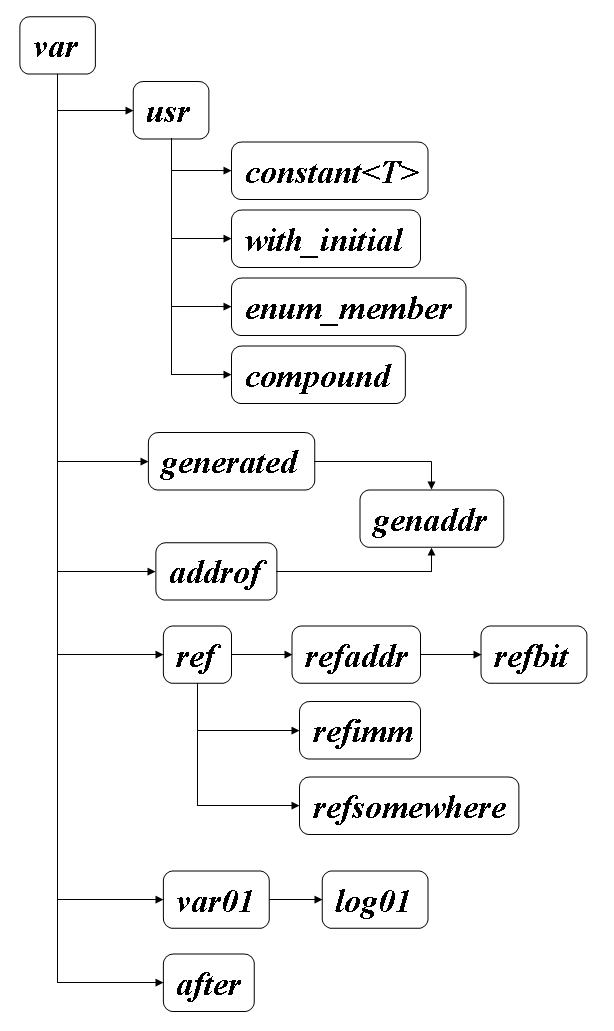
\includegraphics[width=1.0\linewidth,height=1.626\linewidth]{var.png}
\end{htmlonly} 
\begin{latexonly}
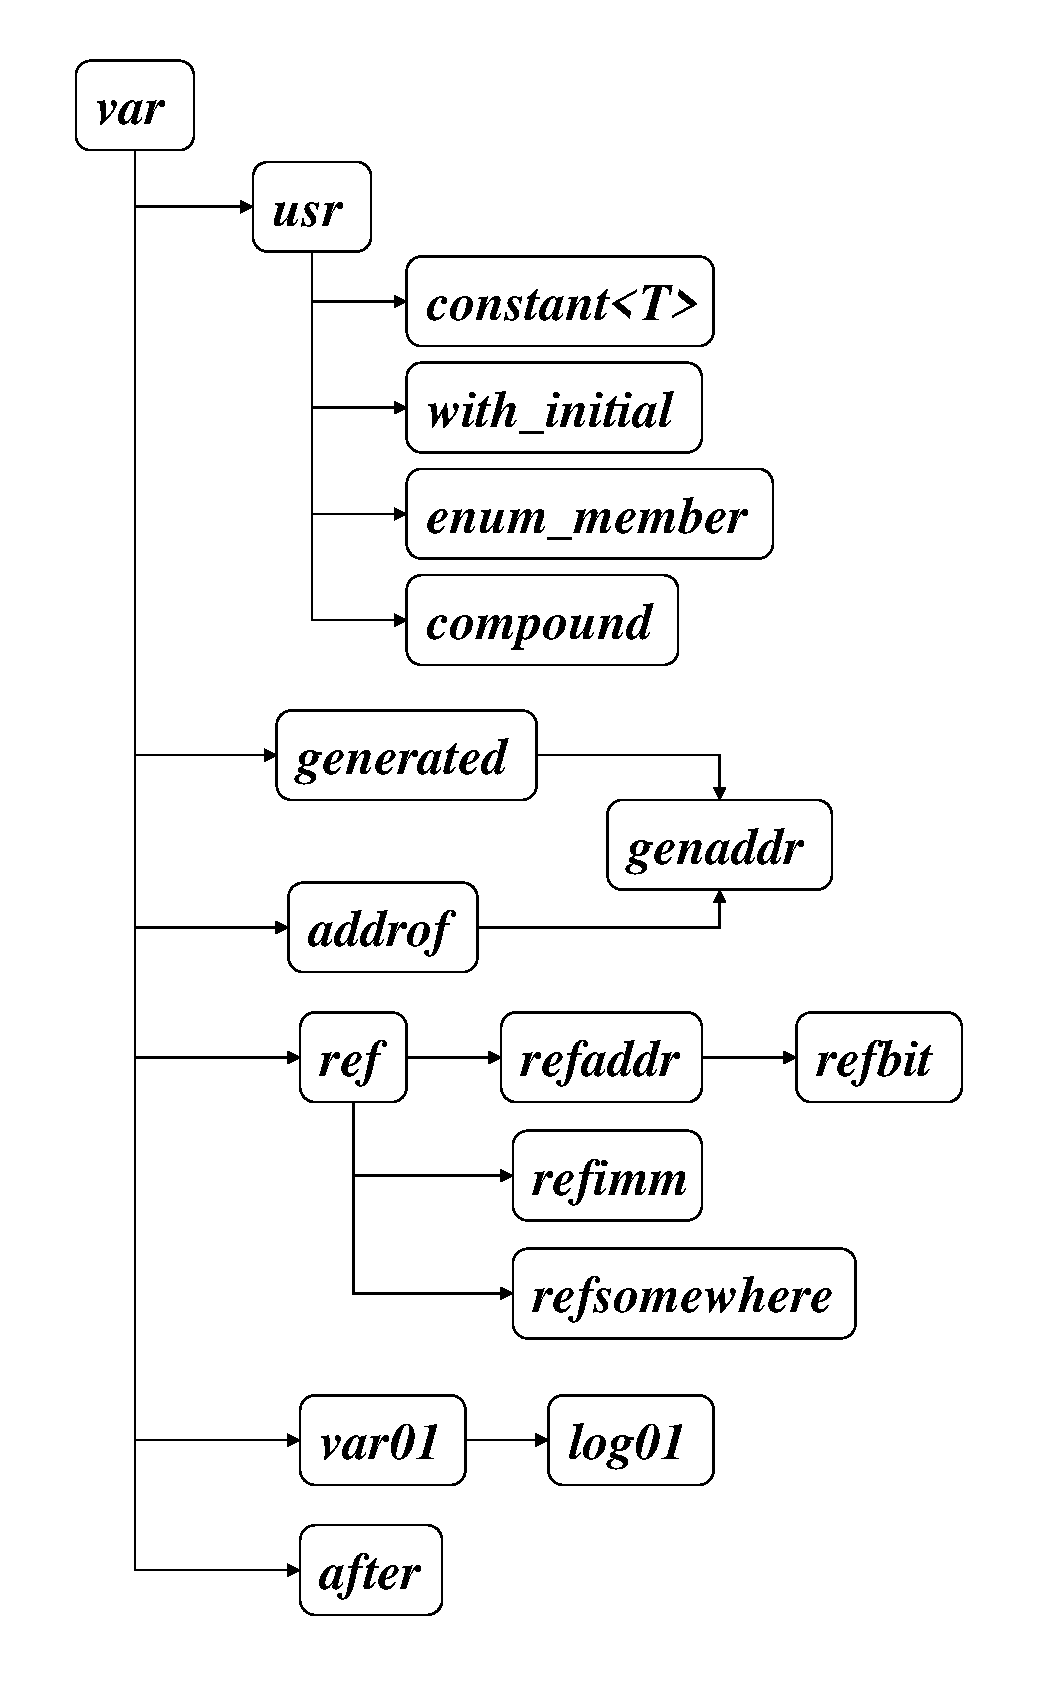
\includegraphics[width=1.0\linewidth,height=1.626\linewidth]{var.eps}
%%\includegraphics[width=1.8\linewidth,height=2.35\linewidth]{var2.eps}
\end{latexonly}
\caption{{\tt{var}} and derived class}
\label{expr_e013}
\end{center}
\end{figure}

As described in \ref{lex_yacc_e003}, 
while bottom-up parsing, frontend just makes instances
derived from {\tt{expr}}, where
\begin{verbatim}
class expr {
public:
  virtual var* eval() = 0;  // Evaluate expression
  virtual ~expr(){}
};
\end{verbatim}
And frontend calls virtual function {\tt{expr::eval}} if necessary.

\section{\tt{primary-expression}}
\label{expr_e015}
\index{primary-expression@\tt{primary-expression}}
{\tt{primary-expression}} is one of identifier, integer constant,
character constant, floating constant, string literal, enumeration
constant and parenthized expression. If {\tt{primary-expression}} is 
one of these except for parenthized expression, the attribute of token
is pointer to {\tt{var}}. And if {\tt{primary-expression}} is 
parenthized expression, we can get the pointer to {\tt{expr}}.
{\tt{primary-expression}} can be represented like below.
\begin{verbatim}
class prim_expr : public expr {
  var* m_var;
  expr* m_expr;
public:
  prim_expr(var* v) : m_var(v), m_expr(0) {}
  prim_expr(expr* e) : m_var(0), m_expr(e) {}
  var* eval();
};
\end{verbatim}

In C language, if the type of sub-expression is array or function,
pointer generation rule is applied. About pointer generation,
See bibliography
\cite{KR} ``A7.1 pointer generation'' or
bibliography \cite{ISO} ``6.2.2.1 Lvalues and function designators'', please.
{\tt{prim\_expr::eval}} will be like below.
\begin{verbatim}
var* prim_expr::eval()
{
  if ( m_expr )  // Parenthized expression
    return m_expr->eval();

  if m_var is a member of enumeration, return the correspond integer value.

  typedef const pointer_type PT;
  const type* T = m_var->m_type;
  if ( const PT* pt = T->pointer_gen() ) {
    // Array or function case
    return new genaddr(m_var,...);
  }
  else
    return m_var;
}
\end{verbatim}
If pointer generation rule is applied, we'll represent the result of
the evaluated expression as {\tt{genaddr}} in figure \ref{expr_e013}.
Considering that {\tt{genaddr}} is used in the situation
where pointer generation rule isn't applied or {\tt{genaddr}} is used
as static variable initial value,
3 address code {\tt{x := \&y}} is generated only if necessary.

\section{\tt{postfix-expression}}
\index{postfix-expression@\tt{postfix-expression}}

\subsection{Subscripting operator}
\label{expr_e017}
\index{subscripting operator@subscripting operator}

Consider below program.
\begin{verbatim}
void f(double* p, int i, int j){ p[j] = p[i]; }
\end{verbatim}
Assume that {\tt{sizeof(double) = 8}},
frontend will generate 3 address codes like below.
\begin{verbatim}
f:
  t0 := i * 8             # int t0
  t1 := p + t0            # double* t1
  t2 := j * 8             # int t2
  t3 := p + t2            # double* t3
  t4 := *t1               # double t4
  *t3 := t4
\end{verbatim}
For right hand subscripting operator, 
consequentially frontend generated 3 address code {\tt{x := *y }}.
On the other hand, for left hand subscripting operator,
frontend generated 3 address code {\tt{*y := z }}.
That is, generated 3 address code depends on usage as lvalue or rvalue.

Consider another program.
\begin{verbatim}
double a[10];
void g(int i){ a[5] = a[i]; }
\end{verbatim}
Frontend will generate 3 address codes like below.
\begin{verbatim}
g:
     t0 := 8 * i          # int t0
     t1 := a[t0]          # double t1
  a[40] := t1
\end{verbatim}
For right hand subscripting operator, 
frontend generated 3 address code {\tt{x := y[z] }}.
On the other hand, for left hand subscripting operator,
frontend generated 3 address code {\tt{x[y] := z}}.
Samely, generated 3 address code depends on usage as lvalue or rvalue.

These two examples shows that we should change the way of evaluating
subscripting operator according to subscripting operator opearnd
in figure \ref{expr_e013}. So we'll implement this as virtual function
like below.
\begin{verbatim}
struct var {
  ...
  virtual var* subscripting(var* index);
};

struct genaddr : generated, addrof {
  ...
  var* subscripting(var* index);  // Override virtual function
};
\end{verbatim}
where, {\tt{genaddr}} is the result of pointer generation described in
\ref{expr_e015}. {\tt{genaddr::subscripting}} will be like below.
\begin{verbatim}
// For `m_ref', pointer generation rule was applied, and then
// subscripting operator is used with operand `index'
var* genaddr::subscripting(var* index)
{
  index = index->rvalue();
  if ( !index->m_type->integer() ) {
    // The type of index is not integer. Error. 
  }
  typedef const array_type AT;
  AT* at = dynamic_cast<AT*>(m_ref->m_type);
  if ( !at ) {
    // Subscripting operator is applied to function type. Error.
  }
  const type* T = at->element_type();
  var* size = integer::create(T->size());
  var* offset = expr::binary('*', size, index);
  return offref(T,offset);  // Call virtual function
}
\end{verbatim}
We'll discuss about virtual function `{\tt{offref}}' later,
but here, for easy, we just say that virtual function `{\tt{offref}}'
returns `{\tt{ref}}' or derived class from `{\tt{ref}}' in
figure \ref{expr_e013}.
The reason why we use class derived from `{\tt{ref}}' is
that generated code is depend on usange as lvalue or rvalue.
In the first line of {\tt{genaddr::subscripting}}, we'll call virtual function
`{\tt{var::rvalue}}' for using the result of some expression as rvalue.

Samely, {\tt{var::subscripting}} will be like below.
\begin{verbatim}
var* var::subscripting(var* index)
{
  var* array = rvalue();
  index = index->rvalue();
  if ( !index->m_type->integer() )
    swap(array,index);
  if ( !index->m_type->integer() ) {
    // The type of index is not integer. Error.
  }
  typedef const pointer_type PT;
  PT* pt = dynamic_cast<PT*>(array->m_type);
  if ( !pt ) {
    // array->m_type is not pointer. Error.
  }
  const type* T = pt->reference_type();
  var* size = integer::create(T->size());
  var* offset = size->mul(index);
  return array->offref(T,offset);  // Call virtual function
}
\end{verbatim}
If `{\tt{offset}}' is constant, the result of this operator must not be
{\tt{var}}. For example,
\begin{verbatim}
/* Global scope */
int a[5][6];
int* p = &a[3][4];  /* Initial value of `p' is
                       address of `a' + sizeof(int) * 22 */

int* q = &((int*)0x5678)[9];  /* Initial value of `q' is
                                 0x5678 + sizeof(int) * 9 */
\end{verbatim}
Now, we'll define the virtual function `{\tt{offref}}', and
override it if necessary like below.
\begin{verbatim}
struct var {
  ...
  virtual var* offref(const type* T, int offset)
  {
    // General case.
    var* ret = new ref(T);
    ...  // Generate 3 address codes for calculating address.
    return ret;
  }
};

struct genaddr : generated, addrof {
  ...
  var* offref(const type* T, var* offset)  // Override virtual function
  {
    if ( offset->isconstant() ) {
      // In this case, return `refaddr'.
      int off = m_offset + offset->int_value();
      return new refaddr(pointer_type::create(T),
                         m_ref,off);
    }

    // In this case, return `refsomewhere'
    offset = offset->add(integer::create(m_offset));
    return new refsomewhere(pointer_type::create(T),
                            m_ref,offset);
  }
};

// Special version of constat<T>
template<> struct constant<void*> : usr {  // constant pointer
  void* m_value;
  ...
  var* offref(const type* T, int offset)  // Override virtual function
  {
    if ( offset->isconstant() ) {
      int off = offset->int_value();
      char* p = reinterpret_cast<char*>(m_value);
      return new refimm(pointer_type::create(T),p+off);
    }
    return var::offref(T,offset);
  }
};
\end{verbatim}
Actually, it is necessary to override virtual function `{\tt{offref}}'
in class `{\tt{addrof}}', `{\tt{refaddr}}' and `{\tt{refsomewhere}}'.
But for easy, omitted.
%% struct refaddr : ref {
%%   addrof* m_addrof;
%%   int m_offset;
%%   ...
%%   var* offref(const type* T, int offset)  // Override virtual function
%%   {
%%      // The offset was `m_addrof.m_offset'. Now add `offset',
%%      // and reference the same object.
%%      return new refaddr(pointer_type::create(T),
%%                         m_addrof.m_ref,m_addrof.m_offset+offset);
%%   }
%% };

\subsection{Function call operator}
\label{expr_e006}
\index{function call operator@function call operator}

For function type, pointer generation rule is applied
samely with array type. Because we want to generate 3 address code
{\tt{x := \&y}} only if necessary,
we'll implement this as virtual function, samely with subscripting
operator like below.
\begin{verbatim}
struct var {
  ...
  virtual var* call(const vector<var*>& arg);
};

struct genaddr : generated, addrof {
  ...
  var* call(const vector<var*>& arg);  // Override virtual function
};
\end{verbatim}
Actually, frontend must generate 3 address codes
for calling {\tt{inline}} function, but here for easy,
{\tt{genaddr::call}} will be like below.  
\begin{verbatim}
// For `m_ref', pointer generation rule was applied, and then
// function call operator is used with operand `arg'
var* genaddr::call(const vector<var*>& arg)
{
  typedef const func_type FT;
  FT* ft = dynamic_cast<FT*>(m_ref->m_type);
  if ( !ft ) {
    // Not function. Error.
  }
  return call_impl::common(ft,m_ref,arg);
}
\end{verbatim}
Considering that function call operator can be used for not
declared function in C language, 
{\tt{var::call}} will be like below.
\begin{verbatim}
var* var::call(const vector<var*>& arg)
{
  var* func = rvalue();
  const type* T = func->m_type;
  if ( func is not in symbol table ) {
    // Insert func into symbol table, here.
    usr* u = static_cast<usr*>(func);
    string name = u->m_name;
    u->m_type = T = func_type::create(int_type::create(),...);
    scope::current->m_usrs[name] = u;
  }
  else {
    // function call via pointer to function
    typedef const pointer_type PT;
    PT* pt = dynamic_cast<PT*>(T);
    if ( !pt ) {
      // Not pointer. Error.
    }
    T = pt->reference_type();
  }
  typedef const func_type FT;
  FT* ft = dynamic_cast<FT*>(T);
  if ( !ft ) {
    // Not function. Error.
  }
  return call_impl::common(ft,func,arg);
}
\end{verbatim}

It's neccesary to compare
the number of called function parameters and
the number of arguments while evaluating function call operator.
Especially in C language, 
A function may be called with a variable number of arguments,
whose function type expression is represented with {\tt{ellipsis\_type}},
as described in \ref{type_e004}. We'll implement like below.
\begin{verbatim}
// Get range of number of arguments from parameter
pair<int,int>
call_impl::num_of_range(const vector<const type*>& param)
{
  const type* T = param.back();
  typedef const ellipsis_type ELLIPSIS;
  if ( ELLIPSIS* ellipsis = dynamic_cast<ELLIPSIS*>(T) )
    return make_pair(param.size()-1,numeric_limits<int>::max());

  return T->compatible(void_type::create()) ? make_pair(0,0)
    : make_pair(param.size(),param.size());
}
\end{verbatim}

\begin{verbatim}
var* call_impl::common(const func_type* ft, var* func,
                       const vector<var*>& arg)
{
  int n = arg.size();
  const vector<const type*>& param = ft->param();
  pair<int,int> m = num_of_range(param);
  if ( n < m.first ) {
    // Too few arguments. Error.
  }
  else if ( m.second < m ) {
    // Too many arguments. Error.
  } 
  ...
}
\end{verbatim}

And more, it's necessary to judge that an argument
can be converted to the correspond parameter type.
This conversion is valid if and only if assignment is valid.
\begin{verbatim}
var* call_impl::convert(var* arg, const type* T)
{
  arg = arg->rvalue();
  T = assign_impl::valid(T,arg);
  if ( !T ) {
    // Invalid assignment. Error.
  }
  return arg->cast(T);
}

tac* call_impl::new_param(var* y){ return new param(y); }

var* call_impl::common(const func_type* ft, var* func,
                       const vector<var*>& arg)
{
  ...
  vector<var*> conved;
  transform(arg.begin(),arg.end(),param.begin(),back_inserter(conved),
            convert);
  transform(conved.begin(),conved.end(),back_inserter(code),new_param);
  ...
}
\end{verbatim}

And finally, frontend shall generate 3 address code {\tt{call}}.
Note that function declaration returing function and
function declaration returning array are error,
but function declaration returning incomplete tagged type
is not error. And also that function call is error, which 
returns incomplete tagged type. Frontend must check this like below.
\begin{verbatim}
void f(void)
{
  struct S g();  /* Function returning incomplete tagged type. OK.  */
  g();  /* Error. */
  struct S { int a; };
  g();  /* OK. */
}
\end{verbatim}
The correspond part of {\tt{call\_impl::common}} will be like below.
\begin{verbatim}
var* call_impl::common(const func_type* ft, var* func,
                       const vector<var*>& arg)
{
  ...
  const type* T = ft->return_type();
  var* ret = new var(T);
  if ( T->compatible(void_type::create()) ) {
    code.push_back(new call3ac(0,func));
    return ret;
  }
  T = T->complete_type();
  if ( !T->size() ) {
    // Call function returning incomplete tagged type. Error.
  }
  scope::current->m_vars.push_back(ret);  // Insert the result
                                          // into symbol table
  code.push_back(new call3ac(ret,func));
  return ret;
}
\end{verbatim}

\subsection{Member reference operator}
\label{expr_e024}
\index{member reference operator@member reference operator}

Let frontend to make node like below for member reference operator,
while bottom-up parsing.
\begin{verbatim}
class member : public expr {
  var* m_var;           // left operand
  std::string m_name;   // right operand
  bool m_dot;           // true if . operator, false if -> operator
public:
  ...
  var* eval();
};
\end{verbatim}
Note that {\tt{(*$\alpha$).$\beta$}} shall be evaluated
samely with {\tt{$\alpha$->$\beta$}}.
Consider below example.
\begin{verbatim}
  struct T { int c; int b; } *a;
  ...
  (*a).b = 1;
\end{verbatim}
Assume that {\tt{sizeof(int) = 4}}. If frontend generates below
3 address codes
\begin{verbatim}
  t0 := *a      # struct T t0
  t1 := &t0     # int* t1
  t1 := t1 + 4
 *t1 := 1
\end{verbatim}
it's not correct. In these codes, {\em copied} object offset 4
is written, which is copied from the area pointed by {\tt{a}}.
Correct 3 address codes become like below.
\begin{verbatim}
  t1 := a + 4   # int* t1
 *t1 := 1
\end{verbatim}
Therefore, it's not correct to call virtual function {\tt{rvalue}}
for member {\tt{m\_var}} in {\tt{member::eval}}.
{\tt{member::eval}} will be like below easily.
\begin{verbatim}
var* member::eval()
{
  // Not evaluate for m_var. Just get the result type.
  const type* T = m_var->result_type();  // Call virtual function.

  T = T->unqualified();
  typedef const pointer_type PT;
  if ( !dot ) {
    PT* pt = dynamic_cast<PT*>(T);
    if ( !pt ) {
      // Applied -> operator for not pointer. Error.
    }
    T = pt->referenced_type();
    T = T->unqualified();
  }
  T = T->complete_type();
  typedef const record_type REC;
  REC* rec = dynamic_cast<REC*>(T);
  if ( !rec ) {
    // Either structure nor union. Error.
  }
  pair<int, usr*> off = rec->offset(m_name);
  int offset = off.first;
  if ( offset < 0 ) {
    // Not member. Error.
  }
  usr* member = off.second;
  T = member->m_type;
  if ( member->m_flag & usr::BIT_FIELD ) {
    // Reference bit-field. Speciall case.
    return new refbit(...);
  }
  var* off = integer::create(offset);
  return m_var->offref(T,off);  // Call virtual function.
}
\end{verbatim}

\subsubsection{Lvalue}
\label{expr_e023}
Now here, we'll mention about lvalue digressing from
evaluating member reference operator.
In C language, below expressions may have lvalue.
\begin{enumerate}
\item identifier. {\tt{a = 1;}}
\item string-literal ( not valid if it appears in left hand of
assignment operator, but it can be operand of unary {\tt{\&}} operator).
{\tt{\&"foo";}}
\item subscripting operator. {\tt{a[b] = c;}}
\item {\tt{.}} operator. {\tt{a.b = c;}}
\item {\tt{->}} operator. {\tt{a->b = c;}}
\item {\tt{compound-literal}} (valid even if it appears in left hand of
assignment operator). {\tt{\&(struct S)\{1,2\};}}
\item unary {\tt{*}} operator. {\tt{*a = b;}}
\item parenthized above expression. {\tt{(a) = b;}}
\end{enumerate}
Here, please note that {\tt{->}} operator always has lvalue,
but on the other hand {\tt{.}} operator doesn't always have lvaue.
For example,
\begin{verbatim}
  struct S f();
  f().a = 1;  /* The result of call operator doesn't have lvalue.
                 Error. */
\end{verbatim}
Expression {\tt{$\alpha$.$\beta$}} has lvalue if and only if
$\alpha$ has lvalue.
Now, we should not consider lvalue as attribute of expression.
We should consider lvalue as attribute of the result of evaluating
expression. i.e. make it virtual function of {\tt{var}} like below.
\begin{verbatim}
struct var {
  ...
  virtual bool lvalue(){ return false; }
};
\end{verbatim}

The result of evaluating {\tt{.}} operator will be
{\tt{refaddr}} in figure \ref{expr_e013}, so, return {\tt{false}}
in {\tt{refaddr::lvalue}} if left operand doesn't have lvalue.
Or you can change the result of evaluating {\tt{.}} operator
to {\tt{var}}. This can catch the above example error.

\subsection{Postfix {\tt{++}}, {\tt{--}} operator}
\label{expr_e007}
\index{++@{\tt{++}}}
\index{--@{\tt{--}}}

The result of evaluating post {\tt{++}}, {\tt{--}} operator 
becomes the medium variable (i.e. {\tt{var}}) and then
increment or decrement 3 address codes shall be generated.
Very simple example is
\begin{verbatim}
  int a; ...; a++;

  t0 := a      # int t0 : the result of evaluating a++ 
  a := a + 1
\end{verbatim}

Consider if post {\tt{++}},  {\tt{--}} is applied to the result which was
applied to the pointer generation rule.
\begin{verbatim}
  int a[10];
  void f(void);
  ...
  a++;  /* Error. ++ for array type. */
  f--;  /* Error. -- for function type. */
\end{verbatim}
From this example, we can immediately make it error
if {\tt{++}} or {\tt{--}} is applied to the result which was
applied to the pointer generation rule, i.e, {\tt{generated}} 
in figure \ref{expr_e013}.
\begin{verbatim}
struct var {
  ...
  // Evaluate the result of ++, --
  virtual var* ppmm(bool plus, bool post)
  {
    // Not lvalue. Error.
  }
};

struct usr : var {
  ...
  var* ppmm(bool plus, bool post)  // Override virtual function
  {
    // If this is variable in program text and modifiable,
    // generate 3 address code.
  }
};

struct generated : var {
  var* ppmm(bool plus, bool post)  // Override virtual function
  {
    // Immediately error.
  }
};
\end{verbatim}

Consider also about {\tt{ref}} in figure \ref{expr_e013}.
{\tt{ref}}'s 3 address codes are depend on usange as lvalue or rvalue.
\begin{verbatim}
  char *a; ...; (*a)++;
\end{verbatim}
For this program, 3 address codes become like below.
\begin{verbatim}
                  # The result of *a becomes `ref'
  t0 := *a        # char t0
                  # Because post ++ is applied for (*a),
                  # evaluate *a. t0 is the result of (*a)++.
  t1 := (int)t0   # int t1
                  # Type of t0 is char, so, prmote to int.
  t1 := t1 + 1
  t2 := (char)t1  # Convert t1 to original type
  *a := t2 
\end{verbatim}

\subsection{{\tt{compound-literal}}}

{\tt{compound-literal}} is defined in ISO C.
See bibliography \cite{ISO}, please.
Evaluating {\tt{compound-literal}} is replaced with
evaluating initializer as described in section \ref{decl_e005}.
\begin{verbatim}
struct S { int a; int b; };

struct S a = (struct S){1, 2};  /* Global scope. Just permitted
                                   initializer constant in 
                                   initializer-list. Equivalent to
                                   struct S a = { 1, 2 }; */

struct S* b = &(struct S){3, 4};  /* Make the medium variable
                                     in global scope, whose type
                                     is struct S. And whose address
                                     becomes initial value of `b'.
                                     Initial value of the medium
                                     variable are 3, 4.
                                  */
void f(int x, int y)
{
  void g(struct S*);
  g(&(struct S){x, y});  /* compound-literal has lvalue
                            like string-literal. So, it can be
                            operand of unary & operator. */

  int *p = (int []){x, y};  /* type-name is incomplete array type,
                               but initializer-list makes it int [2].
                               Tye type of right hand becomes int*
                               after pointer generation rule.
                             */

  (int){1} = 2;  /* The medium variable whose type is int
                    is initialzed with 1, and then it is
                    applied assignment operator. The medium
                    variable becomes 2. */
}
\end{verbatim}

\section{\tt{unary-expression}}
\label{expr_e008}
\index{unary-expression@\tt{unary-expression}}

\subsection{Prefix {\tt{++}}, {\tt{--}} operator}
\index{++@{\tt{++}}}
\index{--@{\tt{--}}}

We described about postfix {\tt{++}}, {\tt{--}} operator in
\ref{expr_e007}.
The result of prefix {\tt{++}}, {\tt{--}} operator is
the value after incrementing or decrementing.

\subsection{Unary {\tt{\&}} operator}
\label{expr_e019}

This operator requires operand which has lvalue.
We have represented the result of evaluating expression
as the class in figure \ref{expr_e013}.
So, for unary {\tt{\&}} operator,
we'll define virtual function and override it in each class
if necessary.
\begin{verbatim}
struct var {
  ...
  virtual var* address(){ /* Not lvalue. Error. */ }
};

struct usr : var {
  flag_t m_flag;  // storage class etc
  ...
  var* address();  // Override virtual function
};
\end{verbatim}
Address of the variable which appears in program text
is evaluated by {\tt{usr::address}}.
\begin{verbatim}
var* usr::address()
{
  if ( !lvalue() )
    // Not lvalue. Error.

  if ( m_flag & REGISTER )
    // Storage class `register' is specified. Error.

  typedef const poitner_type PT;
  PT pt = pointer_type::create(m_type);
  block* b = dynamic_cast<block*>(scope::current);
  if ( b && constant-expression is being evaluating ) {
    // In this case, generate 3 address code
    var* ret = new var(pt);
    b->m_vars.push_back(ret);
    code.push_back(new addr3ac(ret,this));
    return ret;
  }
  else
    return new addrof(pt,this,...);
}
\end{verbatim}
Unary {\tt{\&}} operator is the exception case of pointer generation
rule. So, we'll define {\tt{genaddr::address}}.
\begin{verbatim}
struct genaddr : generated, addrof {
  ...
  var* address();  // Override virtual function
};

var* genaddr::address()
{
  // Decide to generate 3 address code or
  // to return just `addrof' samely with `usr::address'
}
\end{verbatim}

\begin{QandA}
Does it matter if we don't override virtual function `{\tt{address}}' in
class {\tt{generated}}?

Answer : It depens on implementation. It's fact that
unary {\tt{\&}} operator is the exception case of pointer generation
 rule.
But in an implementation, {\tt{generated}} is used in the very limited
situation for representing the result of evaluating expression.
In such an implementation, virtual function `{\tt{address}}' will not
be called for {\tt{generated}}, so, it shouldn't be overridden.
Or, override it like below.
\begin{verbatim}
var* generated::address(){ assert(0); /* Internal error. */ } 
\end{verbatim}
On the other hand, we want to represent the result of evaluating expression
as {\tt{addrof}} in {\tt{genaddr::address}}.
 But it can't be in {\tt{generated}}.
\end{QandA}
It is neccesary that virtual function {\tt{address}} is overridden
for {\tt{ref}} or class derived from it in figure \ref{expr_e013}.
\begin{verbatim}
var* ref::address() // Override virtual function
{
  // In this case, always generate 3 address code
  var* ret = new var(m_type);
  code.push_back(new assign3ac(ret,this));
  return ret;
}

var* refaddr::address() // Override virtual function
{
  // Decide to generate 3 address code or
  // to return just `addrof' samely with `usr::address'
  // and `genaddr::address'
}

var* refbit::address()  // Override virtual function
{
  // Apply unary & operator for bit field. Error.
}

var* refimm::address()  // Override virtual function
{
  return new constant<void*>(...);
}

var* refsomewhere::address()  // Override virtual function
{
  // Generate 3 address codes for calculating address.
}
\end{verbatim}

\subsection{Unary {\tt{*}} operator}
\label{expr_e009}

3 address code for unary {\tt{*}} operator depends on
using as lvalue or rvalue. So, the result of evaluating unary
{\tt{*}} operator must be represented as
{\tt{ref}} or {\tt{refaddr}} in figure \ref{expr_e013}.
This operator also is evaluated with virtual function.
\begin{verbatim}
struct var {
  ...
  virtual var* indirection();  // evaluate unary * operator
};

var* var::indirection()
{
  var* y = rvalue();
  const type* T = y->m_type;
  T = T->unqualified();
  typedef const pointer_type PT;
  PT* pt = dynamic_cast<PT*>(T);
  if ( !pt ) {
    // Not pointer. Error.
  }
  ref* x = new ref(pt);
  code.push_back(new assign3ac(x,y));
  return x;
}
\end{verbatim}
We should change the way of evaluating unary {\tt{*}} operator
for {\tt{addrof}}, {\tt{genaddr}} and {\tt{constant<void*>}}
in figure \ref{expr_e013}
For example,
\begin{verbatim}
/* Global scope */
int a; int* p = &*&a;  /* Initial value of `p' is address of `a' */

void f(void); void g(void){ (****************f)(); }  /* OK */

int* q = &*(int*)0x1234;  /* Initial value of `q' is 0x1234 */
\end{verbatim}
So, override the virtual function and do work specially
in {\tt{addrof::indirection}}, {\tt{genaddr::indirection}} and
{tt{constant<void*>::indirection}}.
Now, we can generate single 3 address code `{\tt{call f}}' for `{\tt{g}}'.

\subsection{Unary {\tt{+}} operator}

The result of unary {\tt{+}} operator doesn't have lvalue.
We must represent the result of evaluating unary {\tt{+}} operator
as something none-lvalue.
\begin{verbatim}
struct var {
  ...
  var* plus(){ ... return this; }  // Not virtual function. Incorrect.
};
\end{verbatim}
And we must take care of the situation where unary {\tt{+}} operator
is used for arithmetic constant and it is specified to static 
variable initializer. Similary so far, we'll define the virtual function
and override it if necessary.
\begin{verbatim}
struct var {
  ...
  virtual var* plus();  // Virtual function
};

template<class T> struct constant : usr {
  ...
  var* plus();  // Override virtual function
};
\end{verbatim}
We always generate 3 address code in {\tt{var::plus}},
but it will be erased in optimization phase.
{\tt{var::plus}} becomes like below.
\begin{verbatim}
var* c_compiler::var::plus()
{
  var* expr = rvalue();
  const type* T = expr->m_type;
  if ( !T->arithmetic() ) {
    // Not arithmetic. Error.
  }
  T = T->promotion();
  expr = expr->cast(T);
  var* ret = new var(T);
  if ( block* b = dynamic_cast<block*>(scope::current) )
    b->m_vars.push_back(ret);
  code.push_back(new assign3ac(ret,expr));
  return ret;
}
\end{verbatim}
On the other hand, constant doesn't have lvalue, so,
{\tt{constant<T>::plus}} becomes like below.
\begin{verbatim}
template<class T> var* constant<T>::plus(){ ... return promotion(); }
\end{verbatim}

\subsection{Unary {\tt{-}} operator}
The point is the same with uanry {\tt{+}} operator.
For unary {\tt{-}} operator, frontend must do runtime-evaluation
in {\tt{constant<T>::minus}}
\begin{verbatim}
struct var {
  ...
  virtual var* minus()  // Virtual function
  {
    // generate 3 address code x := -y
  }
};

template<class T> struct constant : usr {
  ...
  var* minus()  // Override virtual function. do runtime-evaluation.
  {
    // Apply unary - operator for containg constant value,
    // create struct constant for it, and return it.
  }
};
\end{verbatim}

\subsection{{\tt{\~{}}} operator}

Samely with unary {\tt{+}} and {\tt{-}} operator.
The operand of this operator must be integer type.

\subsection{{\tt{!}} operator}
\label{expr_e016}
{\tt{!}} operator is defined for scalar operand. Frontend generates
corresponding zero for the operand and compares with it. If not equal,
the result of this operator becomes 0, otherwise 1. If 3 addres codes
are generated for this operator, some of them become conditional or 
unconditional jump. So, {\tt{!}} operator is different with other unary
operators at this point. But if {\tt{!}} operator is applied to
{\tt{constant}}, frontend must do runtime-evaluation. Similary so far,
\begin{verbatim}
struct var {
  ...
  virtual var* not();  // Virtual function
};

template<class T> struct constant : usr {
  ...
  var* not()  // Override virtual function
  {
    // return 0 or 1
  }
};
\end{verbatim}
For example, 3 address codes becomes like below
of evaluating {\tt{!*p}} for {\tt{char* p}}.
\begin{verbatim}
  t0 := *p                 # char t0
  t1 := (int)t0            # int t1
  if t1 != 0 goto label
  t2 := 1                  # int t2
  goto label2
label:
  t2 := 0
label2:
\end{verbatim}
In this case, {\tt{t2}} is the result of evaluating {\tt{!}} operator.
Please note that the result of this operator is used in
{\tt{if}} statement expression or conditional part of loop statement.
We want to generate fewer 3 address codes in this situation
by replacing 3 address codes for {\tt{t2}}.
For this, we don't represent the result of this operator as {\tt{var}},
represent it as {\tt{var01}} in figure \ref{expr_e013}. That is,
\begin{verbatim}
struct var {
  ...
  virtual void if_expr(); // Virtual function for generating
                          // if statement 3 address code
};

struct var01 : var {
               // For t2 in above example,
  int m_one;   // the position in t2 := 1
  int m_zero;  // the position in t2 := 0
  ...
  void if_expr();  // Override virtual function
                   // generate fewer 3 address code
};
\end{verbatim}
In the next chapter, we'll discuss about generating 3 address codes
for statements. Now {\tt{var::not}} becomes like below.
\begin{verbatim}
var* var::not()
{
  var* expr = rvalue();
  const type* T = expr->m_type;
  if ( !T->scalar() ) {
    // Not scalar. Error.
  }
  expr = expr->promotion();
  usr* zero = integer::create(0);
  usr* one = integer::create(1);
  var01* ret = new var01(int_type::create());
  if ( block* b = dynamic_cast<block*>(scope::current) )
    b->m_vars.push_back(ret);
  var* tmp = zero->cast(expr->m_type);
  goto3ac* goto1 = new goto3ac(goto3ac::NE,expr,tmp);
  code.push_back(goto1);
  ret->m_one = code.size();
  code.push_back(new assign3ac(ret,one));
  goto3ac* goto2 = new goto3ac;
  code.push_back(goto2);
  to3ac* to1 = new to3ac;
  to1->m_goto.push_back(goto1);
  code.push_back(to1);
  goto1->m_to = to1;
  ret->m_zero = code.size();
  code.push_back(new assign3ac(ret,zero));
  to3ac* to2 = new to3ac;
  code.push_back(to2);
  to2->m_goto.push_back(goto2);
  goto2->m_to = to2;
  return ret;
}
\end{verbatim}

\subsection{{\tt{sizeof}} operator}
\index{sizeof@\tt{sizeof}}

It's incorrect that frontend generates 3 address codes
for expression which is applied {\tt{sizeof}} operator.
For not doing so, frontend must remember the number of 3 address codes
before evaluating expression applied {\tt{sizeof}} operator,
and after generating 3 address code for the expression,
frontend must erase new 3 address codes.
\begin{verbatim}
struct sizeof_expr : expr {
  const type* m_type;
  expr* m_expr;
  sizeof_expr(const type* T) : m_type(T), m_expr(0) {}
  sizeof_expr(expr* E) : m_type(0), m_expr(E) {}
  virtual var* eval()
  {
    if ( m_type ) {
      int n = m_type->size();
      if ( !n ) {
        // Sizeof operator is applied for incomplete type,
        // function type or void. Error.
      }
      return integer::create(n);
    }

    int m = code.size();  // The number of 3 address codes
                          // before evaluating `m_expr'
    var* ret = m_expr->eval();
    ret = ret->size();  // Call virtual function
    code.resize(m);  // At this point, erase new 3 address codes.
    return ret;
  }
};
\end{verbatim}
Similary so far, we'll define virtual function for {\tt{sizeof}} operator.
\begin{verbatim}
struct var {
  virtual var* size();  // Virtual function
};

var* var::size()
{
  var* y = rvalue();
  int n = y->m_type->size();
  if ( !n ) {
    // Sizeof operator is applied for incomplete type
    // or void. Error.
  }
  return integer::creat(n);
}
\end{verbatim}
If the result of evaluating expression is 
made by the pointer generation rule and it is applied
{\tt{sizeof}} operator, it is the exception case
of pointer generation rule.
\begin{verbatim}
struct generated : virtual var {
  const type* m_org;  // Type before pointer generation rule applied
  ...
  var* size()  // Override virtual function
  {
    int n = m_org->size();
    if ( !n ) {
      // Sizeof operator is applied for function
      // or incomplete array type. Error.
    }
    return integer::create(n);
  }
};
\end{verbatim}
Frontend catches the error if {\tt{sizeof }} operator is applied
for bit field.
\begin{verbatim}
struct refbit : refaddr {
  ...
  var* size() // Override virtual function
  {
    // Sizeof operator is applied for bit field.
    // Error.
  }
};
\end{verbatim}

\section{\tt{cast-expression}}
\index{cast-expression@\tt{cast-expression}}

The type of {\tt{cast-expression}} can be scalar type
and {\tt{void}}. But the conversion from pointer type to floating type
or the opposite conversion is not permitted.
\begin{verbatim}
class cast_expr : expr {
  const type* m_type;
  expr* m_expr;
  cast_expr(const type* T, expr* E) : m_type(T), m_expr(E) {}
  var* eval()  // Override virtual function
  {
    var* y = m_expr->eval();
    y = y->rvalue();
    if ( m_type->compatible(void_type::create()) ){
      var* ret = new var(void_type::create());
      return ret;
    }
    if ( !m_type->scalar() ){
      // Not scalar. Error.
    }
    m_type = cast_impl::valid(m_type,y);
    if ( !m_type ){
      // Conversion between pointer type and floating type. Error.
    }
    return expr->cast(m_type); // Call virtual function.
  }
};
\end{verbatim}
Actually, we used virtual function `{\tt{var::cast}}', for example,
in function call operator where an argument is converted to
correspond parameter type. Similary so far,
we'll define virtual function and override it if necessary.
\begin{verbatim}
struct var {
  ...
  virtual var* cast(const type*);  // Virtual function. General work.
};

template<class T> struct constant : usr {
  ...
  var* cast(const type*);  // Override virtual function.
                           // Frontend must do runtime-evaluation.
};

struct addrof : virtual var {
  ...
  var* cast(const type*);  // Override virtual function.
                           // Return `addrof'.
};
\end{verbatim}

\section{\tt{multiplicative-expression}}
\label{expr_e011}
\index{multiplicative-expression@\tt{multiplicative-expression}}

Binary {\tt{*}}, {\tt{/}} operator is defined for arithmetic type.
And {\tt{\%}} operator is defined for integer type.
Before operation, usual arithmetic conversion is performed
described in bibliography \cite{ISO} 6.2.1.7.
For easy, we'll think about binary {\tt{*}} operator in this section.

Similary so far, we'll define virtual function and override
it if necessary taking care of case that the both operands are
arithmetic constant.
\begin{verbatim}
struct var {
  ...
  // Evaluate this * z
  virtual var* mul(var* z);

  // Evaluate y * this
  // These virtual functions are used at runtime evaluation.
  virtual var* mulr(constant<int>* y);
  virtual var* mulr(constant<unsigned int>* y);
  virtual var* mulr(constant<long int>* y);
  virtual var* mulr(constant<unsigned long int>* y);
  virtual var* mulr(constant<long long int>* y);
  virtual var* mulr(constant<unsigned long long int>* y);
  virtual var* mulr(constant<float>* y);
  virtual var* mulr(constant<double>* y);
  virtual var* mulr(constant<long double>* y);
};
\end{verbatim}
A template member function shall not be virtual, so,
we must define above 9 virtual functions.
\begin{verbatim}
namespace var_impl { var* mul(var*, var*); }
var* var::mul(var* z){ return var_impl::mul(this,z); }
var* var::mulr(constant<char>* y){ return var_impl::mul(y,this); }
...
var* var::mulr(constant<int>* y){ return var_impl::mul(y,this); }
...
var* var::mulr(constant<long double>* y){ return var_impl::mul(y,this); }
\end{verbatim}
The common work is done in {\tt{var\_impl::mul}}. It becomes like below.
\begin{verbatim}
namespace converion { const type* arithmetic(var**, var**); }

// Generate 3 address code for a * b
var: var_impl::mul(var* a, var* b)
{
  // Arithmetic conversion are already applied before this function called.
  const type* T = y->m_type;
  var* x = new var(T);
  if ( block* b = dynamic_cast<block*>(scope::current) )
    b->m_vars.push_back(x);
  code.push_back(new mul3ac(x,y,z));  // Generate x := y * z
  return x;
}
\end{verbatim}
Later, we'll mention about arithmetic conversion.
Here, we think about binary {\tt{*}} operator for
arithmetic constant. It will be like below.
\begin{verbatim}
// V = char, signed char, unsigned char, short int, unsigned short int
template<class V> struct constant : usr {
  V m_value;
  ...
  // Not override mul(var*)

  // Not either override mulr(constant<char>*) etc
};

// Now declaring special version
template<> struct constant<int> : usr {
  int m_value;
  var* mul(var* z)  // Override virtual function
  {
    // Evaluate binary operator * depending on another operand.
    // If z is not constant, generate code as usual.
    return z->mulr(this);
  }

  // Override virtual function
  // Evaluation runtime (int) * (int)
  var* mulr(constant<int>* y)
  {
     return new constant<int>(y->m_value * m_value);
  }

   // If arithmetic conversion is suitably appiled,
   // we don't have to override mulr(constant<unsigned int>*) etc.
};
\end{verbatim}
In bibliography \cite{ISO} 6.2.1.7, ``usual arithmetic conversions''
is described. Taking care of the complicated case,
{\tt{conversion::arithmetic}} becomes like below.
\begin{verbatim}
const type* conversion::arithmetic(var** y, var** z)
{
  const type* Ty = (*y)->m_type;
  const type* Tz = (*z)->m_type;
  if ( !Ty->arithmetic() || !Tz->arithmetic() )
    return 0;
  *y = (*y)->promotion();
  *z = (*z)->promotion();
  { const type* Tx = long_double_type::create(); if ( match(Tx,y,z) ) return Tx; }
  { const type* Tx = double_type::create();      if ( match(Tx,y,z) ) return Tx; }
  { const type* Tx = float_type::create();       if ( match(Tx,y,z) ) return Tx; }
  { const type* Tx = ulong_long_type::create();  if ( match(Tx,y,z) ) return Tx; }
  { const type* Tx = long_long_type::create();   if ( match(Tx,y,z) ) return Tx; }
  { const type* Tx = ulong_type::create();       if ( match(Tx,y,z) ) return Tx; }
  if ( const type* Tx = match(y,z) ) return Tx;
  { const type* Tx = long_type::create();        if ( match(Tx,y,z) ) return Tx; }
  { const type* Tx = uint_type::create();        if ( match(Tx,y,z) ) return Tx; }
  return int_type::create();
}
\end{verbatim}
where, {\tt{match(Tx,y,z)}} returns {\tt{true}} if type type of
{\tt{y}} or {\tt{z}} is {\it compatible} with {\tt{Tx}}.
Another {\tt{match(y,z)}} works in the case
that one type is {\tt{long int}} and another type is {\tt{unsigned int}},
but for easy, omitted.

\section{\tt{additive-expression}}
\index{additive-expression@\tt{additive-expression}}

\subsection{Binary {\tt{+}} operator}
\label{expr_e014}
For two operands which have arithmetic type, binary operator {\tt{+}}
is defined. And it is also defined for pointer type operand and integer type
operand, they are exchangeable. Similary with \ref{expr_e011}, we'll
define some virtual functions and override them if necessary.
\begin{verbatim}
struct var {
  ...
  // Evaluate this + z
  virtual var* add(var* z);

  // Evaluate y + this
  // These virtual functions are used at runtime-evaluation.
  virtual var* addr(constant<int>* y);
  ...
  virtual var* addr(constant<long double>* y);
  virtual var* addr(constant<void*>* y);
  virtual var* addr(addrof* y);
};
\end{verbatim}
The last 2 virtual functions are for runtime-evaluation of
pointer operand.
\begin{verbatim}
namespace var_impl { var* add(var*, var*); }
var* var::add(var* z){ return var_impl::add(this,z); }
var* var::addr(constant<char>* y){ return var_impl::mul(y,this); }
...
var* var::addr(constant<void*>* y){ return var_impl::add(y,this); }
var* var::addr(addrof* y){ return var_impl::add(y,this); }
\end{verbatim}
The common work is done in {\tt{var\_impl::add}}. It becomes like below.
\begin{verbatim}
namespace var_impl { var* pointer_integer(int op, var* y, var* z); }

// Generate 3 address code for y + z
var* var_impl::add(var* a, var* b)
{
  // Arithmetic conversion is already appiled before this function called.
  if ( var* r = pointer_integer('+',y,z) )
    return r;
  if ( var* r = pointer_integer('+',z,y) )
    return r;

  const type* Ty = y->m_type;
  const type* Tz = z->m_type;
  if (!Ty->arithmetic() || !Tz->arithmetic()) {
    // Error. Arithmetic conversion was not defined. 
  }
  var* x = new var(T);
  if ( block* b = dynamic_cast<block*>(scope::current) )
    b->m_vars.push_back(x);
  code.push_back(new add3ac(x,y,z)); // Generate x := y + z
  return x;
}
\end{verbatim}
Later, we'll mention about {\tt{var\_impl::pointer\_integer}}
which generates codes for pointer and integer type.
Here, we think about binary {\tt{+}} operator for
arithmetic constant and {\tt{addrof}}. It will be like below.
\begin{verbatim}
template<> struct constant<int> : usr {
  int m_value;
  ...
  var* add(var* z)  // Override virtual function
  {
    // Depends on another operand.
    return z->addr(this);
  }

  // Override virtual function
  // Perform runtime-evaluation (int) + (int)
  var* addr(constnat<int>* y)
  {
    return new contant<int>(y->m_value + m_value);
  }

  // Override virtual function
  // Perform runtime-evaluation constant pointer + int
  var* addr(constant<void*>* y)
  {
    const type* T = y->m_type;
    T = T->complete_type();
    int sz = T->size();
    if (!sz) {
      // Error
    }
    char* p = reinterpret_cast<char*>(y->m_value);
    return new constant<void*>(p + sz * m_value);
  }

  // Override virtual function
  // Perform runtime-evaluation addrof + int
  var* addr(addrof* y);
};

template<> struct constant<void*> : usr {  // constant pointer
  ...
  var* add(var* z) // Override virtual function
  {
    // Depends on another operand.
    return z->addr(this);
  }

  // Override virtual function
  // Perform runtime-evaluation integer constant + constant pointer.
  var* addr(constnat<int*>* y);
  ...
  var* addr(constant<unsigned long long int*>* y);

  // Constant pointer + constant pointer is error.
  // So, var::addr(constant<void*>* y) shouldn't be overridden.

  // addrof + constant pointer is error.
  // So, var::addr(addrof* y) shouldn't be overridden.
};

struct addrof : virtual var {
  ...
  var* add(var* z)  // Override virtual function
  {
    // Depends on another operand.
    return z->addr(this);
  }

  // Override virtual function
  // Perform runtime-evaluation integer constant + addrof.
  var* addr(constant<int>* y);
  ...
  var* addr(constant<unsigned long long int>* y);

  // Constant pointer + addrof is error.
  // So, var::addr(constant<void*>*) shouldn't be overridden.

  // addrof + addrof is error.
  // So, var::addr(addrof*) shouldn't be overridden.
};
\end{verbatim}
In {\tt{var\_impl::pointer\_integer}}, generate codes for
pointer and integer. It becomes like below.
\begin{verbatim}
// If y op z is defined, generate codes, where op is '+' or '-'.
// Return none-zero if y is pointer type and z is integer type.
var* var_impl::pointer_integer(int op, var* y, var* z)
{
  const type* Ty = y->m_type;
  Ty = Ty->unqualified();
  typedef const pointer_type PT;
  PT* pt = dynamic_cast<PT*>(Ty);
  if ( !pt )
    return 0;  // Not pointer type
  const type* Tz = z->m_type;
  if ( !Tz->integer() )
    return 0;  // Not integer type
  const type* T = pt->referenced_type();
  T = T->complete_type();
  int n = T->size();
  if ( !n ) {
    // T is one of incomplete, function or void type. Error.
  }
  var* size = integer::create(n);
  var* zz = z->mul(size);  // Generate zz := z * sizeof(T)
  var* x = new var(Ty);
  if ( block* b = static_cast<block*>(scope::current) )
    b->m_vars.push_back(x);
  if ( op == '+' ) {
    // Generate x := y + zz
    code.push_back(new add3ac(x,y,zz));
  }
  else {
    // Generate x := y - zz
    code.push_back(new sub3ac(x,y,zz));
  }
  return x;
}
\end{verbatim}

\subsection{Binary {\tt{-}} operator}
\label{expr_e018}
For two operands which have arithmetic type, binary operator {\tt{-}}
is defined. And it is also defined for pointer type operand and integer type
operand, they are not exchangeable. And more it is also defined for
two compatible pointer type operands.
Similary with \ref{expr_e014}, we'll
define some virtual functions and override them if necessary.
The common work {\tt{var\_impl::add}} for binary {\tt{+}} operator
is replaced to {\tt{var\_impl::sub}}.
\begin{verbatim}
namespace var_impl { var* pointer_pointer(var* y, var* z); }

// Generate 3 address code for y - b
var* var_impl::sub(var* a, var* b)
{
  // Arithmetic conversion is already applied before this function called
  if ( var* r = pointer_pointer(y,z) )
    return r;
  if ( var* r = pointer_integer('-',y,z) )
    return r;

  const type* Ty = y->m_type;
  const type* Tz = z->m_type;
  if (!Ty->arithmetic() || !Tz->arithmetic()) {
    // Error. Arithmetic conversion was not defined. 
  }
  var* x = new var(T);
  if ( block* b = dynamic_cast<block*>(scope::current) )
    b->m_vars.push_back(x);
  code.push_back(new sub3ac(x,y,z)); // Generate x := y - z
  return x;
}
\end{verbatim}
Later, we'll mention about {\tt{var\_impl::pointer\_pointer}}
which generates codes for pointer and pointer type.
Here, we think about binary {\tt{-}} operator for
arithmetic constant and {\tt{addrof}}. It will be like below.
\begin{verbatim}
template<> struct constant<int> : usr {
  ...
  var* sub(var* z)  // Override virtual function
  {
    // Depends on another operand.
    return z->subr(this);
  }

  // Override virtual function
  // Perform runtime-evaluation int type arithmetic - arithmetic
  // below functions.
  var* subr(constnat<char*>* y)
  {
    return new contant<int>(y->m_value - m_value);
  }

  // Override virtual function
  // Perform runtime-evaluation constant pointer - int type arithmetic constant
  var* subr(constant<void*>* y);

  // Override virtual function
  // Perform runtime-evaluation addrof - int type arithmetic constant
  var* subr(addrof* y);
};

template<> struct constant<void*> : usr {  // constant pointer
  ...
  var* sub(var* z)  // Override virtual function
  {
    // Depends on another operand.
    return z->subr(this);
  }

  // Integer constant - constant pointer is error,
  // So, var::addr(constant<T>* y) shouldn't be overridden.

  // For constant pointer - constant pointer, we want do runtime-evaluation.
  // Override virtual function.
  var* subr(constant<void*>* y);
};

struct addrof : virtual var {
  ...
  var* sub(var* z)  // Override virtual function
  {
    // Depends on another operand.
    return z->subr(this);
  }

  // Integer constant - addrof is error,
  // So, var::addr(constant<T>* y) shouldn't be overridden.

  // For addrof - addrof, we want do runtime-evaluation.
  // Override virtual function
  var* subr(addrof* y);
};
\end{verbatim}
{\tt{var\_impl::pointer\_pointer}} which judge binary {\tt{-}} operator
is defined for two pointer operands becomes like below.
\begin{verbatim}
var* var_impl::pointer_pointer(var* y, var* z)
{
  typedef const pointer_type PT;
  const type* Ty = y->m_type;
  Ty = Ty->unqualified();
  PT* py = dynamic_cast<PT*>(Ty);
  if ( !py )
    return 0;
  const type* Tz = z->m_type;
  Tz = Tz->unqualified();
  PT* pz = dynamic_cast<PT*>(Tz);
  if ( !pz )
    return 0;
  if ( !py->compatible(pz) ){
    // Both operands are poitner type, but they are not compatible.
    // Error.
  }
  const type* T = py->referenced_type();
  int n = T->size();
  if ( !n ) {
    // T is one of incomplete, function or void type. Error.
  }
  var* s = integer::create(n);
  var* x = new var(long_type::create());
  var* t = new var(long_type::create());
  if ( block* b = dynamic_cast<block*>(scope::current) ){
    b->m_vars.push_back(x);
    b->m_vars.push_back(t);
  }
  code.push_back(new sub3ac(t,y,z));  // Generate t := y - z
  code.push_back(new div3ac(x,t,s));  // Generate x := t / s
  return x;
}
\end{verbatim}

\section{\tt{shift-expression}}
\index{shift-expression@\tt{shift-expression}}
\label{expr_e026}
Shift operator is defined for two operands which have
integer type. The result of this operator is left operand
type. It's different from other binary operators.

Similary with other binary operator, we'll define some virtual
functions for shift operators and override them if necessary.
For easy, we will mention about right shift operator.
\begin{verbatim}
struct var {
  ...
  // Evaluate this >> z.
  virtual var* rsh(var* z);

  // Evaluate y >> this.
  virtual var* rshr(constant<int>* y);
  ...
  virtual var* rshr(constant<unsigned long long int>* y);
};

namespace var_impl { var* rsh(var*, var*); }
var* var::rsh(var* z){ return var_impl::rsh(this,z); }
var* var::rshr(constant<char>* y){ return var_impl::rsh(y,this); }
...
var* var::rshr(constant<unsigned long long int>* y){ return var_impl::rsh(y,this); }
\end{verbatim}
For integer constant, runtime-evaluation is necessary, so override
virtual functions like below.
\begin{verbatim}
template<> struct constant<int> : usr {
  ...
  var* rsh(var* z)  // Override virtual function
  {
    // Depends on another operand.
    return z->rshr(this);
  }

  // Override virtual function other than rshr(constant<int>*)
  // It's different from other operators
  var* rshr(constant<int>* y);
  var* rshr(constant<unsigned int>* y);
  var* rshr(constant<long int>* y);
  var* rshr(constant<unsigned long int>* y);
  var* rshr(constant<long long int>* y);
  var* rshr(constant<unsigned long long int>* y);
};
\end{verbatim}
{\tt{var\_impl::rsh}} becomes like below.
\begin{verbatim}
// Generate 3 address code for y >> z.
var* var_impl::rsh(var* y, var* z)
{
  if ( !y->m_type->integer() || !z->m_type->integer() ) {
    // Type of left or right operand is not integer. Error.
  }
  const type* T = y->m_type; // The result type is left operand type
  T = T->unqualified();
  var* x = new var(T);
  if ( block* b = dynamic_cast<block*>(scope::current) )
    b->m_vars.push_back(x);
  code.push_back(new rsh3ac(x,y,z));  // Generate x := y >> z
  return x;
}
\end{verbatim}

\section{\tt{relational-expression}}
\label{expr_e020}
\index{relational-expression@\tt{relational-expression}}

The relational operators {\tt{<}}, {\tt{>}}, {\tt{<=}}, {\tt{>=}}
are different with other binary operator at the point that
jump 3 address codes are generated for these operators.
Samely with other binary operator, the arithmetic conversion is
performed, and more, these operators are defined for pointer operands.
The result of these operators have {\tt{int}} type and their values
become 0 or 1. At \ref{expr_e016}, we represented the result of
{\tt{!}} operator with {\tt{var01}} of figure \ref{expr_e013}.
And here, we'll represent the result of this operator with {\tt{var01}}
by the same reason.

Similary with other binary operator, we'll define some virtual
functions for relational operators and override them if necessary.
\begin{verbatim}
struct var {
  ...
  // Evaluate this < y.
  virtual var* lt(var* z);

  // Evaluate y < this.
  virtual var* ltr(constant<int>* y);
  ...
  virtual var* ltr(constant<long double>* y);
  virtual var* ltr(constant<void*>* y);
  virtual var* ltr(addrof* y);
};

namespace var_impl { var* lt(var*, var*); }
var* var::lt(var* z){ return var_impl::lt(this,z); }
var* var::ltr(constant<char>* y){ return var_impl::lt(y,this); }
...
var* var::ltr(constant<void*>* y){ return var_impl::lt(y,this); }
var* var::ltr(addrof* y){ return var_impl::lt(y,this); }
\end{verbatim}
For constant, runtime-evaluation is necessary, so override
virtual functions like below.
\begin{verbatim}
template<> struct constant<int> : usr {
  ...
  var* lt(var* z)  // Override virtual function
  {
    // Depends on another operand.
    return z->ltr(this);
  }
  // Override virtual function
  // Perform runtime-evaluation.
  var* ltr(constant<int>* y);

  // The relational operators are not defined for pointer and integer
  // constant. So,
  // var* ltr(constant<void*>*);
  // var* ltr(addrof*);
  // are not overriden.
};

template<> struct constant<void*> : usr {  // constant pointer
  ...
  var* lt(var* z)  // Override virtual function
  {
    // Depends on another operand.
    return z->ltr(this);
  }

  // Override virtual function
  // Perform runtime-evaluation for `constant<void*>' < `constant<void*>'
  var* ltr(constant<void*>* y);
};

struct addrof : virtual var {
  ...
  var* lt(var* z)  // Override virtual function
  {
    // Depends on another operand.
    return z->ltr(this);
  }

  // Override virtual function.
  // Perform runtime-evaluation for `addrof' < `addrof'
  var* ltr(addrof* y);
};
\end{verbatim}
{\tt{var\_impl::lt}} becomes like below.
\begin{verbatim}
namespace var_impl { var* cmp(goto3ac::op, var*, var*); }
var* var_impl::lt(var* y, var* z){ return cmp(goto3ac::LT,y,z); }
namespace var_impl { namespace cmp_impl {
  bool valid_pointer(goto3ac::op, var*, var*);
} }

var* var_impl::cmp(goto3ac::op op, var* y, var* z)
{
  // Arithmetic conversion is already appiled.
  const type* Ty = y->m_type;
  const type* Tz = z->m_type;
  if (!Ty->arithmetic() || !Tz->arithmetic()) {
    if ( !cmp_impl::valid_pointer(op,y,z) ) {
      // For `y' and `z', relational operator `op' is not defined. Error.
    }
  }
  usr* zero = integer::create(0);
  usr* one = integer::create(1);
  var01* ret = new var01(int_type::create());
  if ( block* b = dyanmic_cast<block*>(scope::current) )
    b->m_vars.push_back(ret);  // Insert the result into symbol table.

  // Generate 3 address codes like that, if contition does not
  // hold true, jump to false-label.
  goto3ac* goto1 = new goto3ac(opposite[op],y,z);
  code.push_back(goto1);
  ret->m_one = code.size();  // Remember the position of ret := 1
  code.push_back(new assign3ac(ret,one));
  goto3ac* goto2 = new goto3ac;
  code.push_back(goto2);
  to3ac* to1 = new to3ac;
  code.push_back(to1);
  to1->m_goto.push_back(goto1);
  goto1->m_to = to1;
  ret->m_zero = code.size();  // Remember the position of ret := 0
  code.push_back(new assign3ac(ret,zero));
  to3ac* to2 = new to3ac;
  code.push_back(to2);
  to2->m_goto.push_back(goto2);
  goto2->m_to = to2;
  return ret;
}
\end{verbatim}
If two pointer operand are applied to relational operators,
their type shall be compatible. So, {\tt{cmp\_impl::valid\_pointer}}
becomes like below.
\begin{verbatim}
bool var_impl::cmp_impl::valid_pointer(goto3ac::op op, var* y, var* z)
{
  const type* Ty = y->m_type;
  const type* Tz = z->m_type;
  typedef const pointer_type PT;
  PT* py = dynamic_cast<PT*>(Ty);
  PT* pz = dynamic_cast<PT*>(Tz);
  if ( py && pz && py->compatible(pz) )
    return true;
  if ( op != goto3ac::EQ && op != goto3ac::NE )
    return false;
  ...
}
\end{verbatim}

\section{\tt{equality-expression}}
\label{expr_e012}
\index{equality-expression@\tt{equality-expression}}

For equality operators {\tt{==}}, {\tt{!=}}, 
the operands which are defined for relational operators
are also defined. And more,
pointer to {\tt{void}} and pointer,
integer constant 0 and pointer are defined.
At \ref{expr_e020}, we described
about {\tt{cmp\_impl::valid\_pointer}},
and it becomes like below.
\begin{verbatim}
bool var_impl::cmp_impl::valid_pointer(goto3ac::op op, var* y, var* z)
{
  const type* Ty = y->m_type;
  const type* Tz = z->m_type;
  typedef const pointer_type PT;
  PT* py = dynamic_cast<PT*>(Ty);
  PT* pz = dynamic_cast<PT*>(Tz);
  if ( py && pz && py->compatible(pz) )
    return true;
  if ( op != goto3ac::EQ && op != goto3ac::NE )
    return false;

  // The equality operators are defined for pointer to void and pointer.
  const type* vp = pointer_type::create(void_type::create());
  if ( py && pz && pz->compatible(vp) )
    return true;
  if ( pz && py && py->compatible(vp) )
    return true;

  // The equality operators are defined for integer constant 0 and pointer.
  if ( py && z->isconstant() && (Tz->integer() || Tz->compatible(vp) ) )
    return z->int_value() == 0;
  if ( pz && y->isconstant() && (Ty->integer() || Ty->compatible(vp) ) )
    return y->int_value() == 0;

  return false;
}
\end{verbatim}

\section{\tt{AND-expression}}
\label{expr_e021}
The operands shall be integer type for binary {\tt{\&}} operator.
Samely with other binary operators, the arithmetic conversion is
performed. It's the same work that we'll define some virtual function
in `{\tt{var}}', and override them for performing runtime-evaluation
for constant integer `{\tt{constant<int>}}' etc.

\section{\tt{exclusive-OR-expression}}
The discusion about this operator is the same with \ref{expr_e021}.
Omitted.

\section{\tt{inclusive-OR-expression}}
The discusion about this operator is the same with \ref{expr_e021}.
Omitted.

\section{\tt{logical-AND-expression}}
\label{expr_e022}
The operator {\tt{\&\&}} is very different with the other binary
operators at the point that if left operand is non-zero, right operand
is evaluated.

Now, we'll consider the situation where frontend evaluate the
{\tt{\&\&}} operator after generating syntax-tree while
bottom-up parsing.
\begin{verbatim}
struct bin_expr : expr {  // Syntax-tree for binary operator
  int m_op;
  expr* m_left;
  expr* m_right; 
  var* eval()
  {
    if ( m_op == ANDAND ) {
      ... // Evaluate && operator
    }
  }
};
\end{verbatim}
So far, when we evaluate binary operator,
first, we evaluate left operand and get the
result as `{\tt{var* y}}', and second,
evaluate right operand and get the result as
`{\tt{var* z}}', and finally, we call virtual function
$vf$ in the form `{\tt{y->$vf$(z)}}'.
If we chose the same way for {\tt{\&\&}} operator,
we must move the piece of 3 address codes for right operands.
\begin{verbatim}
var* bin_expr::eval()
{
  var* y = m_left->eval();
  int n = code.size();  // Remember the position before evaluating
                        // right operand.
  var* z = m_right->eval();
  ...
  if ( op == ANDAND ) {
    // 3 address codes for m_rigth are in
    // code.begin()+n, ..., code.end()
    return y->logical_and(n,z);  // pass `n'.
  }
}
\end{verbatim}
If you don't want to move the piece of 3 address code for
`{\tt{m\_right}}', you must call virtual function
`{\tt{logical\_and(expr*)}}' with the argument `{\tt{m\_right}}' 
which is not applied `{\tt{eval}}'.

Now we'll define some virtual functions and override them if 
necessary, similally so far.
\begin{verbatim}
struct var {
  ...
  // Evaluate this && z
  virtual var* logical_and(int n, var* z);

  // Evaluate in the case that the left operand is non-zero
  // at run-time evaluation
  virtual var* logical_and2();
}

template<class T> struct constant : usr {  // Arithmetic constant
  ...
  var* logical_and(int n, var* z);  // Override virtual function
  var* logical_and2();              // Override virtual function
};

template<> struct constant<void*> : usr {  // Constant pointer
  ...
  var* logical_and(int n, var* z);  // Override virtual function
  var* logical_and2();              // Override virtual function
};
\end{verbatim}
Here, let's think about the situation where {\tt{\&\&}} operator
is used in {\tt{do-while}} expression.
\begin{verbatim}
void f(int y, int z)
{
  do {
    y >>= 1;
    z >>= 1;
    ...
  } while ( y && z );
}
\end{verbatim}
For `{\tt{f}}', 3 address codes become like below.
\begin{verbatim}
f:
label:
  y := y >> 1
  z := z >> 1
  ...
  if y == 0 goto end
  if z == 0 goto end
  goto label
end:
\end{verbatim}
If you think about the same situation for {\tt{!}} operator 
described at \ref{expr_e016}, or relational operator
described at \ref{expr_e020}, you can find that
we should change the way of generating 3 addrss code
for {\tt{do-while}} statement. So we'll define the virtual
function like below.
\begin{verbatim}
struct var {
  ...
  virtual void do_while(); // For generating code for do-while statement
};

struct var01 : var {
  ...
  void do_while();  // Override virtual function for generating
                    // fewer 3 address codes.
};

struct log01 : var01 {
  int m_goto1;      // Remember first jump position.
  ...
  void do_while();  // Override virtual function for generating
                    // fewer 3 address codes.
};
\end{verbatim}
In the next chapter, we'll discuss about generating 3 address codes
for statements. {\tt{var::logical\_and}} returns {\tt{log01}} in
figure \ref{expr_e013} like below.
\begin{verbatim}
var* var::logical_and(int n, var* z)
{
  // Save 3 address codes for `z'.
  vector<tac*> tmp;
  copy(code.begin()+n,code.end(),back_inserter(tmp));
  code.resize(n);

  var* y = rvalue();
  y = y->promotion();
  const type* Ty = y->m_type;
  usr* zero = integer::create(0);
  usr* one = integer::create(1);

  // Generate first jump and remember the position.
  goto3ac* goto1 = new goto3ac(goto3ac::EQ,y,zero->cast(Ty));
  int m = code.size();
  code.push_back(goto1);

  // Restore 3 address codes for `z' here.
  copy(tmp.begin(),tmp.end(),back_inserter(code));
  z = z->rvalue();
  z = z->promotion();
  const type* Tz = z->m_type;
  if ( !Ty->scalar() || !Tz->scalar() ) {
    // Not both operands are scalar. Error.
  }
  goto3ac* goto2 = new goto3ac(goto3ac::EQ,z,zero->cast(Tz));
  code.push_back(goto2);

  // Represent the result of this operator as `log01'
  log01* ret = new log01(int_type::create(),m);
  if ( block* b = dynamic_cast<block*>(scope::current) )
    b->m_vars.push_back(ret);

  ret->m_one = code.size();  // Set the member of `var01'
  code.push_back(new assign3ac(ret,one));
  goto3ac* goto3 = new goto3ac;
  code.push_back(goto3);
  to3ac* to = new to3ac;
  code.push_back(to);
  to->m_goto.push_back(goto1);
  to->m_goto.push_back(goto2);
  goto1->m_to = goto2->m_to = to;

  ret->m_zero = code.size();  // Set the member of `var01'
  code.push_back(new assign3ac(ret,zero));
  to3ac* to3 = new to3ac;
  code.push_back(to3);
  to3->m_goto.push_back(goto3);
  goto3->m_to = to3;
  return ret;
}
\end{verbatim}
If the left operand is evaluated non-zero at run-time evaluation,
frontend can generate fewwer 3 address codes for {\tt{\&\&}} operator.
The below member virtual function does this work and return
{\tt{var01}} in figure \ref{expr_e013} samely with
\ref{expr_e016} and \ref{expr_e020}.
\begin{verbatim}
var* var::logical_and2()
{
  var* z = rvalue();
  z = z->promotion();
  const type* Tz = z->m_type;
  if ( !Tz->scalar() ) {
    // Not scalar. Error.
  }
  usr* zero = integer::create(0);
  usr* one = integer::create(1);
  goto3ac* goto1 = new goto3ac(goto3ac::NE,z,zero->cast(Tz));
  code.push_back(goto1);
  var01* ret = new var01(int_type::create());
  if ( block* b = dynamic_cast<block*>(scope::current) )
    b->m_vars.push_back(ret);

  ret->m_zero = code.size();
  code.push_back(new assign3ac(ret,zero));
  goto3ac* goto2 = new goto3ac;
  code.push_back(goto2);
  to3ac* to1 = new to3ac;
  code.push_back(to1);
  to1->m_goto.push_back(goto1);
  goto1->m_to = to1;
  ret->m_one = code.size();
  code.push_back(new assign3ac(ret,one));
  to3ac* to2 = new to3ac;
  code.push_back(to2);
  to2->m_goto.push_back(goto2);
  goto2->m_to = to2;
  return ret;
}
\end{verbatim}

\section{\tt{logical-OR-expression}}
Samely with {\tt{\&\&}} operator described at \ref{expr_e022},
{\tt{||}} operator is different with other binary operators
at the point that if the left operand is zero, right operand
is evaluated. Discussion of this section is similary with
\ref{expr_e022}. Omitted.

\section{\tt{conditional-expression}}

In conditional operator {\tt{?:}},
first operand shall be scalar type. And if it is non-zero
second operand must be evaluated. Otherwise third operand must be
evaluated.

There are some constrains for second and third operand, which are
more complicated than other operators so far. One of below must
be satisfied.
\begin{itemize}
\item Both are arithmetic. The result type of this operator
      is arithmetic conversion result type.

\item Both are structure or union and their types are {\em compatible}.
      The result type of this operator is {\em composite} type.

\item Both are {\tt{void}}. The result type of this operator
      is {\tt{void}}.

\item Both are pointer and their types are {\em compitible}.
      The result type of this operator is {\em composite} type.

\item One operand is pointer and another is integer constant 0.
      The result type of this operator is specified pointer.

\item One operand is pointer and another is qualified or unqualified
      pointer to {\tt{void}}. The result type of this operator is
      qualified (both operand qualifier including) pointer to
      {\tt{void}}.
\end{itemize}
The result of conditional operator depends on the result of second 
operand and the result of third operand. And more, second operands
and third operands must be evaluated conditionally. Now, we'll 
chose the same way with {\tt{\&\&}} operator described at
\ref{expr_e022}. i.e. uncoditionally evaluate second and third operand,
and then suitablly move 3 address codes.
\begin{verbatim}
struct cond_expr : expr {
  expr* m_expr1;
  expr* m_expr2;
  expr* m_expr3;
  ...
  var* eval()  // Override virtual function
  {
    var* a = m_expr1->eval();
    int n = code.size();
    var* b = m_expr2->eval();
    int m = code.size();
    var* c = m_expr3->eval();
    return a->cond(n,m,b,c); // Call virtual function.
  }
};
\end{verbatim}
Similary so far, we'll define virtual function and override it if
necessary.
\begin{verbatim}
struct var {
  ...
  // Evaluate this ? b : c
  virtual var* cond(int n, int m, var* b, var* c);
};

template<class T> struct constant : usr {
  ...
  var* cond(int n, int m, var* b, var* c);  // Override virtual function
};

struct constant<void*> : usr {
  ...
  var* cond(int n, int m, var* b, var* c);  // Override virtual function
};

struct var01 : var {
  ...
  var* cond(int n, int m, var* b, var* c);  // Override virtual function
};
\end{verbatim}
Samely with other operators, we overrode virtual funciton
for constant. And more for {\tt{var01}} in figure \ref{expr_e013},
because we want to generate fewer 3 address codes.

{\tt{var::cond}}, which does most general work, becomes like below.
\begin{verbatim}
namespace var_impl { var* cond(var* a, int n, var* b, int m, var* c);
var::cond(int n, int m, var* b, var* c)
{
   return var_impl::cond(this,n,b,m,c); }
}

var* var_impl::cond(var* expr1, int y, var* expr2, int x, var* expr3)
{
  // Save 3 address codes for `expr3'
  vector<tac*> code3;
  copy(code.begin()+x,code.end(),back_inserter(code3));
  code.resize(x);

  // Save 3 address codes for `expr2'
  vector<tac*> code2;
  copy(code.begin()+y,code.end(),back_inserter(code2));
  code.resize(y);

  expr1 = expr1->rvalue();
  if ( !expr1->m_type->scalar() ) {
    // Not scalar. Error.
  }

  // Generate first jump code
  var* zero = integer::create(0);
  zero = zero->cast(expr1->m_type);
  goto3ac* goto1 = new goto3ac(goto3ac::EQ,expr1,zero);
  code.push_back(goto1);

  // Restore 3 address codes for `expr2'
  copy(code2.begin(),code2.end(),back_inserter(code));
  expr2 = expr2->rvalue();

  // Generate 3 address codes for rvalue of `expr3' and save them.
  int z = code.size();
  expr3 = expr3->rvalue();
  copy(code.begin()+z,code.end(),back_inserter(code3));
  code.resize(z);

  const type* T = cond_impl::valid(expr2,expr3);
  if ( !T ) {
    // Conditional operator is defined for second and third
    // operand. Error.
  }
  var* ret = new var(T);
  block* b = dynamic_cast<block*>(scope::current);
  bool v = T->compatible(void_type::create());
  if ( b && !v )
    b->m_vars.push_back(ret);  // Insert the result into symbol table.

  if ( T->scalar() )
    expr2 = expr2->cast(T);
  if ( !v )
    code.push_back(new assign3ac(ret,expr2));
  goto3ac* goto2 = new goto3ac;
  code.push_back(goto2);
  to3ac* to1 = new to3ac;
  code.push_back(to1);
  to1->m_goto.push_back(goto1);
  goto1->m_to = to1;

  // Restore 3 address codes for `expr3'
  copy(code3.begin(),code3.end(),back_inserter(code));
  if ( T->scalar() )
    expr3 = expr3->cast(T);
  if ( !v )
    code.push_back(new assign3ac(ret,expr3));
  to3ac* to2 = new to3ac;
  code.push_back(to2);
  to2->m_goto.push_back(goto2);
  goto2->m_to = to2;
  return ret;
}
\end{verbatim}

\section{\tt{assignment-expression}}
\label{expr_e025}

Samely with other oeprators, we'll define virtual function and 
override it if necessary. The virtual function is called bia pointer
to left operand.
\begin{verbatim}
struct var {
  ...
  // Evaluate this = right
  virtual var* assign(var* right)
  {
    // Not lvalue. Error.
  }
};
\end{verbatim}
At least, the left operand shall be lvalue.
As described at \ref{expr_e023}, we'll override the virtual function
of the classes which have lvalue in figure \ref{expr_e013}.
\begin{verbatim}
namespace assign_impl { bool valid(const type* T, var* y); }

var* usr::assign(var* right)  // Override virtual function
{
  m_type = m_type->complete_type();
  const type* T = m_type;
  if ( !T->modifiable() ) {
    // Not modifiable. Error.
  }
  var* y = right->rvalue();
  y->m_type = y->m_type->complete_type();
  T = assign_impl::valid(T,y);
  if ( !T ) {
    // Assignment operator is defined. Error.
  }
  y = y->cast(T);
  code.push_back(new assign3ac(this,y)); // Generate this := y
  if ( !y->isconstant() )
    return y;

  // If initializer is specified for static variable, and
  // the initializer is consist of assignment operator,
  // it must be error because the result of assignment operator
  // is not constant. The below code must be generated just for it.
  // And this redundant code will be erased at optimization phase.
  var* x = new var(T);
  if ( block* b = dynamic_cast<block*>(scope::current) )
    b->m_vars.push_back(x);
  code.push_back(new assign3ac(x,y));
  return x;
}
\end{verbatim}
{\tt{assign\_impl::valid}} judges if assignment is defined for operands,
and described later.

Even though array or function has lvalue, they can not be left operand
of assignment operator.
{\tt{generated::assign}} becomes like below.
\begin{verbatim}
var* generated::assign(var* right)  // Override virtual function
{
  // Array or function. Error.
}
\end{verbatim}
`{\tt{ref}}' or classes derived from it in figure \ref{expr_e013}
has lvalue. We'll override them.
\begin{verbatim}
var* ref::assign(var* right)  // Override virtual function
{
  // Generate 3 address code like * this := right
}

var* refaddr:assign(var* right)  // Override virtual function
{
  // Generate 3 address code like ref[offset] := right
}

var* refbit::assign(var* right)  // Override virtual function
{
  // Generate 3 address code for bit field
  // like below.
  //
  // t0 := ref[offset]
  // t0 := t0 & mask
  // t1 := right << pos
  // t0 := t0 | t1
  // ref[offset] := t0
}

var* refimm::assign(var* right)  // Override virtual function
{
  return ref::assign(right);  // Generate code like this := constant 
}

var* refsomewhere:assign(var* right)  // Override virtual function
{
  // Generate 3 address code like ref[offset] := right
}
\end{verbatim}

{\tt{assign\_impl::valid}} judges if assignment is defined for operands.
It returns the result of assignment operator if one of below is satisfied.
\begin{itemize}
\item Both are arithmetic.
\item Both are structure or union and they are {\em compatible}.
\item Both are pointer and they are {\em compatible}.
\item One is poitner and another is pointer to {\tt{void}}.
\item Left operand is pointer and right operand is integer constant {\tt{0}}.
\end{itemize}

\section{\tt{expression}}

The result of comma operator is second operand.

\section{\tt{constant-expression}}
In the grammer in bibliography \cite{ISO},
{\tt{constant-expression}} appears in below part.
\begin{itemize}
\item Bit field width.
\item Value of enumeration member
\item {\tt{case}} expression
\item Subscripting {\tt{designator}}
\end{itemize}
Here, we'll discuss about frontend work for {\tt{constant-expression}}.

So far, we were thinking about the way of evaluating expression
or the way of generating 3 address code. For constant,
if it is possible not to generate 3 address code, frontend does
run-time evaluation. For example,
\begin{verbatim}
void f(void)
{
  struct S {
    ...
    int a : (10 + 20) / 3 - 5;  /* Frontend doesn't do special work. */
  };
}
\end{verbatim}
But in this implementation,
we have already decide the set of 3 address codes in chapter 
\ref{_3ac_e001}, and there, 3 address code {\tt{x := \&y}}
is in the set and `{\tt{addrof}}' of figure \ref{expr_e013}
cannot be the operand of 3 address code
(Please reference Question \ref{front_back_e003}, too).

For this reason, frontend has to know if
current expression is part of {\tt{constant-expression}}, by some flag.
For examle, frontend referenced the flag in generating 3 address codes
at \ref{expr_e019}.

\begin{verbatim}
struct const_expr : expr {
  expr* m_expr;
  static bool flag; // constant-expression is not nested. so simple flag.
  ...
  var* eval()
  {
    struct sweeper {
      sweeper(){ flag = true; }
      ~sweeper(){ flag = false; }
    } x;
    return m_expr->eval();
  }
};
\end{verbatim}

Now here, {\tt{refaddr::address}} which references {\tt{const\_expr::flag}}
becomes like below.
\begin{verbatim}
var* refaddr::address()
{
  ...
  block* b = dynamic_cast<block*>(scope::current);
  if ( b && !const_expr::flag ) {
    // In this case, generate 3 address code x:= &y
    ...
  }
  else
    return new addrof(...);  // While evaluating constant-expression,
                             // not generate 3 address code.
}
\end{verbatim}
Now, frontend can work correctly for the below example.
\begin{verbatim}
int a[10];

void g(void)
{
  struct S {
    ...
    int b : &a[10] - &a[0];  /* Not generate 3 address code.
                                Decide bit width of `b' correctly.  */
  };
}
\end{verbatim}
Before evaluating initializer fo static variable,
{\tt{const\_expr::flag}} must be set to `true' and after that,
must be reset. For example,
\begin{verbatim}
void h(void)
{
  static int a[10];
  staitc int b = &a[10] - &a[0];
  static int* p = &a[0];
  static int (*pa)[10] = &a;
  ...
}
\end{verbatim}


\chapter{Statement}

\label{stmt_e006}
In this chapter, we'll discuss about the way of generating 3 address
codes for each statement. In chapter \ref{expr_e000}, we defined the
interface for expression as the class `{\tt{expr}}' and represented
the syntax analisis tree with it while bottom-up parsing. Samely,
we'll define the interface for statemnet like bellow
\begin{verbatim}
struct stmt {
  virtual void gen() = 0;  // Generate 3 address codes.
  virtual ~stmt(){}
};
\end{verbatim}
When the grammer symbol `{\tt{function-definition}}' is reduced,
frontend generates 3 address codes like bellow.
\begin{verbatim}
%{
/* yacc program text */
vector<_3ac*> code;

struct comp_stmt : stmt {
  ...
  void gen();  // Override pure virtual function
};
%}

%%

function_definition
  : function_header compound_statement
    { function_definition($2); }
  ;
...

%%

void function_definition(comp_stmt* cs)
{
  cs->gen();  // 3 address codes of this function are stored
              // in global container `code'.
  ...
}
\end{verbatim}

\section{{\tt{labeled-statement}}}

\subsection{label statement}
\label{stmt_e000}
The syntax analisis tree can be represented like bellow.
\begin{verbatim}
struct label_stmt : stmt {
  string m_label;
  stmt* m_stmt;
  ...
  void gen();
};
\end{verbatim}
Thinking about the situation where
a label definition is followed by {\tt{goto}} statement or
{\tt{goto}} statement is followed by a label definition,
we'll define two tables like bellow.
\begin{verbatim}
struct define {
  ...
  to3ac* m_to;
};

map<string, define> defined;  // Defined label

struct use {
  ...
  goto3ac* m_goto;
};

map<string, use> used;  // Used label without definition
\end{verbatim}
{\tt{label\_stmt::gen}} referencing these tables
becomes like bellow.
\begin{verbatim}
void label_stmt::gen()
{
  map<string, define>::const_iterator p = defined.find(m_label);
  if ( p != defined.end() ) {
    // Already defined. Error.
  }

  to3ac* to = new to3ac;
  code.push_back(to);
  defined[m_label].m_to = to;  // Add this label into table.

  map<string, vector<use> >::iterator p = used.find(m_label);
  if ( p != used.end() ) {
    // For each `goto3ac', decide `goto3ac::m_to'.
    const vector<use>& v = p->second;
    for_each(v.begin(),v.end(),bind2nd(ptr_fun(decide),to));
    used.erase(p);
  }
  m_stmt->gen();
}
\end{verbatim}
Please reference \ref{stmt_e001}.

\subsection{{\tt{case}} statement}
\label{stmt_e002}
The way of generating 3 address codes for {\tt{case}} statement
depends on the way of that for {\tt{switch}} statement.
Here we'll chose the way which is described at ``8.5 Switch statement
(Figure 8.27)'' of bibliography \cite{doragon}.
But please note that the way desrbied at bibliography \cite{doragon}
assumes that
{\tt{break}} statement of C language is executed after {\tt{case}} statement,
and that {\tt{default}} statement can only occur
after all {\tt{case}} statements.

The syntax analisis tree can be represented like bellow.
\begin{verbatim}
struct case_stmt : stmt {
  expr* m_expr;
  stmt* m_stmt;
  ...
  void gen();
};
\end{verbatim}
Becase {\tt{case}} statement shall occur inside {\tt{switch}} statement,
we'll define stack which contains {\tt{switch}} statement infomation.
\begin{verbatim}
struct case_info {
  ...
  var* m_expr;
  to3ac* m_to;
};

struct switch_info {
  ...
  vector<case_info> m_cases;
};

vector<switch_info*> switch_stack;

void case_stmt::gen()
{
  var* expr = m_expr->gen();
  expr = expr->rvalue();
  if ( !expr->isconstant() ) {
    // Not constant. Error.
  }
  const type* T = expr->m_type;
  if ( !T->integer() ) {
    // Not integer. Error.
  }
  if ( switch_stack.empty() ) {
    // Not inside switch statement. Error.
  }
  switch_info* top = switch_stack.top();
  vector<case_info>& v = top->m_cases;
  vector<case_info>::iterator p =
    find_if(v.begin(),v.end(),bind2nd(ptr_fun(cmp),expr));
  if ( p != v.end() ) {
    // There was the same case-value. Error.
  }
  to3ac* to = new to3ac;
  code.push_back(to);
  v.push_back(case_info(expr,to,...));
  return m_stmt->gen();
}
\end{verbatim}

\subsection{{\tt{default}} statement}
\label{stmt_e003}
The syntax analisis tree can be represented like bellow.
\begin{verbatim}
struct default_stmt : stmt {
  stmt* m_stmt;
  ...
  void gen();
};
\end{verbatim}
Samely with {\tt{case}} statement described at \ref{stmt_e002},
{\tt{default}} statement shall occur inside {\tt{switch}}.
For this, frontend references the stack used at \ref{stmt_e002} which contains
{\tt{switch}} statement infomation.
\begin{verbatim}
struct default_info {
  ...
  to3ac* m_to; 
};

struct switch_info {
  ...
  default_info m_default;
};

void default_stmt::gen()
{
  if ( switch_stack.empty() ) {
    // Not inside switch statement. Error.
  }

  switch_info* top = switch_stack.top();
  if ( top->m_default.m_to ) {
    // Already default statement existed in this
    // switch statement. Error.
  }

  to3ac* to = new to3ac;
  code.push_back(to);
  top->m_default.m_to = to;

  return m_stmt->gen();
}
\end{verbatim}

\section{{\tt{compound-statement}}}

In the grammer of bibliography \cite{ISO}, a declaration and a statement
can mix each other. The initializer code for non-static variable must
be executed in order. i.e. It must follows the initializer codes and
statement codes which occur before it and must be followed by
the initializer codes and
statement codes which occur after it.

The syntax analisis tree can be represented like bellow.
\begin{verbatim}
struct comp_stmt : stmt {
  typedef pair<vector<tac*>, stmt*> item;
  vector<item> m_items;
  scope* m_scope;
  ...
  void gen();
};
\end{verbatim}
{\tt{item::first}} is according to the initializer code.
{\tt{comp\_stmt::gen}} becomes like bellow.
\begin{verbatim}
void subr(const item& i)
{
  if ( stmt* s = i.second )
    s->gen();
  else {
    vector<tac*>& v = i.first;
    copy(v.begin(),v.end(),back_inserter(code));
  }
}

void comp_stmt::gen()
{
  struct x {
    scope* m_org;
     x(){ m_org = scope::current; }
    ~x(){ scope::current = m_org;  }
  } x;
  scope::current = m_scope;
  for_each(m_items.begin(),m_items.end(),subr);
}
\end{verbatim}

\section{{\tt{exrepssion-statement}}}

The syntax analisis tree can be represented like bellow.
\begin{verbatim}
struct expr_stmt : stmt {
  expr* m_expr;
  ...
  void gen()
  {
    var* expr = m_expr->eval();
    expr = expr->rvalue();
    const type* T = expr->m_type;
    if ( T is incomplete tagged type ) {
      // Errror.
    }
  }
};
\end{verbatim}

\section{{\tt{selection-statement}}}

\subsection{{\tt{if}} statement}

The syntax analisis tree can be represented like bellow.
\begin{verbatim}
struct if_stmt : stmt {
  expr* m_expr;
  stmt* m_stmt1;
  stmt* m_stmt2;  // statment following `else'
  ...
  void gen()
  {
    var* expr = m_expr->gen();
    expr->if_code(this);  // Call virtual function
  }
};
\end{verbatim}
As we mentioned at \ref{expr_e016}, the way of generating 3 address
codes for {\tt{if}} statement depends on the result of evaluating 
expression. {\tt{var::if\_code}} which generates most general codes
becomes like bellow.
\begin{verbatim}
void var::if_code(if_stmt* info)
{
  var* expr = rvalue();
  const type* T = expr->m_type;
  if ( !T->scalar() ) {
    // Not scalar. Error.
  }
  T = T->promotion();
  expr = expr->cast(T);
  var* zero = integer::create(0);
  zero = zero->cast(T);

  // Generate codes like if expression equals zero then jump.
  goto3ac* goto1 = new goto3ac(goto3ac::EQ,expr,zero);
  code.push_back(goto1);
  info->m_stmt1->gen();
  if ( !info->m_stmt2 ) {
    // No else case
    to3ac* to1 = new to3ac;
    code.push_back(to1);
    to1->m_goto.push_back(goto1);
    goto1->m_to = to1;
    return;
  }

  // Else case
  goto3ac* goto2 = new goto3ac;
  code.push_back(goto2);
  to3ac* to1 = new to3ac;
  code.push_back(to1);
  to1->m_goto.push_back(goto1);
  goto1->m_to = to1;
  info->m_stmt2->gen();
  to3ac* to2 = new to3ac;
  code.push_back(to2);
  to2->m_goto.push_back(goto2);
  goto2->m_to = to2;
}
\end{verbatim}
{\tt{var01}} in figure \ref{expr_e013} becomes 0 or 1 in
execution-time. We can use the characteristic.
The way of generating {\tt{if}} statement 3 address code for {\tt{var01}} 
becomes like bellow.
\begin{verbatim}
void var01::if_code(if_stmt* info)  // Override virtual function
{
  // Replace the codes like bellow
  //
  //   if y op z goto label
  //   res := 1             # This position is recorded in `m_one'
  //   goto end
  // label:
  //   res := 0             # This position is recorded in `m_zero'
  // end:
  //
  // to like bellow
  //
  //   if y op z goto label
  //   (Codes of info->m_stmt1)
  //   goto end
  // label:
  //   (Codes of info->m_stmt2)
  // end:
}
\end{verbatim}
For arithmetic constant and constant pointer,
the way of generating {\tt{if}} statement 3 address code
becomes like bellow.
\begin{verbatim}
template<class T> void common(constant<T>* ptr, if_stmt* info);

// Override virtual function
void constant<char>::if_code(if_stmt* info){ common(this,info); }
...
void constant<long double>::if_code(if_stmt* info){ common(this,info); }
void constant<void*>::if_code(if_stmt* info){ common(this,info); }

template<class T> void common(constant<T>* ptr, if_stmt* info)
{
  if ( ptr->zero() ) {
    int n = code.size();
    info->m_stmt1->gen();  // Once, gnerate 3 address code
    code.resize(n);        // and discard them
    if ( info->m_stmt2 )
      info->m_stmt2->gen();
  }
  else {
    info->m_stmt1->gen();
    if ( info->m_stmt2 ) {
      int n = code.size();
      info->m_stmt2->gen();  // Once, gnerate 3 address code
      code.resize(n);        // and discard them
    }
  }
}
\end{verbatim}
Here, frontend must check error for statements.
So, once generates 3 address codes and discards them.

\subsection{{\tt{switch}} statement}
\label{stmt_e005}
We mentioned about the way of generating 3 address codes for
``{\tt{case}} statement'' at \ref{stmt_e002} and
for ``{\tt{default}} statement'' at \ref{stmt_e003},
there, frontend just generated 3 address code `{\tt{to3ac}}' for
jump destination address and recorded the `{\tt{to3ac}}' in
outside {\tt{switch}} statement, especially, for {\tt{case}}
statement, also recorded the result of evaluating expression
in outside {\tt{switch}} statement.

The syntax analisis tree can be represented like bellow.
\begin{verbatim}
struct break_outer : vector<goto3ac*> {};

struct switch_stmt : stmt, break_outer {
  expr* m_expr;
  stmt* m_stmt;
  vector<case_info> m_cases;
  default_info m_default;
  ...
  void gen();
};
\end{verbatim}
The reasone why {\tt{switch\_stmt}} is derived from {\tt{break\_outer}}
is to update jump destination address according to {\tt{break}} statement.
\begin{verbatim}
stack<break_outer*> break_stack;

void switch_stmt::gen()
{
  var* expr = m_expr->gen();
  expr = expr->rvalue();
  const type* T = expr->m_type;
  if ( !T->integer() ) {
    // Not integer. Error.
  }
  goto3ac* start = new goto3ac;
  code.push_back(start);
  switch_stack.push(this);
  break_stack.push(this);
  m_stmt->gen();
  break_stack.pop();
  switch_stack.pop();
  goto3ac* last = new goto3ac;
  code.push_back(last);
  to3ac* to1 = new to3ac;
  code.push_back(to1);
  to1->m_goto.push_back(start);
  start->m_to = to1;

  // For each case statement, generate conditional jump 3 address code
  for_each(m_cases.begin(),m_cases.end(),bind1st(ptr_fun(gencode),expr));

  if ( to3ac* to = m_default.m_to ) {
    // There is default statement in this switch statement.
    // So, if condition doesn't hold for above case statement,
    // jump to default.
    goto3ac* go = new goto3ac;
    code.push_back(go);
    to->m_goto.push_back(go);
    go->m_to = to;
  }

  to3ac* to2 = new to3ac;
  code.push_back(to2);

  // Update destination address according to break statement
  for_each(begin(),end(),bind2nd(ptr_fun(update),to2));
  copy(begin(),end(),back_inserter(to2->m_goto));

  to2->m_goto.push_back(last);
  last->m_to = to2;
}
\end{verbatim}
For example,
\begin{verbatim}
void f(int n)
{
  switch ( n ) {
  case 0: stmt0
  case 2: stmt2
  default: stmtd 
  case 1: stmt1
  }
}
\end{verbatim}
3 address codes for above function becomes like bellow.
\begin{verbatim}
f:
  goto to1  # goto3ac* `start' of switch_stmt::gen
label0:
  (Code of stmt0)
label2:
  (Code of stmt2)
labeld:
  (Code of stmtd)
label1:
  (Code of stmt1)
  goto to2  # goto3ac* `last' of switch_stmt::gen
to1:
  if n == 0 goto label0
  if n == 2 goto label2
  if n == 1 goto label1
  goto labeld
to2:  # break statement destination address in switch statement
\end{verbatim}

\section{{\tt{iteration-statement}}}

\subsection{{\tt{while}} statement}
\label{stmt_e004}
The syntax analisis tree can be represented like bellow.
\begin{verbatim}
struct continue_outer : vector<goto3ac*> {};

struct while_stmt : stmt, break_outer, continue_outer {
  expr* m_expr;
  stmt* m_stmt;
  ...
  void gen()
  {
    to3ac* begin = new to3ac;
    code.push_back(begin);
    var* expr = m_expr->eval();
    expr->while_code(this,begin);  // Call virtual function
  }
};
\end{verbatim}
The reasone why {\tt{while\_stmt}} is derived from {\tt{break\_outer}}
is to update jump destination address according to {\tt{break}}
statement, samely with {\tt{switch\_stmt}}.
And more, the reason why
{\tt{while\_stmt}} is derived from {\tt{continue\_outer}}
is to update jump destination address according to {\tt{continue}}
statement.

Samely with {\tt{if}} statement code generation,
we'll call virtual function for the result of evaluating
expression. 
{\tt{var::while\_code}} which generates most general codes
becomes like bellow.
\begin{verbatim}
stack<continue_outer*> continue_stack;

void var::while_code(while_stmt* info, to3ac* begin)
{
  var* expr = rvalue();
  expr = expr->promotion();
  const type* T = expr->m_type;
  if ( !T->scalar() ) {
    // Not scalar. Error.
  }
  var* zero = integer::create(0);
  zero = zero->cast(T);

  // Generate codes like if expression equals to zero then leave loop.
  goto3ac* goto2 = new goto3ac(goto3ac::EQ,expr,zero);
  code.push_back(goto2);

  break_stack.push(info);
  continue_stack.push(info);
  info->m_stmt->gen();
  continue_stack.pop();
  break_stack.pop();

  // Update destination address according to continue statement
  continue_outer& c = *info;
  for_each(c.begin(),c.end(),bind2nd(ptr_fun(update),begin));
  copy(c.begin(),c.end(),back_inserter(begin->m_goto));

  // Jump to the loop head
  goto3ac* goto1 = new goto3ac;
  code.push_back(goto1);
  begin->m_goto.push_back(goto1);
  goto1->m_to = begin;

  to3ac* end = new to3ac;
  code.push_back(end);
  end->m_goto.push_back(goto2);
  goto2->m_to = end;

  // Update destination address according to break statement
  break_stmt::outer& b = *info;
  for_each(b.begin(),b.end(),bind2nd(ptr_fun(update),end));
  copy(b.begin(),b.end(),back_inserter(end->m_goto));
}
\end{verbatim}
For {\tt{var01}} in figure \ref{expr_e013},
the way of generating {\tt{while}} statement 3 address code
becomes like bellow.
\begin{verbatim}
// Override virtual function
void var01::while_code(while_stmt* info, to3ac* begin)
{
  // Replace the codes like bellow
  //
  //   if y op z goto label
  //   res := 1             # This position is recorded in `m_one'
  //   goto end
  // label:
  //   res := 0             # This position is recorded in `m_zero'
  // end:
  //
  // to like bellow
  //
  // begin:
  //   if y op z goto label
  //   (Code of info->m_stmt)
  //   goto begin
  // label:
}
\end{verbatim}
For arithmetic constant and constant pointer,
the way of generating {\tt{while}} statement 3 address code
becomes like bellow.
\begin{verbatim}
template<class T> void
common(constant<T>* ptr, while_stmt* info, to3ac* begin);

// Override virtual function
void constant<char>::while_code(while_stmt* info, to3ac* begin)
{ common(this,info,begin); }
...
void constant<long double>::while_code(while_stmt* info, to3ac* begin)
{ common(this,info,begin); }
void constant<void*>::while_code(while_stmt* info, to3ac* begin)
{ common(this,info,begin); }

template<class T> void
common(constant<T>* ptr, while_stmt* info, to3ac* begin)
{
  if ( !ptr->zero() ) {
    // Samely with var::while_code, except for entering
    // loop unconditionally.
  }
  else {
    int n = code.size();
    info->m_stmt->gen();  // Once, gnerate 3 address code
    code.resize(n);       // and discard them
  }
}
\end{verbatim}

\subsection{{\tt{do-while}} statement}

The syntax analisis tree can be represented like bellow.
\begin{verbatim}
struct do_stmt : stmt, break_outer, continue_outer {
  stmt* m_stmt;
  expr* m_expr;
  ...
  void gen()
  {
    to3ac* begin = new to3ac;
    code.push_back(begin);
    break_stack.push(this);
    continue_stack.push(this);
    m_stmt->gen();
    continue_stack.pop();
    break_stack.pop();
    to3ac* to2 = new to3ac;
    code.push_back(to2);
    continue_stmt::outer& c = *this;

    // Update destination address according to continue statement
    for_each(c.begin(),c.end(),bind2nd(ptr_fun(update),to2));
    copy(c.begin(),c.end(),back_inserter(to2->m_goto));

    var* expr = m_expr->gen();
    expr->do_code(this,begin);  // Call virtual function
                                // for generating the rest code.
  }
};
\end{verbatim}
Samely with {\tt{while}} statement, {\tt{do\_stmt}} is
derived from {\tt{break\_outer}} and {\tt{continue\_outer}}.
{\tt{var::do\_code}} which generates most general codes
becomes like bellow.
\begin{verbatim}
void var::do_code(do_stmt* info, to3ac* begin)
{
  var* expr = rvalue();
  expr = expr->promotion();
  const type* T = expr->m_type;
  if ( !T->scalar() ) {
    // Not scalar. Error.
  }
  var* zero = integer::create(0);
  zero = zero->cast(T);

  // Generate code like if expression doesn't equals to zero then
  // jump to the loop head.
  goto3ac* go = new goto3ac(goto3ac::NE,expr,zero);
  code.push_back(go);
  begin->m_goto.push_back(go);
  go->m_to = begin;

  to3ac* end = new to3ac;
  code.push_back(end);

  // Update destination address according to break statement
  break_stmt::outer& b = *info;
  for_each(b.begin(),b.end(),bind2nd(ptr_fun(update),end));
  copy(b.begin(),b.end(),back_inserter(end->m_goto));
}
\end{verbatim}
For {\tt{var01}} in figure \ref{expr_e013},
the way of generating {\tt{do-while}} statement 3 address code
becomes like bellow.
\begin{verbatim}
// Override virtual function
void var01::do_code(do_stmt* info, to3ac* begin)
{
  // Replace the codes like bellow
  //
  //   if y op z goto label
  //   res := 1             # This position is recorded in `m_one'
  //   goto end
  // label:
  //   res := 0             # This position is recorded in `m_zero'
  // end:
  //
  // to like bellow
  //
  // begin:                   # Already generated.
  //   (Code of info->m_stmt) # Already generated.
  //   if y op z goto label
  //   goto begin
  // label:
}
\end{verbatim}
We mentioned about the way of generating codes for
{\tt{do-while}} statement at \ref{expr_e022}, where
we said that it was better to distingish 
the way for {\tt{var01}} and that for {\tt{log01}} in
figure \ref{expr_e013}.

For {\tt{log01}},
the way of generating {\tt{do-while}} statement 3 address code
becomes like bellow.
\begin{verbatim}
// Override virtual function
void log01::do_code(do_stmt* info, to3ac* begin)
{
  // Replace the codes like bellow
  //
  //   if y1 op z1 goto label
  //   if y2 op z2 goto label
  //   ret := 1
  //   goto end
  // label:
  //   ret := 0
  // end:
  //
  // to like bellow
  //
  // begin:                   # Already generated
  //   (Code of info->m_stmt) # Already generated
  //   if y1 op z1 goto label
  //   if y2 op z2 goto label
  //   goto begin
  // label:
}
\end{verbatim}
For arithmetic constant and constant pointer,
the way of generating {\tt{do-while}} statement 3 address code
becomes like bellow.
\begin{verbatim}
template<class T> void
common(constant<T>* ptr, do_stmt* info, to3ac* begin);

// Override virtual function
void constant<char>::do_code(do_stmt* info, to3ac* begin)
{ common(this,info,begin); }
...
void constant<long double>::do_code(do_stmt* info, to3ac* begin)
{ common(this,info,begin); }
void constant<void*>::do_code(do_stmt* info, to3ac* begin)
{ common(this,info,begin); }

template<class T> void
common(constant<T>* ptr, do_stmt* info, to3ac* begin)
{
  if ( !ptr->zero() ) {
    // Generate jump to the loop head
    goto3ac* go = new goto3ac;
    go->m_to = begin;
    begin->m_goto.push_back(go);
    code.push_back(go);
  }

  // Update destination address according to break statement
  ...
}
\end{verbatim}

\subsection{{\tt{for}} statement}

Considering the case replacing first expression to 
some declaration,
the syntax analisis tree can be represented like bellow.
\begin{verbatim}
struct for_stmt : stmt, break_outer, continue_outer {
  scope* m_scope;
  vector<tac*> m_decl;  // Initializer code for some declaration
  expr* m_expr1;
  expr* m_expr2;
  expr* m_expr3;
  base* m_stmt;
  ...
  void gen()
  {
    struct x {
      scope* m_org;
       x(){ m_org = scope::current; }
      ~x(){ scope::current = m_org; }
    } x;
    scope::current = m_scope;
    if ( m_expr1 )
      m_stmt1->gen();
    else
      copy(m_decl.begin(),m_decl.end(),back_inserter(code));
    to3ac* begin = new to3ac;
    code.push_back(begin);
    var unused(0);
    var* expr = m_expr2 ? m_expr2->gen() : &unused;
    expr->for_code(this,begin);  // Call virtual function
                                 // for generating the rest code.
  }
};
\end{verbatim}
{\tt{var::for\_code}} which generates most general codes
becomes like bellow.
\begin{verbatim}
void var::for_code(for_stmt* info, to3ac* begin)
{
  goto3ac* goto2 = 0;
  if ( m_type ) {
    // The second expression is specified.
    var* expr2 = rvalue();
    expr2 = expr2->promotion();
    const type* T = expr2->m_type;
    if ( !T->scalar() ) {
      // Not scalar. Error.
    }
    var* zero = integer::create(0);
    zero = zero->cast(T);

    // Generate code like if expression equals to zero then leave loop.
    goto2 = new goto3ac(goto3ac::EQ,expr2,zero);
    code.push_back(goto2);
  }

  break_stack.push(info);
  continue_stack.push(info);
  info->m_stmt->gen();
  continue_stack.pop();
  break_stack.pop();

  to3ac* to3 = new to3ac;
  code.push_back(to3);

  // Update destination address according to continue statement
  continue_stmt::outer& c = *info;
  for_each(c.begin(),c.end(),bind2nd(ptr_fun(update),to3));
  copy(c.begin(),c.end(),back_inserter(to3->m_goto));

  if ( info->m_expr3 ) {
    var* expr3 = info->m_expr3->gen();
    expr3->rvalue();
  }

  // Generate code like jump to the loop head.
  goto3ac* goto1 = new goto3ac;
  code.push_back(goto1);
  begin->m_goto.push_back(goto1);
  goto1->m_to = begin;

  to3ac* to2 = new to3ac;
  code.push_back(to2);

  // Update destination address according to break statement
  break_stmt::outer& b = *info;
  for_each(b.begin(),b.end(),bind2nd(ptr_fun(update),to2));
  copy(b.begin(),b.end(),back_inserter(to2->m_goto));

  if ( goto2 ) {
    to2->m_goto.push_back(goto2);
    goto2->m_to = to2;
  }
}
\end{verbatim}
For {\tt{var01}} in figure \ref{expr_e013},
the way of generating {\tt{for}} statement 3 address code
becomes like bellow.
\begin{verbatim}
// Override virtual function
void var01::for_code(for_stmt* info, to3ac* begin)
{
  // Replace the codes like bellow
  //
  //   if y op z goto label
  //   res := 1             # This position is recorded in `m_one'
  //   goto end
  // label:
  //   res := 0             # This position is recorded in `m_zero'
  // end:
  //
  // to like bellow
  //
  // begin:                     # Already generated.
  //   (Code of info->m_expr1)  # Already generated.
  //   or                       # Already generated.
  //   (info->m_decl)           # Already generated.
  //
  //   if y op z goto label
  //   (Code of info->m_stmt)
  // cont:                      # Continue destination address
  //   (Code of info->m_expr3)
  // label:                     # Break destination address
}
\end{verbatim}
For arithmetic constant and constant pointer,
the way of generating {\tt{for}} statement 3 address code
becomes like bellow.
\begin{verbatim}
template<class T> void
common(constant<T>* ptr, for_stmt* info, to3ac* begin);

// Override virtual function
void constant<char>::for_code(for_stmt* info, to3ac* begin)
{ common(this,info,begin); }
...
void constant<long double>::for_code(for_stmt* info, to3ac* begin)
{ common(this,info,begin); }
void constant<void*>::for_code(for_stmt* info, to3ac* begin)
{ common(this,info,begin); }

template<class T> void
common(constant<T>* ptr, for_stmt* info, to3ac* begin)
{
  if ( !ptr->zero() ) {
    // Generate code as if second expression is not specified
    var unused(0);
    unused.for_code(info,begin);
  }
  else {
    int n = code.size();
    info->m_stmt->gen();  // Once, gnerate 3 address code
    code.resize(n);       // and discard them
  }
}
\end{verbatim}

\section{\tt{jump-statement}}

\subsection{goto statement}
\label{stmt_e001}
The syntax analisis tree can be represented like bellow.
\begin{verbatim}
struct goto_stmt : stmt {
  string m_label;
  ...
  void gen();
};
\end{verbatim}
At \ref{stmt_e000}, we mentioned about defined and used label tables.
Here, frontend references these tables.
\begin{verbatim}
void goto_stmt::gen()
{
  map<string,define>::const_iterator p = defined.find(m_label);
  if ( p == defined.end() ) {
    // Not defined label referenced.
    goto3ac* go = new goto3ac;
    code.push_back(go);
    used[m_label].push_back(use(go,...));  // Insert into table
    return;
  }

  // Already defined label referenced.
  const label::define& d = p->second;
  to3ac* to = d.m_to;
  goto3ac* go = new goto3ac;
  code.push_back(go);
  to->m_goto.push_back(go); // Mark the label referencedy
                            // by this `goto3ac'
  go->m_to = to;
}
\end{verbatim}

\subsection{continue statement}

The syntax analisis tree can be represented like bellow.
\begin{verbatim}
struct continue_stmt : stmt {
  ...
  void gen()
  {
    if ( continue_stack.empty() ) {
      // Outside loop. Error.
    }
    outer* top = continue_stack.top();
    goto3ac* go = new goto3ac;
    top->push_back(go);
    code.push_back(go);
  }
};
\end{verbatim}
Here, {\tt{continue\_stack}} is the same
with that of \ref{stmt_e004}. 

\subsection{break statement}

The syntax analisis tree can be represented like bellow.
\begin{verbatim}
struct break_stmt : stmt {
  ...
  void gen()
  {
    if ( break_stack.empty() ) {
      // Outside switch statement or loop. Error.
    }
    outer* top = break_stack.top();
    goto3ac* go = new goto3ac;
    top->push_back(go);
    code.push_back(go);
  }
};
\end{verbatim}
Here, {\tt{break\_stack}} is the same
with that of \ref{stmt_e005}.

\subsection{return statement}

The syntax analisis tree can be represented like bellow.
\begin{verbatim}
struct return_stmt : stmt {
  expr* m_expr;
  ...
  void gen();
};
\end{verbatim}
The return statment is valid if and only if the assignment is valid for the
expression.
{\tt{return\_stmt::gen}} becomes like bellow.
\begin{verbatim}
void return_stmt::gen()
{
  var* expr = 0;
  if ( m_expr ) {
    expr = m_expr->eval();
    expr = expr->rvalue();
  }

  // Get current function return type.
  const type* T = fundef::current->m_usr->m_type;
  typedef const func_type FUNC;
  FUNC* func = static_cast<FUNC*>(T);
  T = func->return_type();

  if ( expr ) {
    T = assign_impl::valid(T,expr);
    if ( !T ) {
      // Assignment is not valid. i.e. This return statemnet
      // is not valid. Error.
    }
    expr = expr->cast(T);
  }
  else {
    const type* vt = void_type::create();
    if ( !T->compatible(vt) ) {
      // The current function return type is not `void'.
      // Error.
    }
  }
  code.push_back(new return3ac(expr));
}
\end{verbatim}


\chapter{Compile speed}

\section{Compiler heap}

We must think about when frontend releases the memory
or whether doesn't release it forever,
which is allocated by dynamic memory allocation routine
{\tt{malloc}} or {\tt{new}} etc.
Because it depends on speed and correctness of compiler.

For some object which is placed after frontend allocates memory,
we'll discuss the object is permanent or temporary.
Everything outside any function is permanent.
So discuss about inside function in later clause.

\subsection{Type}

In chapter \ref{type_e001}, we mentioned about the way of
representing type by {\em dag}.
If the type is already created and it exsits in type table,
frontend reuse it without creating again.
Please note that the type table may have temporary type
and frotned should relase the memory for it.
For example,
\begin{verbatim}
void f(void)
{
  struct S {
    ...
  };
  const struct S cs;
  struct S* ps;
  ...
}
\end{verbatim}
Frontend makes the scope corresponding function body `{\tt{f}}'
which contains a tag related with {\tt{struct\,\,S}}
and release the scope with them. i.e. {\tt{struct\,\,S}} is
temporary.

Frontend'll add type expression of {\tt{const\,\,struct\,\,S}}
into {\tt{const\_type}} type table, which was mentioned at
\ref{type_e002}. Frontend must release type expression and
erase it from the type table.

Similary, 
frontend will add type expression of {\tt{struct\,\,S*}}
into {\tt{pointer\_type}} type table, which was mentioned at
\ref{type_e003}. Frontend must release type expression and
erase it from the type table.

\subsubsection{Tagged types}

We discussed about these types at \ref{type_e010},
where they are related with a scope.
In {\tt{C}} language, it is possible to declare a tag
in function parameter scope.
\begin{verbatim}
struct S { long int x; unsigned char y[8]; };

void f(struct S { int a; double b; }* ps)
// Declaration `struct S' which is different with `::S'
{
  // ps->a, ps->b can be used.
}
\end{verbatim}
Even though function `{\tt{f}}' parameter scope is temporary,
it is incorrect to release the memory for {\tt{struct\,\,S}},
or to release the memory for pointer to {\tt{struct\,\,S}},
because function `{\tt{f}}' may be referenced until
the end of translation unit(file).

\subsection{Constant}

Depending on the implementation of frontend,
normal constants may be inserted in the global scope symbol table.
In such an implementation, temporary constants must not be
inserted in the global scope symbol table. For example,
\begin{verbatim}
void f(int n)
{
  struct S {
   ...
  };
  switch ( n ) {
  case (struct S*)0x2000 - (struct S*)0x1000:
  ...
  }
}
\end{verbatim}
in this case, frontend will generate constant pointers
which represent {\tt{(struct\,\,S*)0x2000}} or
{\tt{(struct\,\,S*)0x1000}}. And they must be
inserted in the function `{\tt{f}}' body symbol table.
And more, they must be relased after compilation function `{\tt{f}}'
is finished.

\subsection{Medium variables}

In figure \ref{expr_e013}, `{\tt{var}}' and other classes derived
from it are used for the result of evaluating an expression.
Almost all are inserted into symbol table, but 
`{\tt{addrof}}' are not inserted, or some implementation
doesn't insert something special into symbol table.
It is necessary to release the memory for
`{\tt{var}}' and other classes derived from it which doesn't exist
in symbol table.

\subsection{3 address code}
\label{speed3ac_e}
For easy, We didn't mention that
it is necessary to relase the memory for discarded
3 address codes. For example, when frontend
evaluates the result of {\tt{sizeof}} expression
which is applied to some expression,
\begin{verbatim}
var* sizeof_expr::eval()
{
  int n = code.size();
  var* expr = m_expr->eval();
  expr = expr->rvalue();

  // Release the memory for generated code before discarding them.
  for (auto p : code)
    delete p;

  code.resize(n);
  ...
  return expr->m_type->size();
}
\end{verbatim}
\subsection{Label}

At \ref{stmt_e000}, we mentioned about defined and used label tables.
And the tables must be cleared after an function compilation is finised.

\section{Backend symbol table traverse}
\label{speedback_e}
This contents are eliminated because it's old.

%% When frontend outputs symbol table and 3 address codes to backend,
%% backend must know the contents of symbol table before converts
%% 3 address codes to target processor assembly language.
%% 
%% Generally, symbol table is tree structure described at
%% \ref{symtab_e000}, but actually it is restricted tree
%% like figure \ref{speed_e000}.
%% 
%% \begin{figure}[htbp]
%% \begin{center}
%% \begin{htmlonly}
%% 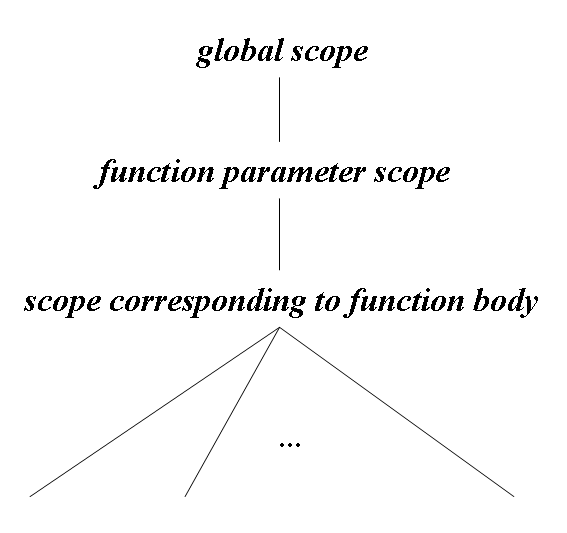
\includegraphics[width=0.5\linewidth,height=0.5\linewidth]{traverse_e.png}
%% \end{htmlonly}
%% \begin{latexonly}
%% 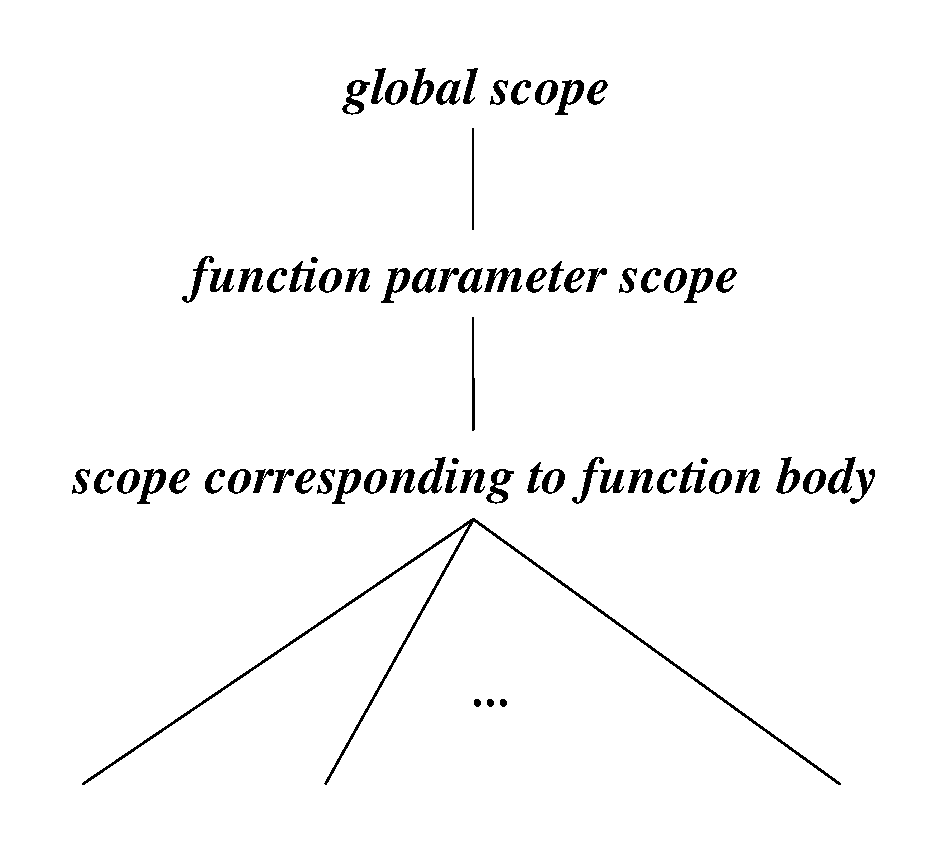
\includegraphics[width=0.5\linewidth,height=0.5\linewidth]{traverse_e.eps}
%% \end{latexonly}
%% \caption{Symbol table outputed by frontend to backend}
%% \label{speed_e000}
%% \end{center}
%% \end{figure}
%% 
%% Every scope except for ``global scope'' in figure \ref{speed_e000}
%% is outputed to backend differently with any time.
%% On the other hand, ``global scope'' becomes grater than
%% previous time. If a big translation unit (file) is
%% compiled, ``global scope'' increases.
%% 
%% Now, we want to deal with ``global scope'' specially.
%% Frontend prepares a container where only new entries exists,
%% backend referenses it like bellow.
%% \begin{verbatim}
%% // Frontend : Container for only new entries added into global scope.
%% vector<usr*> new_external_declaration;
%% 
%% // Frontend : routine for adding into symbol table
%% void add_symtab(usr* entry)
%% {
%%   string name = entry->m_name;
%%   map<string, vector<var*> >& usrs = scope::current->m_usr;
%%   usrs[name].push_back(entyr);
%%   if ( scope::current == &scope::root ) {
%%     // added into global scope
%%     new_external_declaration.push_back(entry);
%%   }
%% }
%% 
%% // Frontend : Yacc action function when grammer symbol
%% // `function-definition' is reduced.
%% void function_definition(comp_stmt* cs)
%% {
%%   cs->gen();  // 3 address codes are outputed in global
%%               // container `code'
%%   ...
%%   
%%   // Output symbol table, 3 address codes and new entries added
%%   // in global scope to backend
%%   backend(&scope::root,code,new_external_declaration,...);
%%   ...
%%   new_external_declaration.clear(); // Clear here.
%% }
%% 
%% // Backend : traverse symbol table
%% void traverse(scope* ptr)
%% {
%%   if ( ptr == &scope::root ) {
%%     // Global scope. Specially reference the container
%%     const vector<usr*>& v = new_external_declaration;
%%     for_each(v.begin(),v.end(),...);
%%   }
%%   else {
%%     // Not global scope. Normally reference symbol table.
%%     map<string, usr*>& usrs = ptr->m_usrs;
%%     for_each(usrs.begin(),usrs.end(),...);
%%     ...
%%   }
%%   vector<scope*>& children = ptr->m_children;
%%   for_each(children.beign(),children.end(),traverse);
%% }
%% \end{verbatim}
%% Internally, backend may have the table which converts `{\tt{var}}' to
%% address descriptor. In such an implementaion, the table should be
%% parted into permanent table and temporary table like bellow.
%% \begin{verbatim}
%% // Table converting var to address descriptor
%% typedef map<var*, address*> addr_desc;
%% 
%% pair<addr_desc,addr_desc> address_descriptors;
%% // Use address_descriptors.first as permanent and
%% // address_descriptors.second as temporary
%% \end{verbatim}

\section{{\tt{dynamic\_cast}}}

We use {\tt{C++}} language for implementing {\tt{C}} compiler.
And we use {\tt{dynamic\_cast}} in some situations.
Please remember that
this operator is very expensive judging from compile speed.



\chapter{Optimization}

\label{optimize_e051}

We've discussed how frontend generates symbol table and 3 address codes
from C program text until chapter \ref{stmt_e006}. In this chapter,
we'll discuss how frontend generates better symbol table and 3 address codes.

As we described at chapter \ref{stmt_e006},
when grammer symbol {\tt{function-definition}} is reduced
while bottom-up parsing, symbol table and 3 address codes are obtained
like bellow.

\begin{verbatim}
%{
/* yacc program text */
vector<tac*> code;
struct scope {
  ...
  static scope root;
};
%}

%%
...
function_definition
  : function_header compound_statement
    { function_definition($2); }
...
%%
void function_definition(comp_stmt* cs)
{
  cs->gen(); /* Genereate 3 address codes into global container `code' */
  ...
  if ( !error::counter )
    optimize(code);

  backend(&scope::root,code,...);  // Output symbol table and
                                   // 3 address codes to backend.
  ...
}
\end{verbatim}

\section{Unreferenced label}
\label{optimize_e003}
At \ref{_3ac_e002}, label are expressed class `{\tt{to3ac}}'
which contains referencing jump code in the member `{\tt{to3ac::m\_goto}}'.
So, we can easily know whether the label is referenced or not.
And if not, the label is erased like bellow.
\begin{verbatim}
void erase_to3ac(vector<tac*>& v)
{
  for ( p = v.begin() ; p != v.end() ; ) {
    to3ac* to = dynamic_cast<to3ac*>(*p);
    if ( !to ) {
      ++p;
      continue; 
    }
    if ( !to->m_goto.empty() ) {
      ++p;
      continue; 
    }
    p = v.erase(p);
  }
}
\end{verbatim}

\section{Basic block optimization}
\label{optimize_e058}
Chapter 9 of bibliography \cite{doragon} says about 
the way of basic block optimization. Basic block
is expressed like bellow.
\begin{verbatim}
struct basic_block {
  tac** m_leader;                  // Leader of this basic block
  int m_size;                      // Size of this basic block
  vector<basic_block*> m_preceed;  // Preceed basic blocks
  vector<basic_block*> m_follow;   // Following basic blocks
};
\end{verbatim}

\subsection{Division into basic blocks}

Bibliography \cite{doragon} algorithm 9.1 says about 
division into basic blocks. Now here, If the 3 address
code is one of {\tt{return}}, {\tt{call}},
and {\tt{*y := z}}, we additionally
make it  a leader of basic block.
For example,
\begin{verbatim}
int f(int* a, int* b, int n)
{
  int prod = 0;
  for ( int i = 0 ; i < n ; ++i )
    prod += a[i] * b[i];
  return prod;
}
\end{verbatim}
for above program, 3 address codes become like bellow.
\begin{verbatim}
f:
    prod := 0
    i := 0
  label0:
    if i >= n goto label1
    t0 := 4 * i
    t1 := a + t0
    t2 := 4 * i
    t3 := b + t2
    t4 := *t1
    t5 := *t3
    t6 := t4 * t5
    t7 := prod + t6
    prod := t7
    i := i + 1
    t8 := i
    goto label0
  label1:
    t9 := prod
    return t9
\end{verbatim}
These 3 address codes are devided into basic blocks illustrated
figure \ref{optimize_e000}.
\begin{figure}[htbp]
\begin{center}
%%\begin{htmlonly}
%%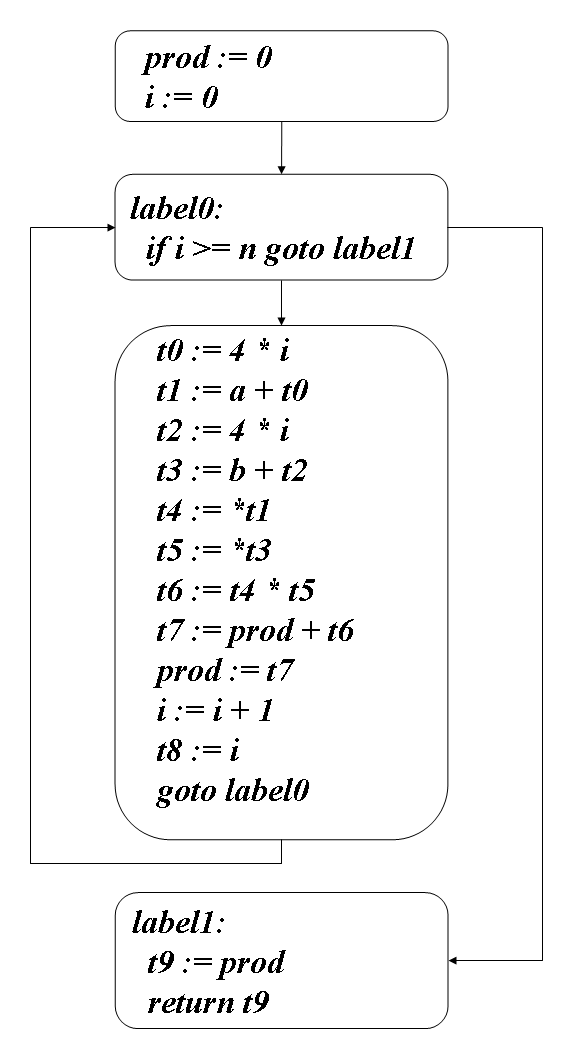
\includegraphics[width=0.8\linewidth,height=1.436\linewidth]{basic_block.png}
%%\end{htmlonly}
%%\begin{latexonly}
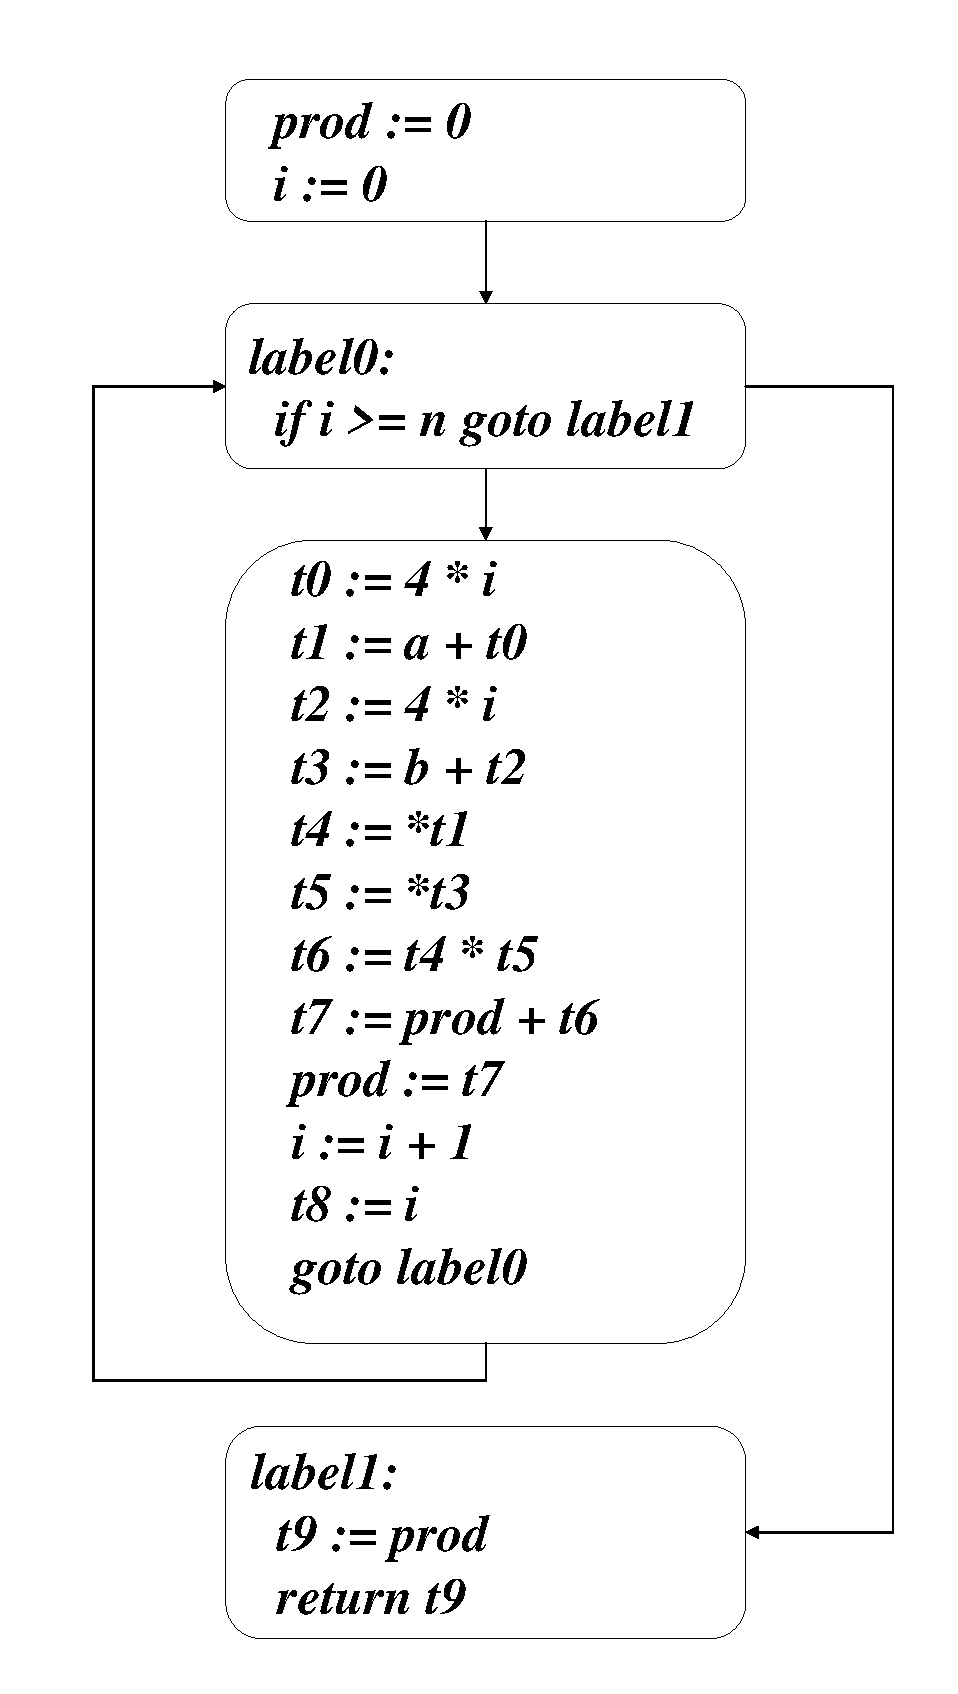
\includegraphics[width=0.8\linewidth,height=1.436\linewidth]{basic_block.eps}
%%\end{latexonly}
\caption{Division into basic blocks}
\label{optimize_e000}
\end{center}
\end{figure}

\subsection{Alive medium variable beyond basic block}

\label{optimize_e004}
Bibliography \cite{doragon} 9.5 says like bellow.
\begin{quote}
However if medium code generation algorithm or optimization algorithm
uses the same temporary variables through some basic blocks,
it is necessary to assume that they are alive beyond the basic blocks.
For this, mark such temporary variables specially, and distinguish
alive or death of temporary variables.
\end{quote}
Here, let's think about the medium variable which is alive beyond
basic block and is generated by the algorithm discussed in \ref{expr_e000}.
For example,
\begin{verbatim}
int f(int a, int b, int c){ return a * b + !c; }
\end{verbatim}
for this program, 3 address codes become like bellow.
\begin{verbatim}
f:
  t0 := a * b
  if c != 0 goto label1
  t1 := 1
  goto label2
label1:
  t1 := 0
label2
  t2 := t0 + t1
  return t2
\end{verbatim}
These 3 address codes are diveded into basic block illustrated in
figure \ref{optimize_e001}.
\begin{figure}[htbp]
\begin{center}
%%\begin{htmlonly}
%%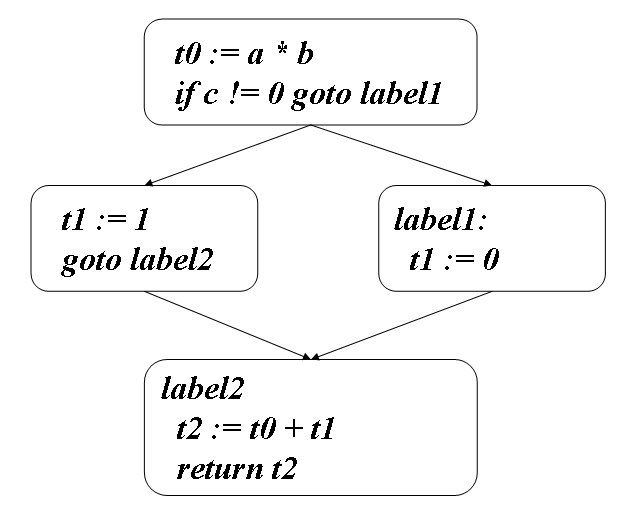
\includegraphics[width=0.89\linewidth,height=1.0\linewidth]{beyond_medium.png}
%%\end{htmlonly}
%%\begin{latexonly}
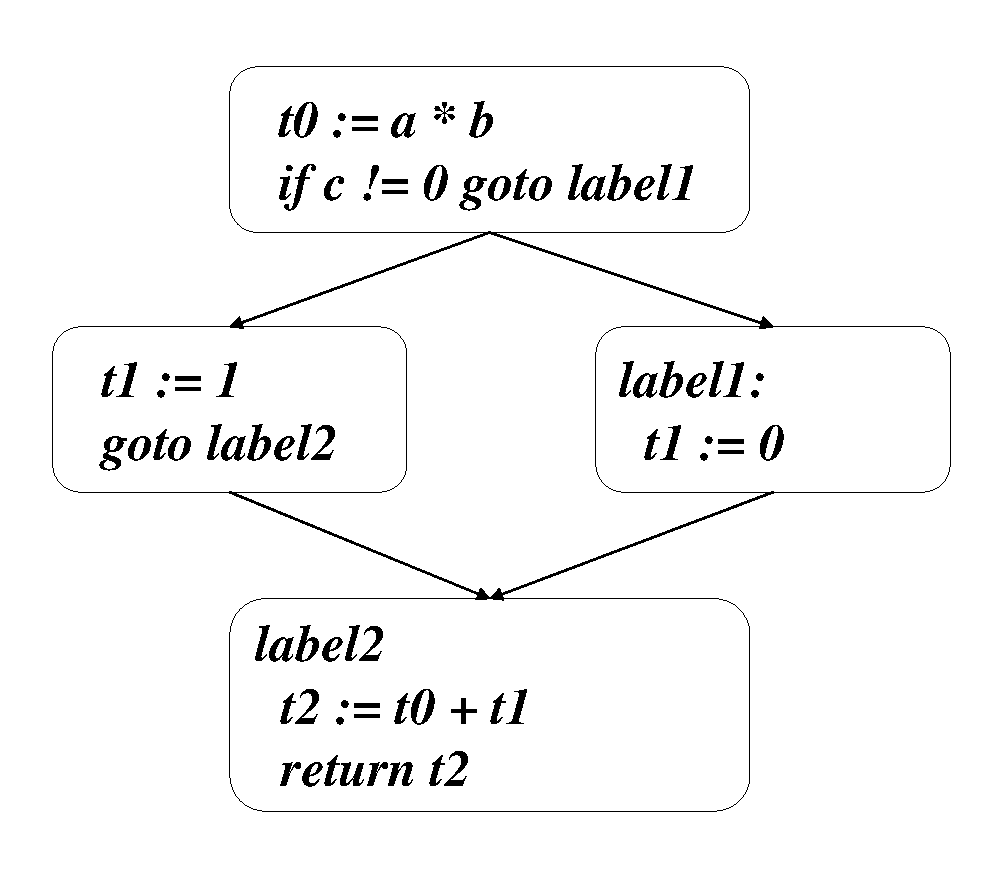
\includegraphics[width=0.89\linewidth,height=1.0\linewidth]{beyond_medium.eps}
%%\end{latexonly}
\caption{Alive medium variable beyond basic block}
\label{optimize_e001}
\end{center}
\end{figure}
`{\tt{t1}}' is alive beyond basic blocks. And please
note that `{\tt{t0}}' is also alive beyond basic blocks.
Generally, for binary operator $@$ and expression $expr_0 @ expr_1$,
if the result of $expr_1$ is alive beyond basic blocks,
then the result of $expr_0$ is also  alive beyond basic blocks.
\begin{verbatim}
void bin_expr::eval(expr* left, expr* right)
{
  var* y = left->eval();
  y = y->rvalue();
  var* z = right->eval();
  z = z->rvalue();
  if ( z->m_beyond ) {
    // Marked specially. i.e. `z' is alive beyond basic blocks.
    // Now mark `y' specially.
    y->m_beyond = true;
  }
  ...
  var* x = y->vf(z);
  ...
  return x;
  // `x' is not still marked specially. But if some operator is
  // applied to `x', it may be marked specially. i.e. We cannot
  // assume `x' is not alive beyond basic block.
}
\end{verbatim}
If frontend doesn't analize alive variables which are in program text
and frontend assumes that they are alive beyond basic blocks,
frontend has to assume that all medium variables may be alive beyond
basic block. That is, all medium variables are marked specially and
they are alive beyond basic blocks.

\subsection{Analisis alive variables}

Bibliography \cite{doragon} algorithm 10.4 says about 
analisis alive variables, and here, we'll take this way.
Consider bellow program please.
\begin{verbatim}

extern int a[];

void quicksort(int m, int n)
{
  if ( n <= m ) return;
  int i = m - 1;
  int j = n;
  int v = a[n];
  while ( 1 ) {
    do i = i + 1; while ( a[i] < v );
    do j = j - 1; while ( a[j] > v );
    if ( i >= j ) break;
    int x = a[i]; a[i] = a[j]; a[j] = x;
  }
  int y = a[i]; a[i] = a[n]; a[n] = y;
  quicksort(m,j); quicksort(i+1,n);
}
\end{verbatim}
For this program, generate symbol table and 3 addres codes
and then erase unreferenced label described in \ref{optimize_e003},
3 address codes become like bellow.
\begin{verbatim}
quicksort:                  label4:
  if n > m goto label0        t10 := 4 * i
  return                      t11 := a[t10]
label0:                       x := t11
  t0 := m - 1                 t12 := 4 * i
  i := t0                     t13 := 4 * j
  t1 := n                     t14 := a[t13]
  j := t1                     a[t12] := t14
  t2 := 4 * n                 t15 := 4 * j
  t3 := a[t2]                 t16 := x
  v := t3                     a[t15] := t16
label1:                       goto label1
label2:                     label5:
  t4 := i + 1                 t17 := 4 * i
  i := t4                     t18 := a[t17]
  t5 := 4 * i                 y := t18
  t6 := a[t5]                 t19 := 4 * i
  if t6 < v goto label2       t20 := 4 * n
label3:                       t21 := a[t20]
  t7 := j - 1                 a[t19] := t21
  j := t7                     t22 := 4 * n
  t8 := 4 * j                 t23 := y
  t9 := a[t8]                 a[t22] := t23
  if t9 > v goto label3       t24 := m
  if i < j goto label4        t25 := j
  goto label5                 param t24
                              param t25
                              call quicksort
                              t26 := i + 1
                              t27 := n
                              param t26
                              param t27
                              call quicksort
\end{verbatim}
These 3 address codes are dived into basic blocks illustrated in
figure \ref{optimize_e002}.
\begin{figure}[htbp]
\begin{center}
%%\begin{htmlonly}
%%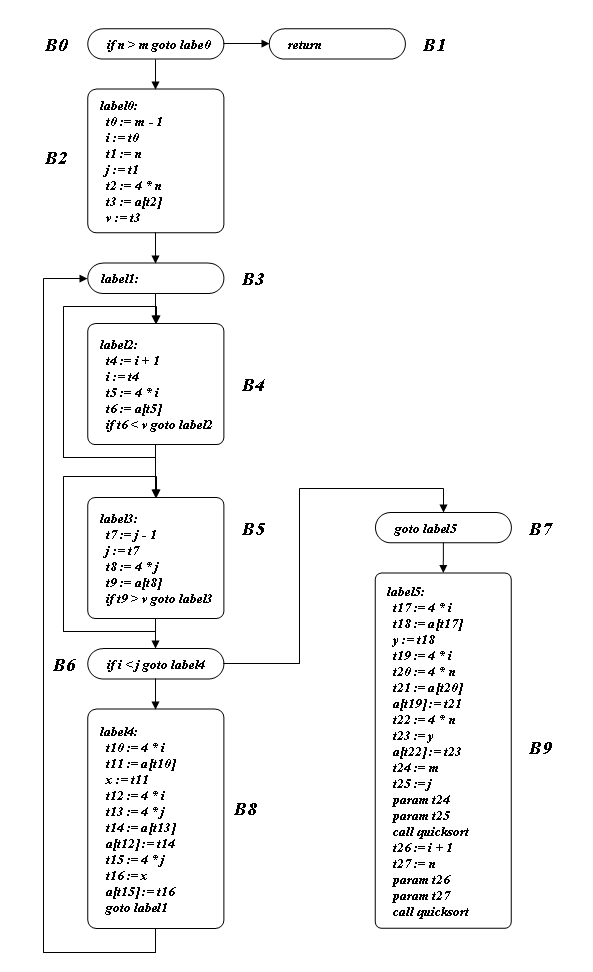
\includegraphics[width=1.01\linewidth,height=1.75\linewidth]{quicksort.png}
%%\end{htmlonly}
%%\begin{latexonly}
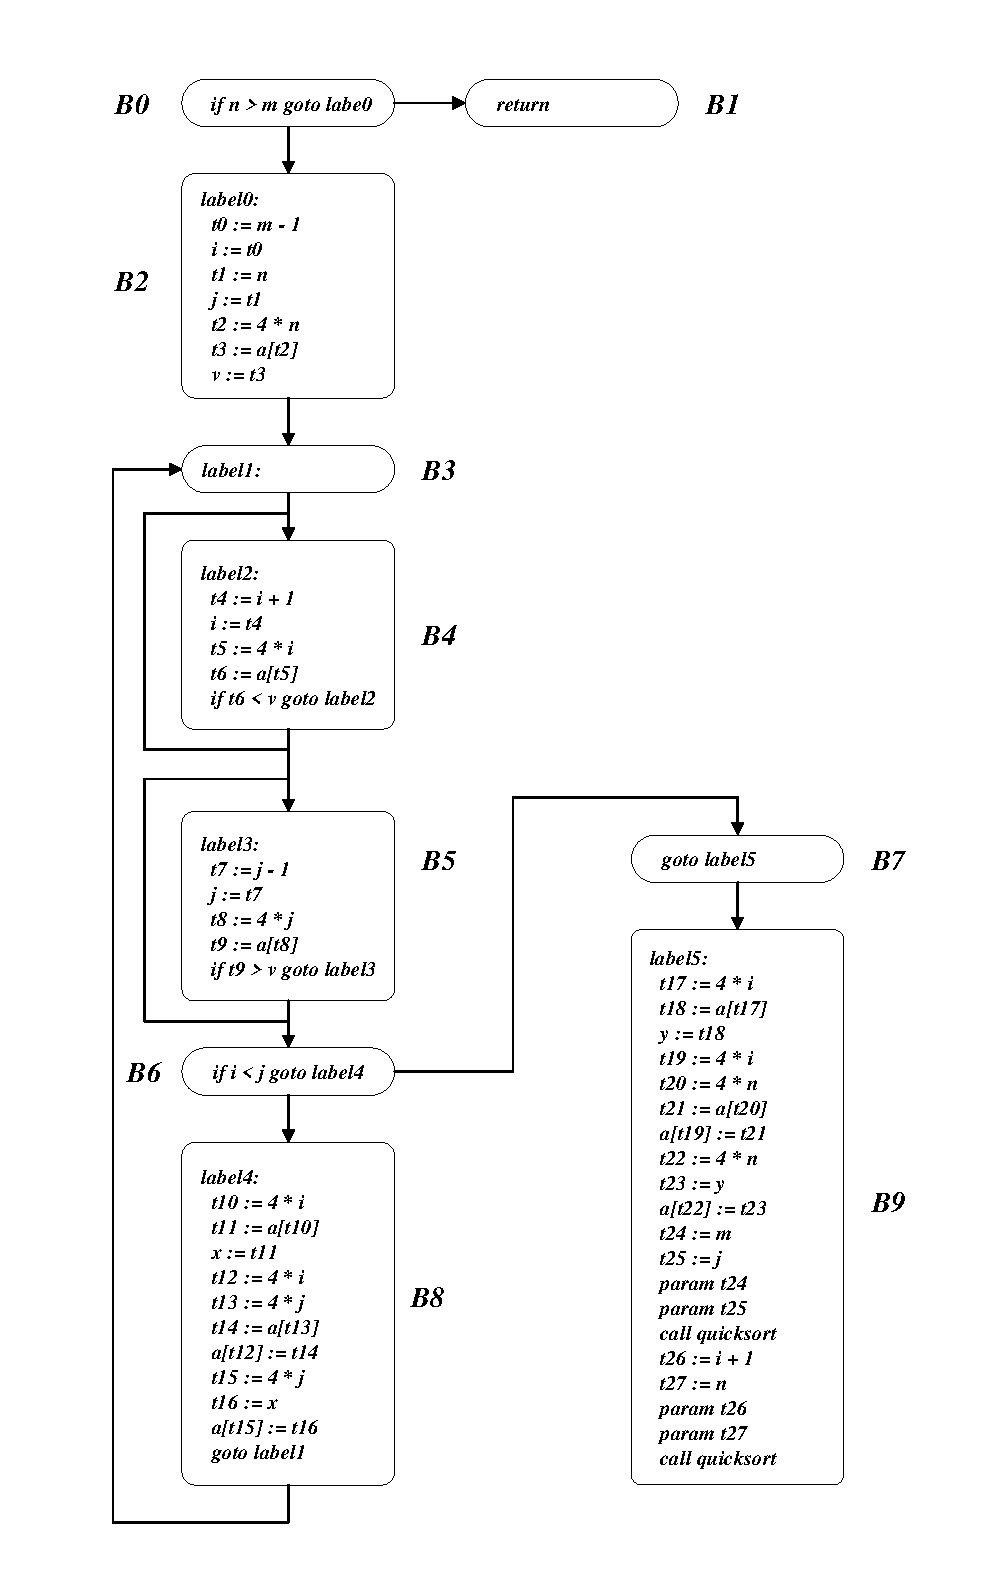
\includegraphics[width=1.01\linewidth,height=1.75\linewidth]{quicksort.eps}
%%\end{latexonly}
\caption{basic blocks of {\tt{quicksort}}}
\label{optimize_e002}
\end{center}
\end{figure}
It is possible that there are medium varialbes which is alive beyond
basic blocks in \ref{optimize_e004}. But as far as this code, there is
no any medium variable which is alive beyond basic block.
This fact is led by bellow algorithm.

Let $in[B]$ denote set of alive variables in the entrance of
basic block $B$. Samely, let $out[B]$ denote set of alive
variables in an exit of basic block $B$. Let $def[B]$ denote
set of variables which is defined before usage in basic
block $B$ and let $use[B]$ denote set of variables which is used before
definition. As described in bibliography \cite{doragon} expression
(10.11), the folloing equations holds.
\begin{eqnarray*}
out[B] & = & \bigcup_{F {\tt{\,\,follows\,\,} B}} in[F] \\
in[B]  & = & use[B] \cup (out[B] - def[B])
\end{eqnarray*}
Now our aim is to get $out$, and repeat method 
is available for solve these equations as described in bibliography
\cite{doragon}.

First, for each basic block in figure \ref{optimize_e002},
calcurate $def, use$. They become like bellow.

\vspace{0.5cm}

\begin{tabular}{|l|l|l|} \hline
   & $def$             & $use$     \\ \hline
B0 &                   & m n       \\ \hline
B1 &                   &           \\ \hline
B2 & v i j t0 t1 t2 t3 & a m n 1 4 \\ \hline
B3 &                   &           \\ \hline
B4 & t4 t5 t6          & a v i 1 4 \\ \hline
B5 & t7 t8 t9          & a v j 1 4 \\ \hline
B6 &                   & i j       \\ \hline
B7 &                   &           \\ \hline
B8 & x t10 t11 t12 t13 t14 t15 t16 & a i j 4 \\ \hline
B9 & y t17 t18 t20 t19 t21 t22 t23 & quicksort a m n \\
   & t24 t25                & i j 4 \\ \hline
B10 & t26 t27 & quicksort n i 1 \\ \hline
\end{tabular}

\vspace{0.5cm}

Generally, global variables are alive in every basic block, so
add them into every $out[B]$.

For each $B$, make $in[B]$ an empty set and 
start repeat method.

\vspace{0.5cm}

\begin{tabular}{|l|l|l|} \hline
step 0  & $out$             & $in$      \\ \hline
B0 & quicksort a 1 4   & quicksort a 1 4 m n \\ \hline
B1 & quicksort a 1 4   & quicksort a 1 4     \\ \hline
B2 & quicksort a 1 4   & quicksort a 1 4 m n \\ \hline
B3 & quicksort a 1 4   & quicksort a 1 4     \\ \hline
B4 & quicksort a 1 4   & quicksort a 1 4 v i \\ \hline
B5 & quicksort a 1 4   & quicksort a 1 4 v j \\ \hline
B6 & quicksort a 1 4   & quicksort a 1 4 i j \\ \hline
B7 & quicksort a 1 4   & quicksort a 1 4     \\ \hline
B8 & quicksort a 1 4   & quicksort a 1 4 i j \\ \hline
B9 & quicksort a 1 4 \hspace{1.7cm}
 & quicksort a 1 4 m n i j  \hspace{0.1cm} \\ \hline
\end{tabular}

\begin{tabular}{|l|l|l|} \hline
step 1  & $out$             & $in$      \\ \hline
B0 & quicksort a 1 4 m n     & quicksort a 1 4 m n   \\ \hline
B1 & quicksort a 1 4 m n     & quicksort a 1 4 m n   \\ \hline
B2 & quicksort a 1 4         & quicksort a 1 4 m n   \\ \hline
B3 & quicksort a 1 4 v i     & quicksort a 1 4 v i j \\ \hline
B4 & quicksort a 1 4 v i j   & quicksort a 1 4 v i j \\ \hline
B5 & quicksort a 1 4 v i j   & quicksort a 1 4 v i j \\ \hline
B6 & quicksort a 1 4 i j     & quicksort a 1 4 i j   \\ \hline
B7 & quicksort a 1 4 m n i j & quicksort a 1 4 m n i j  \\ \hline
B8 & quicksort a 1 4 v i     & quicksort a 1 4 v i j  \\ \hline
B9 & quicksort a 1 4  \hspace{1.7cm}
   & quicksort a 1 4 m n i j  \hspace{0.1cm} \\ \hline
\end{tabular}

\begin{tabular}{|l|l|l|} \hline
step 2  & $out$             & $in$      \\ \hline
B0 & quicksort a 1 4 m n       & quicksort a 1 4 m n        \\ \hline
B1 & quicksort a 1 4 m n       & quicksort a 1 4 m n        \\ \hline
B2 & quicksort a 1 4 v i       & quicksort a 1 4 m n        \\ \hline
B3 & quicksort a 1 4 v i j     & quicksort a 1 4 v i j      \\ \hline
B4 & quicksort a 1 4 v i j     & quicksort a 1 4 v i j      \\ \hline
B5 & quicksort a 1 4 v i j     & quicksort a 1 4 v i j      \\ \hline
B6 & quicksort a 1 4 v m n i j & quicksort a 1 4 v m n i j  \\ \hline
B7 & quicksort a 1 4 m n i j   & quicksort a 1 4 m n i j  \\ \hline
B8 & quicksort a 1 4 v i j     & quicksort a 1 4 v i j  \\ \hline
B9 & quicksort a 1 4           & quicksort a 1 4 m n i j \\ \hline
\end{tabular}

\begin{tabular}{|l|l|l|} \hline
step 3  & $out$             & $in$      \\ \hline
B0 & quicksort a 1 4 m n       & quicksort a 1 4 m n        \\ \hline
B1 & quicksort a 1 4 m n       & quicksort a 1 4 m n        \\ \hline
B2 & quicksort a 1 4 v i j     & quicksort a 1 4 m n        \\ \hline
B3 & quicksort a 1 4 v i j     & quicksort a 1 4 v i j      \\ \hline
B4 & quicksort a 1 4 v i j     & quicksort a 1 4 v i j      \\ \hline
B5 & quicksort a 1 4 v m n i j & quicksort a 1 4 v m n i j  \\ \hline
B6 & quicksort a 1 4 v m n i j & quicksort a 1 4 v m n i j  \\ \hline
B7 & quicksort a 1 4 m n i j   & quicksort a 1 4 m n i j  \\ \hline
B8 & quicksort a 1 4 v i j     & quicksort a 1 4 v i j  \\ \hline
B9 & quicksort a 1 4           & quicksort a 1 4 m n i j \\ \hline
\end{tabular}

\begin{tabular}{|l|l|l|} \hline
step 4  & $out$             & $in$      \\ \hline
B0 & quicksort a 1 4 m n       & quicksort a 1 4 m n        \\ \hline
B1 & quicksort a 1 4 m n       & quicksort a 1 4 m n        \\ \hline
B2 & quicksort a 1 4 v i j     & quicksort a 1 4 m n        \\ \hline
B3 & quicksort a 1 4 v i j     & quicksort a 1 4 v i j      \\ \hline
B4 & quicksort a 1 4 v m n i j & quicksort a 1 4 v m n i j  \\ \hline
B5 & quicksort a 1 4 v m n i j & quicksort a 1 4 v m n i j  \\ \hline
B6 & quicksort a 1 4 v m n i j & quicksort a 1 4 v m n i j  \\ \hline
B7 & quicksort a 1 4 m n i j   & quicksort a 1 4 m n i j  \\ \hline
B8 & quicksort a 1 4 v i j     & quicksort a 1 4 v i j  \\ \hline
B9 & quicksort a 1 4           & quicksort a 1 4 m n i j \\ \hline
\end{tabular}

\begin{tabular}{|l|l|l|} \hline
step 5  & $out$             & $in$      \\ \hline
B0 & quicksort a 1 4 m n       & quicksort a 1 4 m n        \\ \hline
B1 & quicksort a 1 4 m n       & quicksort a 1 4 m n        \\ \hline
B2 & quicksort a 1 4 v i j     & quicksort a 1 4 m n        \\ \hline
B3 & quicksort a 1 4 v m n i j & quicksort a 1 4 v m n i j  \\ \hline
B4 & quicksort a 1 4 v m n i j & quicksort a 1 4 v m n i j  \\ \hline
B5 & quicksort a 1 4 v m n i j & quicksort a 1 4 v m n i j  \\ \hline
B6 & quicksort a 1 4 v m n i j & quicksort a 1 4 v m n i j  \\ \hline
B7 & quicksort a 1 4 m n i j   & quicksort a 1 4 m n i j  \\ \hline
B8 & quicksort a 1 4 v m n i j & quicksort a 1 4 v m n i j  \\ \hline
B9 & quicksort a 1 4           & quicksort a 1 4 m n i j \\ \hline
\end{tabular}

\begin{tabular}{|l|l|l|} \hline
step 6  & $out$             & $in$      \\ \hline
B0 & quicksort a 1 4 m n       & quicksort a 1 4 m n        \\ \hline
B1 & quicksort a 1 4 m n       & quicksort a 1 4 m n        \\ \hline
B2 & quicksort a 1 4 v i j     & quicksort a 1 4 m n        \\ \hline
B3 & quicksort a 1 4 v m n i j & quicksort a 1 4 v m n i j  \\ \hline
B4 & quicksort a 1 4 v m n i j & quicksort a 1 4 v m n i j  \\ \hline
B5 & quicksort a 1 4 v m n i j & quicksort a 1 4 v m n i j  \\ \hline
B6 & quicksort a 1 4 v m n i j & quicksort a 1 4 v m n i j  \\ \hline
B7 & quicksort a 1 4 m n i j   & quicksort a 1 4 m n i j  \\ \hline
B8 & quicksort a 1 4 v m n i j & quicksort a 1 4 v m n i j  \\ \hline
B9 & quicksort a 1 4           & quicksort a 1 4 m n i j \\ \hline
\end{tabular}

\vspace{0.5cm}
For each basic block $B$, $in[B]$ of step 5 is equal to that of step 6.
So the repeat method is finished.

For each basic block $B$ in figure \ref{optimize_e002},
$out[B]$ becomes like bellow.

\vspace{0.5cm}

\begin{tabular}{|l|l|l|} \hline
   & $out$                            \\ \hline
B0 & quicksort a m n  1 4             \\  \hline
B1 & quicksort a 1 4                  \\ \hline
B2 & quicksort a m n  v i j 1 4       \\ \hline
B3 & quicksort a m n  v i j 1 4       \\ \hline
B4 & quicksort a m n  v i j 1 4       \\ \hline
B5 & quicksort a m n  v i j 1 4       \\ \hline
B6 & quicksort a m n  v i j 1 4       \\ \hline
B7 & quicksort a m n    i j 1 4       \\ \hline
B8 & quicksort a m n  v i j 1 4       \\ \hline
B9 & quicksort a 1 4              \\ \hline
\end{tabular}

\vspace{0.5cm}

Similally, for figure \ref{optimize_e001},
this algorithm tell us that
`{\tt{t0}}' and `{\tt{t1}}'
are in $out[B]$ for every basic block $B$, except for last basic block.

\subsection{Assignment and common expression}
\label{optimize_e_assign}
We've discussed about how to devide into basic block
and how to analize alive variable until previous section. Now here, 
we'll think about how to detect redundant assignment and common
expression from 3 address codes.

We'll express basic block with {\em dag} described in bibliography
 \cite{doragon}. {\em dag} is like bellow structure.

\begin{verbatim}
struct dag {  // Node of dag
  tac* m_tac;        // Correspond 3 address code. Label of this node.
  vector<var*> m_vars;      // Calcurating variables. Identifier list.
  vector<dag*> m_parents;   // Parent
  dag* m_left;              // Left child
  dag* m_right;             // Right child
  dag* m_extra;             // 3rd child for `x' of x[y] := z
  static vector<dag*> all;  // All list
  dag() : m_tac(0), m_left(0), m_right(0) { all.push_back(this); }
};

map<var*, dag*> node;  // Table from variable to node.
\end{verbatim}

Before showing conversion from basic block to {\em dag},
or corresponding code generation algorithm,
let's think about bellow simple example.

\begin{Example}
\label{optimize_e006}
\begin{verbatim}
int n; void f(void){ ++n; }
\end{verbatim}
3 address codes become like bellow.
\begin{verbatim}
f:
   n := n + 1
  t0 := n
\end{verbatim}
Figure \ref{optimize_e005} illustrates
process of creating {\em dag} from these 3 address codes.
\begin{figure}[htbp]
\begin{center}
%%\begin{htmlonly}
%%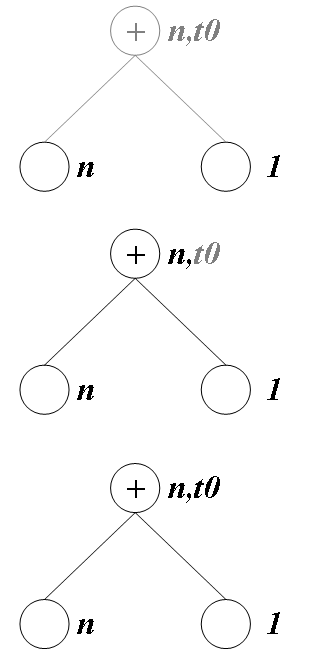
\includegraphics[width=0.5\linewidth,height=1.01\linewidth]{opt000.png}
%%\end{htmlonly}
%%\begin{latexonly}
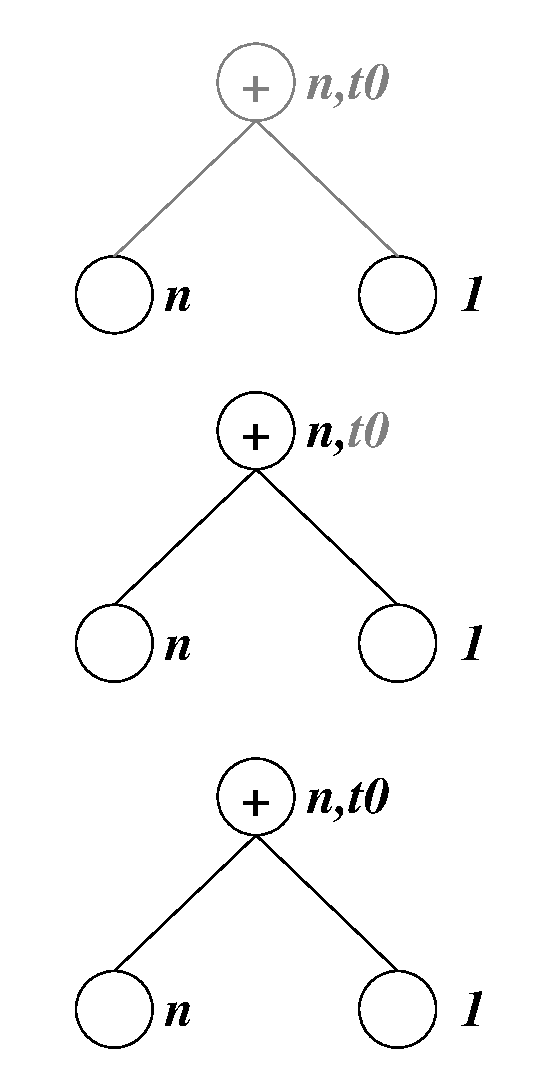
\includegraphics[width=0.5\linewidth,height=1.01\linewidth]{opt000.eps}
%%\end{latexonly}
\caption{{\em dag} of example \ref{optimize_e006}}
\label{optimize_e005}
\end{center}
\end{figure}

\begin{enumerate}
\item At {\tt{n := n + 1}}, for right hand `{\tt{n}}', 
{\tt{node[n]}} is not defined, so create new node. And
add `{\tt{n}}' into identifier list {\tt{m\_vars}}.
Finally make this {\tt{dag}} {\tt{node[n]}}.

\item At {\tt{n := n + 1}}, for `{\tt{1}}' ,
 {\tt{node[1]}} is not defioned, so create new node. And 
add `{\tt{1}}' into identifier list {\tt{m\_vars}}.
Finally make this {\tt{dag}} {\tt{node[1]}}.

\item From {\tt{dag::all}}, find the node whose label is `{\tt{+}}'
and whose left child is equal to {\tt{node[n]}}
and whose right child is equal to {\tt{node[1]}}.
There is not such a node, so create {\tt{dag}}  and
make it satisfying the condition.
And make this {\tt{dag}} {\tt{node[n]}}.

\item At {\tt{t0 := n}}, for `{\tt{n}}',
{\tt{node[n]}} is already defined.
Add `{\tt{t0}}' into identifier list {\tt{m\_vars}} of {\tt{node[n]}}.
\end{enumerate}
After constructing {\em dag}, generate 3 address codes by evaluating
in order.

\begin{enumerate}
\item Evaluate the node whose identifier list is `{\tt{n}}'.
      Here no code is generated. The result is `{\tt{n}}'.

\item Evaluate the node whose identifier list is `{\tt{1}}'.
      Here no code is generated. The result is `{\tt{1}}'.

\item Evaluate the node whose identifier list is `{\tt{n, t0}}'.
      Find identifer $x$ from identifier list, where {\tt{node[$x$]}} is equal
      to this node and $x$ is alive in an exit of basic block.
      Here we chose `{\tt{n}}'.
      And generate code {\tt{n := n + 1}}.
 
\item For the other element of identifier list, if the identifier
      is alive in an eit of basic block, generate assignment code.
      In this case, {\tt{t0}} is not alive in an exit of this
      basic block.

\end{enumerate}
At last, {\tt{n := n + 1}} is only generated.
\end{Example}

We can get {\em dag} of basic block by bellow algorithm.

\begin{quote}
{\bf Creation {\em dag} of basic block algorithm}

For each 3 address code of basic block, apply bellow. 
\begin{enumerate}
\item For {\tt{x := y $op$ z}}, if {\tt{y}} is not specified,
      the 3 address code is special like 
      return without return value
      ({\tt{return3ac::y}} is 0),
      unconditional jump ({\tt{goto3ac::y}} is 0),
      label ({\tt{to3ac}}) or
      assembly output({\tt{asm3ac}}).
      In this case, create new node and terminate this procedure. 

\item If {\tt{node[y]}} is not still defined, 
      create new node and add {\tt{y}} into its {\tt{m\_vars}}.
      Make this dag {\tt{node[y]}}. 

\item If {\tt{z}} is specified and {\tt{node[z]}} is not still defined,
      create new node and add {\tt{z}} into its {\tt{m\_vars}}.
      Make this dag {\tt{node[z]}}.

\item 
\label{optimize_e047}
Get node $n$ like bellow.

\begin{enumerate}
\item If the 3 address code is {\tt{x := y}},
      let {\tt{node[y]}} to be $n$.
\item If the 3 address code is {\tt{call}} or {\tt{va\_arg}},
      create new node and let it to be $n$.
\item For {\tt{x := y $op$ z}}, if {\tt{x}} is not specified,
      create new node and let it to be $n$.
\item For 3 address code {\tt{x := y $op$ z}} expcet for above,
      find from {\tt{dag::all}} the node 
      whose left child is {\tt{node[y]}},
      whose right child is {\tt{node[z]}}
      and
      whose label is $op$. Especially,
\begin{enumerate}
\item In case of {\tt{x := y[z]}}, {\tt{x := *y}},
      type of {\tt{x}} must be {\it
      compatible}.
\item In case of {\tt{x[y] := z}}, {\tt{alloca x, y}},
      {\tt{x}} must be equal.
\item In case of {\tt{x := (type)y}}, {\tt{type}} must be
     {\it compatible}.
\end{enumerate}
      If exists, let it to be $n$.
\item \label{optimize_e109}
      If there is not such a node and in case of {\tt{x := y[z]}},
      find from {\tt{dag::all}} the node like bellow.
      \begin{itemize}
      \item label is {\tt{x'[y'] := z'}}.
      \item {\tt{node[y]}} is equal to the node.
      \item {\tt{node[z]}} is equal to left child of the node.
      \item type of {\tt{x}} is {\it compatible} with that of {\tt{z'}}.
      \end{itemize}
      If exists, let its right child to be $n$.
\item \label{optimize_e064}
If there is not such a node, create new node and let it to be $n$.
For {\tt{x[y] := z}}, if {\tt{node[x]}} already exists, let {\tt{node[x]}}
to be 3rd child of $n$.
\end{enumerate}
\item \label{optimize_e112}
      If this 3 address code is {\tt{call3ac} or {\tt{invladdr3ac}}},
      apply bellow and terminate this procedure.
      \begin{enumerate}
      \item If this 3 address code is {\tt{x := call f}} and {\tt{x}} 
            is not 0, add {\tt{x}} into {\tt{m\_vars}} of $n$ and
            update {\tt{node[x]}} to be $n$. 
      \item Apply {\bf Code generation algorithm from {\em dag}}
	    described bellow.
      \item Clear {\tt{node}}.
      \item Clear {\tt{result}} described bellow.
      \end{enumerate}

\item For 3 address code {\tt{x := y $op$ z}}, if {\tt{x}} is not specified,
      terminate this procedure.

\item Add {\tt{x}} of 3 address code {\tt{x := y op z}} into
      {\tt{m\_vars}} of $n$ which is gotten in \ref{optimize_e047}.
      And update {\tt{node[x]}} to be $n$. 
\end{enumerate}

\end{quote}

For generating code from {\em dag}, apply bellow.

\begin{quote}
{\bf Code generation algorithm from {\em dag}}

For each node of {\tt{dag::all}}, apply bellow procedure which returns
{\tt{var*}}. And keep the result of this procedure in
{\tt{map<dag*, var*> result}}.

\begin{enumerate}
\item If the label of the node is none, call bellow procedure
      {\bf Assignment judge algorithm} and return it.

\item \label{optimize_e048}
      Let {\tt{x := y $op$ z}} denote the label.
      For the left child $\ell$, replace `{\tt{y}}' with
      {\tt{result[$\ell$]}}.
\item \label{optimize_e049}
      Simillary, for the right child $r$, replace `{\tt{z}}'
      with {\tt{result[$r$]}}.
\item \label{optimize_e050}
      Copy the 3 address code {\tt{x := y $op$ z}} to the container
      for optimization result, where {\tt{y}} and {\tt{z}}
      is obtained in \ref{optimize_e048}, \ref{optimize_e049}.
\item Update `{\tt{x}}' of {x := y $op$ z} which is copied in
      \ref{optimize_e050} appling bellow procedure
      {\bf Assignment judge algorithm}. Now we'll refere updated
       {\tt{x}} as just `{\tt{x}}'.
\item  If `{\tt{x}}' is zero or this node has a parent or parents,
       return `{\tt{x}}'.
\item If `{\tt{x}}' is alive in an exit of this basic block,
      return `{\tt{x}}'.
\item If `{\tt{x}}' is used before it is defined
      in this basic block, and {\tt{node[x]}} is equal to
      the current {\tt{dag}}, return `{\tt{x}}'.
\item For `{\tt{x}}', if there exists a 3 address code {\tt{p := \&x}} in this
      basic block, return `{\tt{x}}'.
\item \label{optimize_e057}
      If a 3 address code copied at \ref{optimize_e050} is
      {\tt{x := call y}} and `{\tt{x}}' is used before it is
      defined, change it {\tt{call y}} and return {\tt{0}}.
\item If a 3 address code copied at \ref{optimize_e050} is
      {\tt{alloca x, y}}, return {\tt{x}}.
\item If a 3 address code copied at \ref{optimize_e050} is
      {\tt{x[y] := z}} and there exists one like bellow
      at identifier list of {\tt{node[x]}}:
      \begin{enumerate}
      \item Alive in an exit of this this basic block
      \item Used before defined at this basic block
      \end{enumerate}
      then, return {\tt{x}}.
\item \label{optimize_e056}
      Erase a 3 address code copied at \ref{optimize_e050} 
      from the container for optimization result.
\item return {\tt{0}}.
\end{enumerate}
\end{quote}

\begin{quote}
{\bf Assignment judge algorithm}

\begin{enumerate}
\item If the identifier list {\tt{m\_vars}} of this node is empty,
      return {\tt{0}}.
\item  \label{optimize_e067}
      If the condition of
      {\bf Assignment judge algorithm (Special case) }
      described bellow holds true, return the result.
\item \label{optimize_e055}
      If this node is leaf, 
      let the 1st elemnt of the identifier list to be `{\tt{y}}'.
\item If the label is {\tt{loff}} of this node,
      let the 1st elemnt of the identifier list to be `{\tt{y}}'.
\item \label{optimize_e054}
      Otherwise,
      find from the identifier list in the order described bellow:
      \begin{enumerate}
      \item Alive in an exit of this this basic block
      \item Used before defined at this basic block
      \item `{\tt{y}}' where {\tt{node[y]}} is equal to this node
      \item Address is referenced at this basic block
      \end{enumerate}
      If not exists, let the 1st elemnt of the identifier list to be `{\tt{y}}'.
 \item 
      For each element `{\tt{x}}' of identfier list which follows `{\tt{y}}',
      apply bellow.
\begin{enumerate}
\item If label of this node is {\tt{loff}},  generate {\tt{x := y}}.
\item \label{optimize_e052}
      If the label of parent of this node is a 3 address code
      {\tt{p := \&x}} and this node is leaf, generate {\tt{x := y}}.
\item If there exists parent `{\tt{p}}' of this node which satisfies
      bellow condition, generate {\tt{x := y}}:
      \begin{enumerate}
      \item label of `{\tt{p}}' is {\tt{loff}}
      \item `{\tt{p}}' has 3rd child.
      \item `{\tt{x}}' exists in identifier list of 3rd child of `{\tt{p}}'
      \end{enumerate}
\item If {\tt{node[x]}} is not equal to this node, 
      not generate assignment.
\item \label{optimize_e053} 
      If `{\tt{x}}' is alive in an exit of this basic block,
      generate {\tt{x := y}}.
\item \label{optimize_e110} 
      If there exists a 3 address code {\tt{p := \&x}} in this
      basic block, generate {\tt{x := y}}
      (\ref{optimize_e111} distinguishes this and \ref{optimize_e052}).
\item If `{\tt{x}}' is used before it is defined, 
      generate {\tt{x := y}}.
\end{enumerate}

\item \label{optimize_e111}
If the contition of \ref{optimize_e052} holds true,
      return `{\tt{x}}'. Otherwise return `{\tt{y}}'. 
\end{enumerate}
\end{quote}

\begin{quote}
{\bf Assignment judge algorithm (Special case) }
\begin{enumerate}
\item \label{optimize_e072}
      Find from {\tt{m\_vars}} the identifier `{\tt{t}}' where
      {\tt{node[t]}} is equal to this node. If not, it's not special so
      return {\tt{0}}.
\item If `{\tt{t}}' is the 1st element of {\tt{m\_vars}} at
      \ref{optimize_e072}, it's not special so return {\tt{0}}.

\item For the 1st element `{\tt{x}}' of {\tt{m\_vars}},
      generate {\tt{t := x}}.

\item Return `{\tt{t}}'.
\end{enumerate}
\end{quote}

We'll think about and investigate how these algorithm work for some examples.

\begin{Example}
\label{optimize_e007}
\begin{verbatim}
int n; void f(int a, int b, int c){ n = a + b + c; }
\end{verbatim}
3 address codes become like bellow.
\begin{verbatim}
f:
  t0 := a + b
  t1 := t0 + c
   n := t1
\end{verbatim}
Figure \ref{optimize_e008} illustrates the process of creating
{\em dag} from these 3 address codes.
\begin{figure}[htbp]
\begin{center}
%%\begin{htmlonly}
%%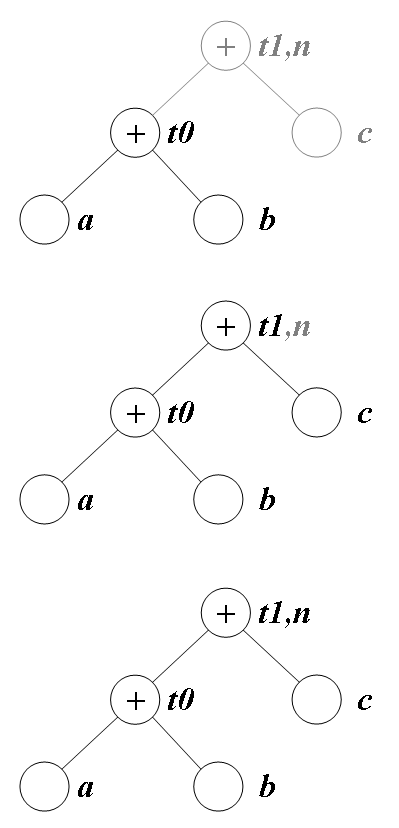
\includegraphics[width=0.468\linewidth,height=1.0\linewidth]{opt001.png}
%%\end{htmlonly}
%%\begin{latexonly}
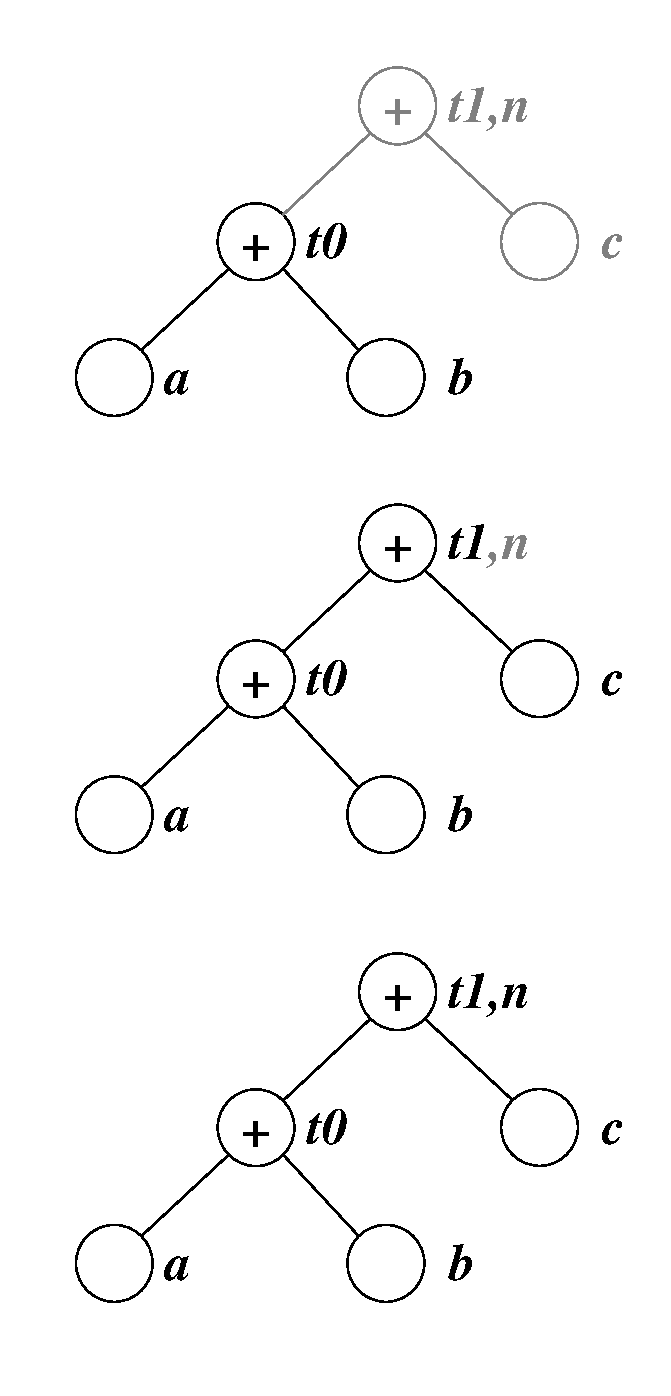
\includegraphics[width=0.468\linewidth,height=1.0\linewidth]{opt001.eps}
%%\end{latexonly}
\caption{{\em dag} of example \ref{optimize_e007}}
\label{optimize_e008}
\end{center}
\end{figure}
Function `{\tt{f}}' is consist of one basic block, and 
`{\tt{n}}' is alive in an exit of this basic block.
For the node whose identifier list is `{\tt{t1, n}}',
chose `{\tt{n}}' at \ref{optimize_e054} of {\bf Assignment judge algorithm}.
After appling algorithms of this section,
3 address codes become like bellow.
\begin{verbatim}
f:
  t0 := a + b
   n := t0 + c
\end{verbatim}
\end{Example}

\begin{Example}
\label{optimize_e009}
\begin{verbatim}
int f(void){ int n = 2; return n + 3; }
\end{verbatim}
3 address codes become like bellow.
\begin{verbatim}
f:
   n := 2
  t0 := n + 3
   return t0
\end{verbatim}
Figure \ref{optimize_e010} illustrates the process of creating
{\em dag} from these 3 address codes.
\begin{figure}[htbp]
\begin{center}
%%\begin{htmlonly}
%%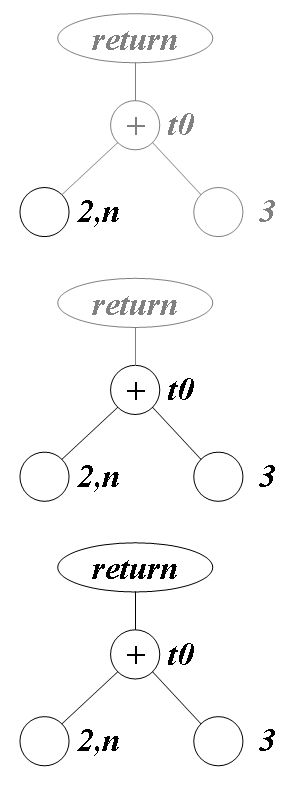
\includegraphics[width=0.392\linewidth,height=1.0\linewidth]{opt002.png}
%%\end{htmlonly}
%%\begin{latexonly}
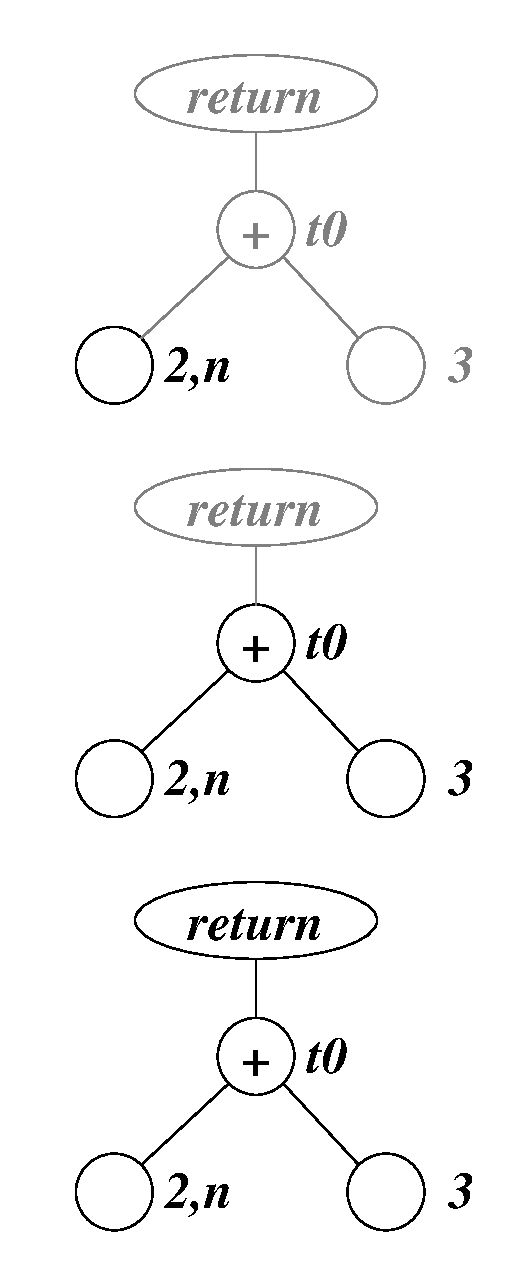
\includegraphics[width=0.392\linewidth,height=1.0\linewidth]{opt002.eps}
%%\end{latexonly}
\caption{{\em dag} of example \ref{optimize_e009}}
\label{optimize_e010}
\end{center}
\end{figure}
Function `{\tt{f}}' is consist of one basic block, and 
`{\tt{2, 3}}' are alive in an exit of this basic block.
For the node whose identifier list is `{\tt{2, n}}',
chose `{\tt{2}}' at \ref{optimize_e055} of {\bf Assignment judge algorithm}.
After appling algorithms of this section,
3 address codes become like bellow.
\begin{verbatim}
f:
  t0 := 2 + 3
   return t0
\end{verbatim}
This example shows that
compile-time evaluationable 3 address code may be generated
after appling algorithms of this section. But in this section,
no more discussion.
\end{Example}

\begin{Example}
\label{optimize_e011}
\begin{verbatim}
int n; void g(void); void f(void){ n = 2; g(); ++n; }
\end{verbatim}
3 address codes become like bellow.
\begin{verbatim}
f:
   n := 2
  t0 := 2
   call g
   n := n + 1
  t1 := n
\end{verbatim}
Figure \ref{optimize_e012} illustrates the process of creating
{\em dag} at the point that {\tt{call g}} is processed.

\begin{figure}[htbp]
\begin{center}
%%\begin{htmlonly}
%%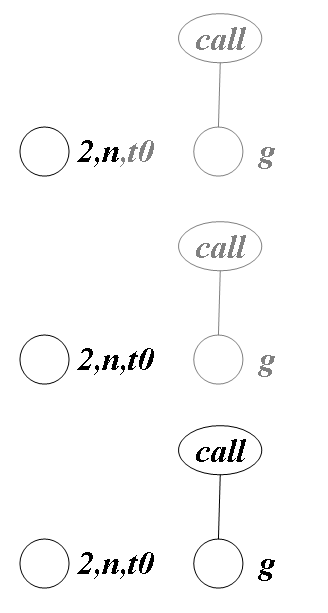
\includegraphics[width=0.530\linewidth,height=1.0\linewidth]{opt003.png}
%%\end{htmlonly}
%%\begin{latexonly}
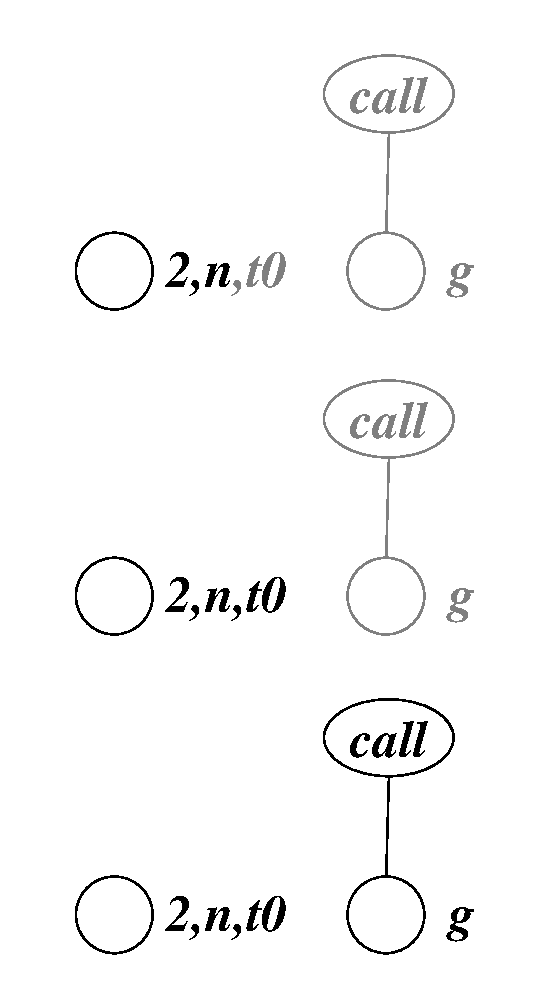
\includegraphics[width=0.530\linewidth,height=1.0\linewidth]{opt003.eps}
%%\end{latexonly}
\caption{{\em dag} of example \ref{optimize_e011}}
\label{optimize_e012}
\end{center}
\end{figure}
Function `{\tt{f}}' is consist of one basic block, and 
`{\tt{n, g, 1, 2}}' are alive in an exit of this basic block.
At \ref{optimize_e112} of {\bf Creation {\em dag} of basic block algorithm},
for {\tt{call g}},
{\bf Code generation algorithm from {\em dag}} is applied.
For the node whose identifier list is `{\tt{2, n, t0}}',
chose `{\tt{2}}'
at \ref{optimize_e055} of {\bf Assignment judge algorithm}.
{\tt{n := 2}} is generated, but for `{\tt{t0}}', 
assignment isn't generated. 
After appling algorithms of this section,
This {\em dag} is converted to like bellow.
\begin{verbatim}
   n := 2
   call g
\end{verbatim}
\end{Example}

\begin{Example}
\label{optimize_e013}
\begin{verbatim}
int n; void f(int* p){ n = 2; *p = 3; ++n; }
\end{verbatim}
3 address codes become like bellow.
\begin{verbatim}
f:
   n := 2
  t0 := 2
  t1 := p
 *t1 := 3
  t2 := 3
   n := n + 1
  t3 := n
\end{verbatim}
Figure \ref{optimize_e014} illustrates the process of creating
{\em dag} at the point that {\tt{*t1 := 3}} is processed.
\begin{figure}[htbp]
\begin{center}
%%\begin{htmlonly}
%%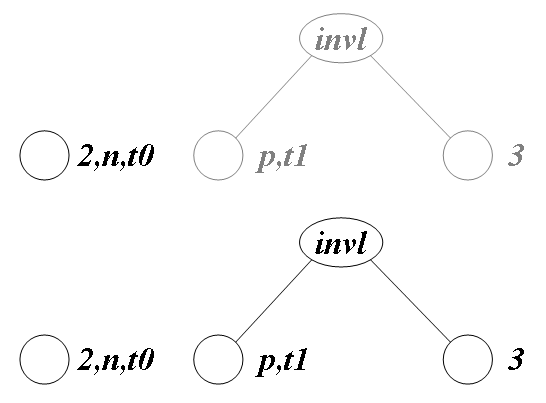
\includegraphics[width=1.0\linewidth,height=0.729\linewidth]{opt004.png}
%%\end{htmlonly}
%%\begin{latexonly}
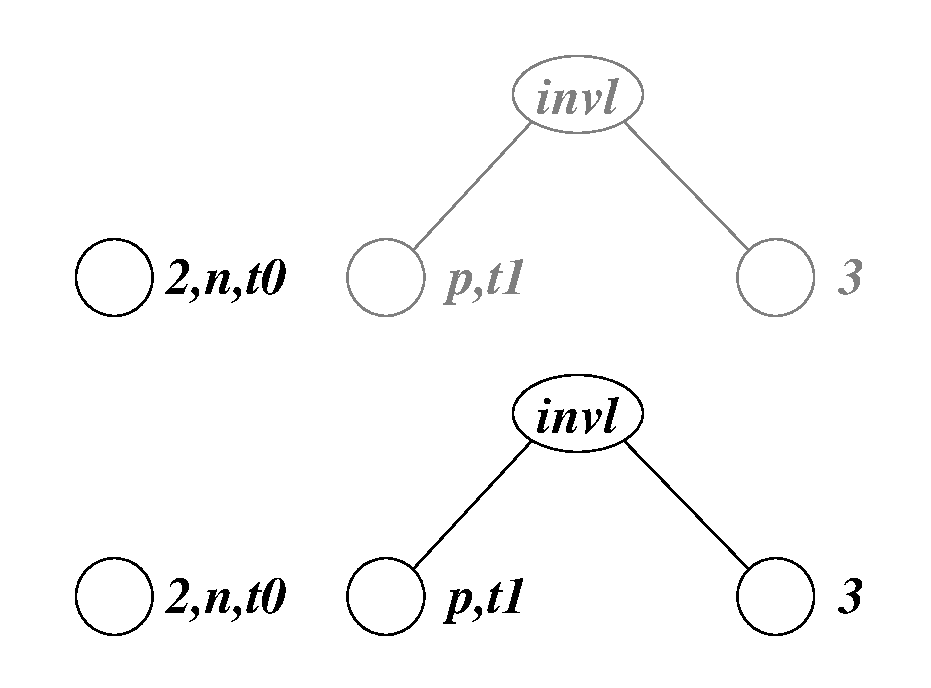
\includegraphics[width=1.0\linewidth,height=0.729\linewidth]{opt004.eps}
%%\end{latexonly}
\caption{{\em dag} of example \ref{optimize_e013}}
\label{optimize_e014}
\end{center}
\end{figure}

Function `{\tt{f}}' is consist of one basic block, and 
`{\tt{n, 1, 2, 3}}' are alive in an exit of this basic block.
At \ref{optimize_e112} of {\bf Creation {\em dag} of basic block algorithm},
for {\tt{*t1 := 3}},
{\bf Code generation algorithm from {\em dag}} is applied.
For the node whose identifier list is `{\tt{2, n, t0}}',
chose `{\tt{2}}'
at \ref{optimize_e055} of {\bf Assignment judge algorithm}.
{\tt{n := 2}} is generated, but for `{\tt{t0}}', 
assignment isn't generated.
For the node whose identifier list is `{\tt{p, t1}}',
chose `{\tt{p}}'
at \ref{optimize_e055} of {\bf Assignment judge algorithm}.
For `{\tt{t0}}', 
assignment isn't generated. 
After appling algorithms of this section,
this dag is converted to like bellow.
\begin{verbatim}
   n := 2
  *p := 3
\end{verbatim}
\end{Example}

\begin{Example}
\label{optimize_e039}
\begin{verbatim}

int f(int a, int b)
{ int c = a, d = b; return (a + b) + (c + d); }
\end{verbatim}
3 address codes become like bellow.
\begin{verbatim}
f:
  t0 := a
   c := t0
  t1 := b
   d := t1
  t2 := a + b
  t3 := c + d
  t4 := t2 + t3
  return t4
\end{verbatim}
Figure \ref{optimize_e040} shows {\em dag} for these 3 address codes.
\begin{figure}[htbp]
\begin{center}
%%\begin{htmlonly}
%%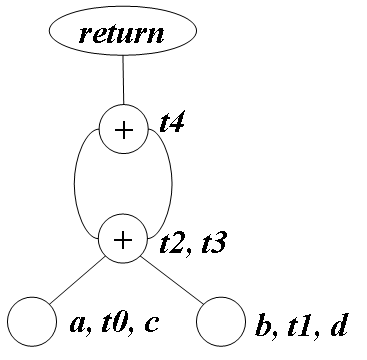
\includegraphics[width=0.724\linewidth,height=0.7\linewidth]{opt021.png}
%%\end{htmlonly}
%%\begin{latexonly}
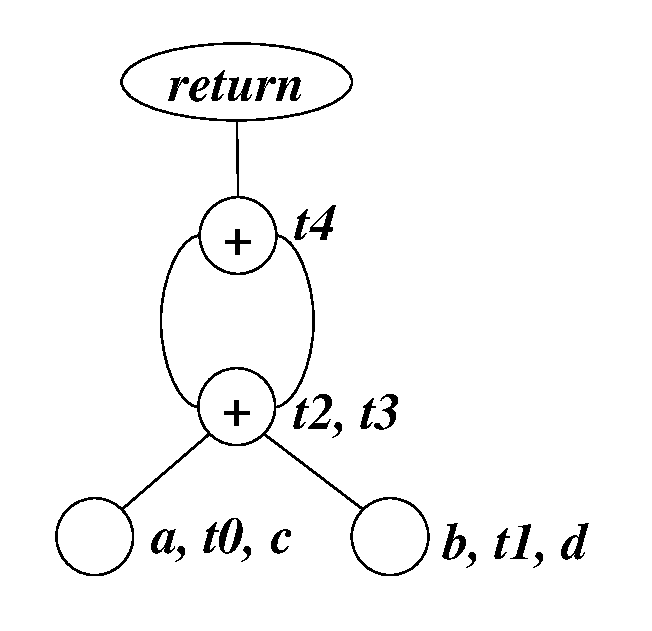
\includegraphics[width=0.724\linewidth,height=0.7\linewidth]{opt021.eps}
%%\end{latexonly}
\caption{{\em dag} of example \ref{optimize_e039}}
\label{optimize_e040}
\end{center}
\end{figure}
For the node whose identifier list is `{\tt{a, t0, c}}',
chose `{\tt{a}}' at \ref{optimize_e055} of {\bf Assignment judge algorithm}.
Assignment is not generated for `{\tt{t0, c}}'.
Simillary, for the node whose identifier list is `{\tt{b, t1, d}}',
chose `{\tt{b}}' at \ref{optimize_e055}
of {\bf Assignment judge algorithm} and
assignment is not generated for `{\tt{t1, d}}'.
For the node whose identifier list is `{\tt{t2, t3}}',
chose `{\tt{t2}}' at \ref{optimize_e054}
of {\bf Assignment judge algorithm}.
After appling algorithms of this section,
3 address codes become like bellow.
\begin{verbatim}
f:
  t2 := a + b
  t4 := t2 + t2
  return t4
\end{verbatim}
\end{Example}

\begin{Example}
\label{optimize_e041}
\begin{verbatim}

int f(int a, int b, int c, int d, int e)
{ return (a+b+(a+b-c)*(d+e))*((a+b-c)*(d+e)-e); }
\end{verbatim}
3 address codes become like bellow.
\begin{verbatim}
f:
  t0 := a + b
  t1 := a + b
  t2 := t1 - c
  t3 := d + e
  t4 := t2 * t3
  t5 := t0 + t4
  t6 := a + b
  t7 := t6 - c
  t8 := d + e
  t9 := t7 * t8
  t10 := t9 - e
  t11 := t5 * t10
  return t11
\end{verbatim}
Figure \ref{optimize_e042} shows {\em dag} for these 3 address codes.
\begin{figure}[htbp]
\begin{center}
%%\begin{htmlonly}
%%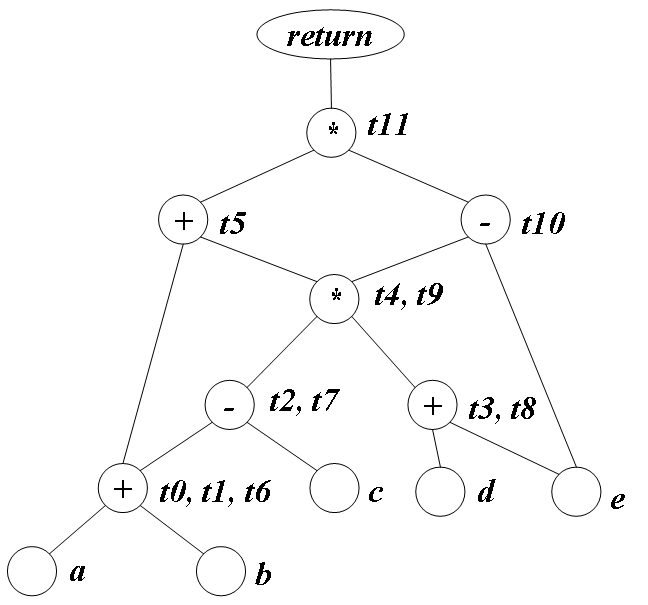
\includegraphics[width=1.051\linewidth,height=1.0\linewidth]{opt022.png}
%%\end{htmlonly}
%%\begin{latexonly}
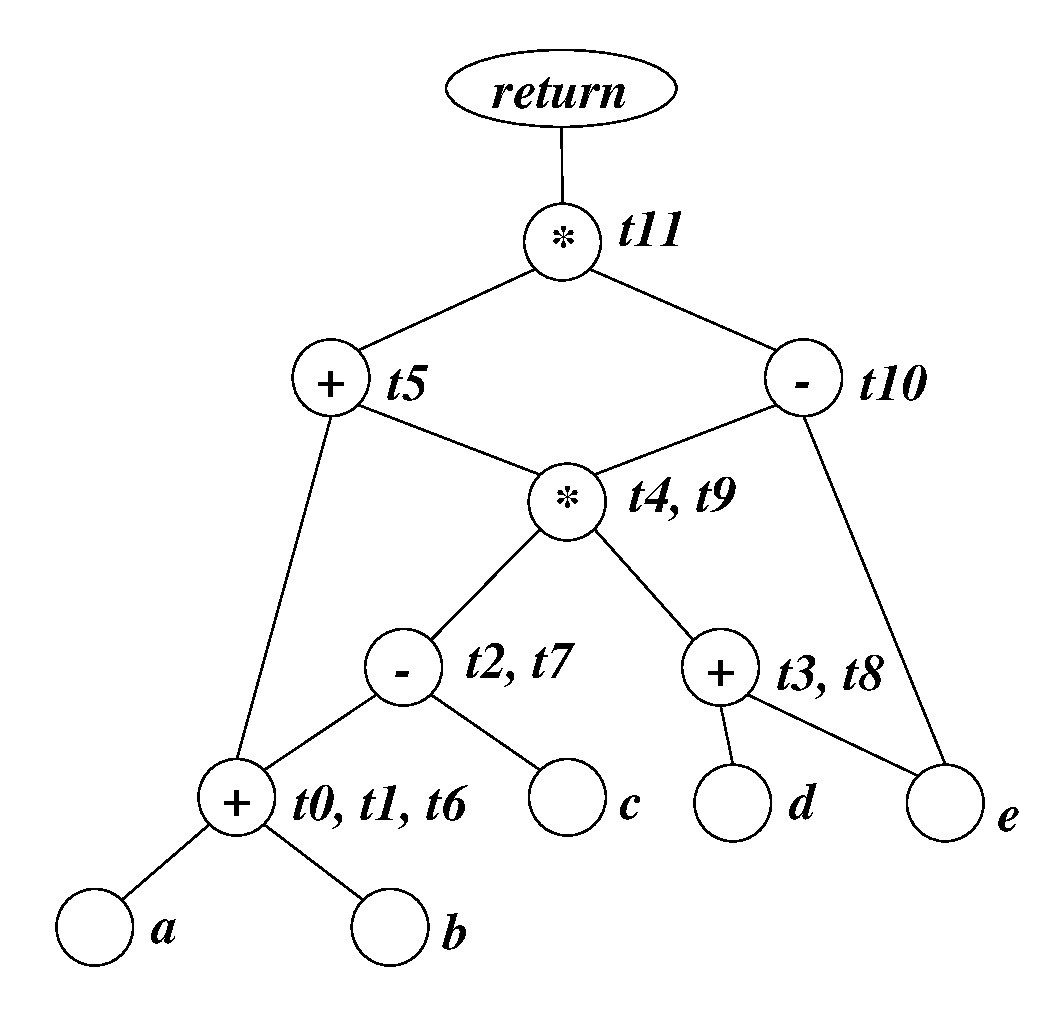
\includegraphics[width=1.051\linewidth,height=1.0\linewidth]{opt022.eps}
%%\end{latexonly}
\caption{{\em dag} of example \ref{optimize_e041}}
\label{optimize_e042}
\end{center}
\end{figure}
Function `{\tt{f}}' is consist of one basic block, and 
no identifier is alive in an exit of this basic block.
For the node whose identifier list is `{\tt{t0, t1, t6}}',
chose `{\tt{t0}}' at \ref{optimize_e054}
of {\bf Assignment judge algorithm}.
For the node whose identifier list is `{\tt{t2, t7}}',
chose `{\tt{t2}}' at \ref{optimize_e054}
of {\bf Assignment judge algorithm}.
For the node whose identifier list is `{\tt{t3, t8}}',
chose `{\tt{t3}}' at \ref{optimize_e054}
of {\bf Assignment judge algorithm}.
For the node whose identifier list is `{\tt{t4, t9}}',
chose `{\tt{t3}}' at \ref{optimize_e054}
of {\bf Assignment judge algorithm}.
After appling algorithms of this section,
3 address codes become like bellow.
\begin{verbatim}
f:
  t0 := a + b
  t2 := t0 - c
  t3 := d + e
  t4 := t2 * t3
  t5 := t0 + t4
  t10 := t4 - e
  t11 := t5 * t10
  return t11
\end{verbatim}
\end{Example}

\begin{Example}
\label{optimize_e043}
\begin{verbatim}

int x, y;
void f(int b){ int a = b + x; b = a - y; x = b + x; y = a - y; }
\end{verbatim}
3 address codes become like bellow.
\begin{verbatim}
f:
  t0 := b + x
   a := t0
  t1 := a - y
   b := t1
  t2 := b + x
   x := t2
  t3 := a - y
   y := t3
\end{verbatim}
Figure \ref{optimize_e044} shows {\em dag} for these 3 address codes.
\begin{figure}[htbp]
\begin{center}
%%\begin{htmlonly}
%%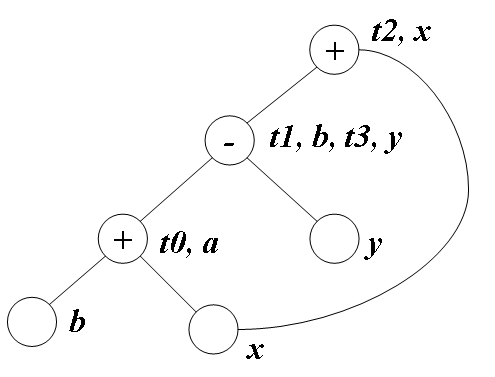
\includegraphics[width=0.7\linewidth,height=0.540\linewidth]{opt023.png}
%%\end{htmlonly}
%%\begin{latexonly}
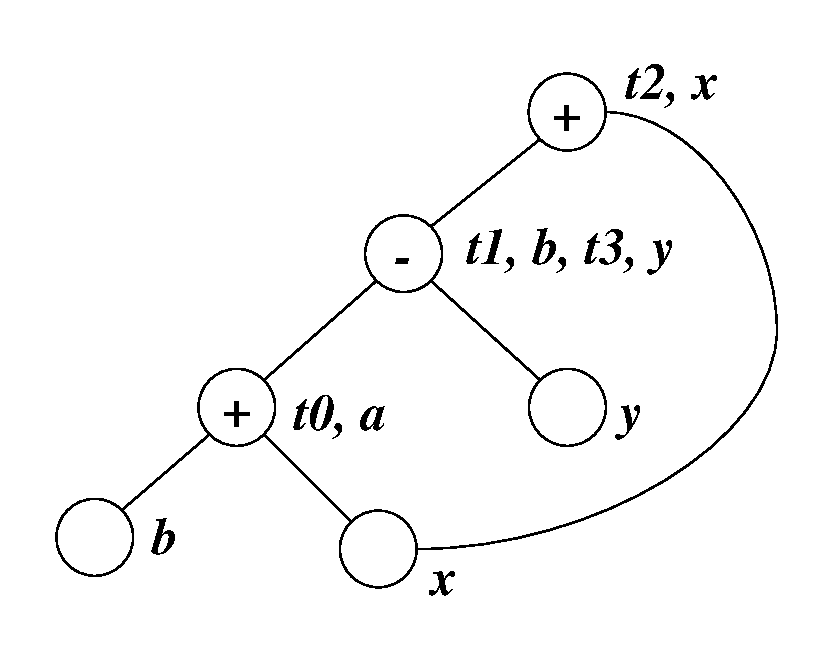
\includegraphics[width=0.7\linewidth,height=0.540\linewidth]{opt023.eps}
%%\end{latexonly}
\caption{{\em dag} of example \ref{optimize_e043}}
\label{optimize_e044}
\end{center}
\end{figure}
Function `{\tt{f}}' is consist of one basic block, and 
`{\tt{x, y}}' are alive in an exit of this basic block.
For the node whose identifier list is `{\tt{t0, a}}',
chose `{\tt{t0}}' at \ref{optimize_e054} of {\bf Assignment judge algorithm}.
For the node whose identifier list is `{\tt{t1, b, t3, y}}',
chose `{\tt{y}}' at \ref{optimize_e054} of {\bf Assignment judge algorithm}.
For the node whose identifier list is `{\tt{t2, y}}',
chose `{\tt{y}}' at \ref{optimize_e054} of {\bf Assignment judge algorithm}.
After appling algorithms of this section,
3 address codes become like bellow.
\begin{verbatim}
f:
  t0 := b + x
  y := t0 - y
  x := y + x
\end{verbatim}
\end{Example}

\begin{Example}
\label{optimize_e045}
\begin{verbatim}

int x, y;
void f(int a, int b, int c){ x = a + b; a = a - c; b = b + c; y = a + b; }
\end{verbatim}
3 address codes become like bellow.
\begin{verbatim}
f:
  t0 := a + b
   x := t0
  t1 := a - c
   a := t1
  t2 := b + c
   b := t2
  t3 := a + b
   y := t3
\end{verbatim}
Figure \ref{optimize_e046} shows {\em dag} for these 3 address codes.
\begin{figure}[htbp]
\begin{center}
%%\begin{htmlonly}
%%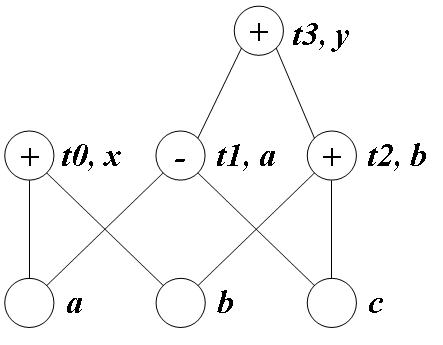
\includegraphics[width=0.7\linewidth,height=0.540\linewidth]{opt024.png}
%%\end{htmlonly}
%%\begin{latexonly}
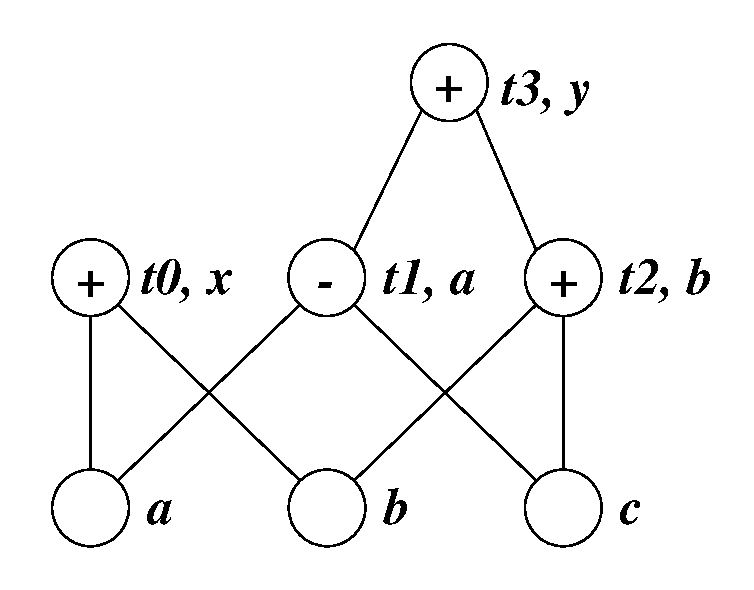
\includegraphics[width=0.7\linewidth,height=0.540\linewidth]{opt024.eps}
%%\end{latexonly}
\caption{{\em dag} of example \ref{optimize_e045}}
\label{optimize_e046}
\end{center}
\end{figure}
Function `{\tt{f}}' is consist of one basic block, and 
`{\tt{x, y}}' are alive in an exit of this basic block.
For the node whose identifier list is `{\tt{t0, x}}',
chose `{\tt{x}}' at \ref{optimize_e054} of {\bf Assignment judge algorithm}.
For the node whose identifier list is `{\tt{t1, a}}',
chose `{\tt{t1}}' at \ref{optimize_e054} of {\bf Assignment judge algorithm}.
For the node whose identifier list is `{\tt{t2, b}}',
chose `{\tt{t2}}' at \ref{optimize_e054} of {\bf Assignment judge algorithm}.
For the node whose identifier list is `{\tt{t3, y}}',
chose `{\tt{y}}' at \ref{optimize_e054} of {\bf Assignment judge algorithm}.
After appling algorithms of this section,
3 address codes become like bellow.
\begin{verbatim}
f:
   x := a + b
  t1 := a - c
  t2 := b + c
   y := t1 + t2
\end{verbatim}
\end{Example}

\begin{Example}
\label{optimize_e015}
\begin{verbatim}
int a, b, c, d; void f(void){ (a = b) + (c = d); }
\end{verbatim}
3 address codes become like bellow.
\begin{verbatim}
f:
  t0 := b
   a := t0
  t1 := d
   c := t1
  t2 := t0 + t1
\end{verbatim}
Figure \ref{optimize_e016} shows {\em dag} for these 3 address codes.
\begin{figure}[htbp]
\begin{center}
%%\begin{htmlonly}
%%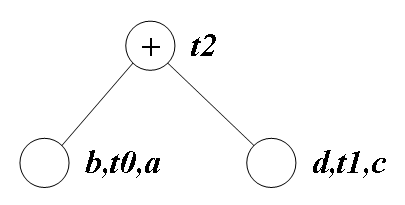
\includegraphics[width=0.7\linewidth,height=0.362\linewidth]{opt005.png}
%%\end{htmlonly}
%%\begin{latexonly}
\includegraphics[width=0.7\linewidth,height=0.362\linewidth]{opt005.eps}
%%\end{latexonly}
\caption{{\em dag} of example \ref{optimize_e015}}
\label{optimize_e016}
\end{center}
\end{figure}
Function `{\tt{f}}' is consist of one basic block, and 
`{\tt{a, b, c, d}}' are alive in an exit of this basic block.
For the node whose identifier list is `{\tt{b, t0, a}}',
chose `{\tt{b}}' at \ref{optimize_e055} of {\bf Assignment judge
 algorithm}. For `{\tt{t0}}', assignment is not generated.
But for `{\tt{a}}', generate {\tt{a := b}}.
Simillary, for the node whose identifier list is `{\tt{d, t1, c}}',
chose `{\tt{d}}' at \ref{optimize_e055} of {\bf Assignment judge
 algorithm}. For `{\tt{t1}}', assignment is not generated.
But for `{\tt{d}}', generate {\tt{c := d}}.
For the node whose identifier list is `{\tt{t2}}',
3 address code {\tt{t2 := a + c}} is not generated
at \ref{optimize_e056} of {\bf Code generation algorithm from {\em dag}}
because `{\tt{t2}}' is not alive in an exit of this basic block.
After appling algorithms of this section,
3 address codes become like bellow.
\begin{verbatim}
f:
  a := b
  c := d
\end{verbatim}
\end{Example}

\begin{Example}
\begin{verbatim}
int g(void); void f(void){ g(); }
\end{verbatim}
3 address codes become like bellow.
\begin{verbatim}
f:
  t0 := call g
\end{verbatim}
Function `{\tt{f}}' is consist of one basic block.
Because `{\tt{t0}}' is not alive in an exit of this basic block,
{\tt{t0 := call g}} is converted to {\tt{call g}} at
\ref{optimize_e057} of {\bf Code generation algorithm from {\em dag}}.
\end{Example}

\begin{Example}
\label{optimize_e017}
\begin{verbatim}

int g(int);
void f(void){ int n = 2; int* p = &n; *p = 1; g(*p); }
\end{verbatim}
3 address codes become like bellow.
\begin{verbatim}
f:
   n := 2
  t0 := &n
   p := t0
  t1 := p
 *t1 := 1
  t2 := 1
  t3 := p
  t4 := *t3
  param t4
  t5 := call g
\end{verbatim}
Figure \ref{optimize_e018} shows {\em dag} at the point that
{\tt{*t1 := 1}} is processed.
\begin{figure}[htbp]
\begin{center}
%%\begin{htmlonly}
%%\includegraphics[width=0.8\linewidth,height=0.525\linewidth]{opt007.png}
%%\end{htmlonly}
%%\begin{latexonly}
\includegraphics[width=0.8\linewidth,height=0.525\linewidth]{opt007.eps}
%%\end{latexonly}
\caption{{\em dag} of example \ref{optimize_e017}}
\label{optimize_e018}
\end{center}
\end{figure}
Function `{\tt{f}}' is consist of one basic block, and 
`{\tt{g, 1, 2}}' are alive in an exit of this basic block.
For the node whose identifier list is `{\tt{2, n}}',
chose `{\tt{2}}' at \ref{optimize_e055} of {\bf Assignment judge algorithm}.
`{\tt{n}}' is not alive in an exit of this basic block, but
the condition \ref{optimize_e052} of {\bf Assignment judge algorithm}
holds true, so generate {\tt{n := 2}} and return {\tt{n}} from
{\bf Assignment judge algorithm}.
For the node whose identifier list is `{\tt{t0, p, t1}}',
chose `{\tt{p}}' at \ref{optimize_e054} of {\bf Assignment judge
 algorithm} because `{\tt{p}}' is used later.
 `{\tt{t1}}' is not alive in an exit of this basic block,
assignment is not generated.
After appling algorithms of this section,
this {\em dag} is converted to like bellow.
\begin{verbatim}
  n := 2
  p := &n
 *p := 1
\end{verbatim}
The best codes for `{\tt{f}}' are
\begin{verbatim}
f:
  param 1
  call g
\end{verbatim}
But in this section, no more discussion for the best codes.
\end{Example}

\begin{Example}
\label{optimize_e023}
\begin{verbatim}
int f(void){ int n = 2; int* p = &n; *p = 1; return *p; }
\end{verbatim}
3 address codes become like bellow.
\begin{verbatim}
f:
   n := 2
  t0 := &n
   p := t0
  t1 := p
 *t1 := 1
  t2 := 1
  t3 := p
  t4 := *t3
  return t4
\end{verbatim}
Figure \ref{optimize_e024} shows {\em dag} at the point
that {\tt{*t1 := 1}} is processed.
\begin{figure}[htbp]
\begin{center}
%%\begin{htmlonly}
%%\includegraphics[width=0.7\linewidth,height=0.423\linewidth]{opt010.png}
%%\end{htmlonly}
%%\begin{latexonly}
\includegraphics[width=0.7\linewidth,height=0.423\linewidth]{opt010.eps}
%%\end{latexonly}
\caption{{\em dag} of example \ref{optimize_e023}}
\label{optimize_e024}
\end{center}
\end{figure}
Function `{\tt{f}}' is consist of one basic block, and 
`{\tt{1, 2}}' is alive in an exit of this basic block.
For the node whose identifier list is `{\tt{2, n}}',
chose `{\tt{2}}' at \ref{optimize_e055} of {\bf Assignment judge algorithm}.
`{\tt{n}}' is not alive in an exit of this basic block,
but {\tt{n := 2}} is generated becase of \ref{optimize_e052}
of {\bf Assignment judge algorithm}. And return `{\tt{n}}'
form {\bf Assignment judge algorithm}.
For the node whose identifier list is `{\tt{t0, p, t1}}',
chose `{\tt{p}}' at \ref{optimize_e054} of {\bf Assignment judge
 algorithm} because `{\tt{p}}' is used later.
`{\tt{t1}}' is not alive in an exit of this basic block,
so assignment is not genearted.
After appling algorithms of this section,
3 address codes become like bellow.
\begin{verbatim}
  n := 2
  p := &n
 *p := 1
\end{verbatim}
The best codes for `{\tt{f}}' are
\begin{verbatim}
f:
  return 1
\end{verbatim}
But in this section, no more discussion for the best codes.
\end{Example}

\begin{Example}
\label{optimize_e019}
\begin{verbatim}
int g(int); void f(void){ int n = 2; int* p = &n; g(*p); }
\end{verbatim}
3 address codes become like bellow.
\begin{verbatim}
f:
   n := 2
  t0 := &n
   p := t0
  t1 := p
  t2 := *t1
  param t2
  t3 := call g
\end{verbatim}
Figure \ref{optimize_e020} shows {\em dag} for these 3 address codes.
\begin{figure}[htbp]
\begin{center}
%%\begin{htmlonly}
%%\includegraphics[width=1.0\linewidth,height=0.507\linewidth]{opt008.png}
%%\end{htmlonly}
%%\begin{latexonly}
\includegraphics[width=1.0\linewidth,height=0.507\linewidth]{opt008.eps}
%%\end{latexonly}
\caption{{\em dag} of example \ref{optimize_e019}}
\label{optimize_e020}
\end{center}
\end{figure}
Function `{\tt{f}}' is consist of one basic block, and 
`{\tt{g, 2}}' are alive in an exit of this basic block.
For the node whose identifier list is `{\tt{t2, n}}',
chose `{\tt{2}}' at \ref{optimize_e055} of {\bf Assignment judge algorithm}.
`{\tt{n}}' is not alive in an exit of this block,
but {\tt{n := 2}} is generated becase of \ref{optimize_e052}
of {\bf Assignment judge algorithm}. And return `{\tt{n}}'
For the node whose identifier list is `{\tt{t0, p, t1}}',
chose `{\tt{t0}}' at \ref{optimize_e054} of {\bf Assignment judge algorithm}.
After appling algorithms of this section,
3 address codes become like bellow.
\begin{verbatim}
f:
   n := 2
  t0 := &n
  t2 := *t0
  param t2
  call g
\end{verbatim}
The best codes for `{\tt{f}}' are
\begin{verbatim}
f:
  param 2
  call g
\end{verbatim}
But in this section, no more discussion for the best codes.
\end{Example}

\begin{Example}
\label{optimize_e021}
\begin{verbatim}
void g(int, int); void f(int x){ g(x+1,x+2); }
\end{verbatim}
3 address codes become like bellow.
\begin{verbatim}
f:
  t0 := x + 1
  t1 := x + 2
  param t0
  param t1
  call g
\end{verbatim}
Figure \ref{optimize_e022} shows {\em dag} for these 3 address codes.
\begin{figure}[htbp]
\begin{center}
%%\begin{htmlonly}
%%\includegraphics[width=0.8\linewidth,height=0.470\linewidth]{opt009.png}
%%\end{htmlonly}
%%\begin{latexonly}
\includegraphics[width=0.8\linewidth,height=0.470\linewidth]{opt009.eps}
%%\end{latexonly}
\caption{{\em dag} of example \ref{optimize_e021}}
\label{optimize_e022}
\end{center}
\end{figure}
Similary so far, applying {\bf Code generation algorithm from {\em
 dag}}, and get the same 3 address codes.
As we described at \ref{_3ac_e000}, frontend must 
generate {\tt{param}} or {\tt{param}}s continually
which is or are referenced by {\tt{call}}, just before generating
{\tt{call}}, and the constraint is kept after optimization.
\end{Example}

\begin{Example}
\label{optimize_e025}
\begin{verbatim}
void f(int* p){ --*p; }
\end{verbatim}
3 address codes become like bellow.
\begin{verbatim}
f:
  t0 := p
  t1 := *t0
  t1 := t1 - 1
 *t0 := t1
\end{verbatim}
Figure \ref{optimize_e026} shows {\em dag} for these 3 address codes.
\begin{figure}[htbp]
\begin{center}
%%\begin{htmlonly}
%%\includegraphics[width=0.7\linewidth,height=0.552\linewidth]{opt011.png}
%%\end{htmlonly}
%%\begin{latexonly}
\includegraphics[width=0.7\linewidth,height=0.552\linewidth]{opt011.eps}
%%\end{latexonly}
\caption{{\em dag} of example \ref{optimize_e025}}
\label{optimize_e026}
\end{center}
\end{figure}
Function `{\tt{f}}' is consist of one basic block, and 
`{\tt{1}}' is alive in an exit of this basic block.
For the node whose identifier list is `{\tt{p, t0}}',
chose `{\tt{p}}' at \ref{optimize_e055} of {\bf Assignment judge
 algorithm}.
`{\tt{t0}}' is not alive in an exit of this basic block, so
assignment is not generated.
After appling algorithms of this section,
3 address codes become like bellow.
\begin{verbatim}
f:
  t1 := *p
  t1 := t1 - 1
  *p := t1
\end{verbatim}
\end{Example}

\begin{Example}
\label{optimize_e027}
\begin{verbatim}
void g(double, int, int);
void f(double d){ int a = (int)d; int b = a; g(d,a,b); }
\end{verbatim}
3 address codes become like bellow.
\begin{verbatim}
f:
  t0 := (int)d
   a := t0
  t1 := a
   b := t1
  t2 := d
  t3 := a
  t4 := b
  param t2
  param t3
  param t4
  call g
\end{verbatim}
Figure \ref{optimize_e028} shows {\em dag} for these 3 address codes.
\begin{figure}[htbp]
\begin{center}
%%\begin{htmlonly}
%%\includegraphics[width=1.0\linewidth,height=0.483\linewidth]{opt012.png}
%%\end{htmlonly}
%%\begin{latexonly}
\includegraphics[width=1.0\linewidth,height=0.483\linewidth]{opt012.eps}
%%\end{latexonly}
\caption{{\em dag} of example \ref{optimize_e027}}
\label{optimize_e028}
\end{center}
\end{figure}
Function `{\tt{f}}' is consist of one basic block, and 
`{\tt{g}}' is alive in an exit of this basic block.
For the node whose identifier list is `{\tt{d, t2}}',
chose `{\tt{d}}' at \ref{optimize_e055} of {\bf Assignment judge
 algorithm}.
`{\tt{t2}}' is not alive in an exit of this basic block, so
assignment is not generated.
For the node whose identifier list is `{\tt{t0, a, t1, b, t3, t4}}',
chose `{\tt{t0}}' at \ref{optimize_e054} of {\bf Assignment judge
 algorithm}.
`{\tt{a, t1, b, t3, t4}}' are not alive in an exit of this basic block, so
assignments are not generated.
After appling algorithms of this section,
3 address codes become like bellow.
\begin{verbatim}
f:
  t0 := (int)d
  param d
  param t0
  param t0
  call g
\end{verbatim}
\end{Example}

\begin{Example}
\label{optimize_e029}
\begin{verbatim}
int n; int g(int); void f(void){ n = 2; n = g(3); ++n; }
\end{verbatim}
3 address codes become like bellow.
\begin{verbatim}
f:
   n := 2
  t0 := 2
  param 3
  t1 := call g
   n := t1
   n := n + 1
  t2 := n
\end{verbatim}
Figure \ref{optimize_e030} shows {\em dag} for these 3 address codes.
Here, the upper of figure \ref{optimize_e030} is {\em dag}
at the point that {\tt{t1 := call g}} is processed.
\begin{figure}[htbp]
\begin{center}
%%\begin{htmlonly}
%%\includegraphics[width=0.8\linewidth,height=0.571\linewidth]{opt013.png}
%%\end{htmlonly}
%%\begin{latexonly}
\includegraphics[width=0.8\linewidth,height=0.571\linewidth]{opt013.eps}
%%\end{latexonly}
\caption{{\em dag} of example \ref{optimize_e029}}
\label{optimize_e030}
\end{center}
\end{figure}
Function `{\tt{f}}' is consist of one basic block.
`{\tt{g, n, 1, 2, 3}}' are alive in an exit of the this basic block.

For the node whose identifier list is `{\tt{2, n, t0}}',
chose `{\tt{2}}' at \ref{optimize_e054} of {\bf Assignment judge
 algorithm}.
`{\tt{n}}' is alive in an exit of this basic block, so
{\tt{n := 2}} is generated. But
`{\tt{t0}}' is not alive in an exit of this basic block, so
assignment is not generated.
The upper {\em dag} of the figure \ref{optimize_e030} 
is converted to like bellow.
\begin{verbatim}
   n := 2
  pamar 3
  t1 := call g
\end{verbatim}
For the node whose identifier list is `{\tt{t1, n}}',
chose `{\tt{t1}}' at \ref{optimize_e054} of {\bf Assignment judge
 algorithm}.
`{\tt{n}}' is alive in an exit of this basic block, but
assignment is not generated because {\tt{node[n]}} is
not equalt to this node.
For the node whose identifier list is `{\tt{n, t2}}',
`{\tt{t2}}' is not alive in an exit of this basic block, 
so assignment is not generated.
The lower {\em dag} of the figure \ref{optimize_e030} 
is converted to like bellow.
\begin{verbatim}
   n := t1 + 1
\end{verbatim}
Finally, 3 address codes becomes like bellow.
\begin{verbatim}
f:
   n := 2
  pamar 3
  t1 := call g
   n := t1 + 1
\end{verbatim}
\end{Example}

\begin{Example}
\label{optimize_e031}
\begin{verbatim}
void g(char*); void f(void){ char s[] = "abc"; g(s); }
\end{verbatim}
3 address codes become like bellow.
\begin{verbatim}
f:
    t0 := &"abc"
  s[0] := 'a'
  s[1] := 'b'
  s[2] := 'c'
  s[3] := '\0'
    t1 := &s
    t2 := t1
    param t2
    call g
\end{verbatim}
Figure \ref{optimize_e032} shows {\em dag} for these 3 address codes.
\begin{figure}[htbp]
\begin{center}
%%\begin{htmlonly}
%%\includegraphics[width=0.859\linewidth,height=1.0\linewidth]{opt016.png}
%%\end{htmlonly}
%%\begin{latexonly}
%\includegraphics[width=0.859\linewidth,height=1.0\linewidth]{opt016.eps}
\includegraphics[width=1.0\linewidth,height=1.2\linewidth]{opt016.eps}
%%\end{latexonly}
\caption{{\em dag} of example \ref{optimize_e031}}
\label{optimize_e032}
\end{center}
\end{figure}
Function `{\tt{f}}' is consist of one basic block, and 
`{\tt{g, "abc", 0, 1, 2, 3, 'a', 'b', 'c', '\verb|\|0'}}'
are alive in an exit of this basic block.
Here, think about nodes whose label is {\tt{loff}} except for 1st one.
They have 3rd child.
`{\tt{s}}' is not alive in an exit of this basic block,
this 3 address code may be omitted if they don't have 3rd child.
But function `{\tt{g}}' call argument is address of `{\tt{s}}'
and we can easyly know that they cannot be omitted.
At \ref{optimize_e064} of {\bf Code generation algorithm from {\em dag}},
{\tt{x[y] := z}} is treated specially for such a reason.
After appling algorithms of this section,
3 address codes become like bellow.
\begin{verbatim}
f:
  s[0] := 'a'
  s[1] := 'b'
  s[2] := 'c'
  s[3] := '\0'
  t1 := &s
  param t1
  call g
\end{verbatim}
\end{Example}

\begin{Example}
\label{optimize_e033}
\begin{verbatim}
void g(int); void f(void){ int n = 1; n = 2; g(n); }
\end{verbatim}
3 address codes become like bellow.
\begin{verbatim}
f:
   n := 1
   n := 2
  t0 := 2
  t1 := n
  param t1
  call g
\end{verbatim}
Figure \ref{optimize_e034} shows {\em dag} for these 3 address codes.
\begin{figure}[htbp]
\begin{center}
%%\begin{htmlonly}
%%\includegraphics[width=0.8\linewidth,height=0.247\linewidth]{opt018.png}
%%\end{htmlonly}
%%\begin{latexonly}
\includegraphics[width=0.8\linewidth,height=0.247\linewidth]{opt018.eps}
%%\end{latexonly}
\caption{{\em dag} of example \ref{optimize_e033}}
\label{optimize_e034}
\end{center}
\end{figure}
After appling algorithms of this section,
3 address codes become like bellow.
\begin{verbatim}
f:
  param 2
  call g
\end{verbatim}
\end{Example}

\begin{Example}
\label{optimize_e037}
\begin{verbatim}
void g(int*, int*); void f(void){ int i[2]; g(&i[0],&i[1]); }
\end{verbatim}
3 address codes become like bellow.
\begin{verbatim}
f:
  t0 := &i
  t1 := &i
  t1 := t1 + 4
  param t0
  param t1
  call g
\end{verbatim}
Figure \ref{optimize_e038} shows {\em dag} for these 3 address codes.
\begin{figure}[htbp]
\begin{center}
%%\begin{htmlonly}
%%\includegraphics[width=1.0\linewidth,height=0.623\linewidth]{opt020.png}
%%\end{htmlonly}
%%\begin{latexonly}
\includegraphics[width=1.0\linewidth,height=0.623\linewidth]{opt020.eps}
%%\end{latexonly}
\caption{{\em dag} of example \ref{optimize_e037}}
\label{optimize_e038}
\end{center}
\end{figure}
After appling algorithms of this section,
3 address codes become like bellow.
\begin{verbatim}
f:
  t0 := &i
  t1 := t0 + 4
  param t0
  param t1
  call g
\end{verbatim}
\end{Example}

\begin{Example}
\label{optimize_e065}
\begin{verbatim}
int n; void g(int); void f(void){ g(n++); }
\end{verbatim}
3 address codes become like bellow.
\begin{verbatim}
f:
  t0 := n
   n := n + 1
  param t0
  call g
\end{verbatim}
Figure \ref{optimize_e066} shows {\em dag} for these 3 address codes.
\begin{figure}[htbp]
\begin{center}
%%\begin{htmlonly}
%%\includegraphics[width=1.0\linewidth,height=0.328\linewidth]{opt027.png}
%%\end{htmlonly}
%%\begin{latexonly}
\includegraphics[width=1.0\linewidth,height=0.328\linewidth]{opt027.eps}
%%\end{latexonly}
\caption{{\em dag} of example \ref{optimize_e065}}
\label{optimize_e066}
\end{center}
\end{figure}
Applying {\bf Assignment judge
 algorithm} to the node whose identifier list is `{\tt{n, t0}}',
this is in the case
of {\bf Assignment judge algorithm (Special case 1)}
because {\tt{node[n]}} is not equal to this node and
{\tt{node[t0]}} is equal to this node.
As a result, {\tt{t0 := n}} is generated.
Finally, 3 address codes become like bellow.
\begin{verbatim}
f:
  t0 := n
   n := t0 + 1
  param t0
  call g
\end{verbatim}
\end{Example}

\begin{Example}
\label{optimize_e068}
\begin{verbatim}

struct S { unsigned int a : 1; unsigned int b : 2; };
extern struct S s; unsigned int f(void){ return s.a + s.b; }
\end{verbatim}
3 address codes become like bellow.
\begin{verbatim}
f:
  t0 := s[0]
  t1 := t0 & 1
  t2 := s[0]
  t3 := t2 >> 1
  t4 := t3 & 3
  t5 := t1 + t4
  return t5
\end{verbatim}
Figure \ref{optimize_e069} shows {\em dag} for these 3 address codes.
\begin{figure}[htbp]
\begin{center}
%%\begin{htmlonly}
%%\includegraphics[width=0.826\linewidth,height=1.0\linewidth]{opt028.png}
%%\end{htmlonly}
%%\begin{latexonly}
\includegraphics[width=0.826\linewidth,height=1.0\linewidth]{opt028.eps}
%%\end{latexonly}
\caption{{\em dag} of example \ref{optimize_e068}}
\label{optimize_e069}
\end{center}
\end{figure}
Similary so far, frontend can detect common expression {\tt{s[0]}}
by applying {\bf Code generation algorithm from {\em dag}}.
After appling algorithms of this section,
3 address codes become like bellow.
\begin{verbatim}
f:
  t0 := s[0]
  t1 := t0 & 1
  t3 := t0 >> 1
  t4 := t3 & 3
  t5 := t1 + t4
  return t5
\end{verbatim}
\end{Example}

\begin{Example}
\label{optimize_e070}
\begin{verbatim}
int f(void){ static int s; return s++; }
\end{verbatim}
3 address codes become like bellow.
\begin{verbatim}
f:
  t0 := s
   s := s + 1
  return t0
\end{verbatim}
Figure \ref{optimize_e071} shows {\em dag} for these 3 address codes.
\begin{figure}[htbp]
\begin{center}
%%\begin{htmlonly}
%%\includegraphics[width=0.8\linewidth,height=0.347\linewidth]{opt029.png}
%%\end{htmlonly}
%%\begin{latexonly}
\includegraphics[width=0.8\linewidth,height=0.347\linewidth]{opt029.eps}
%%\end{latexonly}
\caption{{\em dag} of example \ref{optimize_e070}}
\label{optimize_e071}
\end{center}
\end{figure}
The node whose identifier list is `{\tt{s, t0}}'
is in case of {\bf Assignment judge algorithm (Special case 1) },
so, {\tt{t0 := s}} is generated and the result of this node
is `{\tt{t0}}' not `{\tt{s}}'.
After appling algorithms of this section,
3 address codes become like bellow.
\begin{verbatim}
f:
  t0 := s
   s := t0 + 1
  return t0
\end{verbatim}
\end{Example}

\begin{Example}
\label{optimize_e073}
\begin{verbatim}

struct S { int m; int n; }; void g(struct S);
void f(void){ struct S x, y = { 1, 2 }; x = y; g(x); }
\end{verbatim}
3 address codes become like bellow.
\begin{verbatim}
f:
  y[0] := 1
  y[4] := 2
    t0 := y
     x := t0
    t1 := x
  param t1
  call g
\end{verbatim}
Figure \ref{optimize_e074} shows {\em dag} for these 3 address codes.
\begin{figure}[htbp]
\begin{center}
%%\begin{htmlonly}
%%\includegraphics[width=1.0\linewidth,height=0.439\linewidth]{opt030.png}
%%\end{htmlonly}
%%\begin{latexonly}
%\includegraphics[width=1.0\linewidth,height=0.439\linewidth]{opt030.eps}
\includegraphics[width=1.2\linewidth,height=1.0\linewidth]{opt030.eps}
%%\end{latexonly}
\caption{{\em dag} of example \ref{optimize_e073}}
\label{optimize_e074}
\end{center}
\end{figure}
Function `{\tt{f}}' is consist of one basic block, and 
`{\tt{g, 0, 1, 2, 4}}' are alive in an exit of this basic block.
Because `{\tt{y}}' is not alive in an exit of this basic block,
it's necessary to have parent of the node whose label is {\tt{y[0] := 1}}
for generating code.
3 address codes become like bellow.
\begin{verbatim}
f:
  y[0] := 1
  y[4] := 2
    t0 := y  # Canbe erased.
     x := y  # But this algorithm cannot erase
    t1 := y  # at present state.
  param y
  call g
\end{verbatim}
\end{Example}

\begin{Example}
\label{optimize_e077}
\begin{verbatim}

void g(int, int*, int*);
void f(void)
{ int a = 0; int b = 1; int c = 2; g(a,&b,&c); ++a; g(a,&b,&c); }
\end{verbatim}
3 address codes become like bellow.
\begin{verbatim}
f:
  a := 0
  b := 1
  c := 2
  t0 := &b
  t1 := &c
  t2 := a
  param t2
  param t0
  param t1
  call g
  a := a + 1
  t3 := a
  t4 := &b
  t5 := &c
  t6 := a
  param t6
  param t4
  param t5
  call g
\end{verbatim}
Figure \ref{optimize_e078} shows {\em dag} for these 3 address codes.
\begin{figure}[htbp]
\begin{center}
%%\begin{htmlonly}
%%\includegraphics[width=1.0\linewidth,height=0.894\linewidth]{opt032.png}
%%\end{htmlonly}
%%\begin{latexonly}
\includegraphics[width=1.0\linewidth,height=0.894\linewidth]{opt032.eps}
%%\end{latexonly}
\caption{{\em dag} of example \ref{optimize_e077}}
\label{optimize_e078}
\end{center}
\end{figure}
Similary so far,
after appling algorithms of this section,
3 address codes become like bellow.
\begin{verbatim}
f:
  a := 0
  b := 1
  c := 2
  t0 := &b
  t1 := &c
  param 0
  param t0
  param t1
  call g
  a := a + 1
  t4 := &b
  t5 := &c
  param a
  param t4
  param t5
  call g
\end{verbatim}
\end{Example}

\begin{Example}
\label{optimize_e079}
\begin{verbatim}

void g(void); struct S { int a; }; void h(struct S);
void f(struct S y){ struct S x = { 1 }; g(); x = y; h(x); }
\end{verbatim}
3 address codes become like bellow.
\begin{verbatim}
f:
  x[0] := 1
  call g
  t0 := y
  x := t0
  t1 := x
  param t1
  call h
\end{verbatim}
Figure \ref{optimize_e080} shows {\em dag} for these 3 address codes.
Here, the upper of figure \ref{optimize_e080} is {\em dag}
at the point that {\tt{call g}} is processed.
\begin{figure}[htbp]
\begin{center}
%%\begin{htmlonly}
%%\includegraphics[width=0.6\linewidth,height=0.6\linewidth]{opt033.png}
%%\end{htmlonly}
%%\begin{latexonly}
\includegraphics[width=0.6\linewidth,height=0.6\linewidth]{opt033.eps}
%%\end{latexonly}
\caption{{\em dag} of example \ref{optimize_e079}}
\label{optimize_e080}
\end{center}
\end{figure}
Function `{\tt{f}}' is consist of one basic block, and 
`{\tt{x}}' is not alive in exit of this basic block.
For this reason, no code is generated
for the node whose label is {\tt{x[0] :=
 1}} in the upper {\em dag} of figure \ref{optimize_e080}.
For the node whose identifier list is `{\tt{y, t0, x, t1}}',
chose `{\tt{y}}' at \ref{optimize_e055} of {\bf Assignment judge
algorithm}, and no assignment is generated for `{\tt{t0, x, t1}}'.
After appling algorithms of this section,
3 address codes become like bellow.
\begin{verbatim}
f:
  call g
  param y
  call h
\end{verbatim}
\end{Example}

\begin{Example}
\label{optimize_e081}
\begin{verbatim}

struct S { int a; }; void g(struct S);
void f(struct S y){ struct S x = { 1 }; g(x); x = y; g(x); }
\end{verbatim}
3 address codes become like bellow.
\begin{verbatim}
f:
  x[0] := 1
  t0 := x
  param t0
  call g
  t1 := y
  x := t1
  t2 := x
  param t2
  call g
\end{verbatim}
Figure \ref{optimize_e082} shows {\em dag} for these 3 address codes.
\begin{figure}[htbp]
\begin{center}
%%\begin{htmlonly}
%%\includegraphics[width=0.493\linewidth,height=0.6\linewidth]{opt034.png}
%%\end{htmlonly}
%%\begin{latexonly}
\includegraphics[width=0.493\linewidth,height=0.6\linewidth]{opt034.eps}
%%\end{latexonly}
\caption{{\em dag} of example \ref{optimize_e081}}
\label{optimize_e082}
\end{center}
\end{figure}
Function `{\tt{f}}' is consist of one basic block.
For the node whose identifier list is `{\tt{y, t1, x, t2}}',
chose `{\tt{y}}' and no assignment is generated for
{\tt{t1, x, t2}} becase they are not alive in an exit
of this basic block.
After appling algorithms of this section,
3 address codes become like bellow.
\begin{verbatim}
f:
  x[0] := 1
  param x
  call g
  param y
  call g
\end{verbatim}
\end{Example}

\begin{Example}
\label{optimize_e083}
\begin{verbatim}
void g(int); int x[3][5]; void f(void){ g(x[2][3]); }
\end{verbatim}
3 address codes become like bellow.
\begin{verbatim}
f:
  t0 := &x
  t1 := t0 + 40
  t2 := x[52]
  param t2
  call g
\end{verbatim}
Figure \ref{optimize_e084} shows {\em dag} for these 3 address codes.
\begin{figure}[htbp]
\begin{center}
%%\begin{htmlonly}
%%\includegraphics[width=1.0\linewidth,height=0.509\linewidth]{opt035.png}
%%\end{htmlonly}
%%\begin{latexonly}
\includegraphics[width=1.0\linewidth,height=0.509\linewidth]{opt035.eps}
%%\end{latexonly}
\caption{{\em dag} of example \ref{optimize_e083}}
\label{optimize_e084}
\end{center}
\end{figure}
Function `{\tt{f}}' is consist of one basic block,
and `{\tt{t0, t1, t2}}' is not alive in an exit of this basic block.
Similary so far, 
after appling algorithms of this section,
3 address codes become like bellow.
\begin{verbatim}
f:
  t0 := &x
  t2 := x[52]
  param t2
  call g
\end{verbatim}
Here, {\tt{t0 := \&x}} can be ommited if 
applying {\bf Creation {\em dag} of basic block algorithm} an
{\bf Code generation algorithm from {\em dag}} again.
\end{Example}

\begin{Example}
\label{optimize_e075}
\begin{verbatim}

extern int a[];
void f(int i, int j){ int x = a[i]; a[i] = a[j]; a[j] =	x; }
\end{verbatim}
3 address codes become like bellow.
\begin{verbatim}
f:
    t0 := i << 2
    t1 := a[t0]
     x := t1
    t2 := i << 2
    t3 := j << 2
    t4 := a[t3]
 a[t2] := t4
    t5 := j << 2
    t6 := x
 a[t5] := t6
\end{verbatim}
Figure \ref{optimize_e076} shows {\em dag} for these 3 address codes.
\begin{figure}[htbp]
\begin{center}
%%\begin{htmlonly}
%%\includegraphics[width=1.0\linewidth,height=1.069\linewidth]{opt031.png}
%%\end{htmlonly}
%%\begin{latexonly}
%\includegraphics[width=1.0\linewidth,height=1.069\linewidth]{opt031.eps}
\includegraphics[width=1.0\linewidth,height=1.4\linewidth]{opt031.eps}
%%\end{latexonly}
\caption{{\em dag} of example \ref{optimize_e075}}
\label{optimize_e076}
\end{center}
\end{figure}
Taking care that the element of {\tt{dag::all}}
is evaluated in order at
{\bf Code generation algorithm from {\em dag}},
3 address code become like bellow.
\begin{verbatim}
f:
    t0 := i << 2
    t1 := a[t0]
    t3 := j << 2
    t4 := a[t3]
 a[t0] := t4
 a[t3] := t1
\end{verbatim}
\end{Example}

\begin{Example}
\label{optimize_e085}
\begin{verbatim}
void g(int); void f(void){ int a; int* p = &a; a = 3; g(*p); }
\end{verbatim}
3 address codes become like bellow.
\begin{verbatim}
f:
  t0 := &a
   p := t0
   a := 3
  t1 := 3
  t2 := p
  t3 := *t2
  param t3
  call g
\end{verbatim}
Figure \ref{optimize_e086} shows {\em dag} for these 3 address codes.
\begin{figure}[htbp]
\begin{center}
%%\begin{htmlonly}
%%\includegraphics[width=0.7\linewidth,height=0.529\linewidth]{opt036.png}
%%\end{htmlonly}
%%\begin{latexonly}
\includegraphics[width=0.7\linewidth,height=0.529\linewidth]{opt036.eps}
%%\end{latexonly}
\caption{{\em dag} of example \ref{optimize_e085}}
\label{optimize_e086}
\end{center}
\end{figure}
Function `{\tt{f}}' is consist of one basic block,
and `{\tt{g, 3}}' are alive in an exit of this basic block.
For the node whose identifier list is `{\tt{3, a, t1}}',
chose `{\tt{3}}' and {\tt{a := 3}} is generated in 
\ref{optimize_e110} becase address of `{\tt{a}}' is referenced.
After appling algorithms of this section,
3 address codes become like bellow.
\begin{verbatim}
f:
  t0 := &a
   a := 3
  t3 := *t3
  param t3
  call g
\end{verbatim}
\end{Example}

\begin{Example}
\label{optimize_e087}
\begin{verbatim}
void g(int**); void f(void){ int n = 1; int* p = &n; g(&p); }
\end{verbatim}
3 address codes become like bellow.
\begin{verbatim}
f:
  n := 1
  t0 := &n
  p := t0
  t1 := &p
  param t1
  call g
\end{verbatim}
Figure \ref{optimize_e088} shows {\em dag} for these 3 address codes.
\begin{figure}[htbp]
\begin{center}
%%\begin{htmlonly}
%%\includegraphics[width=0.392\linewidth,height=0.5\linewidth]{opt037.png}
%%\end{htmlonly}
%%\begin{latexonly}
\includegraphics[width=0.392\linewidth,height=0.5\linewidth]{opt037.eps}
%%\end{latexonly}
\caption{{\em dag} of example \ref{optimize_e087}}
\label{optimize_e088}
\end{center}
\end{figure}
Function `{\tt{f}}' is consist of one basic block,
and `{\tt{g, 1}}' are alive in an exit of this basic block.
For the node whose identifier list is `{\tt{1, n}}',
chose `{\tt{1}}' and {\tt{n := 3}} is generated in 
\ref{optimize_e052} becase address of `{\tt{n}}' is referenced.
On the other hand, for
the node whose identifier list is `{\tt{t0, p}}',
chose `{\tt{p}}' and {\tt{p := t0}} is not generated
becase this node is not leaf.
After appling algorithms of this section,
3 address codes become like bellow.
\begin{verbatim}
f:
  n := 1
  p := &n
  t1 := &p
  param t1
  call g
\end{verbatim}
\end{Example}

\begin{Example}
\label{optimize_e089}
\begin{verbatim}

void g(double);
void f(int n, int j){ double a[n]; g(1.0); a[j] = 2.0; g(a[j]); }
\end{verbatim}
Assume that 
sizeof(double) = 8, 3 address codes become like bellow.
\begin{verbatim}
f:
  t0 := n
  t1 := t0 << 3
  alloca a, t1
  param 1.0
  call g
  t2 := j << 3
  a[t2] := 2.0
  t3 := 2.0
  t4 := j << 3
  t5 := a[t4]
  param t5
  call g
\end{verbatim}
Figure \ref{optimize_e090} shows {\em dag} for these 3 address codes.
\begin{figure}[htbp]
\begin{center}
%%\begin{htmlonly}
%%\includegraphics[width=0.392\linewidth,height=0.5\linewidth]{opt038.png}
%%\end{htmlonly}
%%\begin{latexonly}
%%\includegraphics[width=0.928\linewidth,height=1.0\linewidth]{opt038.eps}
\includegraphics[width=1.2\linewidth,height=1.0\linewidth]{opt038.eps}
%%\end{latexonly}
\caption{{\em dag} of example \ref{optimize_e089}}
\label{optimize_e090}
\end{center}
\end{figure}
Function `{\tt{f}}' is consist of one basic block.
`{\tt{g, 1.0, 2.0, 3}}' are
alive in an exit of this basic block.
For 3 address code {\tt{t5 := a[t4]}} in the middle of
figure \ref{optimize_e090},
the node whose identifier list is {\tt{2.0, t3}} is found 
in \ref{optimize_e109} of {\bf Creation {\em dag} of basic block
 algorithm}.
After appling algorithms of this section,
3 address codes become like bellow.
\begin{verbatim}
f:
  t1 := n << 3
  alloc a, t1
  param 1.0
  call g
  t2 := j << 3
  a[t2] := 2.0
  param 2.0
  call g
  dealloc a, t1
\end{verbatim}
\end{Example}

\begin{Example}
\label{optimize_e091}
\begin{verbatim}

float* g(int); struct S { int n; float* v; };
struct S f(int n){ struct S s; s.n = n; s.v = g(n); return s; }
\end{verbatim}
3 address codes become like bellow.
\begin{verbatim}
f:
  t0 := n
  s[0] := t0
  t1 := n
  param t1
  t2 := call g
  s[4] := t2
  t3 := s
  return t3
\end{verbatim}
Figure \ref{optimize_e096} shows {\em dag} for these 3 address codes.
\begin{figure}[htbp]
\begin{center}
%%\begin{htmlonly}
%%\includegraphics[width=0.8\linewidth,height=0.648\linewidth]{opt039.png}
%%\end{htmlonly}
%%\begin{latexonly}
\includegraphics[width=0.8\linewidth,height=0.648\linewidth]{opt039.eps}
%%\end{latexonly}
\caption{{\em dag} of example \ref{optimize_e090}}
\label{optimize_e096}
\end{center}
\end{figure}
Function `{\tt{f}}' is consist of one basic block.
`{\tt{g, 0, 4}}' are
alive in an exit of this basic block.

For the node whose label is {\tt{s[0] := t0}} in
the uppper {\em dag} of figure \ref{optimize_e090},
consider the situation appling
{\bf Code generation algorithm from {\em dag}}.
`{\tt{s}}' is not alive in an exit of this basic block,
`{\tt{s}}' is used (before defined) after calling `{\tt{g}}'
at the node whose label is {\tt{s[4] := t2}}.

After appling algorithms of this section,
3 address codes become like bellow.
\begin{verbatim}
f:
  s[0] := n
  param n
  t2 := call g
  s[4] := t2
  return t3
\end{verbatim}
\end{Example}

\begin{Example}
\label{optimize_e092}
\begin{verbatim}

struct S { int m, n; };
struct S f(int x){ return x ? (struct S){1, 2} : (struct S){7, 8}; }
\end{verbatim}
3 address codes become like bellow.
\begin{verbatim}
f:
  if x == 0 goto label0
  .comp0[0] := 1
  .comp0[4] := 2
  t0 := .comp0
  goto label1
  label0:
  .comp1[0] := 7
  .comp1[4] := 8
  t0 := .comp1
  label1:
  return t0
\end{verbatim}
Figure \ref{optimize_e093} shows {\em dag} for these 3 address codes.
\begin{figure}[htbp]
\begin{center}
%%\begin{htmlonly}
%%\includegraphics[width=0.857\linewidth,height=1.0\linewidth]{opt040.png}
%%\end{htmlonly}
%%\begin{latexonly}
%\includegraphics[width=0.857\linewidth,height=1.0\linewidth]{opt040.eps}
\includegraphics[width=1.0\linewidth,height=1.4\linewidth]{opt040.eps}
%%\end{latexonly}
\caption{{\em dag} of example \ref{optimize_e092}}
\label{optimize_e093}
\end{center}
\end{figure}
Function `{\tt{f}}' is consist of 4 basic blocks.
`{\tt{t0}}' is
alive in an exit of 2nd and 3rd basic block.
After appling algorithms of this section,
3 address codes become like bellow.
\begin{verbatim}
f:
  if x == 0 goto label0
  .comp0[0] := 1
  .comp0[4] := 2
  t0 := .comp0
  goto label1
label0:
  .comp1[0] := 7
  .comp1[4] := 8
  t0 := .comp1
label1:
  return t0
\end{verbatim}
\end{Example}

\begin{Example}
\label{optimize_e094}
\begin{verbatim}

void g(int*); void h(void);
void f(void){ int a; int* p = &a; g(p); a = 3; h(); g(p); }
\end{verbatim}
3 address codes become like bellow.
\begin{verbatim}
f:
  t0 := &a
   p := t0
  t1 := p
  param t1
  call g
   a := 3
  t2 := 3
  call h
  t3 := p
  param t3
  call g
\end{verbatim}
Figure \ref{optimize_e095} shows {\em dag} for these 3 address codes.
\begin{figure}[htbp]
\begin{center}
%%\begin{htmlonly}
%%\includegraphics[width=0.496\linewidth,height=1.0\linewidth]{opt041.png}
%%\end{htmlonly}
%%\begin{latexonly}
\includegraphics[width=0.496\linewidth,height=1.0\linewidth]{opt041.eps}
%%\end{latexonly}
\caption{{\em dag} of example \ref{optimize_e094}}
\label{optimize_e095}
\end{center}
\end{figure}
Function `{\tt{f}}' is consist of one basic block.
For the node whose identifiler list is `{\tt{3, a, t2}}' of the
middle {\em dag} in figure \ref{optimize_e095},
{\tt{a := 3}} is generated, even though `{\tt{a}}' is
not alive in an exit of this basic block,
because address of `{\tt{a}}' is reference at the upper {\em dag} 
in figure \ref{optimize_e095}.
After appling algorithms of this section,
3 address codes become like bellow.
\begin{verbatim}
f:
   p := &a
  param p
  call g
   a := 3
  call h
  param p
  call g
\end{verbatim}
\end{Example}

\begin{Example}
\label{optimize_e099}
\begin{verbatim}

void g(int*);
void f(void)
{ int a[3]; int* p = &a[0]; for ( int i = 0 ; i != 3 ; ++i ) a[i] = i; g(p); }
\end{verbatim}
3 address codes become like bellow.
\begin{verbatim}
f:
  t0 := &a
  p := t0
  i := 0
  label0:
  if i == 3 goto label1
  t1 := i << 2
  t2 := i
  a[t1] := t2
  i := i + 1
  t3 := i
  goto label0
  label1:
  t4 := p
  param t4
  call g
\end{verbatim}
Figure \ref{optimize_e100} shows {\em dag} for these 3 address codes.
\begin{figure}[htbp]
\begin{center}
%%\begin{htmlonly}
%%\includegraphics[width=0.619\linewidth,height=1.2\linewidth]{opt043.png}
%%\end{htmlonly}
%%\begin{latexonly}
\includegraphics[width=0.619\linewidth,height=1.2\linewidth]{opt043.eps}
%%\end{latexonly}
\caption{{\em dag} of example \ref{optimize_e099}}
\label{optimize_e100}
\end{center}
\end{figure}
Similary so far, 
after appling algorithms of this section,
3 address codes become like bellow.
\begin{verbatim}
f:
  p := &a
  i := 0
label0:
  if i == 3 goto label1
  t2 := i
  t1 := t2 << 2
  a[t1] := t2
  i := t2 + 1
  goto label0
label1:
  param p
  call g
\end{verbatim}
\end{Example}

\begin{Example}
\label{optimize_e101}
\begin{verbatim}

void g(int);
void f(int i, int j){ g((i++) > (j++) ? (i++) : (j++)); }
\end{verbatim}
3 address codes become like bellow.
\begin{verbatim}
f:
  t0 := i
  i := i + 1
  t1 := j
  j := j + 1
  if t0 <= t1 goto label0
  t2 := i
  i := i + 1
  t3 := t2
  goto label1
  label0:
  t4 := j
  j := j + 1
  t3 := t4
  label1:
  param t3
  call g
\end{verbatim}
Figure \ref{optimize_e102} shows {\em dag} for these 3 address codes.
\begin{figure}[htbp]
\begin{center}
%%\begin{htmlonly}
%%\includegraphics[width=0.556\linewidth,height=1.1\linewidth]{opt044.png}
%%\end{htmlonly}
%%\begin{latexonly}
\includegraphics[width=0.556\linewidth,height=1.1\linewidth]{opt044.eps}
%%\end{latexonly}
\caption{{\em dag} of example \ref{optimize_e101}}
\label{optimize_e102}
\end{center}
\end{figure}
Function `{\tt{f}}' is consist of three basic blocks.
`{\tt{g, 1, i, j}}' are
alive in an exit of 1st basic block.
`{\tt{g, 1, t3}}' are
alive in an exit of 2nd and 3rd basic block.
`{\tt{g, 1}}' are
alive in an exit of 4th basic block.

The node whose identifier list is `{\tt{i, t0}}' of 1st basic block,
the node whose identifier list is `{\tt{j, t1}}' of 1st basic block,
the node whose identifier list is `{\tt{i, t2, t3}}' of 2nd basic block
and the node whose identifier list is `{\tt{j, t4, t3}}' of 3rd basic block
are the case of {\bf Assignment judge algorithm (Special case 1) }.

And, `{\tt{i, j}}' are not alive in an exit of 2nd and 3rd basic block,
this program is converted to like bellow.
\begin{verbatim}
f:
  t0 := i
  i := t0 + 1
  t1 := j
  j := t1 + 1
  if t0 <= t1 goto label0
  t3 := i
  goto label1
label0:
  t3 := j
label1:
  param t3
  call g
\end{verbatim}
\end{Example}

\begin{Example}
\label{optimize_e103}
\begin{verbatim}

void g(int, int);
void f(int x, int y)
{ int* ip = &x; int* iq = &y; iq = ip; g(x,y); *iq = 5; g(x,y); }
\end{verbatim}
3 address codes become like bellow.
\begin{verbatim}
f:
  t0 := &x
  ip := t0
  t1 := &y
  iq := t1
  t2 := ip
  iq := t2
  t3 := x
  t4 := y
  param t3
  param t4
  call g
  t5 := iq
  *t5 := 5
  t6 := 5
  t7 := x
  t8 := y
  param t7
  param t8
  call g
\end{verbatim}
Figure \ref{optimize_e104} shows {\em dag} for these 3 address codes.
\begin{figure}[htbp]
\begin{center}
%%\begin{htmlonly}
%%\includegraphics[width=0.788\linewidth,height=0.8\linewidth]{opt045.png}
%%\end{htmlonly}
%%\begin{latexonly}
\includegraphics[width=0.788\linewidth,height=0.8\linewidth]{opt045.eps}
%%\end{latexonly}
\caption{{\em dag} of example \ref{optimize_e103}}
\label{optimize_e104}
\end{center}
\end{figure}
Function `{\tt{f}}' is consist of one basic block.
Consider about the upper {\em dag} of figure \ref{optimize_e104}.
For the node whose identifier list is `{\tt{t0, ip, t2, iq}}',
chose `{\tt{iq}}' at {\bf Assignment judge algorithm} and
therefor {\tt{iq := \&x}} is generated.
On the other hand, for the node whose identifier list
is `{\tt{t1, iq}}', chose `{\tt{t1}}', not `{\tt{iq}}'
becase {\tt{node[iq]}} is not equal to this node. 
And because `{\tt{t1}}' is not alive in an exit of this basic
block, {\tt{t1 := \&y}} is not generated.
After appling algorithms of this section,
3 address codes become like bellow.
\begin{verbatim}
f:
  iq := &x
  param x
  param y
  call g
  *iq := 5
  param x
  param y
  call g
\end{verbatim}
\end{Example}

\begin{Example}
\label{optimize_e105}
\begin{verbatim}


#include <stdarg.h>

void g(int);

void f(char *fmt, ...)
{
  va_list ap;
  va_start(ap,fmt);
  char* p = fmt;
  g(va_arg(ap,int));
  g(*p);
}
\end{verbatim}
3 address codes become like bellow.
\begin{verbatim}
f:
  ap := va_start fmt
  t0 := fmt
  p := t0
  t1 := va_arg ap ,int
  param t1
  call g
  t2 := p
  t3 := *t2
  t4 := (int)t3
  param t4
  call g
\end{verbatim}
Figure \ref{optimize_e106} shows {\em dag} for these 3 address codes.
\begin{figure}[htbp]
\begin{center}
%%\begin{htmlonly}
%%\includegraphics[width=0.546\linewidth,height=1.2\linewidth]{opt046.png}
%%\end{htmlonly}
%%\begin{latexonly}
%%\includegraphics[width=0.546\linewidth,height=1.2\linewidth]{opt046.eps}
\includegraphics[width=1.0\linewidth,height=1.2\linewidth]{opt046.eps}
%%\end{latexonly}
\caption{{\em dag} of example \ref{optimize_e105}}
\label{optimize_e106}
\end{center}
\end{figure}
Function `{\tt{f}}' is consist of one basic block. Consider about
the upper {\em dag} of figure \ref{optimize_e106}.
For the node whose identifier list is `{\tt{fmt, t0, p}}',
chose `{\tt{fmt}}' because this node is leaf
at {\bf Assignment judge algorithm}.
And, {\tt{p := fmt}} is generated becase `{\tt{p}}' is used later.
After appling algorithms of this section,
3 address codes become like bellow.
\begin{verbatim}
f:
  p := fmt
  ap := va_start fmt
  t1 := va_arg ap ,int
  param t1
  call g
  t3 := *p
  t4 := (int)t3
  param t4
  call g
\end{verbatim}
\end{Example}


\appendix
\begin{htmlonly}
\chapter{Lexicography and grammer}
\label{grammer_e000}
\htmladdnormallink{ISO C lexicography described in {\tt{lex}}.}
{http://www.lang-hasegawa.co.jp/doc/c_compiler_e/c.l}

\htmladdnormallink{ISO C grammer described in {\tt{yacc}}.}
{http://www.lang-hasegawa.co.jp/doc/c_compiler_e/c.y}
 

\chapter{PDF of this document}
\htmladdnormallink{PDF of this document}
{http://www.comp-hasegawa.co.jp/doc/c_compiler_e/c_compiler_e.pdf}

\end{htmlonly}
  
\chapter{Revision Log}
\begin{tabular}{|c|l|} \hline
  Date &  Contents of Modification \\ \hline
  2019.05.15 & Delete unused `after' from figure \ref{expr_e013} \\ \hline
  2019.03.14 & \ref{expr_e011}, \ref{expr_e014}, \ref{expr_e018}, \ref{expr_e026}, \ref{expr_e020} modified for changing \\
  & runtime evaluation of binary operator. \\ \hline
2019.02.19 & return type fixed at \ref{speed3ac_e} \\
           & Delete \ref{speedback_e} because it's old \\
& \ref{lex_yacc007_e} added partially \\
 & Delete dealloc3ac from \ref{_3ac_e003} and chnge alloc to alloca \\ \hline
2018.09.13 & Change author HASEGAWA CO., LTD. to Kei Hasegawa \\
           & Add "Part to be read'' \\
& Fix stuff about type compatibility \\
& For question \ref{front_back_e003}, answer that ``It shouldn't be'' \\
\hline
2008.02.23 & Fix \ref{optimize_e058} with the change where, make
           return3ac, \\
           & call3ac  and invladdr3ac not to be the leader of \\
           & basic block. \\ \hline
2008.01.28 & Add \ref{optimize_e003}, \ref{optimize_e058} \\ \hline
2007.12.07 & Add `dealloc' into \ref{_3ac_e003}. \\
           & In \ref{3ac_e004}, subscripting operand doesn't become integer \\
           & constant. \\
           & Add `{\tt{refsomewhere}}' into figure \ref{expr_e013}. \\
           & Fix \ref{expr_e017}, \ref{expr_e024}, \ref{expr_e019}
             and \ref{expr_e025} with changes of \\
           &  \ref{3ac_e004} and figure \ref{expr_e013}. \\ \hline
2007.11.22 & Add chapter 8, 9. \\ \hline
2007.11.16 & Add section 7.8 - 7.18. \\ \hline
2007.11.09 & Fix stuff about constant pointer. \ref{expr_e017},
             \ref{expr_e019}, \ref{expr_e009}, \\
           & \ref{expr_e014}, \ref{expr_e018} changed. \\ \hline
2007.10.26 & Add section 7.3 - 7.7. \\ \hline
2007.10.13 & Add section 7.1, 7.2. \\ \hline
2007.09.29 & Add chapter 6. \\ \hline
2007.08.26 & Add chapter 4, 5. \\ \hline
2007.08.19 & Initial release. Chapter 1, 2, 3. \\ \hline
\end{tabular}


\begin{thebibliography}{10}
\bibitem{doragon}

Alfred V. Aho (Author), Ravi Sethi (Author), Jeffrey D. Ullman (Author) 

\newblock Compilers: Principles, Techniques, and Tools (Japanese) 
\newblock SAIENSU-SHA Co.,Ltd., ISBN4-7819-0585-4

\bibitem{ISO}
Programming languages -- C

\newblock Search at ISO Web site with keywrod `programming', please.

\bibitem{KR}
B.W.Kernighan/D.M.Riche

\newblock Programming language C 2nd Edition (Japanese)
\newblock KYORITSU SHUPPAN CO., LTD ISBN4-320-02692-6

\bibitem{SGS}
SAMUEL P.HRBISON, GUY L. STEELE JR. TARTAN, INC.

\newblock C A REFERENCE MANUAL FOURTH EDITION
\newblock ISBN 0-13-326224-3

\bibitem{CXX}
Bjarne Stroustrup

\newblock Programming Language C++ 3rd Edition ( Japanese )
\newblock Longtail Co., Ltd. ISBN4-7561-1895-X

\end{thebibliography}


\end{document}
